\documentclass[ twoside,openright,titlepage,numbers=noenddot,headinclude,%1headlines,% letterpaper a4paper
                footinclude=true,cleardoublepage=empty,abstractoff, % <--- obsolete, remove (todo)
                BCOR=5mm,paper=a4,fontsize=11pt,%11pt,a4paper,%
                ngerman,american,%
                ]{scrreprt}


%load fonts und useful packages. etc.
% ****************************************************************************************************
% classicthesis-config.tex 
% formerly known as loadpackages.sty, classicthesis-ldpkg.sty, and classicthesis-preamble.sty 
% Use it at the beginning of your ClassicThesis.tex, or as a LaTeX Preamble 
% in your ClassicThesis.{tex,lyx} with \input{classicthesis-config}
% ****************************************************************************************************  
% If you like the classicthesis, then I would appreciate a postcard. 
% My address can be found in the file ClassicThesis.pdf. A collection 
% of the postcards I received so far is available online at 
% http://postcards.miede.de
% ****************************************************************************************************

% ****************************************************************************************************
% 1. Configure classicthesis for your needs here, e.g., remove "drafting" below 
% in order to deactivate the time-stamp on the pages
% ****************************************************************************************************
\PassOptionsToPackage{eulerchapternumbers,listings,drafting,%
				 pdfspacing,%floatperchapter,%linedheaders,%
				 subfig,beramono,eulermath}{classicthesis}										
% ********************************************************************
% Available options for classicthesis.sty 
% (see ClassicThesis.pdf for more information):
% drafting
% parts nochapters linedheaders
% eulerchapternumbers beramono eulermath pdfspacing minionprospacing
% tocaligned dottedtoc manychapters
% listings floatperchapter subfig
% ********************************************************************

% ********************************************************************
% Triggers for this config
% ******************************************************************** 
\usepackage{ifthen}
\newboolean{enable-backrefs} % enable backrefs in the bibliography
\setboolean{enable-backrefs}{false} % true false
% ****************************************************************************************************


% ****************************************************************************************************
% 2. Personal data and user ad-hoc commands
% ****************************************************************************************************
\newcommand{\myTitle}{Rotary Flexible Joint\xspace}
\newcommand{\mySubtitle}{ Project Report\xspace}
\newcommand{\myDegree}{\xspace}
\newcommand{\myName}{Matthias Baeten and Moritz Wolter\xspace}
\newcommand{\myProf}{Prof. Bart de Moor \xspace}
\newcommand{\myOtherProf}{Mauricio Agudelo  \xspace}
\newcommand{\mySupervisor}{\xspace}
\newcommand{\myFaculty}{\xspace}
\newcommand{\myDepartment}{\xspace}
\newcommand{\myUni}{KU Leuven\xspace}
\newcommand{\myLocation}{Leuven\xspace}
\newcommand{\myTime}{	\selectlanguage{american}
			\today \xspace}
\newcommand{\myVersion}{Version 1\xspace}

% ********************************************************************
% Setup, finetuning, and useful commands
% ********************************************************************
\newcounter{dummy} % necessary for correct hyperlinks (to index, bib, etc.)
\newlength{\abcd} % for ab..z string length calculation
\providecommand{\mLyX}{L\kern-.1667em\lower.25em\hbox{Y}\kern-.125emX\@}
\newcommand{\ie}{i.\,e.}
\newcommand{\Ie}{I.\,e.}
\newcommand{\eg}{e.\,g.}
\newcommand{\Eg}{E.\,g.} 
% ****************************************************************************************************


% ****************************************************************************************************
% 3. Loading some handy packages
% ****************************************************************************************************
% ******************************************************************** 
% Packages with options that might require adjustments
% ******************************************************************** 
\PassOptionsToPackage{utf8}{inputenc}	% latin9 (ISO-8859-9) = latin1+"Euro sign"
 \usepackage{inputenc}				

\PassOptionsToPackage{english}{babel}   % change this to your language(s)
% Spanish languages need extra options in order to work with this template
%\PassOptionsToPackage{spanish,es-lcroman}{babel}
 \usepackage{babel}					

 %\PassOptionsToPackage{square,numbers}{natbib}
 %\usepackage{natbib}
 \usepackage[fixlanguage]{babelbib}
 \selectbiblanguage{german}
 \bibliographystyle{babplain}

\PassOptionsToPackage{fleqn}{amsmath}		% math environments and more by the AMS 
 \usepackage{amsmath}

%When using tikZ one must also use the color package.
\PassOptionsToPackage{usenames,dvipsnames}{color}
 \usepackage{color}

%This package lets you compile tikz graphics.
 \usepackage{tikz}
 \usepackage{pgfplots}
 \usetikzlibrary{decorations.markings}
 \usepackage{standalone}

% ******************************************************************** 
% General useful packages
% ******************************************************************** 
\PassOptionsToPackage{T1}{fontenc} % T2A for cyrillics
	\usepackage{fontenc}     
\usepackage{textcomp} % fix warning with missing font shapes
\usepackage{scrhack} % fix warnings when using KOMA with listings package          
\usepackage{xspace} % to get the spacing after macros right  
\usepackage{mparhack} % get marginpar right
\usepackage{fixltx2e} % fixes some LaTeX stuff 
\PassOptionsToPackage{printonlyused,smaller}{acronym}
	\usepackage{acronym} % nice macros for handling all acronyms in the thesis
%\renewcommand*{\acsfont}[1]{\textssc{#1}} % for MinionPro
\renewcommand{\bflabel}[1]{{#1}\hfill} % fix the list of acronyms
% ****************************************************************************************************


% ****************************************************************************************************
% 4. Setup floats: tables, (sub)figures, and captions
% ****************************************************************************************************
\usepackage{tabularx} % better tables
	\setlength{\extrarowheight}{3pt} % increase table row height
\newcommand{\tableheadline}[1]{\multicolumn{1}{c}{\spacedlowsmallcaps{#1}}}
\newcommand{\myfloatalign}{\centering} % to be used with each float for alignment
\usepackage{caption}
\captionsetup{format=hang,font=small}
\usepackage{subfig}  
% ****************************************************************************************************


% ****************************************************************************************************
% 5. Setup code listings
% ****************************************************************************************************
\usepackage{listings} 
%\lstset{emph={trueIndex,root},emphstyle=\color{BlueViolet}}%\underbar} % for special keywords
\lstset{language=[LaTeX]Tex,%C++,
    keywordstyle=\color{RoyalBlue},%\bfseries,
    basicstyle=\small\ttfamily,
    %identifierstyle=\color{NavyBlue},
    commentstyle=\color{Green}\ttfamily,
    stringstyle=\rmfamily,
    numbers=none,%left,%
    numberstyle=\scriptsize,%\tiny
    stepnumber=5,
    numbersep=8pt,
    showstringspaces=false,
    breaklines=true,
    frameround=ftff,
    frame=single,
    belowcaptionskip=.75\baselineskip
    %frame=L
} 
% ****************************************************************************************************    		   


% ****************************************************************************************************
% 6. PDFLaTeX, hyperreferences and citation backreferences
% ****************************************************************************************************
% ********************************************************************
% Using PDFLaTeX
% ********************************************************************
\PassOptionsToPackage{pdftex,hyperfootnotes=false,pdfpagelabels}{hyperref}
	\usepackage{hyperref}  % backref linktocpage pagebackref
\pdfcompresslevel=9
\pdfadjustspacing=1 
\PassOptionsToPackage{pdftex}{graphicx}
	\usepackage{graphicx} 

% ********************************************************************
% Setup the style of the backrefs from the bibliography
% (translate the options to any language you use)
% ********************************************************************
\newcommand{\backrefnotcitedstring}{\relax}%(Not cited.)
\newcommand{\backrefcitedsinglestring}[1]{(Cited on page~#1.)}
\newcommand{\backrefcitedmultistring}[1]{(Cited on pages~#1.)}
\ifthenelse{\boolean{enable-backrefs}}%
{%
		\PassOptionsToPackage{hyperpageref}{backref}
		\usepackage{backref} % to be loaded after hyperref package 
		   \renewcommand{\backreftwosep}{ and~} % separate 2 pages
		   \renewcommand{\backreflastsep}{, and~} % separate last of longer list
		   \renewcommand*{\backref}[1]{}  % disable standard
		   \renewcommand*{\backrefalt}[4]{% detailed backref
		      \ifcase #1 %
		         \backrefnotcitedstring%
		      \or%
		         \backrefcitedsinglestring{#2}%
		      \else%
		         \backrefcitedmultistring{#2}%
		      \fi}%
}{\relax}    

% ********************************************************************
% Hyperreferences
% ********************************************************************
\hypersetup{%
    %draft,	% = no hyperlinking at all (useful in b/w printouts)
    colorlinks=true, linktocpage=true, pdfstartpage=3, pdfstartview=FitV,%
    % uncomment the following line if you want to have black links (e.g., for printing)
    %colorlinks=false, linktocpage=false, pdfborder={0 0 0}, pdfstartpage=3, pdfstartview=FitV,% 
    breaklinks=true, pdfpagemode=UseNone, pageanchor=true, pdfpagemode=UseOutlines,%
    plainpages=false, bookmarksnumbered, bookmarksopen=true, bookmarksopenlevel=1,%
    hypertexnames=true, pdfhighlight=/O,%nesting=true,%frenchlinks,%
    urlcolor=webbrown, linkcolor=RoyalBlue, citecolor=webgreen, %pagecolor=RoyalBlue,%
    %urlcolor=Black, linkcolor=Black, citecolor=Black, %pagecolor=Black,%
    pdftitle={\myTitle},%
    pdfauthor={\textcopyright\ \myName, \myUni, \myFaculty},%
    pdfsubject={},%
    pdfkeywords={},%
    pdfcreator={pdfLaTeX},%
    pdfproducer={LaTeX with hyperref and classicthesis}%
}   

% ********************************************************************
% Setup autoreferences
% ********************************************************************
% There are some issues regarding autorefnames
% http://www.ureader.de/msg/136221647.aspx
% http://www.tex.ac.uk/cgi-bin/texfaq2html?label=latexwords
% you have to redefine the makros for the 
% language you use, e.g., american, ngerman
% (as chosen when loading babel/AtBeginDocument)
% ********************************************************************
\makeatletter
\@ifpackageloaded{babel}%
    {%
       \addto\extrasamerican{%
					\renewcommand*{\figureautorefname}{Figure}%
					\renewcommand*{\tableautorefname}{Table}%
					\renewcommand*{\partautorefname}{Part}%
					\renewcommand*{\chapterautorefname}{Chapter}%
					\renewcommand*{\sectionautorefname}{Section}%
					\renewcommand*{\subsectionautorefname}{Section}%
					\renewcommand*{\subsubsectionautorefname}{Section}% 	
				}%
       \addto\extrasngerman{% 
					\renewcommand*{\paragraphautorefname}{Absatz}%
					\renewcommand*{\subparagraphautorefname}{Unterabsatz}%
					\renewcommand*{\footnoteautorefname}{Fu\"snote}%
					\renewcommand*{\FancyVerbLineautorefname}{Zeile}%
					\renewcommand*{\theoremautorefname}{Theorem}%
					\renewcommand*{\appendixautorefname}{Anhang}%
					\renewcommand*{\equationautorefname}{Gleichung}%        
					\renewcommand*{\itemautorefname}{Punkt}%
				}%	
			% Fix to getting autorefs for subfigures right (thanks to Belinda Vogt for changing the definition)
			\providecommand{\subfigureautorefname}{\figureautorefname}%  			
    }{\relax}
\makeatother


% ****************************************************************************************************
% 7. Last calls before the bar closes
% ****************************************************************************************************
% ********************************************************************
% Development Stuff
% ********************************************************************
\listfiles
%\PassOptionsToPackage{l2tabu,orthodox,abort}{nag}
%	\usepackage{nag}
%\PassOptionsToPackage{warning, all}{onlyamsmath}
%	\usepackage{onlyamsmath}

% ********************************************************************
% Last, but not least... 
% ********************************************************************
\usepackage{classicthesis} 
% Die guten TU-Farben...
\renewcommand\cftchapfont{\normalfont\color{TealBlue}}
\renewcommand\cftchappagefont{\normalfont\color{TealBlue}}

% ****************************************************************************************************


% ****************************************************************************************************
% 8. Further adjustments (experimental)
% ****************************************************************************************************
% ********************************************************************
% Changing the text area
% ********************************************************************
%\linespread{1.05} % a bit more for Palatino
%\areaset[current]{312pt}{761pt} % 686 (factor 2.2) + 33 head + 42 head \the\footskip
%\setlength{\marginparwidth}{7em}%
%\setlength{\marginparsep}{2em}%

% ********************************************************************
% Using different fonts
% ********************************************************************
%\usepackage[oldstylenums]{kpfonts} % oldstyle notextcomp
%\usepackage[osf]{libertine}
%\usepackage{hfoldsty} % Computer Modern with osf
%\usepackage[light,condensed,math]{iwona}
%\renewcommand{\sfdefault}{iwona}
%\usepackage{lmodern} % <-- no osf support :-(
%\usepackage[urw-garamond]{mathdesign} <-- no osf support :-(
% ****************************************************************************************************

\begin{document}
\frenchspacing
\raggedbottom
\selectlanguage{american} % american ngerman
%\renewcommand*{\bibname}{new name}
%\setbibpreamble{}
\pagenumbering{roman}
\pagestyle{plain}
%create titelpage
%*******************************************************
% Titlepage
%*******************************************************
\begin{titlepage}
	% if you want the titlepage to be centered, uncomment and fine-tune the line below (KOMA classes environment)
	\begin{addmargin}[-1cm]{-3cm}
    \begin{center}
        \large  

        \hfill

        \vfill

        \begingroup
            \color{TealBlue}\spacedallcaps{\myTitle} \\ \bigskip
        \endgroup

        \spacedlowsmallcaps{\myName}

        \vfill

        
\includegraphics[width=6cm]{FrontBackmatter/logo_kuleuven.png} \\ \medskip

        \mySubtitle \\ \medskip   
        %\myDegree \\
        %\myDepartment \\                            
        %\myFaculty \\
	Supervised by \myProf \\
	\myOtherProf
        %\myUni \\ \bigskip

        \myTime\ -- \myVersion

        \vfill                      

    \end{center}  
  \end{addmargin}       
\end{titlepage}   

%%*******************************************************
% Table of Contents
%*******************************************************
%\phantomsection
\refstepcounter{dummy}
\pdfbookmark[1]{\contentsname}{tableofcontents}
\setcounter{tocdepth}{2} % <-- 2 includes up to subsections in the ToC
\setcounter{secnumdepth}{3} % <-- 3 numbers up to subsubsections
\manualmark
\markboth{\spacedlowsmallcaps{\contentsname}}{\spacedlowsmallcaps{\contentsname}}
\tableofcontents 
\automark[section]{chapter}
\renewcommand{\chaptermark}[1]{\markboth{\spacedlowsmallcaps{#1}}{\spacedlowsmallcaps{#1}}}
\renewcommand{\sectionmark}[1]{\markright{\thesection\enspace\spacedlowsmallcaps{#1}}}

\vspace*{8ex}
\noindent
Our sorce code my be downloaded from: \\
\url{https://github.com/v0lta/odeProject}

%*******************************************************
% List of Figures and of the Tables
%*******************************************************
\clearpage

\begingroup 
    \let\clearpage\relax
    \let\cleardoublepage\relax
    \let\cleardoublepage\relax
    %*******************************************************
    % List of Figures
    %*******************************************************    
    %\phantomsection 
    \refstepcounter{dummy}
    %\addcontentsline{toc}{chapter}{\listfigurename}
    \pdfbookmark[1]{\listfigurename}{lof}
    \listoffigures

    \vspace*{8ex}

    %*******************************************************
    % List of Tables
    %*******************************************************
    %\phantomsection 
    \refstepcounter{dummy}
    %\addcontentsline{toc}{chapter}{\listtablename}
    \pdfbookmark[1]{\listtablename}{lot}
    \listoftables
        
    \vspace*{8ex}
%   \newpage
    
    %*******************************************************
    % List of Listings
    %*******************************************************      
%	  %\phantomsection 
 %   \refstepcounter{dummy}
    %\addcontentsline{toc}{chapter}{\lstlistlistingname}
%    \pdfbookmark[1]{\lstlistlistingname}{lol}
%    \lstlistoflistings 

%    \vspace*{8ex}
       
    %*******************************************************
    % Acronyms
    %*******************************************************
    %\phantomsection 
    %\refstepcounter{dummy}
    %\pdfbookmark[1]{Acronyms}{acronyms}
    %\markboth{\spacedlowsmallcaps{Acronyms}}{\spacedlowsmallcaps{Acronyms}}
    %\chapter*{Acronyms}
    %\begin{acronym}[UML]
%	\acro{parfor}{parallel for Schleife}         
%	\acro{svd}{Singulärwertzerlegung}%
%	\acro{Matlab}{matrix laboratory}%
%	\acro{SISO}{Single-Input Single-Output}
%    \end{acronym}                     
\endgroup

\cleardoublepage

\pagestyle{scrheadings}


\pagenumbering{arabic}

\chapter{Introduction}
In this project we tried to design a controller for the Rotary flexible joint. This setup consists of an arm, connected with springs and a joint to a hub, which can rotate in a horizontal plane, driven by a motor. To get an extensive view of the set up we refer to the assignment $\cite[assignment](chapter 2.1)$ for this project. The controller must let the arm track a particular input-function (e.g. a step, or a sine wave) as good as possible. The measured signals are the angle of the hub and the angle of the arm.

The controller we build is based on model-based control system design. So we had to find a state-space model of the system. To do this a lot of mechanical and electrical study has to be done. For a extensive study of the mechanical and electrical part of the Rotary flexible joint we refer again to the assignment $\cite[assignment](chapter 2.1)$. In the assignment the following state-space model is derived: 

\begin{equation}
\begin{pmatrix}
\dot{\theta} \\
\dot{\alpha} \\
\ddot{\theta} \\
\ddot{\alpha} \\
\end{pmatrix}
= \begin{pmatrix}
  0 & 0 & 1 & 0 \\
  0 & 0 & 0 & 1 \\
  0  & \frac{K_{stiff}}{J_h}  & \frac{-K_g^2 K_m K_b}{J_h R_m} & 0 \\
  0 & \frac{-(J_l + J_h)K_{stiff}}{J_h J_l} & \frac{K_g^2 K_m K_b}{J_h R_m} & 0
\end{pmatrix}
\begin{pmatrix}
\theta \\
\alpha \\
\dot{\theta} \\
\dot{\alpha} \\
\end{pmatrix} + 
\begin{pmatrix}
0 \\
0 \\
\frac{K_m K_g}{R_m J_h} \\
\frac{-K_m K_g}{R_m J_h}  \\
\end{pmatrix} V
\end{equation}

The linear state equation can be written in the standard form $\mathbf{\dot{x}} = A \mathbf{x} + B \mathbf{u}$ with our input $\mathbf{u} = V$ and our states $\mathbf{x} = [\theta, \alpha ,\dot{\theta}, \dot{\alpha}]^T$. The output equation has the following standard form $\mathbf{y} = C \mathbf{x}$ with $\mathbf{y} = [\theta, \alpha]^T$. The numerical values for the parameters that we used are stated in the assignment $\cite[assignment](chapter 6)$. The numerical values of the matrices $A,B,C$ and $D$ are stated below.
\begin{equation}
A = 
\begin{pmatrix}
  0 & 0 & 1 & 0 \\
  0 & 0 & 0 & 1 \\
  0  & 765.9810  & -52.7952 & 0 \\
  0 & -1038.618 & 52.7952 & 0
\end{pmatrix} \hspace{0.5cm}
B = 
\begin{pmatrix}
  0 \\
  0 \\
  98.3333 \\
  -98.3333
\end{pmatrix} \hspace{0.5cm}
C = 
\begin{pmatrix}
  1 & 0 & 0 & 0 \\
  0 & 1 & 0 & 0 
\end{pmatrix} \hspace{1cm}
\end{equation}

We performed a short open loop analysis of the system. The poles of the open loop system are $0,-8.9761+18.2356i,-8.9761-18.2356i$ and $-34.8429$. Because the poles are all in complex left half plane, we can say that our open loop system is stable. Therefore our system is also stabilizable. The open loop system has no transmission zeros. The ranks of the controllability and observability matrices both equals $4$ where $4$ is the number of states. Hence our system is controllable and observable. From this only we can already conclude that the system is minimal. When we checked it in Matlab, it was indeed so. 
\newline
\newline
The control goals for our controller are to accurately track the setpoints, to give a fast response, to give a good disturbance rejection. Of course the closed loop system should also be stable.




\chapter{Simulation}
\section{LQR Control with knowledge of the full state vector}
\begin{figure}
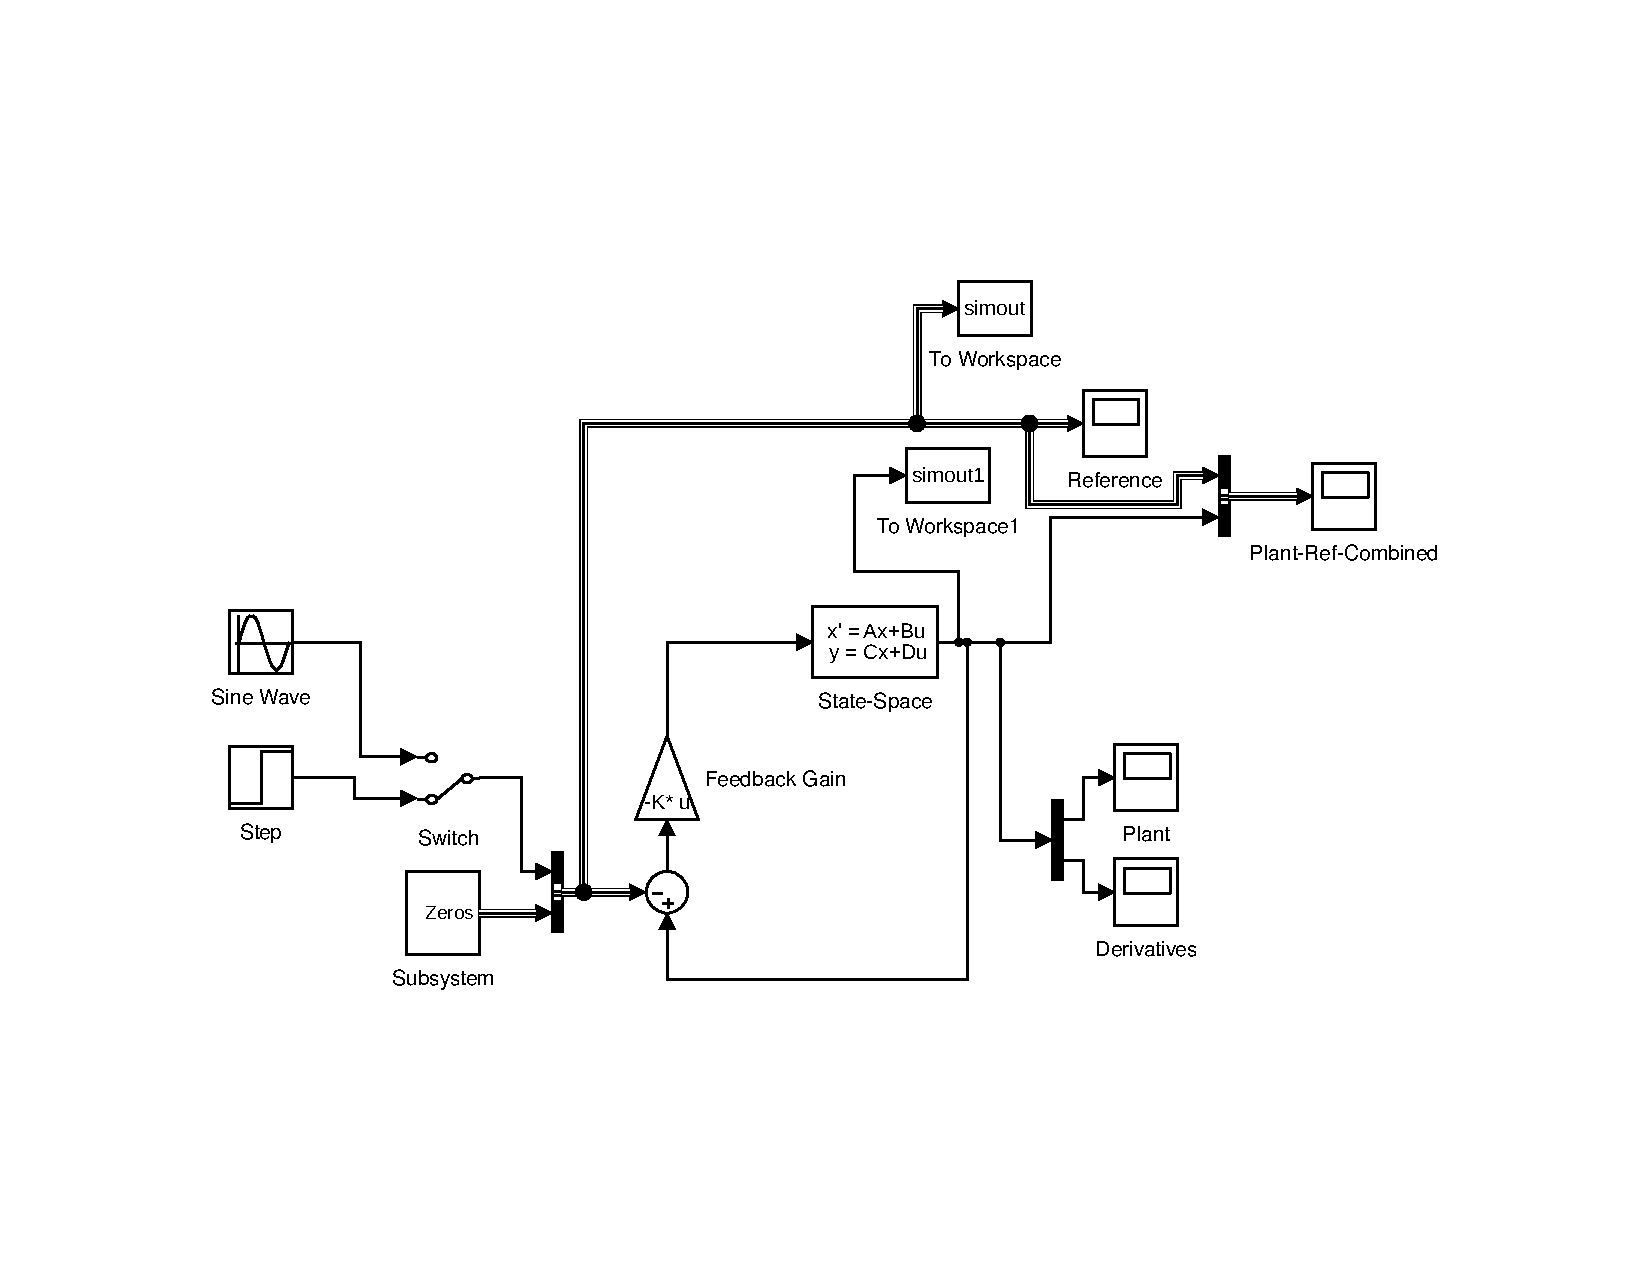
\includegraphics[scale=0.5]{images/simModelFullState.pdf}
\caption{The simulink Layout of our Simulation knowledge of all the states is assumed}
\label{fig:allStates}
\end{figure}
Figure~\ref{fig:allStates} shows our initial simulink diagram. The most important block in the control gain, that does the actual LQR-Control. The state space block in the center contains the continuous time system we showed in the previous section. In the left we have a selector that we use to choose between either a step or a sinusodial input. Below it we use a block of constant zeros to full up remaining entries of the input vector. 
As stated earlier we are using LQR-Control in this project. To compute the gain matrix for an LQR-Controller determines an state-feedback gain which minimizes the following cost function:
\begin{equation}
J = \int(\mathbf{x}^T Q \mathbf{x} + \mathbf{u}^T R \mathbf{u})dt.
\end{equation}
Initial but not optimal Q and R where given. \marginpar{Q = diag([350 1500 3 0.5]) for R = 10.} The $Q$ matrix gives weight to the different elements of the state vector. In our case hub position, arm position, angular hub and angular arm velocity. The R matrix, in our case a scalar makes the input more expensive. Our goals for tuning the controller are to achieve a satisfactory tracking for the hub angle $\theta$ without overshoot, while keeping the movement of the arm $\alpha$ as low as possible. At the same time we want to avoid actuator saturation. These are obviously conflicting objectives. So a good compromise is required. Figure~\ref{fig:stepResponse} shows the performance of the initially provided weighting parameters. From the tracking point of view the performance is not bad, however the input signal almost exceeds 5 Volts, which will might lead to actuator saturation if applied to the real plant. We chose the following weighting matrix to fix this problem:
\begin{equation}
\begin{pmatrix}
500 &		&	&	\\
	&1000	&	&	\\
	&	&3	&	\\
	&	&	&10	\\
\end{pmatrix}
\end{equation}
With the input weight $R = 30$. We increased the weight on the inputs to prevent saturation. As a higher input weight will make high inputs more expensive we expected this to fix our saturation problem. Furthermore it turns out more effective to penalize the acceleration of $\dot{\alpha}$ in comparison to a high value for $\alpha$. This is the case because we know that the reference for $\alpha$ will always be zero. Putting a higher weight on arm-acceleration prevents the arm from moving too fast away from its zero reference. In figure~{\ref{fig:stepResponse} on the right side we show the simulated behavior with our adapted weights, where the tracking remains comparably fast. 


\begin{figure}
%% This file was created by matlab2tikz v0.4.7 running on MATLAB 8.4.
% Copyright (c) 2008--2014, Nico Schlömer <nico.schloemer@gmail.com>
% All rights reserved.
% Minimal pgfplots version: 1.3
% 
% The latest updates can be retrieved from
%   http://www.mathworks.com/matlabcentral/fileexchange/22022-matlab2tikz
% where you can also make suggestions and rate matlab2tikz.
% 
\documentclass[tikz]{standalone}
\usepackage{pgfplots}
\usepackage{grffile}
\pgfplotsset{compat=newest}
\usetikzlibrary{plotmarks}
\usepackage{amsmath}

\begin{document}
%
% defining custom colors
\definecolor{mycolor1}{rgb}{0.00000,0.44700,0.74100}%
\definecolor{mycolor2}{rgb}{0.85000,0.32500,0.09800}%
\definecolor{mycolor3}{rgb}{0.92900,0.69400,0.12500}%
%
\begin{tikzpicture}

\begin{axis}[%
width=1.8in,
height=1in,
scale only axis,
separate axis lines,
every outer x axis line/.append style={white!15!black},
every x tick label/.append style={font=\color{white!15!black}},
xmin=0,
xmax=5,
every outer y axis line/.append style={white!15!black},
every y tick label/.append style={font=\color{white!15!black}},
ymin=-0.2,
ymax=0.8,
name=plot1,
%title style={font=\bfseries},
ylabel={plant, reference [rad]}
]
\addplot [color=mycolor1,solid,forget plot]
  table[row sep=crcr]{0	0\\
0.005	0\\
0.01	0\\
0.015	0\\
0.02	0\\
0.025	0\\
0.03	0\\
0.035	0\\
0.04	0\\
0.045	0\\
0.05	0\\
0.055	0\\
0.06	0\\
0.065	0\\
0.07	0\\
0.075	0\\
0.08	0\\
0.085	0\\
0.09	0\\
0.095	0\\
0.1	0\\
0.105	0\\
0.11	0\\
0.115	0\\
0.12	0\\
0.125	0\\
0.13	0\\
0.135	0\\
0.14	0\\
0.145	0\\
0.15	0\\
0.155	0\\
0.16	0\\
0.165	0\\
0.17	0\\
0.175	0\\
0.18	0\\
0.185	0\\
0.19	0\\
0.195	0\\
0.2	0\\
0.205	0\\
0.21	0\\
0.215	0\\
0.22	0\\
0.225	0\\
0.23	0\\
0.235	0\\
0.24	0\\
0.245	0\\
0.25	0\\
0.255	0\\
0.26	0\\
0.265	0\\
0.27	0\\
0.275	0\\
0.28	0\\
0.285	0\\
0.29	0\\
0.295	0\\
0.3	0\\
0.305	0\\
0.31	0\\
0.315	0\\
0.32	0\\
0.325	0\\
0.33	0\\
0.335	0\\
0.34	0\\
0.345	0\\
0.35	0\\
0.355	0\\
0.36	0\\
0.365	0\\
0.37	0\\
0.375	0\\
0.38	0\\
0.385	0\\
0.39	0\\
0.395	0\\
0.4	0\\
0.405	0\\
0.41	0\\
0.415	0\\
0.42	0\\
0.425	0\\
0.43	0\\
0.435	0\\
0.44	0\\
0.445	0\\
0.45	0\\
0.455	0\\
0.46	0\\
0.465	0\\
0.47	0\\
0.475	0\\
0.48	0\\
0.485	0\\
0.49	0\\
0.495	0\\
0.5	0\\
0.505	0\\
0.51	0\\
0.515	0\\
0.52	0\\
0.525	0\\
0.53	0\\
0.535	0\\
0.54	0\\
0.545	0\\
0.55	0\\
0.555	0\\
0.56	0\\
0.565	0\\
0.57	0\\
0.575	0\\
0.58	0\\
0.585	0\\
0.59	0\\
0.595	0\\
0.6	0\\
0.605	0\\
0.61	0\\
0.615	0\\
0.62	0\\
0.625	0\\
0.63	0\\
0.635	0\\
0.64	0\\
0.645	0\\
0.65	0\\
0.655	0\\
0.66	0\\
0.665	0\\
0.67	0\\
0.675	0\\
0.68	0\\
0.685	0\\
0.69	0\\
0.695	0\\
0.7	0\\
0.705	0\\
0.71	0\\
0.715	0\\
0.72	0\\
0.725	0\\
0.73	0\\
0.735	0\\
0.74	0\\
0.745	0\\
0.75	0\\
0.755	0\\
0.76	0\\
0.765	0\\
0.77	0\\
0.775	0\\
0.78	0\\
0.785	0\\
0.79	0\\
0.795	0\\
0.8	0\\
0.805	0\\
0.81	0\\
0.815	0\\
0.82	0\\
0.825	0\\
0.83	0\\
0.835	0\\
0.84	0\\
0.845	0\\
0.85	0\\
0.855	0\\
0.86	0\\
0.865	0\\
0.87	0\\
0.875	0\\
0.88	0\\
0.885	0\\
0.89	0\\
0.895	0\\
0.9	0\\
0.905	0\\
0.91	0\\
0.915	0\\
0.92	0\\
0.925	0\\
0.93	0\\
0.935	0\\
0.94	0\\
0.945	0\\
0.95	0\\
0.955	0\\
0.96	0\\
0.965	0\\
0.97	0\\
0.975	0\\
0.98	0\\
0.985	0\\
0.99	0\\
0.995	0\\
1	0\\
1.005	0.00523203624393392\\
1.01	0.018186605839208\\
1.015	0.0352342868591856\\
1.02	0.0539958675836227\\
1.025	0.0729538401874592\\
1.03	0.0911814985665003\\
1.035	0.108154164435518\\
1.04	0.123617771729083\\
1.045	0.137497513309732\\
1.05	0.149834471777402\\
1.055	0.160741798933166\\
1.06	0.170374551688914\\
1.065	0.178909067882093\\
1.07	0.18652900528233\\
1.075	0.193416032833595\\
1.08	0.199743767790938\\
1.085	0.205673974718829\\
1.09	0.211354337351883\\
1.095	0.216917320495604\\
1.1	0.222479783283137\\
1.105	0.228143105925134\\
1.11	0.233993662662367\\
1.115	0.240103523077566\\
1.12	0.24653129861244\\
1.125	0.253323075513464\\
1.13	0.260513392599091\\
1.135	0.268126234367861\\
1.14	0.276176018563894\\
1.145	0.284668563439095\\
1.15	0.293602024337562\\
1.155	0.302967792391718\\
1.16	0.312751350421486\\
1.165	0.322933082818445\\
1.17	0.333489037452368\\
1.175	0.344391638580611\\
1.18	0.355610350457881\\
1.185	0.367112291895478\\
1.19	0.378862802447752\\
1.195	0.39082596123959\\
1.2	0.402965059713482\\
1.205	0.415243029783715\\
1.21	0.427622829049477\\
1.215	0.440067784846418\\
1.22	0.452541899013558\\
1.225	0.465010115324052\\
1.23	0.477438551577801\\
1.235	0.489794698384265\\
1.24	0.502047586677305\\
1.245	0.514167926002721\\
1.25	0.526128215604857\\
1.255	0.537902830313022\\
1.26	0.54946808319269\\
1.265	0.560802266881934\\
1.27	0.571885675481361\\
1.275	0.582700608807132\\
1.28	0.593231360752331\\
1.285	0.603464193433073\\
1.29	0.613387298723041\\
1.295	0.6229907487045\\
1.3	0.632266436485938\\
1.305	0.641208008757046\\
1.31	0.649810791371382\\
1.315	0.658071709166338\\
1.32	0.665989201149497\\
1.325	0.673563132100536\\
1.33	0.680794701559025\\
1.335	0.687686351091074\\
1.34	0.694241670652191\\
1.345	0.700465304790197\\
1.35	0.706362859360872\\
1.355	0.711940809360391\\
1.36	0.717206408412709\\
1.365	0.722167600387061\\
1.37	0.726832933560775\\
1.375	0.731211477685625\\
1.38	0.735312744262281\\
1.385	0.739146610276779\\
1.39	0.74272324560561\\
1.395	0.746053044251857\\
1.4	0.749146559533802\\
1.405	0.752014443309568\\
1.41	0.754667389286558\\
1.415	0.757116080432633\\
1.42	0.759371140477116\\
1.425	0.76144308946361\\
1.43	0.763342303293271\\
1.435	0.765078977176455\\
1.44	0.766663092892383\\
1.445	0.768104389740616\\
1.45	0.769412339054492\\
1.455	0.770596122135182\\
1.46	0.771664611455526\\
1.465	0.772626354975165\\
1.47	0.773489563402598\\
1.475	0.774262100235515\\
1.48	0.774951474407985\\
1.485	0.77556483537163\\
1.49	0.776108970437781\\
1.495	0.776590304208553\\
1.5	0.777014899926774\\
1.505	0.777388462577599\\
1.51	0.777716343578334\\
1.515	0.77800354689743\\
1.52	0.77825473644863\\
1.525	0.778474244611791\\
1.53	0.77866608173794\\
1.535	0.778833946502436\\
1.54	0.778981236976806\\
1.545	0.779111062296642\\
1.55	0.779226254810009\\
1.555	0.779329382597903\\
1.56	0.779422762265478\\
1.565	0.779508471909898\\
1.57	0.779588364177768\\
1.575	0.779664079332135\\
1.58	0.77973705825588\\
1.585	0.779808555325088\\
1.59	0.779879651092488\\
1.595	0.779951264727374\\
1.6	0.780024166164523\\
1.605	0.780098987920441\\
1.61	0.780176236540865\\
1.615	0.780256303648721\\
1.62	0.780339476566789\\
1.625	0.780425948494016\\
1.63	0.780515828218898\\
1.635	0.780609149357447\\
1.64	0.780705879107156\\
1.645	0.780805926511913\\
1.65	0.780909150236081\\
1.655	0.781015365848986\\
1.66	0.781124352623757\\
1.665	0.781235859856914\\
1.67	0.781349612717323\\
1.675	0.78146531763506\\
1.68	0.781582667242469\\
1.685	0.781701344881166\\
1.69	0.781821028690034\\
1.695	0.781941395290304\\
1.7	0.782062123084725\\
1.705	0.78218289518849\\
1.71	0.782303402010148\\
1.715	0.782423343501092\\
1.72	0.782542431092445\\
1.725	0.782660389338271\\
1.73	0.782776957284001\\
1.735	0.782891889578862\\
1.74	0.783004957350819\\
1.745	0.783115948862261\\
1.75	0.78322466996424\\
1.755	0.783330944366603\\
1.76	0.783434613740823\\
1.765	0.783535537671783\\
1.77	0.783633593474079\\
1.775	0.783728675887817\\
1.78	0.783820696668139\\
1.785	0.783909584082021\\
1.79	0.783995282325145\\
1.795	0.784077750870941\\
1.8	0.784156963763106\\
1.805	0.784232908862202\\
1.81	0.784305587056185\\
1.815	0.784375011443996\\
1.82	0.78444120650061\\
1.825	0.784504207231271\\
1.83	0.784564058321931\\
1.835	0.784620813292271\\
1.84	0.784674533657029\\
1.845	0.784725288100765\\
1.85	0.784773151670588\\
1.855	0.784818204990824\\
1.86	0.784860533503076\\
1.865	0.784900226734607\\
1.87	0.784937377597525\\
1.875	0.784972081720795\\
1.88	0.785004436816686\\
1.885	0.785034542082893\\
1.89	0.785062497641197\\
1.895	0.785088404013206\\
1.9	0.785112361633437\\
1.905	0.785134470399696\\
1.91	0.785154829260488\\
1.915	0.785173535838968\\
1.92	0.785190686092727\\
1.925	0.785206374008561\\
1.93	0.78522069133119\\
1.935	0.785233727324798\\
1.94	0.785245568566103\\
1.945	0.78525629876764\\
1.95	0.785265998629796\\
1.955	0.785274745720137\\
1.96	0.785282614378482\\
1.965	0.785289675646162\\
1.97	0.7852959972179\\
1.975	0.785301643414729\\
1.98	0.785306675176356\\
1.985	0.785311150071437\\
1.99	0.785315122324208\\
1.995	0.785318642855978\\
2	0.785321759340015\\
2.005	0.78532451626841\\
2.01	0.785326955029534\\
2.015	0.785329113994788\\
2.02	0.785331028613374\\
2.025	0.78533273151389\\
2.03	0.78533425261161\\
2.035	0.785335619220382\\
2.04	0.785336856168125\\
2.045	0.785337985914983\\
2.05	0.785339028673272\\
2.055	0.785340002528383\\
2.06	0.785340923559915\\
2.065	0.78534180596234\\
2.07	0.785342662164581\\
2.075	0.785343502947937\\
2.08	0.785344337561857\\
2.085	0.785345173837105\\
2.09	0.785346018295934\\
2.095	0.785346876258912\\
2.1	0.78534775194812\\
2.105	0.785348648586466\\
2.11	0.785349568492922\\
2.115	0.785350513173509\\
2.12	0.785351483407917\\
2.125	0.785352479331678\\
2.13	0.785353500513823\\
2.135	0.785354546030014\\
2.14	0.785355614531151\\
2.145	0.785356704307484\\
2.15	0.78535781334829\\
2.155	0.78535893939718\\
2.16	0.785360080003136\\
2.165	0.785361232567392\\
2.17	0.785362394386272\\
2.175	0.785363562690125\\
2.18	0.785364734678508\\
2.185	0.785365907551767\\
2.19	0.785367078539178\\
2.195	0.785368244923816\\
2.2	0.785369404064316\\
2.205	0.785370553413718\\
2.21	0.785371690535539\\
2.215	0.785372813117282\\
2.22	0.785373918981522\\
2.225	0.785375006094763\\
2.23	0.785376072574228\\
2.235	0.785377116692744\\
2.24	0.785378136881882\\
2.245	0.785379131733512\\
2.25	0.785380099999932\\
2.255	0.785381040592688\\
2.26	0.785381952580263\\
2.265	0.785382835184734\\
2.27	0.785383687777546\\
2.275	0.785384509874504\\
2.28	0.78538530113012\\
2.285	0.785386061331391\\
2.29	0.785386790391139\\
2.295	0.785387488340977\\
2.3	0.785388155324007\\
2.305	0.785388791587321\\
2.31	0.785389397474376\\
2.315	0.785389973417313\\
2.32	0.785390519929282\\
2.325	0.785391037596823\\
2.33	0.785391527072348\\
2.335	0.785391989066783\\
2.34	0.785392424342393\\
2.345	0.78539283370582\\
2.35	0.785393218001386\\
2.355	0.785393578104653\\
2.36	0.785393914916288\\
2.365	0.785394229356231\\
2.37	0.785394522358185\\
2.375	0.785394794864438\\
2.38	0.785395047821019\\
2.385	0.785395282173194\\
2.39	0.785395498861305\\
2.395	0.785395698816941\\
2.4	0.78539588295945\\
2.405	0.785396052192773\\
2.41	0.785396207402604\\
2.415	0.785396349453858\\
2.42	0.785396479188447\\
2.425	0.785396597423339\\
2.43	0.785396704948898\\
2.435	0.785396802527497\\
2.44	0.785396890892372\\
2.445	0.785396970746724\\
2.45	0.785397042763039\\
2.455	0.785397107582619\\
2.46	0.785397165815315\\
2.465	0.78539721803943\\
2.47	0.785397264801799\\
2.475	0.785397306618015\\
2.48	0.7853973439728\\
2.485	0.785397377320492\\
2.49	0.785397407085656\\
2.495	0.785397433663786\\
2.5	0.785397457422097\\
2.505	0.785397478700395\\
2.51	0.785397497812007\\
2.515	0.785397515044773\\
2.52	0.785397530662071\\
2.525	0.785397544903887\\
2.53	0.785397557987906\\
2.535	0.785397570110621\\
2.54	0.785397581448456\\
2.545	0.785397592158884\\
2.55	0.785397602381552\\
2.555	0.785397612239389\\
2.56	0.785397621839705\\
2.565	0.785397631275267\\
2.57	0.785397640625354\\
2.575	0.785397649956785\\
2.58	0.785397659324914\\
2.585	0.7853976687746\\
2.59	0.785397678341126\\
2.595	0.785397688051099\\
2.6	0.785397697923299\\
2.605	0.785397707969492\\
2.61	0.785397718195201\\
2.615	0.785397728600433\\
2.62	0.785397739180374\\
2.625	0.78539774992603\\
2.63	0.785397760824829\\
2.635	0.785397771861194\\
2.64	0.785397783017055\\
2.645	0.78539779427234\\
2.65	0.785397805605418\\
2.655	0.785397816993503\\
2.66	0.785397828413028\\
2.665	0.785397839839982\\
2.67	0.785397851250207\\
2.675	0.785397862619673\\
2.68	0.785397873924715\\
2.685	0.785397885142243\\
2.69	0.785397896249929\\
2.695	0.785397907226357\\
2.7	0.785397918051163\\
2.705	0.785397928705142\\
2.71	0.785397939170336\\
2.715	0.785397949430106\\
2.72	0.785397959469181\\
2.725	0.785397969273698\\
2.73	0.785397978831216\\
2.735	0.785397988130727\\
2.74	0.78539799716265\\
2.745	0.785398005918811\\
2.75	0.78539801439242\\
2.755	0.785398022578034\\
2.76	0.785398030471516\\
2.765	0.785398038069983\\
2.77	0.785398045371758\\
2.775	0.785398052376303\\
2.78	0.785398059084163\\
2.785	0.785398065496899\\
2.79	0.78539807161702\\
2.795	0.785398077447913\\
2.8	0.78539808299378\\
2.805	0.78539808825956\\
2.81	0.785398093250866\\
2.815	0.785398097973915\\
2.82	0.78539810243546\\
2.825	0.785398106642725\\
2.83	0.785398110603344\\
2.835	0.785398114325294\\
2.84	0.785398117816842\\
2.845	0.785398121086484\\
2.85	0.785398124142895\\
2.855	0.785398126994876\\
2.86	0.785398129651306\\
2.865	0.785398132121101\\
2.87	0.785398134413167\\
2.875	0.785398136536364\\
2.88	0.785398138499473\\
2.885	0.785398140311161\\
2.89	0.785398141979949\\
2.895	0.785398143514191\\
2.9	0.785398144922048\\
2.905	0.785398146211468\\
2.91	0.785398147390164\\
2.915	0.785398148465604\\
2.92	0.785398149444996\\
2.925	0.785398150335274\\
2.93	0.785398151143095\\
2.935	0.785398151874828\\
2.94	0.785398152536551\\
2.945	0.785398153134051\\
2.95	0.785398153672817\\
2.955	0.785398154158047\\
2.96	0.785398154594644\\
2.965	0.785398154987226\\
2.97	0.785398155340123\\
2.975	0.785398155657388\\
2.98	0.785398155942801\\
2.985	0.785398156199878\\
2.99	0.785398156431877\\
2.995	0.785398156641805\\
3	0.785398156832434\\
3.005	0.785398157006303\\
3.01	0.78539815716573\\
3.015	0.785398157312826\\
3.02	0.7853981574495\\
3.025	0.785398157577471\\
3.03	0.78539815769828\\
3.035	0.785398157813301\\
3.04	0.785398157923745\\
3.045	0.785398158030681\\
3.05	0.785398158135034\\
3.055	0.785398158237605\\
3.06	0.785398158339074\\
3.065	0.785398158440012\\
3.07	0.785398158540892\\
3.075	0.785398158642092\\
3.08	0.785398158743908\\
3.085	0.785398158846562\\
3.09	0.785398158950206\\
3.095	0.785398159054932\\
3.1	0.785398159160781\\
3.105	0.785398159267743\\
3.11	0.78539815937577\\
3.115	0.785398159484776\\
3.12	0.785398159594648\\
3.125	0.785398159705247\\
3.13	0.78539815981641\\
3.135	0.785398159927963\\
3.14	0.785398160039717\\
3.145	0.785398160151473\\
3.15	0.785398160263029\\
3.155	0.785398160374178\\
3.16	0.785398160484713\\
3.165	0.785398160594431\\
3.17	0.785398160703132\\
3.175	0.785398160810621\\
3.18	0.785398160916711\\
3.185	0.785398161021225\\
3.19	0.785398161123993\\
3.195	0.78539816122486\\
3.2	0.785398161323678\\
3.205	0.785398161420315\\
3.21	0.785398161514647\\
3.215	0.785398161606566\\
3.22	0.785398161695977\\
3.225	0.785398161782794\\
3.23	0.785398161866948\\
3.235	0.785398161948379\\
3.24	0.785398162027042\\
3.245	0.785398162102901\\
3.25	0.785398162175934\\
3.255	0.785398162246127\\
3.26	0.785398162313479\\
3.265	0.785398162377998\\
3.27	0.7853981624397\\
3.275	0.785398162498611\\
3.28	0.785398162554765\\
3.285	0.785398162608202\\
3.29	0.785398162658971\\
3.295	0.785398162707125\\
3.3	0.785398162752723\\
3.305	0.785398162795831\\
3.31	0.785398162836516\\
3.315	0.785398162874852\\
3.32	0.785398162910913\\
3.325	0.785398162944777\\
3.33	0.785398162976526\\
3.335	0.785398163006241\\
3.34	0.785398163034005\\
3.345	0.785398163059902\\
3.35	0.785398163084015\\
3.355	0.78539816310643\\
3.36	0.785398163127229\\
3.365	0.785398163146496\\
3.37	0.785398163164312\\
3.375	0.785398163180758\\
3.38	0.785398163195912\\
3.385	0.785398163209851\\
3.39	0.785398163222652\\
3.395	0.785398163234386\\
3.4	0.785398163245124\\
3.405	0.785398163254934\\
3.41	0.785398163263882\\
3.415	0.785398163272031\\
3.42	0.785398163279442\\
3.425	0.785398163286172\\
3.43	0.785398163292275\\
3.435	0.785398163297805\\
3.44	0.78539816330281\\
3.445	0.785398163307338\\
3.45	0.785398163311431\\
3.455	0.785398163315132\\
3.46	0.785398163318479\\
3.465	0.785398163321509\\
3.47	0.785398163324254\\
3.475	0.785398163326747\\
3.48	0.785398163329016\\
3.485	0.785398163331087\\
3.49	0.785398163332986\\
3.495	0.785398163334735\\
3.5	0.785398163336353\\
3.505	0.78539816333786\\
3.51	0.785398163339273\\
3.515	0.785398163340606\\
3.52	0.785398163341873\\
3.525	0.785398163343086\\
3.53	0.785398163344255\\
3.535	0.78539816334539\\
3.54	0.785398163346499\\
3.545	0.785398163347589\\
3.55	0.785398163348665\\
3.555	0.785398163349732\\
3.56	0.785398163350795\\
3.565	0.785398163351857\\
3.57	0.785398163352919\\
3.575	0.785398163353985\\
3.58	0.785398163355055\\
3.585	0.78539816335613\\
3.59	0.785398163357211\\
3.595	0.785398163358296\\
3.6	0.785398163359386\\
3.605	0.785398163360481\\
3.61	0.785398163361578\\
3.615	0.785398163362676\\
3.62	0.785398163363775\\
3.625	0.785398163364873\\
3.63	0.785398163365968\\
3.635	0.785398163367058\\
3.64	0.785398163368142\\
3.645	0.785398163369219\\
3.65	0.785398163370285\\
3.655	0.785398163371339\\
3.66	0.785398163372381\\
3.665	0.785398163373408\\
3.67	0.785398163374418\\
3.675	0.78539816337541\\
3.68	0.785398163376384\\
3.685	0.785398163377337\\
3.69	0.785398163378268\\
3.695	0.785398163379176\\
3.7	0.785398163380061\\
3.705	0.785398163380922\\
3.71	0.785398163381757\\
3.715	0.785398163382567\\
3.72	0.78539816338335\\
3.725	0.785398163384107\\
3.73	0.785398163384836\\
3.735	0.785398163385539\\
3.74	0.785398163386214\\
3.745	0.785398163386863\\
3.75	0.785398163387484\\
3.755	0.785398163388078\\
3.76	0.785398163388645\\
3.765	0.785398163389186\\
3.77	0.785398163389702\\
3.775	0.785398163390191\\
3.78	0.785398163390656\\
3.785	0.785398163391097\\
3.79	0.785398163391513\\
3.795	0.785398163391907\\
3.8	0.785398163392278\\
3.805	0.785398163392628\\
3.81	0.785398163392956\\
3.815	0.785398163393265\\
3.82	0.785398163393554\\
3.825	0.785398163393824\\
3.83	0.785398163394077\\
3.835	0.785398163394312\\
3.84	0.785398163394531\\
3.845	0.785398163394735\\
3.85	0.785398163394924\\
3.855	0.785398163395099\\
3.86	0.785398163395261\\
3.865	0.785398163395411\\
3.87	0.785398163395548\\
3.875	0.785398163395675\\
3.88	0.785398163395792\\
3.885	0.785398163395899\\
3.89	0.785398163395997\\
3.895	0.785398163396087\\
3.9	0.785398163396169\\
3.905	0.785398163396244\\
3.91	0.785398163396312\\
3.915	0.785398163396374\\
3.92	0.785398163396431\\
3.925	0.785398163396482\\
3.93	0.785398163396529\\
3.935	0.785398163396571\\
3.94	0.78539816339661\\
3.945	0.785398163396645\\
3.95	0.785398163396676\\
3.955	0.785398163396705\\
3.96	0.785398163396732\\
3.965	0.785398163396756\\
3.97	0.785398163396778\\
3.975	0.785398163396799\\
3.98	0.785398163396818\\
3.985	0.785398163396835\\
3.99	0.785398163396852\\
3.995	0.785398163396867\\
4	0.785398163396881\\
4.005	0.785398163396895\\
4.01	0.785398163396908\\
4.015	0.785398163396921\\
4.02	0.785398163396933\\
4.025	0.785398163396945\\
4.03	0.785398163396956\\
4.035	0.785398163396968\\
4.04	0.785398163396979\\
4.045	0.78539816339699\\
4.05	0.785398163397001\\
4.055	0.785398163397012\\
4.06	0.785398163397023\\
4.065	0.785398163397034\\
4.07	0.785398163397045\\
4.075	0.785398163397056\\
4.08	0.785398163397066\\
4.085	0.785398163397077\\
4.09	0.785398163397088\\
4.095	0.785398163397099\\
4.1	0.78539816339711\\
4.105	0.785398163397121\\
4.11	0.785398163397132\\
4.115	0.785398163397142\\
4.12	0.785398163397153\\
4.125	0.785398163397164\\
4.13	0.785398163397174\\
4.135	0.785398163397184\\
4.14	0.785398163397195\\
4.145	0.785398163397205\\
4.15	0.785398163397215\\
4.155	0.785398163397225\\
4.16	0.785398163397234\\
4.165	0.785398163397244\\
4.17	0.785398163397253\\
4.175	0.785398163397262\\
4.18	0.785398163397271\\
4.185	0.785398163397279\\
4.19	0.785398163397288\\
4.195	0.785398163397296\\
4.2	0.785398163397303\\
4.205	0.785398163397311\\
4.21	0.785398163397318\\
4.215	0.785398163397325\\
4.22	0.785398163397332\\
4.225	0.785398163397339\\
4.23	0.785398163397345\\
4.235	0.785398163397351\\
4.24	0.785398163397357\\
4.245	0.785398163397362\\
4.25	0.785398163397367\\
4.255	0.785398163397372\\
4.26	0.785398163397377\\
4.265	0.785398163397381\\
4.27	0.785398163397386\\
4.275	0.78539816339739\\
4.28	0.785398163397393\\
4.285	0.785398163397397\\
4.29	0.7853981633974\\
4.295	0.785398163397404\\
4.3	0.785398163397407\\
4.305	0.785398163397409\\
4.31	0.785398163397412\\
4.315	0.785398163397415\\
4.32	0.785398163397417\\
4.325	0.785398163397419\\
4.33	0.785398163397421\\
4.335	0.785398163397423\\
4.34	0.785398163397425\\
4.345	0.785398163397426\\
4.35	0.785398163397428\\
4.355	0.785398163397429\\
4.36	0.78539816339743\\
4.365	0.785398163397431\\
4.37	0.785398163397432\\
4.375	0.785398163397433\\
4.38	0.785398163397434\\
4.385	0.785398163397435\\
4.39	0.785398163397436\\
4.395	0.785398163397437\\
4.4	0.785398163397437\\
4.405	0.785398163397438\\
4.41	0.785398163397438\\
4.415	0.785398163397439\\
4.42	0.785398163397439\\
4.425	0.78539816339744\\
4.43	0.78539816339744\\
4.435	0.78539816339744\\
4.44	0.785398163397441\\
4.445	0.785398163397441\\
4.45	0.785398163397441\\
4.455	0.785398163397441\\
4.46	0.785398163397442\\
4.465	0.785398163397442\\
4.47	0.785398163397442\\
4.475	0.785398163397442\\
4.48	0.785398163397442\\
4.485	0.785398163397443\\
4.49	0.785398163397443\\
4.495	0.785398163397443\\
4.5	0.785398163397443\\
4.505	0.785398163397443\\
4.51	0.785398163397443\\
4.515	0.785398163397443\\
4.52	0.785398163397443\\
4.525	0.785398163397443\\
4.53	0.785398163397444\\
4.535	0.785398163397444\\
4.54	0.785398163397444\\
4.545	0.785398163397444\\
4.55	0.785398163397444\\
4.555	0.785398163397444\\
4.56	0.785398163397444\\
4.565	0.785398163397444\\
4.57	0.785398163397444\\
4.575	0.785398163397445\\
4.58	0.785398163397445\\
4.585	0.785398163397445\\
4.59	0.785398163397445\\
4.595	0.785398163397445\\
4.6	0.785398163397445\\
4.605	0.785398163397445\\
4.61	0.785398163397445\\
4.615	0.785398163397445\\
4.62	0.785398163397446\\
4.625	0.785398163397446\\
4.63	0.785398163397446\\
4.635	0.785398163397446\\
4.64	0.785398163397446\\
4.645	0.785398163397446\\
4.65	0.785398163397446\\
4.655	0.785398163397446\\
4.66	0.785398163397446\\
4.665	0.785398163397447\\
4.67	0.785398163397447\\
4.675	0.785398163397447\\
4.68	0.785398163397447\\
4.685	0.785398163397447\\
4.69	0.785398163397447\\
4.695	0.785398163397447\\
4.7	0.785398163397447\\
4.705	0.785398163397447\\
4.71	0.785398163397448\\
4.715	0.785398163397448\\
4.72	0.785398163397448\\
4.725	0.785398163397448\\
4.73	0.785398163397448\\
4.735	0.785398163397448\\
4.74	0.785398163397448\\
4.745	0.785398163397448\\
4.75	0.785398163397448\\
4.755	0.785398163397448\\
4.76	0.785398163397448\\
4.765	0.785398163397448\\
4.77	0.785398163397448\\
4.775	0.785398163397448\\
4.78	0.785398163397448\\
4.785	0.785398163397448\\
4.79	0.785398163397448\\
4.795	0.785398163397448\\
4.8	0.785398163397448\\
4.805	0.785398163397448\\
4.81	0.785398163397448\\
4.815	0.785398163397448\\
4.82	0.785398163397448\\
4.825	0.785398163397448\\
4.83	0.785398163397448\\
4.835	0.785398163397448\\
4.84	0.785398163397448\\
4.845	0.785398163397448\\
4.85	0.785398163397448\\
4.855	0.785398163397448\\
4.86	0.785398163397448\\
4.865	0.785398163397448\\
4.87	0.785398163397448\\
4.875	0.785398163397448\\
4.88	0.785398163397448\\
4.885	0.785398163397448\\
4.89	0.785398163397448\\
4.895	0.785398163397448\\
4.9	0.785398163397448\\
4.905	0.785398163397448\\
4.91	0.785398163397448\\
4.915	0.785398163397448\\
4.92	0.785398163397448\\
4.925	0.785398163397448\\
4.93	0.785398163397448\\
4.935	0.785398163397448\\
4.94	0.785398163397448\\
4.945	0.785398163397448\\
4.95	0.785398163397448\\
4.955	0.785398163397448\\
4.96	0.785398163397448\\
4.965	0.785398163397448\\
4.97	0.785398163397448\\
4.975	0.785398163397448\\
4.98	0.785398163397448\\
4.985	0.785398163397448\\
4.99	0.785398163397448\\
4.995	0.785398163397448\\
5	0.785398163397448\\
};
\addplot [color=mycolor2,solid,forget plot]
  table[row sep=crcr]{0	0\\
0.005	0\\
0.01	0\\
0.015	0\\
0.02	0\\
0.025	0\\
0.03	0\\
0.035	0\\
0.04	0\\
0.045	0\\
0.05	0\\
0.055	0\\
0.06	0\\
0.065	0\\
0.07	0\\
0.075	0\\
0.08	0\\
0.085	0\\
0.09	0\\
0.095	0\\
0.1	0\\
0.105	0\\
0.11	0\\
0.115	0\\
0.12	0\\
0.125	0\\
0.13	0\\
0.135	0\\
0.14	0\\
0.145	0\\
0.15	0\\
0.155	0\\
0.16	0\\
0.165	0\\
0.17	0\\
0.175	0\\
0.18	0\\
0.185	0\\
0.19	0\\
0.195	0\\
0.2	0\\
0.205	0\\
0.21	0\\
0.215	0\\
0.22	0\\
0.225	0\\
0.23	0\\
0.235	0\\
0.24	0\\
0.245	0\\
0.25	0\\
0.255	0\\
0.26	0\\
0.265	0\\
0.27	0\\
0.275	0\\
0.28	0\\
0.285	0\\
0.29	0\\
0.295	0\\
0.3	0\\
0.305	0\\
0.31	0\\
0.315	0\\
0.32	0\\
0.325	0\\
0.33	0\\
0.335	0\\
0.34	0\\
0.345	0\\
0.35	0\\
0.355	0\\
0.36	0\\
0.365	0\\
0.37	0\\
0.375	0\\
0.38	0\\
0.385	0\\
0.39	0\\
0.395	0\\
0.4	0\\
0.405	0\\
0.41	0\\
0.415	0\\
0.42	0\\
0.425	0\\
0.43	0\\
0.435	0\\
0.44	0\\
0.445	0\\
0.45	0\\
0.455	0\\
0.46	0\\
0.465	0\\
0.47	0\\
0.475	0\\
0.48	0\\
0.485	0\\
0.49	0\\
0.495	0\\
0.5	0\\
0.505	0\\
0.51	0\\
0.515	0\\
0.52	0\\
0.525	0\\
0.53	0\\
0.535	0\\
0.54	0\\
0.545	0\\
0.55	0\\
0.555	0\\
0.56	0\\
0.565	0\\
0.57	0\\
0.575	0\\
0.58	0\\
0.585	0\\
0.59	0\\
0.595	0\\
0.6	0\\
0.605	0\\
0.61	0\\
0.615	0\\
0.62	0\\
0.625	0\\
0.63	0\\
0.635	0\\
0.64	0\\
0.645	0\\
0.65	0\\
0.655	0\\
0.66	0\\
0.665	0\\
0.67	0\\
0.675	0\\
0.68	0\\
0.685	0\\
0.69	0\\
0.695	0\\
0.7	0\\
0.705	0\\
0.71	0\\
0.715	0\\
0.72	0\\
0.725	0\\
0.73	0\\
0.735	0\\
0.74	0\\
0.745	0\\
0.75	0\\
0.755	0\\
0.76	0\\
0.765	0\\
0.77	0\\
0.775	0\\
0.78	0\\
0.785	0\\
0.79	0\\
0.795	0\\
0.8	0\\
0.805	0\\
0.81	0\\
0.815	0\\
0.82	0\\
0.825	0\\
0.83	0\\
0.835	0\\
0.84	0\\
0.845	0\\
0.85	0\\
0.855	0\\
0.86	0\\
0.865	0\\
0.87	0\\
0.875	0\\
0.88	0\\
0.885	0\\
0.89	0\\
0.895	0\\
0.9	0\\
0.905	0\\
0.91	0\\
0.915	0\\
0.92	0\\
0.925	0\\
0.93	0\\
0.935	0\\
0.94	0\\
0.945	0\\
0.95	0\\
0.955	0\\
0.96	0\\
0.965	0\\
0.97	0\\
0.975	0\\
0.98	0\\
0.985	0\\
0.99	0\\
0.995	0\\
1	0\\
1.005	-0.00522895785388764\\
1.01	-0.018140478443417\\
1.015	-0.0350192359012344\\
1.02	-0.0533723828618899\\
1.025	-0.0715582452015607\\
1.03	-0.0885267561879355\\
1.035	-0.103637942408965\\
1.04	-0.116534941998379\\
1.045	-0.127055133947732\\
1.05	-0.13516791251939\\
1.055	-0.140931099966631\\
1.06	-0.144460405602637\\
1.065	-0.145908025051329\\
1.07	-0.145447650376318\\
1.075	-0.143263983380385\\
1.08	-0.139545417965598\\
1.085	-0.134478957925612\\
1.09	-0.128246716180759\\
1.095	-0.121023536753933\\
1.1	-0.112975417194006\\
1.105	-0.104258504464883\\
1.11	-0.0950185039444863\\
1.115	-0.085390387782719\\
1.12	-0.075498321498049\\
1.125	-0.065455750569575\\
1.13	-0.05536560485087\\
1.135	-0.0453205899492992\\
1.14	-0.0354035427141649\\
1.145	-0.0256878336598002\\
1.15	-0.0162378032135887\\
1.155	-0.00710922161080584\\
1.16	0.00165023560250704\\
1.165	0.010000502913985\\
1.17	0.0179086362997285\\
1.175	0.0253483251363851\\
1.18	0.0322994081977014\\
1.185	0.0387473967836846\\
1.19	0.0446830075534548\\
1.195	0.050101707230963\\
1.2	0.0550032710072106\\
1.205	0.0593913561604853\\
1.21	0.0632730921482778\\
1.215	0.0666586881846732\\
1.22	0.0695610591005942\\
1.225	0.0719954700881671\\
1.23	0.0739792007523578\\
1.235	0.0755312287312077\\
1.24	0.0766719329991639\\
1.245	0.0774228168351487\\
1.25	0.077806250317273\\
1.255	0.0778452320987489\\
1.26	0.0775631701239369\\
1.265	0.0769836808589477\\
1.27	0.0761304065372328\\
1.275	0.0750268498565632\\
1.28	0.0736962255091572\\
1.285	0.0721613278809166\\
1.29	0.0704444142182274\\
1.295	0.0685671025310246\\
1.3	0.0665502834782807\\
1.305	0.0644140454662276\\
1.31	0.0621776121799352\\
1.315	0.0598592917648495\\
1.32	0.0574764368760328\\
1.325	0.0550454148186787\\
1.33	0.0525815870135168\\
1.335	0.050099297034544\\
1.34	0.0476118664836674\\
1.345	0.0451315979869408\\
1.35	0.0426697846196868\\
1.355	0.040236725092595\\
1.36	0.0378417440574819\\
1.365	0.0354932169194905\\
1.37	0.0331985985717686\\
1.375	0.0309644554988204\\
1.38	0.0287965007254971\\
1.385	0.0266996311197464\\
1.39	0.024677966588538\\
1.395	0.0227348907376277\\
1.4	0.0208730925968228\\
1.405	0.0190946090430017\\
1.41	0.0174008675831654\\
1.415	0.0157927291891357\\
1.42	0.0142705309040324\\
1.425	0.0128341279682704\\
1.43	0.0114829352394329\\
1.435	0.0102159677059116\\
1.44	0.00903187991861981\\
1.445	0.00792900418831761\\
1.45	0.00690538741811721\\
1.455	0.00595882646152252\\
1.46	0.00508690191590359\\
1.465	0.00428701027958973\\
1.47	0.00355639441780429\\
1.475	0.00289217229845534\\
1.48	0.00229136397336926\\
1.485	0.00175091679392058\\
1.49	0.00126772886220925\\
1.495	0.000838670729990192\\
1.5	0.000460605367513933\\
1.505	0.000130406433325272\\
1.51	-0.000155025116062033\\
1.515	-0.000398746030802024\\
1.52	-0.000603757334882442\\
1.525	-0.000772992398947669\\
1.53	-0.000909306457643734\\
1.535	-0.00101546750686727\\
1.54	-0.00109414851354394\\
1.545	-0.00114792086848412\\
1.55	-0.0011792490114134\\
1.555	-0.00119048615640405\\
1.56	-0.00118387104559331\\
1.565	-0.00116152565921731\\
1.57	-0.00112545381057102\\
1.575	-0.0010775405554796\\
1.58	-0.00101955234719334\\
1.585	-0.000953137869255918\\
1.59	-0.000879829480804382\\
1.595	-0.000801045210903526\\
1.6	-0.000718091240860391\\
1.605	-0.000632164815974939\\
1.61	-0.000544357530828262\\
1.615	-0.000455658934961978\\
1.62	-0.000366960408633781\\
1.625	-0.000279059261220454\\
1.63	-0.000192663007756881\\
1.635	-0.00010839378202775\\
1.64	-2.67928475473982e-05\\
1.645	5.16748293437829e-05\\
1.65	0.00012661597718731\\
1.655	0.000197704418044603\\
1.66	0.000264676494463935\\
1.665	0.000327326549526926\\
1.67	0.000385502482165339\\
1.675	0.000439101397474669\\
1.68	0.000488065369389493\\
1.685	0.000532377330831662\\
1.69	0.000572057104300409\\
1.695	0.000607157583846495\\
1.7	0.000637761077462436\\
1.705	0.000663975817129083\\
1.71	0.000685932642085354\\
1.715	0.000703781859332588\\
1.72	0.00071769028394636\\
1.725	0.000727838460445189\\
1.73	0.000734418065254711\\
1.735	0.000737629489205171\\
1.74	0.000737679598005856\\
1.745	0.00073477966774909\\
1.75	0.000729143491704521\\
1.755	0.000720985653967529\\
1.76	0.000710519964919358\\
1.765	0.000697958052936402\\
1.77	0.000683508106347346\\
1.775	0.000667373759274831\\
1.78	0.000649753114708248\\
1.785	0.000630837897931253\\
1.79	0.000610812733267104\\
1.795	0.00058985453700194\\
1.8	0.000568132019296366\\
1.805	0.000545805287894259\\
1.81	0.000523025546480496\\
1.815	0.000499934880621796\\
1.82	0.000476666124342988\\
1.825	0.000453342800540877\\
1.83	0.000430079128615461\\
1.835	0.000406980092900161\\
1.84	0.000384141565695272\\
1.845	0.000361650478948966\\
1.85	0.000339585038884632\\
1.855	0.00031801497813937\\
1.86	0.000297001840253286\\
1.865	0.000276599291630453\\
1.87	0.000256853456377559\\
1.875	0.000237803269713471\\
1.88	0.000219480845929935\\
1.885	0.000201911857169036\\
1.89	0.000185115919564872\\
1.895	0.000169106983574085\\
1.9	0.000153893725590889\\
1.905	0.000139479938206159\\
1.91	0.000125864916725852\\
1.915	0.000113043839810828\\
1.92	0.000101008142337247\\
1.925	8.97458788036334e-05\\
1.93	7.92420758268851e-05\\
1.935	6.94790724747008e-05\\
1.94	6.04368473758028e-05\\
1.945	5.20933317317828e-05\\
1.95	4.44247075253877e-05\\
1.955	3.7405690379495e-05\\
1.96	3.10097966690984e-05\\
1.965	2.52095946253563e-05\\
1.97	1.99769392964517e-05\\
1.975	1.52831913448312e-05\\
1.98	1.10994197646934e-05\\
1.985	7.39658869765424e-06\\
1.99	4.14572860874558e-06\\
1.995	1.3180921596412e-06\\
2	-1.11470481829113e-06\\
2.005	-3.1805567914457e-06\\
2.01	-4.90675592337885e-06\\
2.015	-6.31989285642853e-06\\
2.02	-7.44577029192835e-06\\
2.025	-8.30932875829054e-06\\
2.03	-8.93458393548776e-06\\
2.035	-9.34457488959651e-06\\
2.04	-9.56132256163179e-06\\
2.045	-9.60579785045646e-06\\
2.05	-9.4978986296658e-06\\
2.055	-9.25643504258787e-06\\
2.06	-8.89912242750725e-06\\
2.065	-8.44258123651733e-06\\
2.07	-7.90234332565646e-06\\
2.075	-7.29286401081823e-06\\
2.08	-6.62753930300769e-06\\
2.085	-5.91872775751857e-06\\
2.09	-5.17777639421245e-06\\
2.095	-4.41505017000997e-06\\
2.1	-3.63996450968845e-06\\
2.105	-2.86102042684733e-06\\
2.11	-2.08584179324216e-06\\
2.115	-1.32121434136566e-06\\
2.12	-5.7312601198452e-07\\
2.125	1.53191714867308e-07\\
2.13	8.53221840343087e-07\\
2.135	1.52311952734204e-06\\
2.14	2.15966972405513e-06\\
2.145	2.76024498820731e-06\\
2.15	3.32276374522458e-06\\
2.155	3.84564918986133e-06\\
2.16	4.32778901798844e-06\\
2.165	4.76849615333599e-06\\
2.17	5.16747061305015e-06\\
2.175	5.52476263601e-06\\
2.18	5.84073717897642e-06\\
2.185	6.11603986784472e-06\\
2.19	6.35156447455492e-06\\
2.195	6.54842197458073e-06\\
2.2	6.70791122536605e-06\\
2.205	6.83149129259926e-06\\
2.21	6.92075543880555e-06\\
2.215	6.97740677735988e-06\\
2.22	7.00323558466241e-06\\
2.225	7.0000982538451e-06\\
2.23	6.96989786495623e-06\\
2.235	6.91456633907399e-06\\
2.24	6.83604813718026e-06\\
2.245	6.73628545884811e-06\\
2.25	6.61720489082249e-06\\
2.255	6.48070545135595e-06\\
2.26	6.32864797265922e-06\\
2.265	6.16284576099659e-06\\
2.27	5.98505647175259e-06\\
2.275	5.79697513517687e-06\\
2.28	5.60022826743396e-06\\
2.285	5.39636900100655e-06\\
2.29	5.18687316837395e-06\\
2.295	4.97313627317815e-06\\
2.3	4.75647128375359e-06\\
2.305	4.53810718490019e-06\\
2.31	4.31918822508032e-06\\
2.315	4.10077379778671e-06\\
2.32	3.88383889762658e-06\\
2.325	3.66927509366326e-06\\
2.33	3.45789196471968e-06\\
2.335	3.2504189436531e-06\\
2.34	3.04750752002368e-06\\
2.345	2.84973375308657e-06\\
2.35	2.65760104960526e-06\\
2.355	2.47154316358988e-06\\
2.36	2.29192737770028e-06\\
2.365	2.1190578286903e-06\\
2.37	1.95317894189257e-06\\
2.375	1.79447894234271e-06\\
2.38	1.64309341269872e-06\\
2.385	1.49910887061282e-06\\
2.39	1.3625663406543e-06\\
2.395	1.2334648982511e-06\\
2.4	1.11176516540796e-06\\
2.405	9.97392740155324e-07\\
2.41	8.90241543793707e-07\\
2.415	7.90177072009793e-07\\
2.42	6.97039537851557e-07\\
2.425	6.10646896356508e-07\\
2.43	5.30797742330643e-07\\
2.435	4.57274074375316e-07\\
2.44	3.89843919749738e-07\\
2.445	3.28263816042475e-07\\
2.45	2.72281146912053e-07\\
2.455	2.21636330335513e-07\\
2.46	1.76064858885086e-07\\
2.465	1.35299192535223e-07\\
2.47	9.90705053933882e-08\\
2.475	6.71102885443186e-08\\
2.48	3.91518119055222e-08\\
2.485	1.49314486181432e-08\\
2.49	-5.81013395706289e-09\\
2.495	-2.33269120983365e-08\\
2.5	-3.78665675034791e-08\\
2.505	-4.96696677260191e-08\\
2.51	-5.89689597377399e-08\\
2.515	-6.59887708824824e-08\\
2.52	-7.09445113317088e-08\\
2.525	-7.40422720548871e-08\\
2.53	-7.54785122646212e-08\\
2.535	-7.54398302863561e-08\\
2.54	-7.4102811829165e-08\\
2.545	-7.16339497006183e-08\\
2.55	-6.81896291012023e-08\\
2.555	-6.39161727593558e-08\\
2.56	-5.89499403161453e-08\\
2.565	-5.34174765344679e-08\\
2.57	-4.74357031013475e-08\\
2.575	-4.11121489921043e-08\\
2.58	-3.45452145788407e-08\\
2.585	-2.78244648970716e-08\\
2.59	-2.10309477160431e-08\\
2.595	-1.4237532300053e-08\\
2.6	-7.50926498928823e-09\\
2.605	-9.03737974868331e-10\\
2.61	5.52853210692388e-09\\
2.615	1.1743718897257e-08\\
2.62	1.77042972486609e-08\\
2.625	2.33786530225583e-08\\
2.63	2.87406941733195e-08\\
2.635	3.3769465317432e-08\\
2.64	3.84487677618899e-08\\
2.645	4.27667867596477e-08\\
2.65	4.67157275551998e-08\\
2.655	5.02914615874856e-08\\
2.66	5.3493184031976e-08\\
2.665	5.63230836911124e-08\\
2.67	5.87860260756139e-08\\
2.675	6.08892503611512e-08\\
2.68	6.26420807590315e-08\\
2.685	6.40556527050468e-08\\
2.69	6.51426541462239e-08\\
2.695	6.59170820849327e-08\\
2.7	6.63940144329667e-08\\
2.705	6.65893971338027e-08\\
2.71	6.6519846423106e-08\\
2.715	6.62024660135084e-08\\
2.72	6.5654678923354e-08\\
2.725	6.48940736047834e-08\\
2.73	6.39382639692457e-08\\
2.735	6.28047628644637e-08\\
2.74	6.15108685152921e-08\\
2.745	6.00735634072913e-08\\
2.75	5.85094250629805e-08\\
2.755	5.6834548139326e-08\\
2.76	5.50644772596443e-08\\
2.765	5.32141499813505e-08\\
2.77	5.12978492966095e-08\\
2.775	4.93291650577508e-08\\
2.78	4.73209637209748e-08\\
2.785	4.52853658108295e-08\\
2.79	4.32337305119993e-08\\
2.795	4.11766468069763e-08\\
2.8	3.91239305956458e-08\\
2.805	3.70846272461231e-08\\
2.81	3.50670190427641e-08\\
2.815	3.30786370167673e-08\\
2.82	3.11262766696005e-08\\
2.825	2.92160171181995e-08\\
2.83	2.73532432133716e-08\\
2.835	2.55426702073167e-08\\
2.84	2.37883705697049e-08\\
2.845	2.20938025768712e-08\\
2.85	2.04618403210806e-08\\
2.855	1.88948048140045e-08\\
2.86	1.7394495878502e-08\\
2.865	1.5962224546952e-08\\
2.87	1.45988457119668e-08\\
2.875	1.33047907935297e-08\\
2.88	1.20801002080626e-08\\
2.885	1.09244554507086e-08\\
2.89	9.83721061871489e-09\\
2.895	8.81742322372621e-09\\
2.9	7.86388415895427e-09\\
2.905	6.97514670787861e-09\\
2.91	6.1495544968345e-09\\
2.915	5.38526830771346e-09\\
2.92	4.68029168418638e-09\\
2.925	4.03249527626922e-09\\
2.93	3.43963988466784e-09\\
2.935	2.89939817742319e-09\\
2.94	2.40937505887428e-09\\
2.945	1.96712668429147e-09\\
2.95	1.57017812321039e-09\\
2.955	1.21603968225886e-09\\
2.96	9.02221905433151e-10\\
2.965	6.26249275298641e-10\\
2.97	3.85672646169937e-10\\
2.975	1.78080445878997e-10\\
2.98	1.10868694664663e-12\\
2.985	-1.47550169834926e-10\\
2.99	-2.70139451694594e-10\\
2.995	-3.68831559226322e-10\\
3	-4.45722248822245e-10\\
3.005	-5.02825859631029e-10\\
3.01	-5.42071429683966e-10\\
3.015	-5.65299646390764e-10\\
3.02	-5.74260575387966e-10\\
3.025	-5.70612112395608e-10\\
3.03	-5.55919104816481e-10\\
3.035	-5.31653086694298e-10\\
3.04	-4.99192575924255e-10\\
3.045	-4.59823882178359e-10\\
3.05	-4.14742373813907e-10\\
3.055	-3.65054156646033e-10\\
3.06	-3.11778117756115e-10\\
3.065	-2.55848289548452e-10\\
3.07	-1.9811649157249e-10\\
3.075	-1.39355209603136e-10\\
3.08	-8.02606731939758e-11\\
3.085	-2.1456096164391e-11\\
3.09	3.65049538195327e-11\\
3.095	9.31350876667626e-11\\
3.1	1.48009559041905e-10\\
3.105	2.00762688820943e-10\\
3.11	2.51084273354206e-10\\
3.115	2.98715997800916e-10\\
3.12	3.43447877256304e-10\\
3.125	3.8511474523507e-10\\
3.13	4.23592803822518e-10\\
3.135	4.58796250202409e-10\\
3.14	4.90673994288738e-10\\
3.145	5.19206479283942e-10\\
3.15	5.44402613070026e-10\\
3.155	5.66296818362613e-10\\
3.16	5.84946209319647e-10\\
3.165	6.00427898748172e-10\\
3.17	6.12836442514931e-10\\
3.175	6.22281421454907e-10\\
3.18	6.28885162248128e-10\\
3.185	6.32780600502036e-10\\
3.19	6.34109283466092e-10\\
3.195	6.33019512097582e-10\\
3.2	6.29664622303224e-10\\
3.205	6.24201400466502e-10\\
3.21	6.16788630686022e-10\\
3.215	6.0758577223146e-10\\
3.22	5.96751761427837e-10\\
3.225	5.84443932895698e-10\\
3.23	5.70817056627942e-10\\
3.235	5.5602248730254e-10\\
3.24	5.40207417552303e-10\\
3.245	5.23514231751098e-10\\
3.25	5.0607995491908e-10\\
3.255	4.88035789809394e-10\\
3.26	4.69506738312545e-10\\
3.265	4.50611300511834e-10\\
3.27	4.31461246460957e-10\\
3.275	4.12161455178169e-10\\
3.28	3.92809814416817e-10\\
3.285	3.73497176323264e-10\\
3.29	3.5430736567829e-10\\
3.295	3.35317234606728e-10\\
3.3	3.16596758541458e-10\\
3.305	2.98209169049558e-10\\
3.31	2.80211118604861e-10\\
3.315	2.62652874785779e-10\\
3.32	2.45578538424956e-10\\
3.325	2.29026282586879e-10\\
3.33	2.13028609331728e-10\\
3.335	1.97612620524597e-10\\
3.34	1.82800298792315e-10\\
3.345	1.68608796713646e-10\\
3.35	1.5505073145333e-10\\
3.355	1.421344823522e-10\\
3.36	1.29864489974158e-10\\
3.365	1.1824155341523e-10\\
3.37	1.07263124365824e-10\\
3.375	9.69235961356929e-11\\
3.38	8.72145872404823e-11\\
3.385	7.81252176704647e-11\\
3.39	6.96423762183634e-11\\
3.395	6.1750979327395e-11\\
3.4	5.44342189323546e-11\\
3.405	4.76737989864911e-11\\
3.41	4.14501612464515e-11\\
3.415	3.57426997108832e-11\\
3.42	3.05299621527244e-11\\
3.425	2.57898392403512e-11\\
3.43	2.14997424994742e-11\\
3.435	1.76367681386561e-11\\
3.44	1.41778494512533e-11\\
3.445	1.10998980588904e-11\\
3.45	8.37993166647678e-12\\
3.455	5.99519035408909e-12\\
3.46	3.92324262086473e-12\\
3.465	2.14207968639186e-12\\
3.47	6.30198169186021e-13\\
3.475	-6.33325955246856e-13\\
3.48	-1.66877328484e-12\\
3.485	-2.49572713356631e-12\\
3.49	-3.1330271999655e-12\\
3.495	-3.59873200663435e-12\\
3.5	-3.91008968994975e-12\\
3.505	-4.08351552988001e-12\\
3.51	-4.13457712905586e-12\\
3.515	-4.0779846125832e-12\\
3.52	-3.92758586173314e-12\\
3.525	-3.69636847434966e-12\\
3.53	-3.3964664540788e-12\\
3.535	-3.03917104703748e-12\\
3.54	-2.63494581147113e-12\\
3.545	-2.19344435686416e-12\\
3.55	-1.72353194341137e-12\\
3.555	-1.23330898006174e-12\\
3.56	-7.30136276139591e-13\\
3.565	-2.2066353234051e-13\\
3.57	2.89140895062847e-13\\
3.575	7.93958862746701e-13\\
3.58	1.28909157941178e-12\\
3.585	1.77042694760339e-12\\
3.59	2.23440595877681e-12\\
3.595	2.67799045508925e-12\\
3.6	3.09863038192014e-12\\
3.605	3.49423021475745e-12\\
3.61	3.86311599246715e-12\\
3.615	4.20400451949905e-12\\
3.62	4.51597206769577e-12\\
3.625	4.79842283179658e-12\\
3.63	5.05105998975531e-12\\
3.635	5.27385751025922e-12\\
3.64	5.46703259180723e-12\\
3.645	5.63101922614832e-12\\
3.65	5.76644341847705e-12\\
3.655	5.87409874454199e-12\\
3.66	5.95492405510073e-12\\
3.665	6.00998243581018e-12\\
3.67	6.04044006090194e-12\\
3.675	6.04754813859651e-12\\
3.68	6.03262624416613e-12\\
3.685	5.9970454770319e-12\\
3.69	5.94221340193307e-12\\
3.695	5.86956033323881e-12\\
3.7	5.78052694746489e-12\\
3.705	5.67655296200526e-12\\
3.71	5.55906697369739e-12\\
3.715	5.42947725846909e-12\\
3.72	5.28916365996485e-12\\
3.725	5.13947038439984e-12\\
3.73	4.98169983423251e-12\\
3.735	4.81710803499473e-12\\
3.74	4.64689917715267e-12\\
3.745	4.47222159768688e-12\\
3.75	4.29416544324529e-12\\
3.755	4.11376032721031e-12\\
3.76	3.93197394760308e-12\\
3.765	3.74971006038309e-12\\
3.77	3.56780795801674e-12\\
3.775	3.38704357639167e-12\\
3.78	3.20812972232974e-12\\
3.785	3.03171598184552e-12\\
3.79	2.85838939487934e-12\\
3.795	2.68867719405097e-12\\
3.8	2.52304786767299e-12\\
3.805	2.36191317255282e-12\\
3.81	2.20563040236419e-12\\
3.815	2.05450387267877e-12\\
3.82	1.90878871130608e-12\\
3.825	1.76869316899423e-12\\
3.83	1.6343803106346e-12\\
3.835	1.50597072228446e-12\\
3.84	1.38354593852697e-12\\
3.845	1.26715077384197e-12\\
3.85	1.15679596789728e-12\\
3.855	1.05246153271518e-12\\
3.86	9.54098477080684e-13\\
3.865	8.61631816149424e-13\\
3.87	7.74963407814298e-13\\
3.875	6.93974175286655e-13\\
3.88	6.18526508729938e-13\\
3.885	5.48466877962858e-13\\
3.89	4.83627671027946e-13\\
3.895	4.23829479370548e-13\\
3.9	3.68882622698405e-13\\
3.905	3.18589251156863e-13\\
3.91	2.72745374088302e-13\\
3.915	2.31141690271195e-13\\
3.92	1.93566397881314e-13\\
3.925	1.59806143021465e-13\\
3.93	1.29646814899665e-13\\
3.935	1.02874652092667e-13\\
3.94	7.92777442010841e-14\\
3.945	5.86474625297666e-14\\
3.95	4.07785579822951e-14\\
3.955	2.54705395956404e-14\\
3.96	1.25282145703761e-14\\
3.965	1.76261565570266e-15\\
3.97	-7.00888129719578e-15\\
3.975	-1.39626387907207e-14\\
3.98	-1.9267809578118e-14\\
3.985	-2.30861216836535e-14\\
3.99	-2.55714579025608e-14\\
3.995	-2.68700928262645e-14\\
4	-2.7120539520491e-14\\
4.005	-2.64533188846176e-14\\
4.01	-2.49905934937789e-14\\
4.015	-2.28466251877561e-14\\
4.02	-2.01278105998274e-14\\
4.025	-1.69327386535536e-14\\
4.03	-1.33527759601264e-14\\
4.035	-9.47241983613594e-15\\
4.04	-5.36939888692563e-15\\
4.045	-1.11402741390158e-15\\
4.05	3.23042285456604e-15\\
4.055	7.60679356450324e-15\\
4.06	1.19642046079169e-14\\
4.065	1.62573059419591e-14\\
4.07	2.04459162191778e-14\\
4.075	2.44953780350349e-14\\
4.08	2.83760191906881e-14\\
4.085	3.20627577715025e-14\\
4.09	3.55347914016905e-14\\
4.095	3.87753331184047e-14\\
4.1	4.17713706701483e-14\\
4.105	4.45134353649878e-14\\
4.11	4.69953726213072e-14\\
4.115	4.92133710925336e-14\\
4.12	5.11661145601722e-14\\
4.125	5.28546659427453e-14\\
4.13	5.42816967776553e-14\\
4.135	5.54523771778637e-14\\
4.14	5.63732631775705e-14\\
4.145	5.70517471725607e-14\\
4.15	5.74969664184637e-14\\
4.155	5.77195778486041e-14\\
4.16	5.77307950148091e-14\\
4.165	5.75425557277453e-14\\
4.17	5.7167432036638e-14\\
4.175	5.66178968325879e-14\\
4.18	5.59065229626553e-14\\
4.185	5.50460560981196e-14\\
4.19	5.40494089423112e-14\\
4.195	5.29296080075751e-14\\
4.2	5.16997134790599e-14\\
4.205	5.03719864962102e-14\\
4.21	4.89581784109027e-14\\
4.215	4.74702962862144e-14\\
4.22	4.59195950784171e-14\\
4.225	4.43167639194758e-14\\
4.23	4.26726355691099e-14\\
4.235	4.09971529612831e-14\\
4.24	3.92995494079827e-14\\
4.245	3.75890643747604e-14\\
4.25	3.58739240188556e-14\\
4.255	3.41615399057215e-14\\
4.26	3.24592457150741e-14\\
4.265	3.07740388683675e-14\\
4.27	2.91116746787934e-14\\
4.275	2.74769494180603e-14\\
4.28	2.58745014197982e-14\\
4.285	2.43086031966072e-14\\
4.29	2.27830352560887e-14\\
4.295	2.13017540213495e-14\\
4.3	1.9868470476369e-14\\
4.305	1.84857793056807e-14\\
4.31	1.7155344788689e-14\\
4.315	1.58787779072923e-14\\
4.32	1.46573561137108e-14\\
4.325	1.3491987409744e-14\\
4.33	1.23830741439381e-14\\
4.335	1.13305722369428e-14\\
4.34	1.03346569813627e-14\\
4.345	9.39543625581105e-15\\
4.35	8.51204176009238e-15\\
4.355	7.68292362000331e-15\\
4.36	6.90667033025892e-15\\
4.365	6.18182241545804e-15\\
4.37	5.50676757642041e-15\\
4.375	4.8804279163359e-15\\
4.38	4.30185478831569e-15\\
4.385	3.76937044124172e-15\\
4.39	3.28076245581477e-15\\
4.395	2.83416537782374e-15\\
4.4	2.42778108905402e-15\\
4.405	2.05983975752098e-15\\
4.41	1.72845702805103e-15\\
4.415	1.43168345933884e-15\\
4.42	1.16741851992906e-15\\
4.425	9.33496021809582e-16\\
4.43	7.28359566244508e-16\\
4.435	5.50034674906756e-16\\
4.44	3.96336466522e-16\\
4.445	2.65623346108762e-16\\
4.45	1.5655771087673e-16\\
4.455	6.72175892668509e-17\\
4.46	-4.6066013737396e-18\\
4.465	-6.06022945354683e-17\\
4.47	-1.02139628361384e-16\\
4.475	-1.30400397774212e-16\\
4.48	-1.46457744586021e-16\\
4.485	-1.52063123453658e-16\\
4.49	-1.49286187164279e-16\\
4.495	-1.39666529895706e-16\\
4.5	-1.2439628628348e-16\\
4.505	-1.04437424001503e-16\\
4.51	-8.05966618995799e-17\\
4.515	-5.3572954711945e-17\\
4.52	-2.39872773449194e-17\\
4.525	7.59895292105109e-18\\
4.53	4.0672691083597e-17\\
4.535	7.47626338298972e-17\\
4.54	1.09435402947052e-16\\
4.545	1.44293416218374e-16\\
4.55	1.78973720286117e-16\\
4.555	2.13147321868829e-16\\
4.56	2.46518724870864e-16\\
4.565	2.78825492804952e-16\\
4.57	3.0983772909169e-16\\
4.575	3.39357415582244e-16\\
4.58	3.67217580799385e-16\\
4.585	3.9328128960058e-16\\
4.59	4.17440458954699e-16\\
4.595	4.3961451272318e-16\\
4.6	4.59748893341366e-16\\
4.605	4.77813451154134e-16\\
4.61	4.93800733564089e-16\\
4.615	5.07724196560047e-16\\
4.62	5.19616360917134e-16\\
4.625	5.29526934606596e-16\\
4.63	5.37520921867845e-16\\
4.635	5.43676738079167e-16\\
4.64	5.48084348090039e-16\\
4.645	5.50843444101649e-16\\
4.65	5.52061677544381e-16\\
4.655	5.51852957734359e-16\\
4.66	5.50335828421585e-16\\
4.665	5.4763193169142e-16\\
4.67	5.43864567066744e-16\\
4.675	5.39157352094992e-16\\
4.68	5.33632989204941e-16\\
4.685	5.27412142192733e-16\\
4.69	5.20612424353846e-16\\
4.695	5.13347499024064e-16\\
4.7	5.05726292133423e-16\\
4.705	4.97852315316125e-16\\
4.71	4.89823097159157e-16\\
4.715	4.81729719313946e-16\\
4.72	4.73656453438987e-16\\
4.725	4.64941339335761e-16\\
4.73	4.54563403260372e-16\\
4.735	4.42004983590685e-16\\
4.74	4.2707500299382e-16\\
4.745	4.09792508868991e-16\\
4.75	3.90309612973634e-16\\
4.755	3.68860234397167e-16\\
4.76	3.45725787309869e-16\\
4.765	3.21212040060441e-16\\
4.77	2.9563338108539e-16\\
4.775	2.69302034908601e-16\\
4.78	2.4252062268663e-16\\
4.785	2.15577015547111e-16\\
4.79	1.88740789126344e-16\\
4.795	1.62260821831364e-16\\
4.8	1.36363731464742e-16\\
4.805	1.11252943640714e-16\\
4.81	8.71082495713279e-17\\
4.815	6.40857524765867e-17\\
4.82	4.23181289926029e-17\\
4.825	2.19151496698003e-17\\
4.83	2.96441431871606e-18\\
4.835	-1.44677342499684e-17\\
4.84	-3.03351492222287e-17\\
4.845	-4.46106988782407e-17\\
4.85	-5.72849903559637e-17\\
4.855	-6.8365020440769e-17\\
4.86	-7.78727738915684e-17\\
4.865	-8.58437881716418e-17\\
4.87	-9.23257019273166e-17\\
4.875	-9.73768030966031e-17\\
4.88	-1.01064591104083e-16\\
4.885	-1.03464366194016e-16\\
4.89	-1.0465785756664e-16\\
4.895	-1.04731900614607e-16\\
4.9	-1.03777172212402e-16\\
4.905	-1.01886991698153e-16\\
4.91	-9.9156193911842e-17\\
4.915	-9.56800794240964e-17\\
4.92	-9.15534459124343e-17\\
4.925	-8.6869703523567e-17\\
4.93	-8.17200760066228e-17\\
4.935	-7.61928884176686e-17\\
4.94	-7.03729412844057e-17\\
4.945	-6.43409702841639e-17\\
4.95	-5.81731897302788e-17\\
4.955	-5.19409174824884e-17\\
4.96	-4.57102782964203e-17\\
4.965	-3.95419821048799e-17\\
4.97	-3.34911732782334e-17\\
4.975	-2.76073465407359e-17\\
4.98	-2.19343249217079e-17\\
4.985	-1.65102948919381e-17\\
4.99	-1.13678936732479e-17\\
4.995	-6.53434360885437e-18\\
5	-2.03162844002863e-18\\
};
\addplot [color=mycolor3,solid,forget plot]
  table[row sep=crcr]{0	0\\
0.005	0\\
0.01	0\\
0.015	0\\
0.02	0\\
0.025	0\\
0.03	0\\
0.035	0\\
0.04	0\\
0.045	0\\
0.05	0\\
0.055	0\\
0.06	0\\
0.065	0\\
0.07	0\\
0.075	0\\
0.08	0\\
0.085	0\\
0.09	0\\
0.095	0\\
0.1	0\\
0.105	0\\
0.11	0\\
0.115	0\\
0.12	0\\
0.125	0\\
0.13	0\\
0.135	0\\
0.14	0\\
0.145	0\\
0.15	0\\
0.155	0\\
0.16	0\\
0.165	0\\
0.17	0\\
0.175	0\\
0.18	0\\
0.185	0\\
0.19	0\\
0.195	0\\
0.2	0\\
0.205	0\\
0.21	0\\
0.215	0\\
0.22	0\\
0.225	0\\
0.23	0\\
0.235	0\\
0.24	0\\
0.245	0\\
0.25	0\\
0.255	0\\
0.26	0\\
0.265	0\\
0.27	0\\
0.275	0\\
0.28	0\\
0.285	0\\
0.29	0\\
0.295	0\\
0.3	0\\
0.305	0\\
0.31	0\\
0.315	0\\
0.32	0\\
0.325	0\\
0.33	0\\
0.335	0\\
0.34	0\\
0.345	0\\
0.35	0\\
0.355	0\\
0.36	0\\
0.365	0\\
0.37	0\\
0.375	0\\
0.38	0\\
0.385	0\\
0.39	0\\
0.395	0\\
0.4	0\\
0.405	0\\
0.41	0\\
0.415	0\\
0.42	0\\
0.425	0\\
0.43	0\\
0.435	0\\
0.44	0\\
0.445	0\\
0.45	0\\
0.455	0\\
0.46	0\\
0.465	0\\
0.47	0\\
0.475	0\\
0.48	0\\
0.485	0\\
0.49	0\\
0.495	0\\
0.5	0\\
0.505	0\\
0.51	0\\
0.515	0\\
0.52	0\\
0.525	0\\
0.53	0\\
0.535	0\\
0.54	0\\
0.545	0\\
0.55	0\\
0.555	0\\
0.56	0\\
0.565	0\\
0.57	0\\
0.575	0\\
0.58	0\\
0.585	0\\
0.59	0\\
0.595	0\\
0.6	0\\
0.605	0\\
0.61	0\\
0.615	0\\
0.62	0\\
0.625	0\\
0.63	0\\
0.635	0\\
0.64	0\\
0.645	0\\
0.65	0\\
0.655	0\\
0.66	0\\
0.665	0\\
0.67	0\\
0.675	0\\
0.68	0\\
0.685	0\\
0.69	0\\
0.695	0\\
0.7	0\\
0.705	0\\
0.71	0\\
0.715	0\\
0.72	0\\
0.725	0\\
0.73	0\\
0.735	0\\
0.74	0\\
0.745	0\\
0.75	0\\
0.755	0\\
0.76	0\\
0.765	0\\
0.77	0\\
0.775	0\\
0.78	0\\
0.785	0\\
0.79	0\\
0.795	0\\
0.8	0\\
0.805	0\\
0.81	0\\
0.815	0\\
0.82	0\\
0.825	0\\
0.83	0\\
0.835	0\\
0.84	0\\
0.845	0\\
0.85	0\\
0.855	0\\
0.86	0\\
0.865	0\\
0.87	0\\
0.875	0\\
0.88	0\\
0.885	0\\
0.89	0\\
0.895	0\\
0.9	0\\
0.905	0\\
0.91	0\\
0.915	0\\
0.92	0\\
0.925	0\\
0.93	0\\
0.935	0\\
0.94	0\\
0.945	0\\
0.95	0\\
0.955	0\\
0.96	0\\
0.965	0\\
0.97	0\\
0.975	0\\
0.98	0\\
0.985	0\\
0.99	0\\
0.995	0\\
1	0.785398163397448\\
1.005	0.785398163397448\\
1.01	0.785398163397448\\
1.015	0.785398163397448\\
1.02	0.785398163397448\\
1.025	0.785398163397448\\
1.03	0.785398163397448\\
1.035	0.785398163397448\\
1.04	0.785398163397448\\
1.045	0.785398163397448\\
1.05	0.785398163397448\\
1.055	0.785398163397448\\
1.06	0.785398163397448\\
1.065	0.785398163397448\\
1.07	0.785398163397448\\
1.075	0.785398163397448\\
1.08	0.785398163397448\\
1.085	0.785398163397448\\
1.09	0.785398163397448\\
1.095	0.785398163397448\\
1.1	0.785398163397448\\
1.105	0.785398163397448\\
1.11	0.785398163397448\\
1.115	0.785398163397448\\
1.12	0.785398163397448\\
1.125	0.785398163397448\\
1.13	0.785398163397448\\
1.135	0.785398163397448\\
1.14	0.785398163397448\\
1.145	0.785398163397448\\
1.15	0.785398163397448\\
1.155	0.785398163397448\\
1.16	0.785398163397448\\
1.165	0.785398163397448\\
1.17	0.785398163397448\\
1.175	0.785398163397448\\
1.18	0.785398163397448\\
1.185	0.785398163397448\\
1.19	0.785398163397448\\
1.195	0.785398163397448\\
1.2	0.785398163397448\\
1.205	0.785398163397448\\
1.21	0.785398163397448\\
1.215	0.785398163397448\\
1.22	0.785398163397448\\
1.225	0.785398163397448\\
1.23	0.785398163397448\\
1.235	0.785398163397448\\
1.24	0.785398163397448\\
1.245	0.785398163397448\\
1.25	0.785398163397448\\
1.255	0.785398163397448\\
1.26	0.785398163397448\\
1.265	0.785398163397448\\
1.27	0.785398163397448\\
1.275	0.785398163397448\\
1.28	0.785398163397448\\
1.285	0.785398163397448\\
1.29	0.785398163397448\\
1.295	0.785398163397448\\
1.3	0.785398163397448\\
1.305	0.785398163397448\\
1.31	0.785398163397448\\
1.315	0.785398163397448\\
1.32	0.785398163397448\\
1.325	0.785398163397448\\
1.33	0.785398163397448\\
1.335	0.785398163397448\\
1.34	0.785398163397448\\
1.345	0.785398163397448\\
1.35	0.785398163397448\\
1.355	0.785398163397448\\
1.36	0.785398163397448\\
1.365	0.785398163397448\\
1.37	0.785398163397448\\
1.375	0.785398163397448\\
1.38	0.785398163397448\\
1.385	0.785398163397448\\
1.39	0.785398163397448\\
1.395	0.785398163397448\\
1.4	0.785398163397448\\
1.405	0.785398163397448\\
1.41	0.785398163397448\\
1.415	0.785398163397448\\
1.42	0.785398163397448\\
1.425	0.785398163397448\\
1.43	0.785398163397448\\
1.435	0.785398163397448\\
1.44	0.785398163397448\\
1.445	0.785398163397448\\
1.45	0.785398163397448\\
1.455	0.785398163397448\\
1.46	0.785398163397448\\
1.465	0.785398163397448\\
1.47	0.785398163397448\\
1.475	0.785398163397448\\
1.48	0.785398163397448\\
1.485	0.785398163397448\\
1.49	0.785398163397448\\
1.495	0.785398163397448\\
1.5	0.785398163397448\\
1.505	0.785398163397448\\
1.51	0.785398163397448\\
1.515	0.785398163397448\\
1.52	0.785398163397448\\
1.525	0.785398163397448\\
1.53	0.785398163397448\\
1.535	0.785398163397448\\
1.54	0.785398163397448\\
1.545	0.785398163397448\\
1.55	0.785398163397448\\
1.555	0.785398163397448\\
1.56	0.785398163397448\\
1.565	0.785398163397448\\
1.57	0.785398163397448\\
1.575	0.785398163397448\\
1.58	0.785398163397448\\
1.585	0.785398163397448\\
1.59	0.785398163397448\\
1.595	0.785398163397448\\
1.6	0.785398163397448\\
1.605	0.785398163397448\\
1.61	0.785398163397448\\
1.615	0.785398163397448\\
1.62	0.785398163397448\\
1.625	0.785398163397448\\
1.63	0.785398163397448\\
1.635	0.785398163397448\\
1.64	0.785398163397448\\
1.645	0.785398163397448\\
1.65	0.785398163397448\\
1.655	0.785398163397448\\
1.66	0.785398163397448\\
1.665	0.785398163397448\\
1.67	0.785398163397448\\
1.675	0.785398163397448\\
1.68	0.785398163397448\\
1.685	0.785398163397448\\
1.69	0.785398163397448\\
1.695	0.785398163397448\\
1.7	0.785398163397448\\
1.705	0.785398163397448\\
1.71	0.785398163397448\\
1.715	0.785398163397448\\
1.72	0.785398163397448\\
1.725	0.785398163397448\\
1.73	0.785398163397448\\
1.735	0.785398163397448\\
1.74	0.785398163397448\\
1.745	0.785398163397448\\
1.75	0.785398163397448\\
1.755	0.785398163397448\\
1.76	0.785398163397448\\
1.765	0.785398163397448\\
1.77	0.785398163397448\\
1.775	0.785398163397448\\
1.78	0.785398163397448\\
1.785	0.785398163397448\\
1.79	0.785398163397448\\
1.795	0.785398163397448\\
1.8	0.785398163397448\\
1.805	0.785398163397448\\
1.81	0.785398163397448\\
1.815	0.785398163397448\\
1.82	0.785398163397448\\
1.825	0.785398163397448\\
1.83	0.785398163397448\\
1.835	0.785398163397448\\
1.84	0.785398163397448\\
1.845	0.785398163397448\\
1.85	0.785398163397448\\
1.855	0.785398163397448\\
1.86	0.785398163397448\\
1.865	0.785398163397448\\
1.87	0.785398163397448\\
1.875	0.785398163397448\\
1.88	0.785398163397448\\
1.885	0.785398163397448\\
1.89	0.785398163397448\\
1.895	0.785398163397448\\
1.9	0.785398163397448\\
1.905	0.785398163397448\\
1.91	0.785398163397448\\
1.915	0.785398163397448\\
1.92	0.785398163397448\\
1.925	0.785398163397448\\
1.93	0.785398163397448\\
1.935	0.785398163397448\\
1.94	0.785398163397448\\
1.945	0.785398163397448\\
1.95	0.785398163397448\\
1.955	0.785398163397448\\
1.96	0.785398163397448\\
1.965	0.785398163397448\\
1.97	0.785398163397448\\
1.975	0.785398163397448\\
1.98	0.785398163397448\\
1.985	0.785398163397448\\
1.99	0.785398163397448\\
1.995	0.785398163397448\\
2	0.785398163397448\\
2.005	0.785398163397448\\
2.01	0.785398163397448\\
2.015	0.785398163397448\\
2.02	0.785398163397448\\
2.025	0.785398163397448\\
2.03	0.785398163397448\\
2.035	0.785398163397448\\
2.04	0.785398163397448\\
2.045	0.785398163397448\\
2.05	0.785398163397448\\
2.055	0.785398163397448\\
2.06	0.785398163397448\\
2.065	0.785398163397448\\
2.07	0.785398163397448\\
2.075	0.785398163397448\\
2.08	0.785398163397448\\
2.085	0.785398163397448\\
2.09	0.785398163397448\\
2.095	0.785398163397448\\
2.1	0.785398163397448\\
2.105	0.785398163397448\\
2.11	0.785398163397448\\
2.115	0.785398163397448\\
2.12	0.785398163397448\\
2.125	0.785398163397448\\
2.13	0.785398163397448\\
2.135	0.785398163397448\\
2.14	0.785398163397448\\
2.145	0.785398163397448\\
2.15	0.785398163397448\\
2.155	0.785398163397448\\
2.16	0.785398163397448\\
2.165	0.785398163397448\\
2.17	0.785398163397448\\
2.175	0.785398163397448\\
2.18	0.785398163397448\\
2.185	0.785398163397448\\
2.19	0.785398163397448\\
2.195	0.785398163397448\\
2.2	0.785398163397448\\
2.205	0.785398163397448\\
2.21	0.785398163397448\\
2.215	0.785398163397448\\
2.22	0.785398163397448\\
2.225	0.785398163397448\\
2.23	0.785398163397448\\
2.235	0.785398163397448\\
2.24	0.785398163397448\\
2.245	0.785398163397448\\
2.25	0.785398163397448\\
2.255	0.785398163397448\\
2.26	0.785398163397448\\
2.265	0.785398163397448\\
2.27	0.785398163397448\\
2.275	0.785398163397448\\
2.28	0.785398163397448\\
2.285	0.785398163397448\\
2.29	0.785398163397448\\
2.295	0.785398163397448\\
2.3	0.785398163397448\\
2.305	0.785398163397448\\
2.31	0.785398163397448\\
2.315	0.785398163397448\\
2.32	0.785398163397448\\
2.325	0.785398163397448\\
2.33	0.785398163397448\\
2.335	0.785398163397448\\
2.34	0.785398163397448\\
2.345	0.785398163397448\\
2.35	0.785398163397448\\
2.355	0.785398163397448\\
2.36	0.785398163397448\\
2.365	0.785398163397448\\
2.37	0.785398163397448\\
2.375	0.785398163397448\\
2.38	0.785398163397448\\
2.385	0.785398163397448\\
2.39	0.785398163397448\\
2.395	0.785398163397448\\
2.4	0.785398163397448\\
2.405	0.785398163397448\\
2.41	0.785398163397448\\
2.415	0.785398163397448\\
2.42	0.785398163397448\\
2.425	0.785398163397448\\
2.43	0.785398163397448\\
2.435	0.785398163397448\\
2.44	0.785398163397448\\
2.445	0.785398163397448\\
2.45	0.785398163397448\\
2.455	0.785398163397448\\
2.46	0.785398163397448\\
2.465	0.785398163397448\\
2.47	0.785398163397448\\
2.475	0.785398163397448\\
2.48	0.785398163397448\\
2.485	0.785398163397448\\
2.49	0.785398163397448\\
2.495	0.785398163397448\\
2.5	0.785398163397448\\
2.505	0.785398163397448\\
2.51	0.785398163397448\\
2.515	0.785398163397448\\
2.52	0.785398163397448\\
2.525	0.785398163397448\\
2.53	0.785398163397448\\
2.535	0.785398163397448\\
2.54	0.785398163397448\\
2.545	0.785398163397448\\
2.55	0.785398163397448\\
2.555	0.785398163397448\\
2.56	0.785398163397448\\
2.565	0.785398163397448\\
2.57	0.785398163397448\\
2.575	0.785398163397448\\
2.58	0.785398163397448\\
2.585	0.785398163397448\\
2.59	0.785398163397448\\
2.595	0.785398163397448\\
2.6	0.785398163397448\\
2.605	0.785398163397448\\
2.61	0.785398163397448\\
2.615	0.785398163397448\\
2.62	0.785398163397448\\
2.625	0.785398163397448\\
2.63	0.785398163397448\\
2.635	0.785398163397448\\
2.64	0.785398163397448\\
2.645	0.785398163397448\\
2.65	0.785398163397448\\
2.655	0.785398163397448\\
2.66	0.785398163397448\\
2.665	0.785398163397448\\
2.67	0.785398163397448\\
2.675	0.785398163397448\\
2.68	0.785398163397448\\
2.685	0.785398163397448\\
2.69	0.785398163397448\\
2.695	0.785398163397448\\
2.7	0.785398163397448\\
2.705	0.785398163397448\\
2.71	0.785398163397448\\
2.715	0.785398163397448\\
2.72	0.785398163397448\\
2.725	0.785398163397448\\
2.73	0.785398163397448\\
2.735	0.785398163397448\\
2.74	0.785398163397448\\
2.745	0.785398163397448\\
2.75	0.785398163397448\\
2.755	0.785398163397448\\
2.76	0.785398163397448\\
2.765	0.785398163397448\\
2.77	0.785398163397448\\
2.775	0.785398163397448\\
2.78	0.785398163397448\\
2.785	0.785398163397448\\
2.79	0.785398163397448\\
2.795	0.785398163397448\\
2.8	0.785398163397448\\
2.805	0.785398163397448\\
2.81	0.785398163397448\\
2.815	0.785398163397448\\
2.82	0.785398163397448\\
2.825	0.785398163397448\\
2.83	0.785398163397448\\
2.835	0.785398163397448\\
2.84	0.785398163397448\\
2.845	0.785398163397448\\
2.85	0.785398163397448\\
2.855	0.785398163397448\\
2.86	0.785398163397448\\
2.865	0.785398163397448\\
2.87	0.785398163397448\\
2.875	0.785398163397448\\
2.88	0.785398163397448\\
2.885	0.785398163397448\\
2.89	0.785398163397448\\
2.895	0.785398163397448\\
2.9	0.785398163397448\\
2.905	0.785398163397448\\
2.91	0.785398163397448\\
2.915	0.785398163397448\\
2.92	0.785398163397448\\
2.925	0.785398163397448\\
2.93	0.785398163397448\\
2.935	0.785398163397448\\
2.94	0.785398163397448\\
2.945	0.785398163397448\\
2.95	0.785398163397448\\
2.955	0.785398163397448\\
2.96	0.785398163397448\\
2.965	0.785398163397448\\
2.97	0.785398163397448\\
2.975	0.785398163397448\\
2.98	0.785398163397448\\
2.985	0.785398163397448\\
2.99	0.785398163397448\\
2.995	0.785398163397448\\
3	0.785398163397448\\
3.005	0.785398163397448\\
3.01	0.785398163397448\\
3.015	0.785398163397448\\
3.02	0.785398163397448\\
3.025	0.785398163397448\\
3.03	0.785398163397448\\
3.035	0.785398163397448\\
3.04	0.785398163397448\\
3.045	0.785398163397448\\
3.05	0.785398163397448\\
3.055	0.785398163397448\\
3.06	0.785398163397448\\
3.065	0.785398163397448\\
3.07	0.785398163397448\\
3.075	0.785398163397448\\
3.08	0.785398163397448\\
3.085	0.785398163397448\\
3.09	0.785398163397448\\
3.095	0.785398163397448\\
3.1	0.785398163397448\\
3.105	0.785398163397448\\
3.11	0.785398163397448\\
3.115	0.785398163397448\\
3.12	0.785398163397448\\
3.125	0.785398163397448\\
3.13	0.785398163397448\\
3.135	0.785398163397448\\
3.14	0.785398163397448\\
3.145	0.785398163397448\\
3.15	0.785398163397448\\
3.155	0.785398163397448\\
3.16	0.785398163397448\\
3.165	0.785398163397448\\
3.17	0.785398163397448\\
3.175	0.785398163397448\\
3.18	0.785398163397448\\
3.185	0.785398163397448\\
3.19	0.785398163397448\\
3.195	0.785398163397448\\
3.2	0.785398163397448\\
3.205	0.785398163397448\\
3.21	0.785398163397448\\
3.215	0.785398163397448\\
3.22	0.785398163397448\\
3.225	0.785398163397448\\
3.23	0.785398163397448\\
3.235	0.785398163397448\\
3.24	0.785398163397448\\
3.245	0.785398163397448\\
3.25	0.785398163397448\\
3.255	0.785398163397448\\
3.26	0.785398163397448\\
3.265	0.785398163397448\\
3.27	0.785398163397448\\
3.275	0.785398163397448\\
3.28	0.785398163397448\\
3.285	0.785398163397448\\
3.29	0.785398163397448\\
3.295	0.785398163397448\\
3.3	0.785398163397448\\
3.305	0.785398163397448\\
3.31	0.785398163397448\\
3.315	0.785398163397448\\
3.32	0.785398163397448\\
3.325	0.785398163397448\\
3.33	0.785398163397448\\
3.335	0.785398163397448\\
3.34	0.785398163397448\\
3.345	0.785398163397448\\
3.35	0.785398163397448\\
3.355	0.785398163397448\\
3.36	0.785398163397448\\
3.365	0.785398163397448\\
3.37	0.785398163397448\\
3.375	0.785398163397448\\
3.38	0.785398163397448\\
3.385	0.785398163397448\\
3.39	0.785398163397448\\
3.395	0.785398163397448\\
3.4	0.785398163397448\\
3.405	0.785398163397448\\
3.41	0.785398163397448\\
3.415	0.785398163397448\\
3.42	0.785398163397448\\
3.425	0.785398163397448\\
3.43	0.785398163397448\\
3.435	0.785398163397448\\
3.44	0.785398163397448\\
3.445	0.785398163397448\\
3.45	0.785398163397448\\
3.455	0.785398163397448\\
3.46	0.785398163397448\\
3.465	0.785398163397448\\
3.47	0.785398163397448\\
3.475	0.785398163397448\\
3.48	0.785398163397448\\
3.485	0.785398163397448\\
3.49	0.785398163397448\\
3.495	0.785398163397448\\
3.5	0.785398163397448\\
3.505	0.785398163397448\\
3.51	0.785398163397448\\
3.515	0.785398163397448\\
3.52	0.785398163397448\\
3.525	0.785398163397448\\
3.53	0.785398163397448\\
3.535	0.785398163397448\\
3.54	0.785398163397448\\
3.545	0.785398163397448\\
3.55	0.785398163397448\\
3.555	0.785398163397448\\
3.56	0.785398163397448\\
3.565	0.785398163397448\\
3.57	0.785398163397448\\
3.575	0.785398163397448\\
3.58	0.785398163397448\\
3.585	0.785398163397448\\
3.59	0.785398163397448\\
3.595	0.785398163397448\\
3.6	0.785398163397448\\
3.605	0.785398163397448\\
3.61	0.785398163397448\\
3.615	0.785398163397448\\
3.62	0.785398163397448\\
3.625	0.785398163397448\\
3.63	0.785398163397448\\
3.635	0.785398163397448\\
3.64	0.785398163397448\\
3.645	0.785398163397448\\
3.65	0.785398163397448\\
3.655	0.785398163397448\\
3.66	0.785398163397448\\
3.665	0.785398163397448\\
3.67	0.785398163397448\\
3.675	0.785398163397448\\
3.68	0.785398163397448\\
3.685	0.785398163397448\\
3.69	0.785398163397448\\
3.695	0.785398163397448\\
3.7	0.785398163397448\\
3.705	0.785398163397448\\
3.71	0.785398163397448\\
3.715	0.785398163397448\\
3.72	0.785398163397448\\
3.725	0.785398163397448\\
3.73	0.785398163397448\\
3.735	0.785398163397448\\
3.74	0.785398163397448\\
3.745	0.785398163397448\\
3.75	0.785398163397448\\
3.755	0.785398163397448\\
3.76	0.785398163397448\\
3.765	0.785398163397448\\
3.77	0.785398163397448\\
3.775	0.785398163397448\\
3.78	0.785398163397448\\
3.785	0.785398163397448\\
3.79	0.785398163397448\\
3.795	0.785398163397448\\
3.8	0.785398163397448\\
3.805	0.785398163397448\\
3.81	0.785398163397448\\
3.815	0.785398163397448\\
3.82	0.785398163397448\\
3.825	0.785398163397448\\
3.83	0.785398163397448\\
3.835	0.785398163397448\\
3.84	0.785398163397448\\
3.845	0.785398163397448\\
3.85	0.785398163397448\\
3.855	0.785398163397448\\
3.86	0.785398163397448\\
3.865	0.785398163397448\\
3.87	0.785398163397448\\
3.875	0.785398163397448\\
3.88	0.785398163397448\\
3.885	0.785398163397448\\
3.89	0.785398163397448\\
3.895	0.785398163397448\\
3.9	0.785398163397448\\
3.905	0.785398163397448\\
3.91	0.785398163397448\\
3.915	0.785398163397448\\
3.92	0.785398163397448\\
3.925	0.785398163397448\\
3.93	0.785398163397448\\
3.935	0.785398163397448\\
3.94	0.785398163397448\\
3.945	0.785398163397448\\
3.95	0.785398163397448\\
3.955	0.785398163397448\\
3.96	0.785398163397448\\
3.965	0.785398163397448\\
3.97	0.785398163397448\\
3.975	0.785398163397448\\
3.98	0.785398163397448\\
3.985	0.785398163397448\\
3.99	0.785398163397448\\
3.995	0.785398163397448\\
4	0.785398163397448\\
4.005	0.785398163397448\\
4.01	0.785398163397448\\
4.015	0.785398163397448\\
4.02	0.785398163397448\\
4.025	0.785398163397448\\
4.03	0.785398163397448\\
4.035	0.785398163397448\\
4.04	0.785398163397448\\
4.045	0.785398163397448\\
4.05	0.785398163397448\\
4.055	0.785398163397448\\
4.06	0.785398163397448\\
4.065	0.785398163397448\\
4.07	0.785398163397448\\
4.075	0.785398163397448\\
4.08	0.785398163397448\\
4.085	0.785398163397448\\
4.09	0.785398163397448\\
4.095	0.785398163397448\\
4.1	0.785398163397448\\
4.105	0.785398163397448\\
4.11	0.785398163397448\\
4.115	0.785398163397448\\
4.12	0.785398163397448\\
4.125	0.785398163397448\\
4.13	0.785398163397448\\
4.135	0.785398163397448\\
4.14	0.785398163397448\\
4.145	0.785398163397448\\
4.15	0.785398163397448\\
4.155	0.785398163397448\\
4.16	0.785398163397448\\
4.165	0.785398163397448\\
4.17	0.785398163397448\\
4.175	0.785398163397448\\
4.18	0.785398163397448\\
4.185	0.785398163397448\\
4.19	0.785398163397448\\
4.195	0.785398163397448\\
4.2	0.785398163397448\\
4.205	0.785398163397448\\
4.21	0.785398163397448\\
4.215	0.785398163397448\\
4.22	0.785398163397448\\
4.225	0.785398163397448\\
4.23	0.785398163397448\\
4.235	0.785398163397448\\
4.24	0.785398163397448\\
4.245	0.785398163397448\\
4.25	0.785398163397448\\
4.255	0.785398163397448\\
4.26	0.785398163397448\\
4.265	0.785398163397448\\
4.27	0.785398163397448\\
4.275	0.785398163397448\\
4.28	0.785398163397448\\
4.285	0.785398163397448\\
4.29	0.785398163397448\\
4.295	0.785398163397448\\
4.3	0.785398163397448\\
4.305	0.785398163397448\\
4.31	0.785398163397448\\
4.315	0.785398163397448\\
4.32	0.785398163397448\\
4.325	0.785398163397448\\
4.33	0.785398163397448\\
4.335	0.785398163397448\\
4.34	0.785398163397448\\
4.345	0.785398163397448\\
4.35	0.785398163397448\\
4.355	0.785398163397448\\
4.36	0.785398163397448\\
4.365	0.785398163397448\\
4.37	0.785398163397448\\
4.375	0.785398163397448\\
4.38	0.785398163397448\\
4.385	0.785398163397448\\
4.39	0.785398163397448\\
4.395	0.785398163397448\\
4.4	0.785398163397448\\
4.405	0.785398163397448\\
4.41	0.785398163397448\\
4.415	0.785398163397448\\
4.42	0.785398163397448\\
4.425	0.785398163397448\\
4.43	0.785398163397448\\
4.435	0.785398163397448\\
4.44	0.785398163397448\\
4.445	0.785398163397448\\
4.45	0.785398163397448\\
4.455	0.785398163397448\\
4.46	0.785398163397448\\
4.465	0.785398163397448\\
4.47	0.785398163397448\\
4.475	0.785398163397448\\
4.48	0.785398163397448\\
4.485	0.785398163397448\\
4.49	0.785398163397448\\
4.495	0.785398163397448\\
4.5	0.785398163397448\\
4.505	0.785398163397448\\
4.51	0.785398163397448\\
4.515	0.785398163397448\\
4.52	0.785398163397448\\
4.525	0.785398163397448\\
4.53	0.785398163397448\\
4.535	0.785398163397448\\
4.54	0.785398163397448\\
4.545	0.785398163397448\\
4.55	0.785398163397448\\
4.555	0.785398163397448\\
4.56	0.785398163397448\\
4.565	0.785398163397448\\
4.57	0.785398163397448\\
4.575	0.785398163397448\\
4.58	0.785398163397448\\
4.585	0.785398163397448\\
4.59	0.785398163397448\\
4.595	0.785398163397448\\
4.6	0.785398163397448\\
4.605	0.785398163397448\\
4.61	0.785398163397448\\
4.615	0.785398163397448\\
4.62	0.785398163397448\\
4.625	0.785398163397448\\
4.63	0.785398163397448\\
4.635	0.785398163397448\\
4.64	0.785398163397448\\
4.645	0.785398163397448\\
4.65	0.785398163397448\\
4.655	0.785398163397448\\
4.66	0.785398163397448\\
4.665	0.785398163397448\\
4.67	0.785398163397448\\
4.675	0.785398163397448\\
4.68	0.785398163397448\\
4.685	0.785398163397448\\
4.69	0.785398163397448\\
4.695	0.785398163397448\\
4.7	0.785398163397448\\
4.705	0.785398163397448\\
4.71	0.785398163397448\\
4.715	0.785398163397448\\
4.72	0.785398163397448\\
4.725	0.785398163397448\\
4.73	0.785398163397448\\
4.735	0.785398163397448\\
4.74	0.785398163397448\\
4.745	0.785398163397448\\
4.75	0.785398163397448\\
4.755	0.785398163397448\\
4.76	0.785398163397448\\
4.765	0.785398163397448\\
4.77	0.785398163397448\\
4.775	0.785398163397448\\
4.78	0.785398163397448\\
4.785	0.785398163397448\\
4.79	0.785398163397448\\
4.795	0.785398163397448\\
4.8	0.785398163397448\\
4.805	0.785398163397448\\
4.81	0.785398163397448\\
4.815	0.785398163397448\\
4.82	0.785398163397448\\
4.825	0.785398163397448\\
4.83	0.785398163397448\\
4.835	0.785398163397448\\
4.84	0.785398163397448\\
4.845	0.785398163397448\\
4.85	0.785398163397448\\
4.855	0.785398163397448\\
4.86	0.785398163397448\\
4.865	0.785398163397448\\
4.87	0.785398163397448\\
4.875	0.785398163397448\\
4.88	0.785398163397448\\
4.885	0.785398163397448\\
4.89	0.785398163397448\\
4.895	0.785398163397448\\
4.9	0.785398163397448\\
4.905	0.785398163397448\\
4.91	0.785398163397448\\
4.915	0.785398163397448\\
4.92	0.785398163397448\\
4.925	0.785398163397448\\
4.93	0.785398163397448\\
4.935	0.785398163397448\\
4.94	0.785398163397448\\
4.945	0.785398163397448\\
4.95	0.785398163397448\\
4.955	0.785398163397448\\
4.96	0.785398163397448\\
4.965	0.785398163397448\\
4.97	0.785398163397448\\
4.975	0.785398163397448\\
4.98	0.785398163397448\\
4.985	0.785398163397448\\
4.99	0.785398163397448\\
4.995	0.785398163397448\\
5	0.785398163397448\\
};
\end{axis}

\begin{axis}[%
width=1.8in,
height=1in,
scale only axis,
separate axis lines,
every outer x axis line/.append style={white!15!black},
every x tick label/.append style={font=\color{white!15!black}},
xmin=0,
xmax=5,
xlabel={time [s]},
every outer y axis line/.append style={white!15!black},
every y tick label/.append style={font=\color{white!15!black}},
ymin=0,
ymax=5,
at=(plot1.below south west),
anchor=above north west,
title style={font=\bfseries},
ylabel={plant input [V]}
]
\addplot [color=mycolor1,solid,forget plot]
  table[row sep=crcr]{0	0\\
0.005	0\\
0.01	0\\
0.015	0\\
0.02	0\\
0.025	0\\
0.03	0\\
0.035	0\\
0.04	0\\
0.045	0\\
0.05	0\\
0.055	0\\
0.06	0\\
0.065	0\\
0.07	0\\
0.075	0\\
0.08	0\\
0.085	0\\
0.09	0\\
0.095	0\\
0.1	0\\
0.105	0\\
0.11	0\\
0.115	0\\
0.12	0\\
0.125	0\\
0.13	0\\
0.135	0\\
0.14	0\\
0.145	0\\
0.15	0\\
0.155	0\\
0.16	0\\
0.165	0\\
0.17	0\\
0.175	0\\
0.18	0\\
0.185	0\\
0.19	0\\
0.195	0\\
0.2	0\\
0.205	0\\
0.21	0\\
0.215	0\\
0.22	0\\
0.225	0\\
0.23	0\\
0.235	0\\
0.24	0\\
0.245	0\\
0.25	0\\
0.255	0\\
0.26	0\\
0.265	0\\
0.27	0\\
0.275	0\\
0.28	0\\
0.285	0\\
0.29	0\\
0.295	0\\
0.3	0\\
0.305	0\\
0.31	0\\
0.315	0\\
0.32	0\\
0.325	0\\
0.33	0\\
0.335	0\\
0.34	0\\
0.345	0\\
0.35	0\\
0.355	0\\
0.36	0\\
0.365	0\\
0.37	0\\
0.375	0\\
0.38	0\\
0.385	0\\
0.39	0\\
0.395	0\\
0.4	0\\
0.405	0\\
0.41	0\\
0.415	0\\
0.42	0\\
0.425	0\\
0.43	0\\
0.435	0\\
0.44	0\\
0.445	0\\
0.45	0\\
0.455	0\\
0.46	0\\
0.465	0\\
0.47	0\\
0.475	0\\
0.48	0\\
0.485	0\\
0.49	0\\
0.495	0\\
0.5	0\\
0.505	0\\
0.51	0\\
0.515	0\\
0.52	0\\
0.525	0\\
0.53	0\\
0.535	0\\
0.54	0\\
0.545	0\\
0.55	0\\
0.555	0\\
0.56	0\\
0.565	0\\
0.57	0\\
0.575	0\\
0.58	0\\
0.585	0\\
0.59	0\\
0.595	0\\
0.6	0\\
0.605	0\\
0.61	0\\
0.615	0\\
0.62	0\\
0.625	0\\
0.63	0\\
0.635	0\\
0.64	0\\
0.645	0\\
0.65	0\\
0.655	0\\
0.66	0\\
0.665	0\\
0.67	0\\
0.675	0\\
0.68	0\\
0.685	0\\
0.69	0\\
0.695	0\\
0.7	0\\
0.705	0\\
0.71	0\\
0.715	0\\
0.72	0\\
0.725	0\\
0.73	0\\
0.735	0\\
0.74	0\\
0.745	0\\
0.75	0\\
0.755	0\\
0.76	0\\
0.765	0\\
0.77	0\\
0.775	0\\
0.78	0\\
0.785	0\\
0.79	0\\
0.795	0\\
0.8	0\\
0.805	0\\
0.81	0\\
0.815	0\\
0.82	0\\
0.825	0\\
0.83	0\\
0.835	0\\
0.84	0\\
0.845	0\\
0.85	0\\
0.855	0\\
0.86	0\\
0.865	0\\
0.87	0\\
0.875	0\\
0.88	0\\
0.885	0\\
0.89	0\\
0.895	0\\
0.9	0\\
0.905	0\\
0.91	0\\
0.915	0\\
0.92	0\\
0.925	0\\
0.93	0\\
0.935	0\\
0.94	0\\
0.945	0\\
0.95	0\\
0.955	0\\
0.96	0\\
0.965	0\\
0.97	0\\
0.975	0\\
0.98	0\\
0.985	0\\
0.99	0\\
0.995	0\\
1	4.64647819615913\\
1.005	3.75920383063815\\
1.01	3.13221710307508\\
1.015	2.68848196089406\\
1.02	2.37392936737251\\
1.025	2.15055104119199\\
1.03	1.99157691491114\\
1.035	1.87810720547385\\
1.04	1.79675992938732\\
1.045	1.73802729044725\\
1.05	1.69512693133888\\
1.055	1.6631986578833\\
1.06	1.63874235316341\\
1.065	1.61922428811524\\
1.07	1.60280101710017\\
1.075	1.58812539183633\\
1.08	1.57420993865011\\
1.085	1.56033032114642\\
1.09	1.54595682961015\\
1.095	1.53070548145069\\
1.1	1.51430285968001\\
1.105	1.49656059099847\\
1.11	1.47735660347049\\
1.115	1.45662116791145\\
1.12	1.4343263299999\\
1.125	1.41047776067794\\
1.13	1.38510834568624\\
1.135	1.3582730395499\\
1.14	1.33004465182727\\
1.145	1.30051033269365\\
1.15	1.26976859403336\\
1.155	1.23792675028653\\
1.16	1.20509869671386\\
1.165	1.17140296594858\\
1.17	1.1369610198051\\
1.175	1.10189574447215\\
1.18	1.06633012494487\\
1.185	1.03038607989884\\
1.19	0.994183441912835\\
1.195	0.957839070516549\\
1.2	0.921466087332177\\
1.205	0.885173223838814\\
1.21	0.84906427318999\\
1.215	0.813237638174004\\
1.22	0.777785967906623\\
1.225	0.7427958762416\\
1.23	0.70834773521487\\
1.235	0.674515537128261\\
1.24	0.641366819145841\\
1.245	0.608962644530887\\
1.25	0.577357634901522\\
1.255	0.546600048131885\\
1.26	0.516731896775829\\
1.265	0.487789102142176\\
1.27	0.459801679404838\\
1.275	0.432793949386757\\
1.28	0.406784772913255\\
1.285	0.381787803886438\\
1.29	0.357811757487221\\
1.295	0.334860690163749\\
1.3	0.312934288313616\\
1.305	0.292028162811353\\
1.31	0.272134146770912\\
1.315	0.253240594164876\\
1.32	0.235332677146668\\
1.325	0.218392680138853\\
1.33	0.202400288958818\\
1.335	0.187332873452473\\
1.34	0.173165762296538\\
1.345	0.159872508810414\\
1.35	0.147425146789094\\
1.355	0.135794435529228\\
1.36	0.124950093370964\\
1.365	0.114861019218788\\
1.37	0.105495501635201\\
1.375	0.0968214152218814\\
1.38	0.0888064041141315\\
1.385	0.0814180525161631\\
1.39	0.0746240422972982\\
1.395	0.0683922977528247\\
1.4	0.0626911177083044\\
1.405	0.057489295212957\\
1.41	0.0527562251266529\\
1.415	0.0484619999564619\\
1.42	0.0445774943429658\\
1.425	0.041074438634055\\
1.43	0.0379254820151183\\
1.435	0.0351042456897283\\
1.44	0.0325853666246284\\
1.445	0.0303445323873215\\
1.45	0.0283585076143274\\
1.455	0.0266051526535603\\
1.46	0.0250634349256442\\
1.465	0.0237134335467414\\
1.47	0.0225363377499265\\
1.475	0.0215144396336612\\
1.48	0.0206311217548443\\
1.485	0.0198708400705304\\
1.49	0.0192191027170317\\
1.495	0.0186624450980218\\
1.5	0.0181884017347319\\
1.505	0.0177854753115956\\
1.51	0.0174431033300133\\
1.515	0.0171516227614892\\
1.52	0.0169022330694265\\
1.525	0.0166869579465882\\
1.53	0.0164986060927388\\
1.535	0.0163307313345202\\
1.54	0.0161775923672507\\
1.545	0.0160341123762575\\
1.55	0.0158958387736256\\
1.555	0.0157589032650321\\
1.56	0.0156199824406464\\
1.565	0.0154762590640752\\
1.57	0.0153253842140212\\
1.575	0.0151654404147902\\
1.58	0.0149949058740634\\
1.585	0.0148126199294889\\
1.59	0.0146177497896625\\
1.595	0.014409758639984\\
1.6	0.0141883751697085\\
1.605	0.0139535645632564\\
1.61	0.0137055009865243\\
1.615	0.0134445415874996\\
1.62	0.0131712020199836\\
1.625	0.0128861334895675\\
1.63	0.0125901013122477\\
1.635	0.0122839649681293\\
1.64	0.0119686596255352\\
1.645	0.0116451791045151\\
1.65	0.0113145602431523\\
1.655	0.0109778686252032\\
1.66	0.0106361856234133\\
1.665	0.0102905967093238\\
1.67	0.00994218097745217\\
1.675	0.00959200182938054\\
1.68	0.00924109876145998\\
1.685	0.00889048019853407\\
1.69	0.00854111731521886\\
1.695	0.00819393878585412\\
1.7	0.00784982640418999\\
1.705	0.00750961151420233\\
1.71	0.00717407219405232\\
1.715	0.0068439311361348\\
1.72	0.0065198541673434\\
1.725	0.0062024493550792\\
1.73	0.00589226664614014\\
1.735	0.00558979798739577\\
1.74	0.0052954778790726\\
1.745	0.00500968431350978\\
1.75	0.00473274005437198\\
1.755	0.0044649142135154\\
1.76	0.00420642408496877\\
1.765	0.00395743719776791\\
1.77	0.00371807355171519\\
1.775	0.00348840800244401\\
1.78	0.003268472764466\\
1.785	0.00305826000317087\\
1.79	0.00285772448898947\\
1.795	0.0026667862891167\\
1.8	0.00248533347435749\\
1.805	0.00231322482071353\\
1.81	0.00215029248735086\\
1.815	0.00199634465452435\\
1.82	0.00185116810687429\\
1.825	0.00171453074929528\\
1.83	0.00158618404424299\\
1.835	0.00146586536094731\\
1.84	0.00135330022849077\\
1.845	0.0012482044861297\\
1.85	0.00115028632554215\\
1.855	0.00105924822091721\\
1.86	0.000974788743930762\\
1.865	0.000896604261706327\\
1.87	0.000824390516807698\\
1.875	0.000757844089186525\\
1.88	0.000696663740807086\\
1.885	0.000640551644365787\\
1.89	0.000589214498175703\\
1.895	0.000542364529831407\\
1.9	0.000499720391772332\\
1.905	0.000461007952280574\\
1.91	0.000425960985819297\\
1.915	0.000394321766905729\\
1.92	0.000365841571976228\\
1.925	0.000340281093887396\\
1.93	0.000317410773841694\\
1.935	0.000297011055638311\\
1.94	0.000278872567193255\\
1.945	0.000262796234319362\\
1.95	0.000248593331723937\\
1.955	0.00023608547615204\\
1.96	0.000225104566532145\\
1.965	0.000215492675882898\\
1.97	0.000207101899620828\\
1.975	0.000199794164787301\\
1.98	0.000193441004538771\\
1.985	0.000187923302099486\\
1.99	0.000183131008184005\\
1.995	0.000178962835719188\\
2	0.000175325935489271\\
2.005	0.000172135556146125\\
2.01	0.000169314691804187\\
2.015	0.000166793720247363\\
2.02	0.000164510034561264\\
2.025	0.000162407670807356\\
2.03	0.000160436934145377\\
2.035	0.000158554025611411\\
2.04	0.000156720671568184\\
2.045	0.00015490375765177\\
2.05	0.000153074968845949\\
2.055	0.000151210437151085\\
2.06	0.000149290398129433\\
2.065	0.000147298857456348\\
2.07	0.00014522326843647\\
2.075	0.000143054221310032\\
2.08	0.000140785145026088\\
2.085	0.000138412022021363\\
2.09	0.00013593311643893\\
2.095	0.000133348716086084\\
2.1	0.000130660888331606\\
2.105	0.000127873250048723\\
2.11	0.000124990751610459\\
2.115	0.000122019474871419\\
2.12	0.000118966444985925\\
2.125	0.000115839455851508\\
2.13	0.000112646908905829\\
2.135	0.000109397664950975\\
2.14	0.000106100908631714\\
2.145	0.000102766025158191\\
2.15	9.94024888261261e-05\\
2.155	9.60197628621907e-05\\
2.16	9.26272100946704e-05\\
2.165	8.92340139385338e-05\\
2.17	8.58491091625727e-05\\
2.175	8.24811219098807e-05\\
2.18	7.91383184210986e-05\\
2.185	7.58285619232656e-05\\
2.19	7.25592771404161e-05\\
2.195	6.9337421895254e-05\\
2.2	6.61694652709993e-05\\
2.205	6.30613718134614e-05\\
2.21	6.00185912746713e-05\\
2.215	5.70460534029232e-05\\
2.22	5.41481673063161e-05\\
2.225	5.1328824934927e-05\\
2.23	4.85914082343319e-05\\
2.235	4.59387995634834e-05\\
2.24	4.33733949661903e-05\\
2.245	4.08971199256461e-05\\
2.25	3.85114472388549e-05\\
2.255	3.62174166786888e-05\\
2.26	3.40156561244769e-05\\
2.265	3.19064038714991e-05\\
2.27	2.98895318429944e-05\\
2.275	2.79645694563007e-05\\
2.28	2.61307279051953e-05\\
2.285	2.4386924654415e-05\\
2.29	2.27318079459296e-05\\
2.295	2.11637811504466e-05\\
2.3	1.96810267999695e-05\\
2.305	1.82815301708441e-05\\
2.31	1.69631022881978e-05\\
2.315	1.57234022483655e-05\\
2.32	1.45599587666752e-05\\
2.325	1.34701908732684e-05\\
2.33	1.24514276899004e-05\\
2.335	1.15009272419014e-05\\
2.34	1.06158942520329e-05\\
2.345	9.79349690064532e-06\\
2.35	9.03088252096036e-06\\
2.355	8.32519222348369e-06\\
2.36	7.67357444254924e-06\\
2.365	7.07319741548903e-06\\
2.37	6.52126059566854e-06\\
2.375	6.0150050275748e-06\\
2.38	5.55172269767651e-06\\
2.385	5.12876489475954e-06\\
2.39	4.74354960357525e-06\\
2.395	4.39356797305986e-06\\
2.4	4.07638989480008e-06\\
2.405	3.78966872970364e-06\\
2.41	3.53114522713519e-06\\
2.415	3.29865067843739e-06\\
2.42	3.09010935118677e-06\\
2.425	2.90354024712057e-06\\
2.43	2.73705822934116e-06\\
2.435	2.58887456721386e-06\\
2.44	2.4572969410858e-06\\
2.445	2.34072895035538e-06\\
2.45	2.23766917383768e-06\\
2.455	2.14670981838903e-06\\
2.46	2.06653500526648e-06\\
2.465	1.99591872384127e-06\\
2.47	1.93372250394712e-06\\
2.475	1.87889283286946e-06\\
2.48	1.83045836092566e-06\\
2.485	1.78752692165929e-06\\
2.49	1.74928240456345e-06\\
2.495	1.71498150987212e-06\\
2.5	1.6839504068998e-06\\
2.505	1.65558133364462e-06\\
2.51	1.62932915012754e-06\\
2.515	1.60470787562028e-06\\
2.52	1.58128722809818e-06\\
2.525	1.55868918514961e-06\\
2.53	1.53658458334033e-06\\
2.535	1.51468976964337e-06\\
2.54	1.49276332404516e-06\\
2.545	1.47060285623076e-06\\
2.55	1.44804189942123e-06\\
2.555	1.42494689761085e-06\\
2.56	1.40121430273718e-06\\
2.565	1.37676778787887e-06\\
2.57	1.35155557540293e-06\\
2.575	1.32554788991145e-06\\
2.58	1.29873453983525e-06\\
2.585	1.27112262328428e-06\\
2.59	1.2427343684896e-06\\
2.595	1.21360509723886e-06\\
2.6	1.18378132393039e-06\\
2.605	1.15331898064255e-06\\
2.61	1.12228176633254e-06\\
2.615	1.09073962145918e-06\\
2.62	1.05876732583581e-06\\
2.625	1.02644321002863e-06\\
2.63	9.93847982748784e-07\\
2.635	9.61063670466057e-07\\
2.64	9.28172656530958e-07\\
2.645	8.95256827912809e-07\\
2.65	8.62396813538235e-07\\
2.655	8.29671318919239e-07\\
2.66	7.97156540733824e-07\\
2.665	7.64925669485606e-07\\
2.67	7.33048464524342e-07\\
2.675	7.01590904727877e-07\\
2.68	6.70614901055061e-07\\
2.685	6.40178073682164e-07\\
2.69	6.1033358657568e-07\\
2.695	5.81130034391217e-07\\
2.7	5.52611374851722e-07\\
2.705	5.24816906190203e-07\\
2.71	4.97781285867802e-07\\
2.715	4.71534578898368e-07\\
2.72	4.46102343301654e-07\\
2.725	4.21505739495759e-07\\
2.73	3.97761664145252e-07\\
2.735	3.74882904741897e-07\\
2.74	3.52878311179221e-07\\
2.745	3.31752983198225e-07\\
2.75	3.11508468147888e-07\\
2.755	2.92142968506078e-07\\
2.76	2.73651556049207e-07\\
2.765	2.5602638888128e-07\\
2.77	2.39256934862726e-07\\
2.775	2.23330192546638e-07\\
2.78	2.08230911157249e-07\\
2.785	1.93941811560905e-07\\
2.79	1.80443800155067e-07\\
2.795	1.67716177948532e-07\\
2.8	1.55736845499358e-07\\
2.805	1.44482500592639e-07\\
2.81	1.3392882910106e-07\\
2.815	1.24050683787088e-07\\
2.82	1.14822260284485e-07\\
2.825	1.06217259005297e-07\\
2.83	9.82090414736943e-08\\
2.835	9.07707738360192e-08\\
2.84	8.38755627280909e-08\\
2.845	7.74965808738399e-08\\
2.85	7.16071808484885e-08\\
2.855	6.61810041154092e-08\\
2.86	6.1192075851366e-08\\
2.865	5.66148910262972e-08\\
2.87	5.24244939886778e-08\\
2.875	4.85965474480607e-08\\
2.88	4.5107390826576e-08\\
2.885	4.19340950858753e-08\\
2.89	3.90545052935359e-08\\
2.895	3.64472803701143e-08\\
2.9	3.40919191803181e-08\\
2.905	3.19687866255988e-08\\
2.91	3.00591290077119e-08\\
2.915	2.83450859274684e-08\\
2.92	2.68096966440998e-08\\
2.925	2.5436898668793e-08\\
2.93	2.42115246959418e-08\\
2.935	2.31192955882657e-08\\
2.94	2.2146807050857e-08\\
2.945	2.12815146919834e-08\\
2.95	2.05117147104367e-08\\
2.955	1.98265233357432e-08\\
2.96	1.92158536485118e-08\\
2.965	1.86703894284887e-08\\
2.97	1.81815577632949e-08\\
2.975	1.77414998917123e-08\\
2.98	1.73430425582467e-08\\
2.985	1.6979665874241e-08\\
2.99	1.66454724117829e-08\\
2.995	1.63351547875732e-08\\
3	1.60439648738518e-08\\
3.005	1.57676799866117e-08\\
3.01	1.55025728772026e-08\\
3.015	1.52453779085426e-08\\
3.02	1.49932618183944e-08\\
3.025	1.47437926937297e-08\\
3.03	1.44949087029778e-08\\
3.035	1.4244891743724e-08\\
3.04	1.39923370865313e-08\\
3.045	1.37361270128508e-08\\
3.05	1.34754049850163e-08\\
3.055	1.32095502852176e-08\\
3.06	1.29381543915253e-08\\
3.065	1.26609981581733e-08\\
3.07	1.23780303947593e-08\\
3.075	1.20893470225365e-08\\
3.08	1.17951727888526e-08\\
3.085	1.14958425532569e-08\\
3.09	1.1191785677613e-08\\
3.095	1.08835091330141e-08\\
3.1	1.05715830419398e-08\\
3.105	1.02566283307856e-08\\
3.11	9.9393049665341e-09\\
3.115	9.62029890991541e-09\\
3.12	9.30031281172849e-09\\
3.125	8.9800579122821e-09\\
3.13	8.66024516599675e-09\\
3.135	8.34157726275158e-09\\
3.14	8.02474219296983e-09\\
3.145	7.71040888566338e-09\\
3.15	7.39922143145379e-09\\
3.155	7.09179499088902e-09\\
3.16	6.78871321146744e-09\\
3.165	6.49052244130503e-09\\
3.17	6.19773402212287e-09\\
3.175	5.91081877783388e-09\\
3.18	5.63020725389211e-09\\
3.185	5.35628940014352e-09\\
3.19	5.08941332555531e-09\\
3.195	4.82988474568883e-09\\
3.2	4.57796970847575e-09\\
3.205	4.33389286283454e-09\\
3.21	4.09783883921274e-09\\
3.215	3.86995421219774e-09\\
3.22	3.65034873213137e-09\\
3.225	3.43909606917731e-09\\
3.23	3.23623488572459e-09\\
3.235	3.04177350432054e-09\\
3.24	2.85568770348236e-09\\
3.245	2.67792619466086e-09\\
3.25	2.50841045787676e-09\\
3.255	2.34703736641811e-09\\
3.26	2.19368142566573e-09\\
3.265	2.04819609832154e-09\\
3.27	1.91041639215332e-09\\
3.275	1.78016116772441e-09\\
3.28	1.65723460333892e-09\\
3.285	1.54142699999281e-09\\
3.29	1.43251832970475e-09\\
3.295	1.33027874539972e-09\\
3.3	1.23447127646938e-09\\
3.305	1.14485298598406e-09\\
3.31	1.06117556624403e-09\\
3.315	9.83188743906917e-10\\
3.32	9.10639378185691e-10\\
3.325	8.43274331773793e-10\\
3.33	7.80840427080352e-10\\
3.335	7.23087327852334e-10\\
3.34	6.69766190257085e-10\\
3.345	6.20632794138041e-10\\
3.35	5.75446358665096e-10\\
3.355	5.33971469564708e-10\\
3.36	4.95978524700785e-10\\
3.365	4.61244314253798e-10\\
3.37	4.29552690119679e-10\\
3.375	4.00693981469331e-10\\
3.38	3.74466663588383e-10\\
3.385	3.50676878728824e-10\\
3.39	3.29138206701392e-10\\
3.395	3.09673570100347e-10\\
3.4	2.92113600833472e-10\\
3.405	2.7629741888226e-10\\
3.41	2.62072023150004e-10\\
3.415	2.49293848401518e-10\\
3.42	2.37826803823771e-10\\
3.425	2.27542736837384e-10\\
3.43	2.18323144501191e-10\\
3.435	2.10055346929155e-10\\
3.44	2.02635357910777e-10\\
3.445	1.95966893914493e-10\\
3.45	1.89960614496923e-10\\
3.455	1.8453351439699e-10\\
3.46	1.79610385817986e-10\\
3.465	1.75122356175944e-10\\
3.47	1.71005718025436e-10\\
3.475	1.67203577068936e-10\\
3.48	1.63664513494002e-10\\
3.485	1.60341494862702e-10\\
3.49	1.57193580463308e-10\\
3.495	1.54183964665576e-10\\
3.5	1.51280351749485e-10\\
3.505	1.48455202669264e-10\\
3.51	1.45683271803856e-10\\
3.515	1.42943515490678e-10\\
3.52	1.40218584014291e-10\\
3.525	1.3749373040193e-10\\
3.53	1.34757202030173e-10\\
3.535	1.31999843399882e-10\\
3.54	1.29214077517508e-10\\
3.545	1.26395658714177e-10\\
3.55	1.23540437232339e-10\\
3.555	1.20646972060453e-10\\
3.56	1.17715276931339e-10\\
3.565	1.14746449758292e-10\\
3.57	1.1174298504152e-10\\
3.575	1.08707011654697e-10\\
3.58	1.05643423709876e-10\\
3.585	1.02556444413004e-10\\
3.59	9.94507942325985e-11\\
3.595	9.63319067687235e-11\\
3.6	9.32060734755173e-11\\
3.605	9.0079228369644e-11\\
3.61	8.69566013687793e-11\\
3.615	8.38450152259434e-11\\
3.62	8.07507677007083e-11\\
3.625	7.76792456744111e-11\\
3.63	7.46365391851121e-11\\
3.635	7.16280839073012e-11\\
3.64	6.86595344274742e-11\\
3.645	6.5735472858593e-11\\
3.65	6.28616383187353e-11\\
3.655	6.00414502288766e-11\\
3.66	5.72797746162267e-11\\
3.665	5.45806635506092e-11\\
3.67	5.19468747109455e-11\\
3.675	4.93814222261822e-11\\
3.68	4.68874900021201e-11\\
3.685	4.44670629572273e-11\\
3.69	4.21224480231085e-11\\
3.695	3.9854854034807e-11\\
3.7	3.76658790659301e-11\\
3.705	3.55560681752911e-11\\
3.71	3.3526386109542e-11\\
3.715	3.15767653172127e-11\\
3.72	2.97075721187868e-11\\
3.725	2.79181502819936e-11\\
3.73	2.62076273104794e-11\\
3.735	2.45762041756666e-11\\
3.74	2.30222703757446e-11\\
3.745	2.15446911512493e-11\\
3.75	2.01419931634072e-11\\
3.755	1.88123830029079e-11\\
3.76	1.75550726096675e-11\\
3.765	1.63674172761911e-11\\
3.77	1.52472175377392e-11\\
3.775	1.41925709869718e-11\\
3.78	1.3201775597947e-11\\
3.785	1.22726097362603e-11\\
3.79	1.14017549949471e-11\\
3.795	1.05882526786999e-11\\
3.8	9.82841236721983e-12\\
3.805	9.12093586165993e-12\\
3.81	8.46312718442458e-12\\
3.815	7.85182557395128e-12\\
3.82	7.28543391925448e-12\\
3.825	6.76162237312975e-12\\
3.83	6.27813620753602e-12\\
3.835	5.83211572543808e-12\\
3.84	5.42217227181352e-12\\
3.845	5.04546601078537e-12\\
3.85	4.69996864474077e-12\\
3.855	4.3842898093054e-12\\
3.86	4.09559351638432e-12\\
3.865	3.83251484397687e-12\\
3.87	3.59289301332547e-12\\
3.875	3.37525531215528e-12\\
3.88	3.17737176142465e-12\\
3.885	2.99838189071303e-12\\
3.89	2.83590566256132e-12\\
3.895	2.68964151039326e-12\\
3.9	2.55702396822258e-12\\
3.905	2.43762993383707e-12\\
3.91	2.33012726848249e-12\\
3.915	2.23248334135961e-12\\
3.92	2.14472769792075e-12\\
3.925	2.06527159507428e-12\\
3.93	1.99388296549555e-12\\
3.935	1.92880078136982e-12\\
3.94	1.86967862673123e-12\\
3.945	1.81599228445122e-12\\
3.95	1.76644387194939e-12\\
3.955	1.72109294893677e-12\\
3.96	1.67847043233438e-12\\
3.965	1.63917874872856e-12\\
3.97	1.60220782132875e-12\\
3.975	1.56725099669387e-12\\
3.98	1.53390954536274e-12\\
3.985	1.50172361847305e-12\\
3.99	1.47084920644099e-12\\
3.995	1.4406365669361e-12\\
4	1.41111589210676e-12\\
4.005	1.3815533695539e-12\\
4.01	1.35257911706075e-12\\
4.015	1.32329910436228e-12\\
4.02	1.29423725568441e-12\\
4.025	1.26508537159998e-12\\
4.03	1.23619830752906e-12\\
4.035	1.20715624473779e-12\\
4.04	1.17758304639866e-12\\
4.045	1.14778700587114e-12\\
4.05	1.11797255620645e-12\\
4.055	1.08761915369998e-12\\
4.06	1.05759604560763e-12\\
4.065	1.02726563613727e-12\\
4.07	9.96763214384443e-13\\
4.075	9.66177947091108e-13\\
4.08	9.3556858266633e-13\\
4.085	9.04973706305023e-13\\
4.09	8.74418446504601e-13\\
4.095	8.43918870688777e-13\\
4.1	8.13484875979773e-13\\
4.105	7.83122099943471e-13\\
4.11	7.53490009736766e-13\\
4.115	7.23811260118844e-13\\
4.12	6.94784086667042e-13\\
4.125	6.66312888922988e-13\\
4.13	6.37677184512072e-13\\
4.135	6.1026867415992e-13\\
4.14	5.83237446778483e-13\\
4.145	5.56577377936913e-13\\
4.15	5.30282754085736e-13\\
4.155	5.05004916024885e-13\\
4.16	4.79960667320545e-13\\
4.165	4.55844040061897e-13\\
4.17	4.32556459525774e-13\\
4.175	4.10032232035562e-13\\
4.18	3.88227099539097e-13\\
4.185	3.6711079591574e-13\\
4.19	3.46662209134601e-13\\
4.195	3.26866239823093e-13\\
4.2	3.08368580538111e-13\\
4.205	2.90382897894308e-13\\
4.21	2.72944971053498e-13\\
4.215	2.56733815383478e-13\\
4.22	2.40984999687315e-13\\
4.225	2.25748778520607e-13\\
4.23	2.11713814740392e-13\\
4.235	1.98122186954752e-13\\
4.24	1.85028620217858e-13\\
4.245	1.73124921545295e-13\\
4.25	1.61655449422504e-13\\
4.255	1.50676643290235e-13\\
4.26	1.40224834886504e-13\\
4.265	1.30980156462292e-13\\
4.27	1.22179659295292e-13\\
4.275	1.13875309338742e-13\\
4.28	1.06100797405965e-13\\
4.285	9.88779767611002e-14\\
4.29	9.15642358152702e-14\\
4.295	8.49467209513073e-14\\
4.3	7.89891148383485e-14\\
4.305	7.36679269864037e-14\\
4.31	6.83112495608263e-14\\
4.315	6.36873655577435e-14\\
4.32	5.9091051936206e-14\\
4.325	5.52689848152815e-14\\
4.33	5.15019507800227e-14\\
4.335	4.78707694998222e-14\\
4.34	4.44282666886181e-14\\
4.345	4.18658907297417e-14\\
4.35	3.94285934420868e-14\\
4.355	3.71739721475518e-14\\
4.36	3.51398256180985e-14\\
4.365	3.33510769290058e-14\\
4.37	3.1167462193673e-14\\
4.375	2.93779596314435e-14\\
4.38	2.79477030076017e-14\\
4.385	2.68543613534969e-14\\
4.39	2.54269543358148e-14\\
4.395	2.4434500986292e-14\\
4.4	2.31723512593977e-14\\
4.405	2.23876119633257e-14\\
4.41	2.13613739601888e-14\\
4.415	2.08314644588465e-14\\
4.42	2.00729327420478e-14\\
4.425	1.91628515303142e-14\\
4.43	1.88083793292364e-14\\
4.435	1.82645912737213e-14\\
4.44	1.75955463403872e-14\\
4.445	1.68431006385633e-14\\
4.45	1.66914692555098e-14\\
4.455	1.63807721426991e-14\\
4.46	1.59653103353835e-14\\
4.465	1.54805616017914e-14\\
4.47	1.49497420030246e-14\\
4.475	1.43880796909128e-14\\
4.48	1.4462415082341e-14\\
4.485	1.44015150527256e-14\\
4.49	1.4252244562706e-14\\
4.495	1.40451920224463e-14\\
4.5	1.3800338957586e-14\\
4.505	1.35307535638213e-14\\
4.51	1.32449968500132e-14\\
4.515	1.29486900656882e-14\\
4.52	1.26455357424506e-14\\
4.525	1.23379828036553e-14\\
4.53	1.20276598233332e-14\\
4.535	1.17156572719767e-14\\
4.54	1.14027114129635e-14\\
4.545	1.10893241576299e-14\\
4.55	1.0775841227885e-14\\
4.555	1.04625031836864e-14\\
4.56	1.01494787963708e-14\\
4.565	9.83688694156658e-15\\
4.57	9.52481103073873e-15\\
4.575	9.21330859670095e-15\\
4.58	8.90241773399665e-15\\
4.585	8.59216149941242e-15\\
4.59	8.2825509899687e-15\\
4.595	7.97358756315774e-15\\
4.6	7.66526449981776e-15\\
4.605	7.35756830311691e-15\\
4.61	7.05047975765595e-15\\
4.615	6.74397482763195e-15\\
4.62	6.43802544384423e-15\\
4.625	6.13260021051822e-15\\
4.63	5.82766505086741e-15\\
4.635	5.52318380264924e-15\\
4.64	5.21911877016415e-15\\
4.645	4.91543123619429e-15\\
4.65	4.61208193562617e-15\\
4.655	4.30903149152418e-15\\
4.66	4.00624081393543e-15\\
4.665	3.70367146153567e-15\\
4.67	3.40128596624418e-15\\
4.675	3.09904812106868e-15\\
4.68	2.79692323163746e-15\\
4.685	2.49487833210013e-15\\
4.69	2.1928823663104e-15\\
4.695	1.89090633543068e-15\\
4.7	1.58892341330494e-15\\
4.705	1.28690903113741e-15\\
4.71	9.84840933175788e-16\\
4.715	6.82699205236199e-16\\
4.72	1.03728307708884e-15\\
4.725	1.27071266224757e-15\\
4.73	1.42542059987758e-15\\
4.735	1.52900939836753e-15\\
4.74	1.59942138325081e-15\\
4.745	1.64830724061568e-15\\
4.75	1.68322087925433e-15\\
4.755	1.70904958335739e-15\\
4.76	1.72894590820694e-15\\
4.765	1.74493491820602e-15\\
4.77	1.7583098716799e-15\\
4.775	1.76989004377528e-15\\
4.78	1.78018870072314e-15\\
4.785	1.78952250921321e-15\\
4.79	1.79808276518074e-15\\
4.795	1.80598172520024e-15\\
4.8	1.81328269722099e-15\\
4.805	1.82001953315897e-15\\
4.81	1.82620920201473e-15\\
4.815	1.83185984265225e-15\\
4.82	1.83697586166127e-15\\
4.825	1.84156109845332e-15\\
4.83	1.84562072568248e-15\\
4.835	1.84916232228586e-15\\
4.84	1.85219640593923e-15\\
4.845	1.85473661353203e-15\\
4.85	1.85679965414742e-15\\
4.855	1.85840511710963e-15\\
4.86	1.85957519019659e-15\\
4.865	1.86033432507041e-15\\
4.87	1.86070887507117e-15\\
4.875	1.86072672261387e-15\\
4.88	1.8604169081334e-15\\
4.885	1.85980926893321e-15\\
4.89	1.85893409382119e-15\\
4.895	1.8578217976788e-15\\
4.9	1.85650261885739e-15\\
4.905	1.85500634136832e-15\\
4.91	1.85336204312589e-15\\
4.915	1.85159787094581e-15\\
4.92	1.8497408425541e-15\\
4.925	1.84781667549218e-15\\
4.93	1.84584964249575e-15\\
4.935	1.84386245266508e-15\\
4.94	1.84187615752505e-15\\
4.945	1.83991008088844e-15\\
4.95	1.83798177128242e-15\\
4.955	1.83610697557272e-15\\
4.96	1.83429963232011e-15\\
4.965	1.83257188332822e-15\\
4.97	1.83093410178779e-15\\
4.975	1.82939493538989e-15\\
4.98	1.82796136276621e-15\\
4.985	1.82663876161806e-15\\
4.99	1.82543098691518e-15\\
4.995	1.82434045757877e-15\\
5	1.82336825011001e-15\\
};
\end{axis}
\end{tikzpicture}%
\end{document}
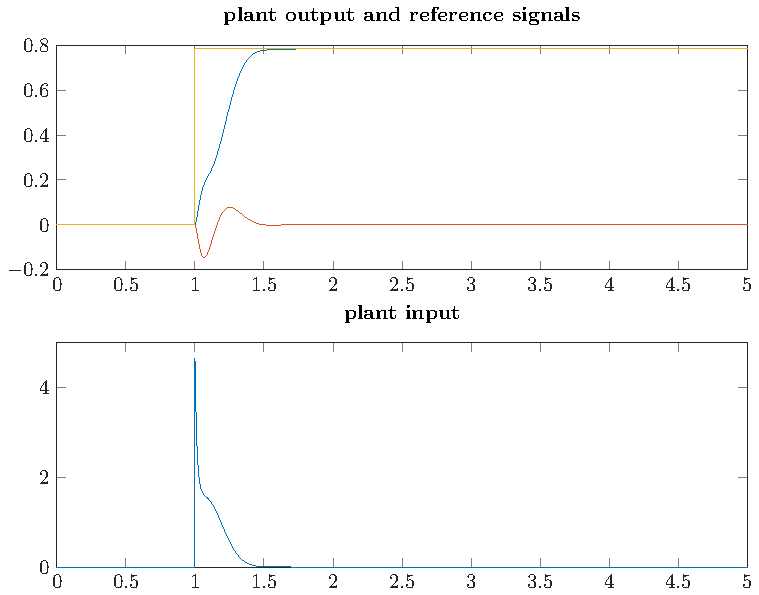
\includegraphics[scale=0.46]{images/orgFullState.pdf}
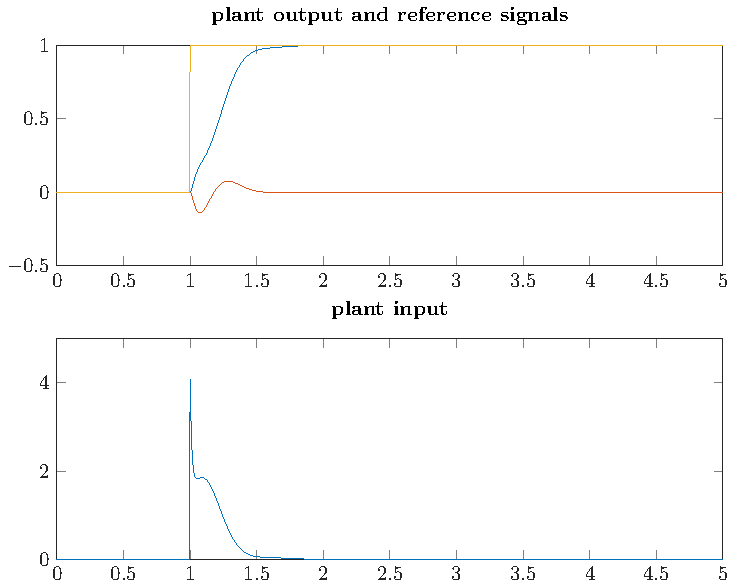
\includegraphics[scale=0.46]{images/optFullState.pdf}
\caption{Simulation results for the original weighting parameters left and for the improved weighting parameters right. Plant input is given in Volt [V]. Plant output and references are given in radians [rad].}
\label{fig:stepResponse}
\end{figure}


\section{Concluding Simulations with filter and differentiator}
\begin{figure}
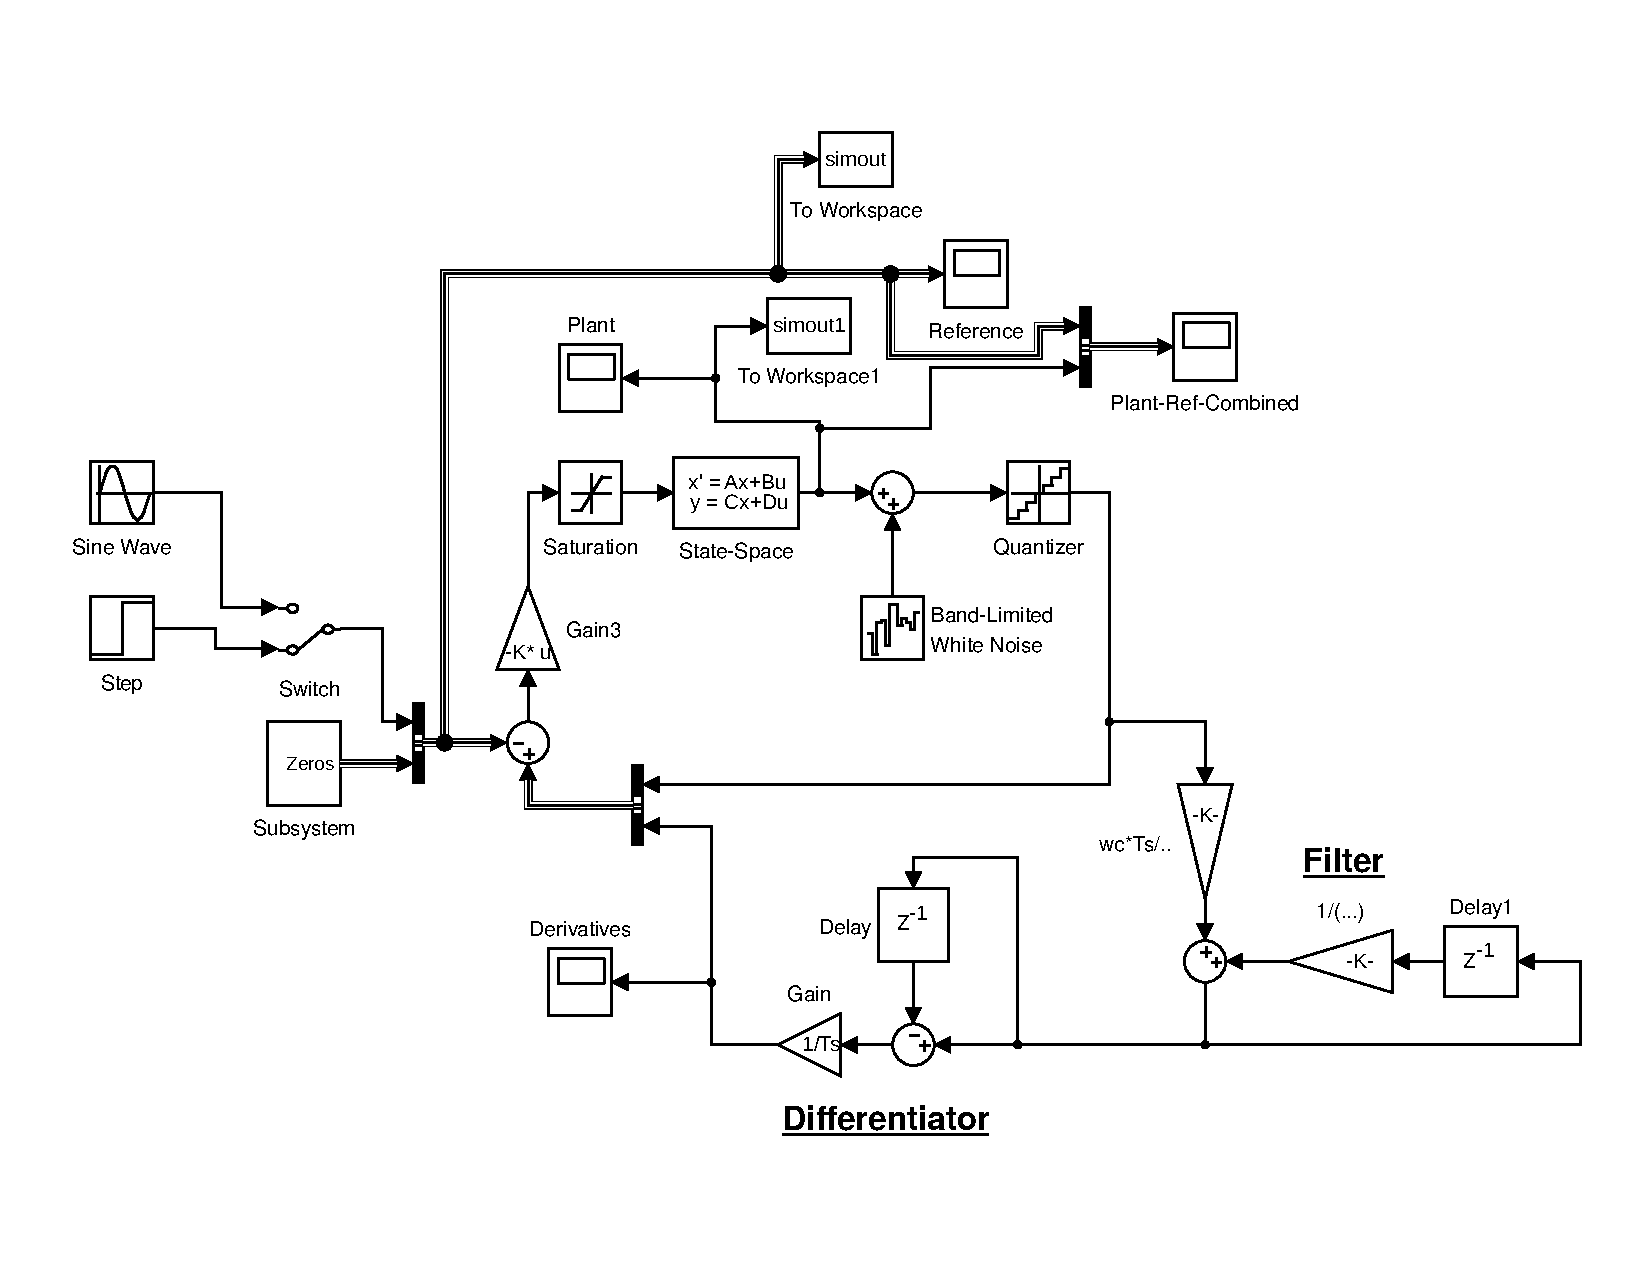
\includegraphics[scale=0.5]{images/simModel.pdf}
\caption{The simulink Layout of our Simulation}
\end{figure}



\chapter{Tests of the controller on the real setup}

\begin{figure} \label{realtimeSimDiagram}
  \centering
  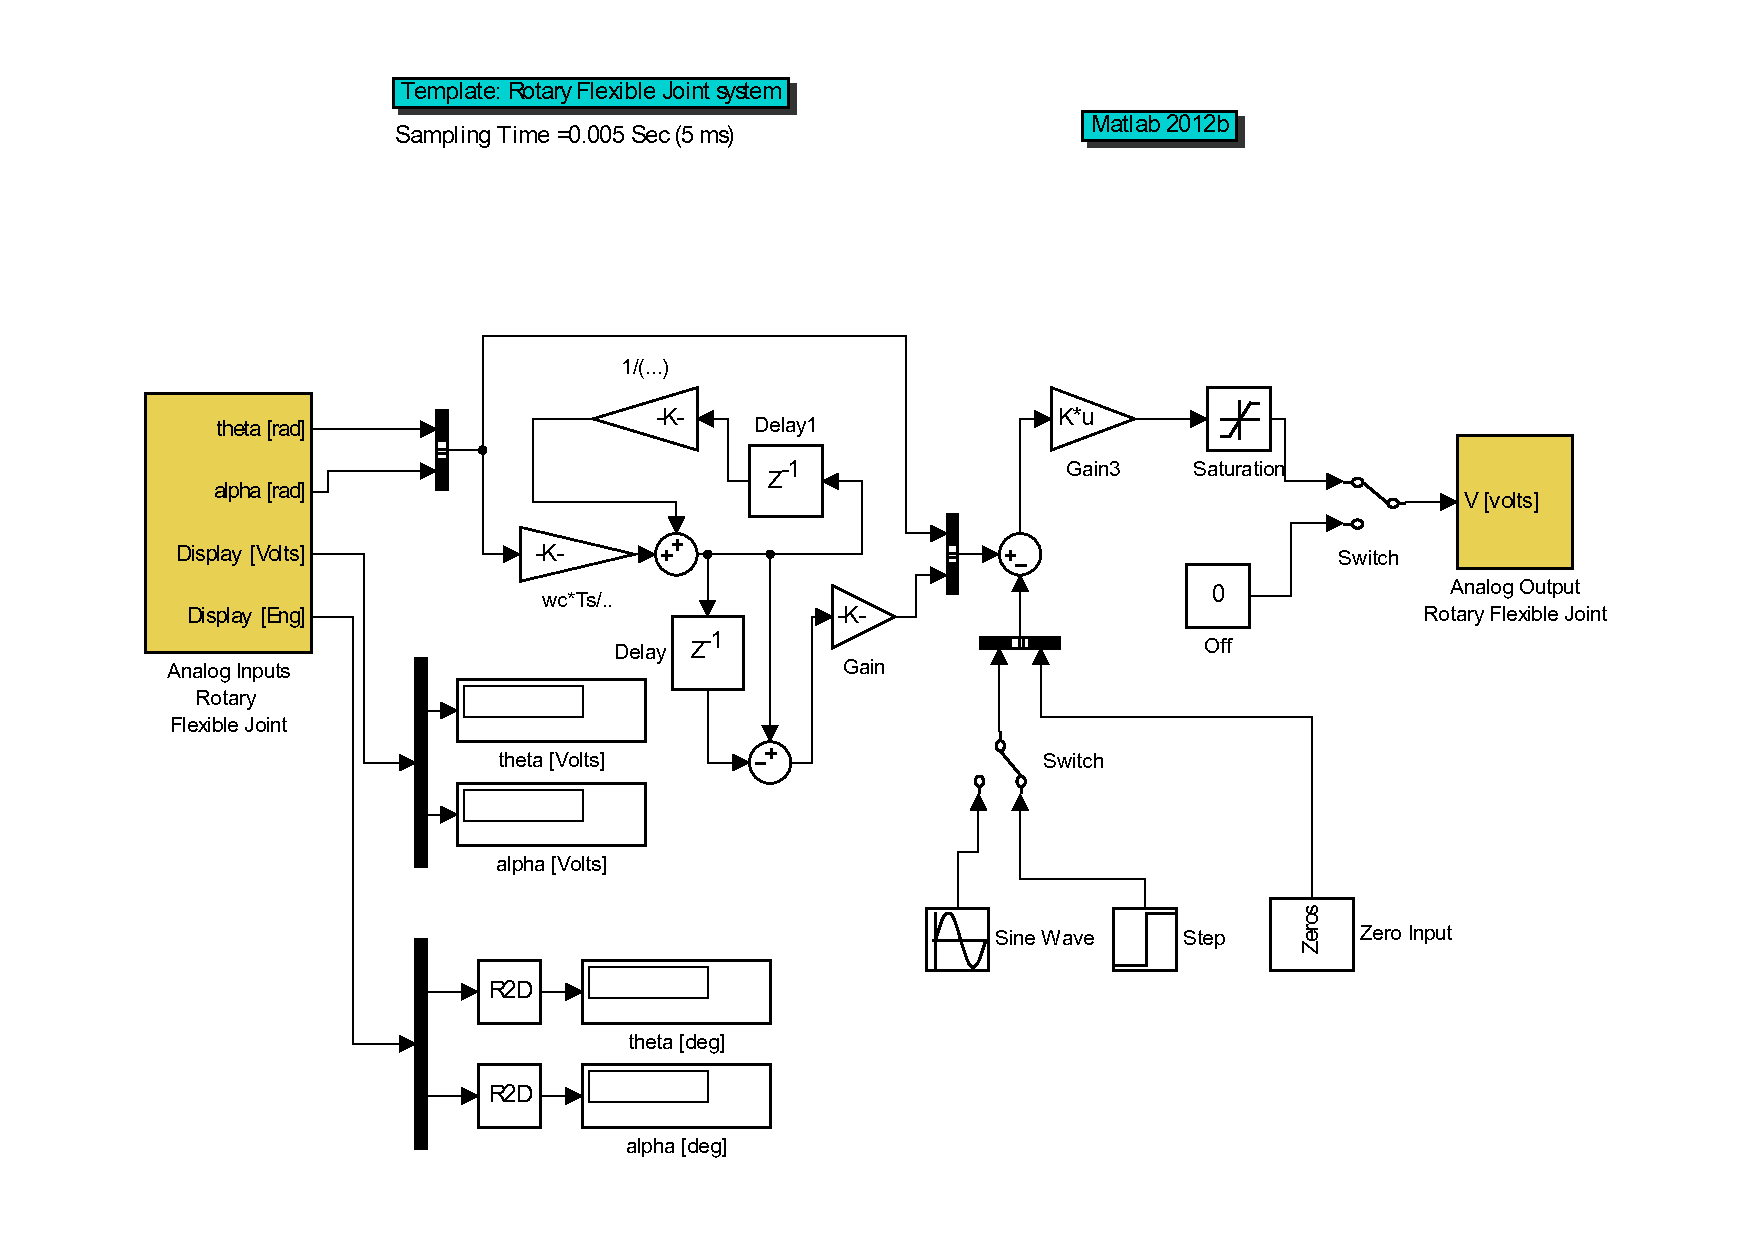
\includegraphics[scale=0.4]{images/realtimeSimDiagram}
  \caption{Real-time Simulink diagram} 
\end{figure}

In figure $\eqref{realtimeSimDiagram}$ we see the real-time Simulink diagram that we used in the lab to run our experiments on the real setup. The "Analog Input" block sends measurements of the sensors into the template. Each sensor reading is updated with a sampling time of 5 ms, in radians for the angles of the hub and arm. Additionally this block has two special outputs, "Display[volts]" and "Display[Eng]", which are used for visualization purposes. These two outputs are connected to a set of displays in order to provide a local visual measure of the process variables. 

The "Analog Output" block allows the controller to send a voltage signal to the motor of the hub. At the input of this block there is an on-off switch. This switch allows the user to switch the motor on or off. We included a saturator in our diagram just before the signal goes in to the "Analog Output" to limit the control input within $-5V$ and $5V$. The saturation settings of the block in our diagram are set accordingly. We also included a sine wave, a step input and a zero input. These two block are used as a reference for $\theta_{desired}$. The zero block contains 3 signals equal to zero that represent the references for $\alpha, \dot{\theta}$ and $\dot{\alpha}$.


\section{Setpoint tracking}
\begin{figure}
%If time later use these and adjust size in .tex file.
%% This file was created by matlab2tikz v0.4.7 running on MATLAB 8.4.
% Copyright (c) 2008--2014, Nico Schlömer <nico.schloemer@gmail.com>
% All rights reserved.
% Minimal pgfplots version: 1.3
% 
% The latest updates can be retrieved from
%   http://www.mathworks.com/matlabcentral/fileexchange/22022-matlab2tikz
% where you can also make suggestions and rate matlab2tikz.
% 
\documentclass[tikz]{standalone}
\usepackage{pgfplots}
\usepackage{grffile}
\pgfplotsset{compat=newest}
\usetikzlibrary{plotmarks}
\usepackage{amsmath}

\begin{document}
%
% defining custom colors
\definecolor{mycolor1}{rgb}{0.00000,0.44700,0.74100}%
\definecolor{mycolor2}{rgb}{0.85000,0.32500,0.09800}%
\definecolor{mycolor3}{rgb}{0.92900,0.69400,0.12500}%
%
\begin{tikzpicture}

\begin{axis}[%
width=2in,
height=1in,
scale only axis,
separate axis lines,
every outer x axis line/.append style={white!15!black},
every x tick label/.append style={font=\color{white!15!black}},
xmin=0,
xmax=7,
xmajorgrids,
every outer y axis line/.append style={white!15!black},
every y tick label/.append style={font=\color{white!15!black}},
ymin=-20,
ymax=60,
ymajorgrids,
name=plot1,
title style={font=\bfseries},
ylabel={reference, plant [$\;^\circ$]}
]
\addplot [color=mycolor1,solid,forget plot]
  table[row sep=crcr]{0	-1.81449008178188\\
0.005	-1.75197319638422\\
0.01	-1.78323163908305\\
0.015	-1.84574852448072\\
0.02	-1.83532904358111\\
0.025	-1.75197319638422\\
0.03	-1.80407060088227\\
0.035	-1.84574852448072\\
0.04	-1.77281215818344\\
0.045	-1.68945631098655\\
0.05	-1.68945631098655\\
0.055	-1.77281215818344\\
0.06	-1.73113423458499\\
0.065	-1.64777838738811\\
0.07	-1.65819786828772\\
0.075	-1.74155371548461\\
0.08	-1.67903683008694\\
0.085	-1.54358357839199\\
0.09	-1.56442254019122\\
0.095	-1.65819786828772\\
0.1	-1.60610046378966\\
0.105	-1.50190565479355\\
0.11	-1.54358357839199\\
0.115	-1.60610046378966\\
0.12	-1.56442254019122\\
0.125	-1.43938876939588\\
0.13	-1.4602277311951\\
0.135	-1.52274461659277\\
0.14	-1.48106669299433\\
0.145	-1.40813032669705\\
0.15	-1.38729136489783\\
0.155	-1.48106669299433\\
0.16	-1.43938876939588\\
0.165	-1.3664524030986\\
0.17	-1.38729136489783\\
0.175	-1.48106669299433\\
0.18	-1.42896928849627\\
0.185	-1.34561344129938\\
0.19	-1.33519396039977\\
0.195	-1.42896928849627\\
0.2	-1.39771084579744\\
0.205	-1.31435499860055\\
0.21	-1.33519396039977\\
0.215	-1.43938876939588\\
0.22	-1.42896928849627\\
0.225	-1.33519396039977\\
0.23	-1.34561344129938\\
0.235	-1.42896928849627\\
0.24	-1.41854980759666\\
0.245	-1.30393551770094\\
0.25	-1.34561344129938\\
0.255	-1.42896928849627\\
0.26	-1.41854980759666\\
0.265	-1.33519396039977\\
0.27	-1.33519396039977\\
0.275	-1.43938876939588\\
0.28	-1.44980825029549\\
0.285	-1.30393551770094\\
0.29	-1.32477447950016\\
0.295	-1.42896928849627\\
0.3	-1.40813032669705\\
0.305	-1.32477447950016\\
0.31	-1.32477447950016\\
0.315	-1.42896928849627\\
0.32	-1.41854980759666\\
0.325	-1.31435499860055\\
0.33	-1.3664524030986\\
0.335	-1.39771084579744\\
0.34	-1.41854980759666\\
0.345	-1.29351603680133\\
0.35	-1.35603292219899\\
0.355	-1.42896928849627\\
0.36	-1.41854980759666\\
0.365	-1.32477447950016\\
0.37	-1.34561344129938\\
0.375	-1.43938876939588\\
0.38	-1.42896928849627\\
0.385	-1.33519396039977\\
0.39	-1.33519396039977\\
0.395	-1.41854980759666\\
0.4	-1.42896928849627\\
0.405	-1.32477447950016\\
0.41	-1.35603292219899\\
0.415	-1.43938876939588\\
0.42	-1.40813032669705\\
0.425	-1.32477447950016\\
0.43	-1.33519396039977\\
0.435	-1.42896928849627\\
0.44	-1.40813032669705\\
0.445	-1.31435499860055\\
0.45	-1.3664524030986\\
0.455	-1.43938876939588\\
0.46	-1.41854980759666\\
0.465	-1.32477447950016\\
0.47	-1.34561344129938\\
0.475	-1.43938876939588\\
0.48	-1.40813032669705\\
0.485	-1.31435499860055\\
0.49	-1.35603292219899\\
0.495	-1.42896928849627\\
0.5	-1.39771084579744\\
0.505	-1.30393551770094\\
0.51	-1.34561344129938\\
0.515	-1.42896928849627\\
0.52	-1.41854980759666\\
0.525	-1.34561344129938\\
0.53	-1.32477447950016\\
0.535	-1.44980825029549\\
0.54	-1.42896928849627\\
0.545	-1.32477447950016\\
0.55	-1.35603292219899\\
0.555	-1.42896928849627\\
0.56	-1.40813032669705\\
0.565	-1.32477447950016\\
0.57	-1.33519396039977\\
0.575	-1.44980825029549\\
0.58	-1.42896928849627\\
0.585	-1.33519396039977\\
0.59	-1.32477447950016\\
0.595	-1.42896928849627\\
0.6	-1.40813032669705\\
0.605	-1.32477447950016\\
0.61	-1.37687188399822\\
0.615	-1.42896928849627\\
0.62	-1.40813032669705\\
0.625	-1.31435499860055\\
0.63	-1.34561344129938\\
0.635	-1.44980825029549\\
0.64	-1.40813032669705\\
0.645	-1.31435499860055\\
0.65	-1.33519396039977\\
0.655	-1.41854980759666\\
0.66	-1.42896928849627\\
0.665	-1.30393551770094\\
0.67	-1.35603292219899\\
0.675	-1.43938876939588\\
0.68	-1.40813032669705\\
0.685	-1.32477447950016\\
0.69	-1.3664524030986\\
0.695	-1.42896928849627\\
0.7	-1.40813032669705\\
0.705	-1.33519396039977\\
0.71	-1.33519396039977\\
0.715	-1.41854980759666\\
0.72	-1.40813032669705\\
0.725	-1.32477447950016\\
0.73	-1.33519396039977\\
0.735	-1.41854980759666\\
0.74	-1.41854980759666\\
0.745	-1.31435499860055\\
0.75	-1.35603292219899\\
0.755	-1.42896928849627\\
0.76	-1.41854980759666\\
0.765	-1.30393551770094\\
0.77	-1.35603292219899\\
0.775	-1.41854980759666\\
0.78	-1.40813032669705\\
0.785	-1.30393551770094\\
0.79	-1.32477447950016\\
0.795	-1.42896928849627\\
0.8	-1.43938876939588\\
0.805	-1.32477447950016\\
0.81	-1.34561344129938\\
0.815	-1.43938876939588\\
0.82	-1.41854980759666\\
0.825	-1.31435499860055\\
0.83	-1.33519396039977\\
0.835	-1.41854980759666\\
0.84	-1.41854980759666\\
0.845	-1.32477447950016\\
0.85	-1.31435499860055\\
0.855	-1.39771084579744\\
0.86	-1.40813032669705\\
0.865	-1.33519396039977\\
0.87	-1.30393551770094\\
0.875	-1.43938876939588\\
0.88	-1.42896928849627\\
0.885	-1.33519396039977\\
0.89	-1.32477447950016\\
0.895	-1.41854980759666\\
0.9	-1.41854980759666\\
0.905	-1.33519396039977\\
0.91	-1.33519396039977\\
0.915	-1.40813032669705\\
0.92	-1.39771084579744\\
0.925	-1.31435499860055\\
0.93	-1.32477447950016\\
0.935	-1.42896928849627\\
0.94	-1.41854980759666\\
0.945	-1.33519396039977\\
0.95	-1.32477447950016\\
0.955	-1.40813032669705\\
0.96	-1.41854980759666\\
0.965	-1.31435499860055\\
0.97	-1.32477447950016\\
0.975	-1.42896928849627\\
0.98	-1.39771084579744\\
0.985	-1.31435499860055\\
0.99	-1.33519396039977\\
0.995	-1.41854980759666\\
1	-1.40813032669705\\
1.005	-1.91868489077799\\
1.01	-1.47064721209472\\
1.015	-0.86631731991727\\
1.02	-0.147373137844102\\
1.025	0.759121700422066\\
1.03	1.62393861508979\\
1.035	2.30120487356451\\
1.04	3.1347633455334\\
1.045	3.96832181750229\\
1.05	4.61432963327819\\
1.055	5.05194783106185\\
1.06	5.48956602884552\\
1.065	5.98970111202685\\
1.07	6.32312450081441\\
1.075	6.53151411880663\\
1.08	6.83367906489536\\
1.085	7.20878037728136\\
1.09	7.54220376606891\\
1.095	7.76101286496075\\
1.1	8.02149988745103\\
1.105	8.4695375661343\\
1.11	8.8446388785203\\
1.115	9.09470642011097\\
1.12	9.48022721339658\\
1.125	10.0428791819756\\
1.13	10.4492389370604\\
1.135	10.8764376539445\\
1.14	11.397411698925\\
1.145	12.0642584765001\\
1.15	12.7311052540753\\
1.155	13.2520792990558\\
1.16	13.9085065957313\\
1.165	14.6899676632022\\
1.17	15.3776534025765\\
1.175	16.0028222565531\\
1.18	16.7426054004255\\
1.185	17.5970028341937\\
1.19	18.336785978066\\
1.195	18.9619548320427\\
1.2	19.5767042051198\\
1.205	20.2852289062933\\
1.21	20.9312367220692\\
1.215	21.4209523243509\\
1.22	22.035701697428\\
1.225	22.7338069177019\\
1.23	23.3381368098794\\
1.235	23.8070134503619\\
1.24	24.3384069762421\\
1.245	24.9114784257207\\
1.25	25.4324524707012\\
1.255	25.8492317066857\\
1.26	26.3597862707666\\
1.265	26.9953746056429\\
1.27	27.5267681315231\\
1.275	27.9227084057083\\
1.28	28.3811655652912\\
1.285	28.9542370147698\\
1.29	29.3605967698546\\
1.295	29.7565370440398\\
1.3	30.1524773182251\\
1.305	30.6838708441052\\
1.31	31.0798111182905\\
1.315	31.36113710258\\
1.32	31.6841410104679\\
1.325	32.1946955745489\\
1.33	32.4656020779387\\
1.335	32.6635722150314\\
1.34	32.9240592375216\\
1.345	33.288741069008\\
1.35	33.5283891296991\\
1.355	33.6534229004944\\
1.36	33.9139099229847\\
1.365	34.226494349973\\
1.37	34.414045006166\\
1.375	34.5078203342625\\
1.38	34.6641125477567\\
1.385	34.9662774938454\\
1.39	35.1746671118376\\
1.395	35.2892814017334\\
1.4	35.4768320579264\\
1.405	35.7789970040151\\
1.41	35.9457086984089\\
1.415	36.0082255838065\\
1.42	36.1436788355015\\
1.425	36.4041658579917\\
1.43	36.5291996287871\\
1.435	36.5396191096867\\
1.44	36.6854918422813\\
1.445	36.852203536675\\
1.45	36.9668178265707\\
1.455	36.9668178265707\\
1.46	37.0501736737676\\
1.465	37.2377243299606\\
1.47	37.2481438108602\\
1.475	37.2064658872618\\
1.48	37.2377243299606\\
1.485	37.3314996580571\\
1.49	37.3940165434548\\
1.495	37.3314996580571\\
1.5	37.4044360243544\\
1.505	37.5294697951498\\
1.51	37.5919866805474\\
1.515	37.550308756949\\
1.52	37.5919866805474\\
1.525	37.7586983749412\\
1.53	37.8107957794393\\
1.535	37.737859413142\\
1.54	37.8003762985396\\
1.545	37.9358295502346\\
1.55	37.9670879929334\\
1.555	37.9045711075357\\
1.56	37.9149905884354\\
1.565	38.0296048783311\\
1.57	38.0712828019295\\
1.575	37.977507473833\\
1.58	38.0296048783311\\
1.585	38.1442191682268\\
1.59	38.1963165727249\\
1.595	38.1546386491264\\
1.6	38.1858970918252\\
1.605	38.300511381721\\
1.61	38.352608786219\\
1.615	38.300511381721\\
1.62	38.352608786219\\
1.625	38.5089009997132\\
1.63	38.5714178851109\\
1.635	38.5089009997132\\
1.64	38.5297399615124\\
1.645	38.6860321750066\\
1.65	38.727710098605\\
1.655	38.6339347705085\\
1.66	38.6964516559062\\
1.665	38.8527438694004\\
1.67	38.9360997165973\\
1.675	38.8840023120992\\
1.68	38.9256802356976\\
1.685	39.0715529682922\\
1.69	39.1340698536899\\
1.695	39.0819724491918\\
1.7	39.1132308918906\\
1.705	39.2486841435856\\
1.71	39.3320399907825\\
1.715	39.2695231053848\\
1.72	39.3007815480836\\
1.725	39.4674932424774\\
1.73	39.5091711660759\\
1.735	39.4674932424774\\
1.74	39.4987516851763\\
1.745	39.6446244177708\\
1.75	39.6758828604696\\
1.755	39.6550438986704\\
1.76	39.6758828604696\\
1.765	39.8321750739638\\
1.77	39.8634335166626\\
1.775	39.8217555930642\\
1.78	39.8217555930642\\
1.785	39.9676283256588\\
1.79	40.0509841728556\\
1.795	39.9572088447591\\
1.8	39.9467893638595\\
1.805	40.0926620964541\\
1.81	40.1551789818518\\
1.815	40.040564691956\\
1.82	40.0509841728556\\
1.825	40.1864374245506\\
1.83	40.2385348290486\\
1.835	40.1655984627514\\
1.84	40.176017943651\\
1.845	40.3010517144463\\
1.85	40.3218906762455\\
1.855	40.2489543099483\\
1.86	40.228115348149\\
1.865	40.3948270425428\\
1.87	40.4573439279405\\
1.875	40.3531491189444\\
1.88	40.3531491189444\\
1.885	40.4886023706393\\
1.89	40.5302802942378\\
1.895	40.4573439279405\\
1.9	40.4677634088401\\
1.905	40.6136361414346\\
1.91	40.6240556223343\\
1.915	40.5615387369366\\
1.92	40.551119256037\\
1.925	40.6657335459327\\
1.93	40.6969919886315\\
1.935	40.6136361414346\\
1.94	40.6344751032339\\
1.945	40.7595088740292\\
1.95	40.8011867976276\\
1.955	40.6969919886315\\
1.96	40.7074114695311\\
1.965	40.8220257594269\\
1.97	40.8741231639249\\
1.975	40.790767316728\\
1.98	40.8116062785273\\
1.985	40.926220568423\\
1.99	40.9470595302222\\
1.995	40.8949621257241\\
2	40.9158010875234\\
2.005	40.9991569347203\\
2.01	41.0616738201179\\
2.015	40.978317972921\\
2.02	40.9678984920214\\
2.025	41.0929322628168\\
2.03	41.1241907055156\\
2.035	41.0095764156199\\
2.04	41.0304153774191\\
2.045	41.165868629114\\
2.05	41.1971270718129\\
2.055	41.1033517437164\\
2.06	41.0929322628168\\
2.065	41.2283855145117\\
2.07	41.2804829190098\\
2.075	41.1867075909133\\
2.08	41.1554491482144\\
2.085	41.301321880809\\
2.09	41.3429998044074\\
2.095	41.2388049954113\\
2.1	41.2492244763109\\
2.105	41.353419285307\\
2.11	41.353419285307\\
2.115	41.2909023999094\\
2.12	41.2700634381101\\
2.125	41.3846777280059\\
2.13	41.4159361707047\\
2.135	41.3117413617086\\
2.14	41.3117413617086\\
2.145	41.4159361707047\\
2.15	41.4680335752028\\
2.155	41.3742582471063\\
2.16	41.3429998044074\\
2.165	41.4576140943031\\
2.17	41.5305504606004\\
2.175	41.4055166898051\\
2.18	41.3950972089055\\
2.185	41.5201309797008\\
2.19	41.5513894223996\\
2.195	41.4576140943031\\
2.2	41.4055166898051\\
2.205	41.5409699415\\
2.21	41.5722283841989\\
2.215	41.4784530561024\\
2.22	41.4471946134035\\
2.225	41.5826478650985\\
2.23	41.6139063077973\\
2.235	41.5097114988012\\
2.24	41.488872537002\\
2.245	41.5930673459981\\
2.25	41.6347452695965\\
2.255	41.4992920179016\\
2.26	41.4784530561024\\
2.265	41.5722283841989\\
2.27	41.6034868268977\\
2.275	41.5097114988012\\
2.28	41.4784530561024\\
2.285	41.5722283841989\\
2.29	41.5930673459981\\
2.295	41.5305504606004\\
2.3	41.488872537002\\
2.305	41.6139063077973\\
2.31	41.5930673459981\\
2.315	41.4992920179016\\
2.32	41.5097114988012\\
2.325	41.6347452695965\\
2.33	41.6451647504961\\
2.335	41.5513894223996\\
2.34	41.5305504606004\\
2.345	41.6451647504961\\
2.35	41.6868426740946\\
2.355	41.5826478650985\\
2.36	41.5305504606004\\
2.365	41.6451647504961\\
2.37	41.676423193195\\
2.375	41.5826478650985\\
2.38	41.5409699415\\
2.385	41.676423193195\\
2.39	41.6868426740946\\
2.395	41.6139063077973\\
2.4	41.5722283841989\\
2.405	41.6972621549942\\
2.41	41.7493595594923\\
2.415	41.6660037122954\\
2.42	41.6034868268977\\
2.425	41.7181011167934\\
2.43	41.7597790403919\\
2.435	41.6451647504961\\
2.44	41.6347452695965\\
2.445	41.7493595594923\\
2.45	41.7701985212915\\
2.455	41.6972621549942\\
2.46	41.676423193195\\
2.465	41.7806180021911\\
2.47	41.8327154066891\\
2.475	41.7181011167934\\
2.48	41.7181011167934\\
2.485	41.8014569639903\\
2.49	41.8535543684884\\
2.495	41.7806180021911\\
2.5	41.7389400785926\\
2.505	41.8431348875888\\
2.51	41.863973849388\\
2.515	41.7806180021911\\
2.52	41.7181011167934\\
2.525	41.863973849388\\
2.53	41.8848128111872\\
2.535	41.7910374830907\\
2.54	41.7701985212915\\
2.545	41.8743933302876\\
2.55	41.9369102156853\\
2.555	41.8014569639903\\
2.56	41.7910374830907\\
2.565	41.863973849388\\
2.57	41.9369102156853\\
2.575	41.8222959257895\\
2.58	41.8014569639903\\
2.585	41.9264907347857\\
2.59	41.9473296965849\\
2.595	41.8535543684884\\
2.6	41.7806180021911\\
2.605	41.8952322920868\\
2.61	41.9369102156853\\
2.615	41.8327154066891\\
2.62	41.8327154066891\\
2.625	41.9369102156853\\
2.63	41.9890076201833\\
2.635	41.8431348875888\\
2.64	41.8222959257895\\
2.645	41.9681686583841\\
2.65	41.9785881392837\\
2.655	41.8535543684884\\
2.66	41.8014569639903\\
2.665	41.9056517729864\\
2.67	41.9577491774845\\
2.675	41.8535543684884\\
2.68	41.8014569639903\\
2.685	41.9056517729864\\
2.69	41.9681686583841\\
2.695	41.8535543684884\\
2.7	41.8014569639903\\
2.705	41.9264907347857\\
2.71	41.9473296965849\\
2.715	41.8535543684884\\
2.72	41.8118764448899\\
2.725	41.9369102156853\\
2.73	41.9785881392837\\
2.735	41.8848128111872\\
2.74	41.8222959257895\\
2.745	41.9264907347857\\
2.75	41.9890076201833\\
2.755	41.8743933302876\\
2.76	41.8431348875888\\
2.765	41.9473296965849\\
2.77	41.9785881392837\\
2.775	41.8848128111872\\
2.78	41.8327154066891\\
2.785	41.9473296965849\\
2.79	41.9577491774845\\
2.795	41.8743933302876\\
2.8	41.8327154066891\\
2.805	41.9473296965849\\
2.81	41.9890076201833\\
2.815	41.8848128111872\\
2.82	41.8535543684884\\
2.825	41.9681686583841\\
2.83	42.0098465819825\\
2.835	41.8952322920868\\
2.84	41.8743933302876\\
2.845	41.9473296965849\\
2.85	41.9890076201833\\
2.855	41.8952322920868\\
2.86	41.863973849388\\
2.865	41.9577491774845\\
2.87	42.0098465819825\\
2.875	41.916071253886\\
2.88	41.8743933302876\\
2.885	41.9785881392837\\
2.89	42.0098465819825\\
2.895	41.916071253886\\
2.9	41.863973849388\\
2.905	41.9577491774845\\
2.91	42.0202660628821\\
2.915	41.9369102156853\\
2.92	41.8952322920868\\
2.925	41.9994271010829\\
2.93	42.0619439864806\\
2.935	41.9369102156853\\
2.94	41.8743933302876\\
2.945	41.9785881392837\\
2.95	42.0411050246814\\
2.955	41.9473296965849\\
2.96	41.8848128111872\\
2.965	41.9785881392837\\
2.97	42.0306855437818\\
2.975	41.9369102156853\\
2.98	41.8743933302876\\
2.985	42.0098465819825\\
2.99	42.051524505581\\
2.995	41.9369102156853\\
3	41.916071253886\\
3.005	41.9994271010829\\
3.01	42.0619439864806\\
3.015	41.9577491774845\\
3.02	41.9264907347857\\
3.025	42.0098465819825\\
3.03	42.0619439864806\\
3.035	41.9681686583841\\
3.04	41.916071253886\\
3.045	42.0619439864806\\
3.05	42.0723634673802\\
3.055	41.9890076201833\\
3.06	41.9264907347857\\
3.065	42.0098465819825\\
3.07	42.051524505581\\
3.075	41.9785881392837\\
3.08	41.9369102156853\\
3.085	42.0202660628821\\
3.09	42.0827829482798\\
3.095	41.9890076201833\\
3.1	41.9577491774845\\
3.105	42.0619439864806\\
3.11	42.0827829482798\\
3.115	41.9785881392837\\
3.12	41.9473296965849\\
3.125	42.0411050246814\\
3.13	42.0827829482798\\
3.135	42.0306855437818\\
3.14	41.9473296965849\\
3.145	42.0619439864806\\
3.15	42.1244608718783\\
3.155	42.0098465819825\\
3.16	41.9681686583841\\
3.165	42.0827829482798\\
3.17	42.1244608718783\\
3.175	41.9994271010829\\
3.18	41.9994271010829\\
3.185	42.0827829482798\\
3.19	42.1348803527779\\
3.195	42.0306855437818\\
3.2	41.9681686583841\\
3.205	42.0827829482798\\
3.21	42.1244608718783\\
3.215	42.0098465819825\\
3.22	41.9890076201833\\
3.225	42.103621910079\\
3.23	42.1557193145771\\
3.235	42.0098465819825\\
3.24	41.9890076201833\\
3.245	42.0723634673802\\
3.25	42.1348803527779\\
3.255	42.051524505581\\
3.26	42.0098465819825\\
3.265	42.1140413909786\\
3.27	42.1557193145771\\
3.275	42.0619439864806\\
3.28	42.0202660628821\\
3.285	42.0827829482798\\
3.29	42.1452998336775\\
3.295	42.0723634673802\\
3.3	41.9890076201833\\
3.305	42.0932024291794\\
3.31	42.1348803527779\\
3.315	42.0723634673802\\
3.32	42.0098465819825\\
3.325	42.1140413909786\\
3.33	42.1869777572759\\
3.335	42.0932024291794\\
3.34	42.0411050246814\\
3.345	42.1244608718783\\
3.35	42.1869777572759\\
3.355	42.0932024291794\\
3.36	42.0306855437818\\
3.365	42.1244608718783\\
3.37	42.1661387954767\\
3.375	42.0723634673802\\
3.38	42.051524505581\\
3.385	42.1244608718783\\
3.39	42.1973972381755\\
3.395	42.0619439864806\\
3.4	42.0306855437818\\
3.405	42.1452998336775\\
3.41	42.2078167190751\\
3.415	42.1140413909786\\
3.42	42.051524505581\\
3.425	42.1452998336775\\
3.43	42.2182361999748\\
3.435	42.1140413909786\\
3.44	42.0411050246814\\
3.445	42.1557193145771\\
3.45	42.2182361999748\\
3.455	42.103621910079\\
3.46	42.0306855437818\\
3.465	42.1557193145771\\
3.47	42.2078167190751\\
3.475	42.1140413909786\\
3.48	42.0827829482798\\
3.485	42.1557193145771\\
3.49	42.2078167190751\\
3.495	42.1348803527779\\
3.5	42.051524505581\\
3.505	42.1765582763763\\
3.51	42.2078167190751\\
3.515	42.1348803527779\\
3.52	42.0619439864806\\
3.525	42.1869777572759\\
3.53	42.239075161774\\
3.535	42.1244608718783\\
3.54	42.0619439864806\\
3.545	42.1765582763763\\
3.55	42.2286556808744\\
3.555	42.1661387954767\\
3.56	42.0827829482798\\
3.565	42.1765582763763\\
3.57	42.2494946426736\\
3.575	42.1661387954767\\
3.58	42.0827829482798\\
3.585	42.1869777572759\\
3.59	42.2494946426736\\
3.595	42.1557193145771\\
3.6	42.0827829482798\\
3.605	42.1869777572759\\
3.61	42.2703336044728\\
3.615	42.1765582763763\\
3.62	42.0619439864806\\
3.625	42.2286556808744\\
3.63	42.2703336044728\\
3.635	42.1452998336775\\
3.64	42.0932024291794\\
3.645	42.1869777572759\\
3.65	42.2494946426736\\
3.655	42.1557193145771\\
3.66	42.0827829482798\\
3.665	42.2182361999748\\
3.67	42.239075161774\\
3.675	42.1452998336775\\
3.68	42.1140413909786\\
3.685	42.2182361999748\\
3.69	42.2703336044728\\
3.695	42.1765582763763\\
3.7	42.0932024291794\\
3.705	42.1869777572759\\
3.71	42.2286556808744\\
3.715	42.1557193145771\\
3.72	42.0932024291794\\
3.725	42.2286556808744\\
3.73	42.2807530853724\\
3.735	42.1661387954767\\
3.74	42.1140413909786\\
3.745	42.2286556808744\\
3.75	42.2703336044728\\
3.755	42.1557193145771\\
3.76	42.103621910079\\
3.765	42.2286556808744\\
3.77	42.3015920471716\\
3.775	42.1348803527779\\
3.78	42.1244608718783\\
3.785	42.2182361999748\\
3.79	42.3015920471716\\
3.795	42.1869777572759\\
3.8	42.1140413909786\\
3.805	42.2286556808744\\
3.81	42.3015920471716\\
3.815	42.1973972381755\\
3.82	42.1348803527779\\
3.825	42.2182361999748\\
3.83	42.291172566272\\
3.835	42.1869777572759\\
3.84	42.1140413909786\\
3.845	42.2286556808744\\
3.85	42.3120115280713\\
3.855	42.1869777572759\\
3.86	42.1244608718783\\
3.865	42.2286556808744\\
3.87	42.3120115280713\\
3.875	42.1869777572759\\
3.88	42.1140413909786\\
3.885	42.2494946426736\\
3.89	42.3015920471716\\
3.895	42.1765582763763\\
3.9	42.1140413909786\\
3.905	42.2494946426736\\
3.91	42.291172566272\\
3.915	42.2078167190751\\
3.92	42.1348803527779\\
3.925	42.2286556808744\\
3.93	42.2807530853724\\
3.935	42.1869777572759\\
3.94	42.1348803527779\\
3.945	42.2182361999748\\
3.95	42.3120115280713\\
3.955	42.1973972381755\\
3.96	42.1244608718783\\
3.965	42.239075161774\\
3.97	42.3015920471716\\
3.975	42.1869777572759\\
3.98	42.1452998336775\\
3.985	42.2494946426736\\
3.99	42.291172566272\\
3.995	42.1765582763763\\
4	42.1244608718783\\
4.005	42.2182361999748\\
4.01	42.3015920471716\\
4.015	42.1869777572759\\
4.02	42.1140413909786\\
4.025	42.2494946426736\\
4.03	42.3120115280713\\
4.035	42.1973972381755\\
4.04	42.1244608718783\\
4.045	42.2286556808744\\
4.05	42.3120115280713\\
4.055	42.1869777572759\\
4.06	42.1348803527779\\
4.065	42.239075161774\\
4.07	42.3328504898705\\
4.075	42.2078167190751\\
4.08	42.1348803527779\\
4.085	42.2703336044728\\
4.09	42.3224310089709\\
4.095	42.1973972381755\\
4.1	42.1557193145771\\
4.105	42.2286556808744\\
4.11	42.3328504898705\\
4.115	42.2182361999748\\
4.12	42.1244608718783\\
4.125	42.2494946426736\\
4.13	42.3120115280713\\
4.135	42.2182361999748\\
4.14	42.1557193145771\\
4.145	42.2599141235732\\
4.15	42.3120115280713\\
4.155	42.2286556808744\\
4.16	42.1557193145771\\
4.165	42.2494946426736\\
4.17	42.3432699707701\\
4.175	42.1973972381755\\
4.18	42.1557193145771\\
4.185	42.239075161774\\
4.19	42.3432699707701\\
4.195	42.2078167190751\\
4.2	42.1244608718783\\
4.205	42.2494946426736\\
4.21	42.3328504898705\\
4.215	42.2182361999748\\
4.22	42.1348803527779\\
4.225	42.2807530853724\\
4.23	42.3015920471716\\
4.235	42.2182361999748\\
4.24	42.1452998336775\\
4.245	42.239075161774\\
4.25	42.3120115280713\\
4.255	42.1973972381755\\
4.26	42.1140413909786\\
4.265	42.2599141235732\\
4.27	42.3120115280713\\
4.275	42.2182361999748\\
4.28	42.1452998336775\\
4.285	42.239075161774\\
4.29	42.3120115280713\\
4.295	42.2182361999748\\
4.3	42.1452998336775\\
4.305	42.2599141235732\\
4.31	42.3120115280713\\
4.315	42.2078167190751\\
4.32	42.1452998336775\\
4.325	42.239075161774\\
4.33	42.3120115280713\\
4.335	42.2182361999748\\
4.34	42.1557193145771\\
4.345	42.2599141235732\\
4.35	42.3224310089709\\
4.355	42.2286556808744\\
4.36	42.1765582763763\\
4.365	42.2703336044728\\
4.37	42.3328504898705\\
4.375	42.2286556808744\\
4.38	42.1244608718783\\
4.385	42.2703336044728\\
4.39	42.3120115280713\\
4.395	42.2182361999748\\
4.4	42.1557193145771\\
4.405	42.2599141235732\\
4.41	42.3224310089709\\
4.415	42.2286556808744\\
4.42	42.1765582763763\\
4.425	42.2807530853724\\
4.43	42.3120115280713\\
4.435	42.2182361999748\\
4.44	42.1452998336775\\
4.445	42.2703336044728\\
4.45	42.3536894516697\\
4.455	42.239075161774\\
4.46	42.1869777572759\\
4.465	42.2703336044728\\
4.47	42.3432699707701\\
4.475	42.2286556808744\\
4.48	42.1348803527779\\
4.485	42.2703336044728\\
4.49	42.3328504898705\\
4.495	42.239075161774\\
4.5	42.1557193145771\\
4.505	42.2807530853724\\
4.51	42.3432699707701\\
4.515	42.2182361999748\\
4.52	42.1765582763763\\
4.525	42.2807530853724\\
4.53	42.3328504898705\\
4.535	42.2286556808744\\
4.54	42.1765582763763\\
4.545	42.291172566272\\
4.55	42.3641089325693\\
4.555	42.2286556808744\\
4.56	42.1765582763763\\
4.565	42.3015920471716\\
4.57	42.3224310089709\\
4.575	42.239075161774\\
4.58	42.1557193145771\\
4.585	42.2703336044728\\
4.59	42.3432699707701\\
4.595	42.239075161774\\
4.6	42.1765582763763\\
4.605	42.2599141235732\\
4.61	42.3432699707701\\
4.615	42.2182361999748\\
4.62	42.1557193145771\\
4.625	42.2599141235732\\
4.63	42.3120115280713\\
4.635	42.2286556808744\\
4.64	42.1765582763763\\
4.645	42.2807530853724\\
4.65	42.3432699707701\\
4.655	42.2494946426736\\
4.66	42.1765582763763\\
4.665	42.2807530853724\\
4.67	42.3641089325693\\
4.675	42.2286556808744\\
4.68	42.1557193145771\\
4.685	42.291172566272\\
4.69	42.3536894516697\\
4.695	42.2599141235732\\
4.7	42.1765582763763\\
4.705	42.3015920471716\\
4.71	42.3328504898705\\
4.715	42.2494946426736\\
4.72	42.1869777572759\\
4.725	42.2703336044728\\
4.73	42.3536894516697\\
4.735	42.239075161774\\
4.74	42.1661387954767\\
4.745	42.2807530853724\\
4.75	42.3641089325693\\
4.755	42.239075161774\\
4.76	42.1557193145771\\
4.765	42.2807530853724\\
4.77	42.3745284134689\\
4.775	42.239075161774\\
4.78	42.1557193145771\\
4.785	42.2599141235732\\
4.79	42.3224310089709\\
4.795	42.2286556808744\\
4.8	42.1765582763763\\
4.805	42.291172566272\\
4.81	42.3328504898705\\
4.815	42.2599141235732\\
4.82	42.1765582763763\\
4.825	42.2807530853724\\
4.83	42.3536894516697\\
4.835	42.2494946426736\\
4.84	42.1973972381755\\
4.845	42.2703336044728\\
4.85	42.3641089325693\\
4.855	42.2599141235732\\
4.86	42.1661387954767\\
4.865	42.3120115280713\\
4.87	42.3536894516697\\
4.875	42.239075161774\\
4.88	42.1661387954767\\
4.885	42.2703336044728\\
4.89	42.3536894516697\\
4.895	42.2494946426736\\
4.9	42.1765582763763\\
4.905	42.3120115280713\\
4.91	42.3745284134689\\
4.915	42.2703336044728\\
4.92	42.1869777572759\\
4.925	42.3015920471716\\
4.93	42.3849478943685\\
4.935	42.239075161774\\
4.94	42.1661387954767\\
4.945	42.291172566272\\
4.95	42.3432699707701\\
4.955	42.2494946426736\\
4.96	42.1765582763763\\
4.965	42.3015920471716\\
4.97	42.3432699707701\\
4.975	42.239075161774\\
4.98	42.1765582763763\\
4.985	42.3224310089709\\
4.99	42.3432699707701\\
4.995	42.2599141235732\\
5	42.1869777572759\\
5.005	42.3015920471716\\
5.01	42.3745284134689\\
5.015	42.2599141235732\\
5.02	42.1973972381755\\
5.025	42.291172566272\\
5.03	42.3641089325693\\
5.035	42.239075161774\\
5.04	42.1869777572759\\
5.045	42.3224310089709\\
5.05	42.3745284134689\\
5.055	42.2807530853724\\
5.06	42.1869777572759\\
5.065	42.3015920471716\\
5.07	42.3745284134689\\
5.075	42.2703336044728\\
5.08	42.2182361999748\\
5.085	42.3120115280713\\
5.09	42.3745284134689\\
5.095	42.2599141235732\\
5.1	42.1765582763763\\
5.105	42.3328504898705\\
5.11	42.3641089325693\\
5.115	42.2599141235732\\
5.12	42.1869777572759\\
5.125	42.291172566272\\
5.13	42.3849478943685\\
5.135	42.2807530853724\\
5.14	42.2182361999748\\
5.145	42.3224310089709\\
5.15	42.3849478943685\\
5.155	42.2807530853724\\
5.16	42.2078167190751\\
5.165	42.3015920471716\\
5.17	42.3849478943685\\
5.175	42.291172566272\\
5.18	42.1973972381755\\
5.185	42.3015920471716\\
5.19	42.3641089325693\\
5.195	42.3015920471716\\
5.2	42.1869777572759\\
5.205	42.3224310089709\\
5.21	42.3641089325693\\
5.215	42.2807530853724\\
5.22	42.2078167190751\\
5.225	42.3328504898705\\
5.23	42.3849478943685\\
5.235	42.291172566272\\
5.24	42.2182361999748\\
5.245	42.3328504898705\\
5.25	42.3953673752682\\
5.255	42.2807530853724\\
5.26	42.2286556808744\\
5.265	42.3536894516697\\
5.27	42.3953673752682\\
5.275	42.3224310089709\\
5.28	42.239075161774\\
5.285	42.3536894516697\\
5.29	42.4057868561678\\
5.295	42.2807530853724\\
5.3	42.2286556808744\\
5.305	42.3536894516697\\
5.31	42.4057868561678\\
5.315	42.2807530853724\\
5.32	42.2286556808744\\
5.325	42.3536894516697\\
5.33	42.4162063370674\\
5.335	42.3120115280713\\
5.34	42.2599141235732\\
5.345	42.3328504898705\\
5.35	42.426625817967\\
5.355	42.3120115280713\\
5.36	42.2286556808744\\
5.365	42.3328504898705\\
5.37	42.4057868561678\\
5.375	42.3328504898705\\
5.38	42.239075161774\\
5.385	42.3224310089709\\
5.39	42.4370452988666\\
5.395	42.3224310089709\\
5.4	42.239075161774\\
5.405	42.3536894516697\\
5.41	42.4162063370674\\
5.415	42.3224310089709\\
5.42	42.239075161774\\
5.425	42.3328504898705\\
5.43	42.4057868561678\\
5.435	42.3224310089709\\
5.44	42.2494946426736\\
5.445	42.3641089325693\\
5.45	42.426625817967\\
5.455	42.3328504898705\\
5.46	42.2599141235732\\
5.465	42.3536894516697\\
5.47	42.4057868561678\\
5.475	42.3120115280713\\
5.48	42.2494946426736\\
5.485	42.3849478943685\\
5.49	42.4370452988666\\
5.495	42.3224310089709\\
5.5	42.239075161774\\
5.505	42.3536894516697\\
5.51	42.426625817967\\
5.515	42.3120115280713\\
5.52	42.2703336044728\\
5.525	42.3432699707701\\
5.53	42.426625817967\\
5.535	42.3120115280713\\
5.54	42.2599141235732\\
5.545	42.3432699707701\\
5.55	42.4370452988666\\
5.555	42.3432699707701\\
5.56	42.2807530853724\\
5.565	42.3641089325693\\
5.57	42.4474647797662\\
5.575	42.3120115280713\\
5.58	42.2807530853724\\
5.585	42.3953673752682\\
5.59	42.4683037415654\\
5.595	42.3432699707701\\
5.6	42.2807530853724\\
5.605	42.3849478943685\\
5.61	42.4578842606658\\
5.615	42.3641089325693\\
5.62	42.291172566272\\
5.625	42.3641089325693\\
5.63	42.4162063370674\\
5.635	42.3641089325693\\
5.64	42.3015920471716\\
5.645	42.4057868561678\\
5.65	42.4474647797662\\
5.655	42.3536894516697\\
5.66	42.2599141235732\\
5.665	42.3953673752682\\
5.67	42.4578842606658\\
5.675	42.3536894516697\\
5.68	42.2703336044728\\
5.685	42.3849478943685\\
5.69	42.4474647797662\\
5.695	42.3745284134689\\
5.7	42.3120115280713\\
5.705	42.3641089325693\\
5.71	42.4578842606658\\
5.715	42.3432699707701\\
5.72	42.291172566272\\
5.725	42.3849478943685\\
5.73	42.4474647797662\\
5.735	42.3536894516697\\
5.74	42.2807530853724\\
5.745	42.3953673752682\\
5.75	42.4578842606658\\
5.755	42.3641089325693\\
5.76	42.3120115280713\\
5.765	42.3849478943685\\
5.77	42.4474647797662\\
5.775	42.3536894516697\\
5.78	42.291172566272\\
5.785	42.3849478943685\\
5.79	42.4474647797662\\
5.795	42.3641089325693\\
5.8	42.291172566272\\
5.805	42.4162063370674\\
5.81	42.4683037415654\\
5.815	42.3536894516697\\
5.82	42.3015920471716\\
5.825	42.3849478943685\\
5.83	42.4683037415654\\
5.835	42.3745284134689\\
5.84	42.3015920471716\\
5.845	42.4162063370674\\
5.85	42.4891427033646\\
5.855	42.3849478943685\\
5.86	42.3224310089709\\
5.865	42.426625817967\\
5.87	42.478723222465\\
5.875	42.3641089325693\\
5.88	42.3015920471716\\
5.885	42.4162063370674\\
5.89	42.4578842606658\\
5.895	42.3849478943685\\
5.9	42.3015920471716\\
5.905	42.426625817967\\
5.91	42.4891427033646\\
5.915	42.3745284134689\\
5.92	42.3120115280713\\
5.925	42.4162063370674\\
5.93	42.4995621842643\\
5.935	42.4057868561678\\
5.94	42.3432699707701\\
5.945	42.4474647797662\\
5.95	42.4891427033646\\
5.955	42.3953673752682\\
5.96	42.3328504898705\\
5.965	42.4474647797662\\
5.97	42.478723222465\\
5.975	42.3849478943685\\
5.98	42.3224310089709\\
5.985	42.426625817967\\
5.99	42.4683037415654\\
5.995	42.3953673752682\\
6	42.3432699707701\\
6.005	42.4370452988666\\
6.01	42.4891427033646\\
6.015	42.3849478943685\\
6.02	42.3328504898705\\
6.025	42.4057868561678\\
6.03	42.4995621842643\\
6.035	42.4057868561678\\
6.04	42.3432699707701\\
6.045	42.4162063370674\\
6.05	42.4891427033646\\
6.055	42.4057868561678\\
6.06	42.3641089325693\\
6.065	42.4474647797662\\
6.07	42.4683037415654\\
6.075	42.3745284134689\\
6.08	42.3536894516697\\
6.085	42.4162063370674\\
6.09	42.4683037415654\\
6.095	42.4162063370674\\
6.1	42.3328504898705\\
6.105	42.4162063370674\\
6.11	42.4891427033646\\
6.115	42.4057868561678\\
};
\addplot [color=mycolor2,solid,forget plot]
  table[row sep=crcr]{0	0.121897638184183\\
0.005	0.16529611375531\\
0.01	0.147936723526859\\
0.015	0.100198400398619\\
0.02	0.11755779062707\\
0.025	0.16529611375531\\
0.03	0.147936723526859\\
0.035	0.00906160169925145\\
0.04	0.000381906585025969\\
0.045	0.0437803821561534\\
0.05	0.0394405345990406\\
0.055	0.0307608394848152\\
0.06	0.126237485741295\\
0.065	0.21303443688355\\
0.07	0.204354741769325\\
0.075	0.152276571083972\\
0.08	0.178315656426648\\
0.085	0.217374284440663\\
0.09	0.204354741769325\\
0.095	0.143596875969746\\
0.1	0.182655503983761\\
0.105	0.230393827112001\\
0.11	0.204354741769325\\
0.115	0.143596875969746\\
0.12	0.169635961312423\\
0.125	0.217374284440663\\
0.13	0.204354741769325\\
0.135	0.156616418641085\\
0.14	0.16529611375531\\
0.145	0.21303443688355\\
0.15	0.204354741769325\\
0.155	0.152276571083972\\
0.16	0.16529611375531\\
0.165	0.226053979554889\\
0.17	0.200014894212212\\
0.175	0.152276571083972\\
0.18	0.16529611375531\\
0.185	0.217374284440663\\
0.19	0.204354741769325\\
0.195	0.156616418641085\\
0.2	0.169635961312423\\
0.205	0.221714131997776\\
0.21	0.208694589326438\\
0.215	0.147936723526859\\
0.22	0.169635961312423\\
0.225	0.21303443688355\\
0.23	0.204354741769325\\
0.235	0.156616418641085\\
0.24	0.160956266198197\\
0.245	0.21303443688355\\
0.25	0.200014894212212\\
0.255	0.139257028412634\\
0.26	0.143596875969746\\
0.265	0.195675046655099\\
0.27	0.178315656426648\\
0.275	0.126237485741295\\
0.28	0.130577333298408\\
0.285	0.182655503983761\\
0.29	0.16529611375531\\
0.295	0.121897638184183\\
0.3	0.139257028412634\\
0.305	0.186995351540874\\
0.31	0.182655503983761\\
0.315	0.126237485741295\\
0.32	0.139257028412634\\
0.325	0.200014894212212\\
0.33	0.186995351540874\\
0.335	0.134917180855521\\
0.34	0.143596875969746\\
0.345	0.204354741769325\\
0.35	0.186995351540874\\
0.355	0.126237485741295\\
0.36	0.134917180855521\\
0.365	0.200014894212212\\
0.37	0.186995351540874\\
0.375	0.134917180855521\\
0.38	0.139257028412634\\
0.385	0.186995351540874\\
0.39	0.178315656426648\\
0.395	0.126237485741295\\
0.4	0.130577333298408\\
0.405	0.191335199097987\\
0.41	0.173975808869536\\
0.415	0.11755779062707\\
0.42	0.134917180855521\\
0.425	0.195675046655099\\
0.43	0.178315656426648\\
0.435	0.126237485741295\\
0.44	0.143596875969746\\
0.445	0.191335199097987\\
0.45	0.173975808869536\\
0.455	0.130577333298408\\
0.46	0.139257028412634\\
0.465	0.191335199097987\\
0.47	0.182655503983761\\
0.475	0.126237485741295\\
0.48	0.134917180855521\\
0.485	0.191335199097987\\
0.49	0.16529611375531\\
0.495	0.130577333298408\\
0.5	0.139257028412634\\
0.505	0.182655503983761\\
0.51	0.178315656426648\\
0.515	0.126237485741295\\
0.52	0.130577333298408\\
0.525	0.186995351540874\\
0.53	0.182655503983761\\
0.535	0.113217943069957\\
0.54	0.134917180855521\\
0.545	0.191335199097987\\
0.55	0.182655503983761\\
0.555	0.126237485741295\\
0.56	0.130577333298408\\
0.565	0.191335199097987\\
0.57	0.173975808869536\\
0.575	0.126237485741295\\
0.58	0.139257028412634\\
0.585	0.191335199097987\\
0.59	0.182655503983761\\
0.595	0.134917180855521\\
0.6	0.134917180855521\\
0.605	0.186995351540874\\
0.61	0.178315656426648\\
0.615	0.126237485741295\\
0.62	0.134917180855521\\
0.625	0.186995351540874\\
0.63	0.186995351540874\\
0.635	0.126237485741295\\
0.64	0.134917180855521\\
0.645	0.186995351540874\\
0.65	0.173975808869536\\
0.655	0.126237485741295\\
0.66	0.130577333298408\\
0.665	0.186995351540874\\
0.67	0.182655503983761\\
0.675	0.126237485741295\\
0.68	0.134917180855521\\
0.685	0.182655503983761\\
0.69	0.178315656426648\\
0.695	0.134917180855521\\
0.7	0.139257028412634\\
0.705	0.186995351540874\\
0.71	0.182655503983761\\
0.715	0.130577333298408\\
0.72	0.147936723526859\\
0.725	0.191335199097987\\
0.73	0.182655503983761\\
0.735	0.126237485741295\\
0.74	0.139257028412634\\
0.745	0.186995351540874\\
0.75	0.186995351540874\\
0.755	0.121897638184183\\
0.76	0.134917180855521\\
0.765	0.195675046655099\\
0.77	0.182655503983761\\
0.775	0.130577333298408\\
0.78	0.139257028412634\\
0.785	0.186995351540874\\
0.79	0.182655503983761\\
0.795	0.126237485741295\\
0.8	0.134917180855521\\
0.805	0.182655503983761\\
0.81	0.182655503983761\\
0.815	0.134917180855521\\
0.82	0.143596875969746\\
0.825	0.195675046655099\\
0.83	0.178315656426648\\
0.835	0.134917180855521\\
0.84	0.139257028412634\\
0.845	0.182655503983761\\
0.85	0.182655503983761\\
0.855	0.134917180855521\\
0.86	0.139257028412634\\
0.865	0.191335199097987\\
0.87	0.178315656426648\\
0.875	0.139257028412634\\
0.88	0.130577333298408\\
0.885	0.195675046655099\\
0.89	0.182655503983761\\
0.895	0.121897638184183\\
0.9	0.134917180855521\\
0.905	0.182655503983761\\
0.91	0.173975808869536\\
0.915	0.134917180855521\\
0.92	0.134917180855521\\
0.925	0.182655503983761\\
0.93	0.182655503983761\\
0.935	0.134917180855521\\
0.94	0.143596875969746\\
0.945	0.186995351540874\\
0.95	0.186995351540874\\
0.955	0.139257028412634\\
0.96	0.130577333298408\\
0.965	0.186995351540874\\
0.97	0.178315656426648\\
0.975	0.139257028412634\\
0.98	0.143596875969746\\
0.985	0.186995351540874\\
0.99	0.182655503983761\\
0.995	0.139257028412634\\
1	0.139257028412634\\
1.005	-0.277368337070189\\
1.01	-0.620216294082096\\
1.015	-1.1670370862783\\
1.02	-1.70517818336028\\
1.025	-2.31709668891318\\
1.03	-2.97675351759432\\
1.035	-3.66244943161813\\
1.04	-4.196250681143\\
1.045	-4.63891513196849\\
1.05	-5.05554049745132\\
1.055	-5.34197043622076\\
1.06	-5.52858388117661\\
1.065	-5.53292372873372\\
1.07	-5.35932982644921\\
1.075	-5.29857196064963\\
1.08	-5.12931790592224\\
1.085	-4.83854811959568\\
1.09	-4.56079787594047\\
1.095	-4.27870778472814\\
1.1	-3.97057860817313\\
1.105	-3.61037126093277\\
1.11	-3.26318345636376\\
1.115	-2.94637458469453\\
1.12	-2.60786647523973\\
1.125	-2.20860049998536\\
1.13	-1.92217056121592\\
1.135	-1.61838123221803\\
1.14	-1.33195129344859\\
1.145	-1.04118150712203\\
1.15	-0.811169586595057\\
1.155	-0.633235836753434\\
1.16	-0.437942696683361\\
1.165	-0.207930776156386\\
1.17	-0.0647158067716651\\
1.175	0.0220811443705897\\
1.18	0.113217943069957\\
1.185	0.0567999248274916\\
1.19	-0.976083793765341\\
1.195	-0.142833062799695\\
1.2	0.0611397723846044\\
1.205	0.139257028412634\\
1.21	0.516823765881442\\
1.215	0.694757515723065\\
1.22	0.79891385709377\\
1.225	0.460405747638977\\
1.23	0.0958585528415063\\
1.235	0.204354741769325\\
1.24	0.75117553396553\\
1.245	1.12006257632011\\
1.25	1.01156638739229\\
1.255	0.824952942436447\\
1.26	0.963828064264055\\
1.265	0.885710808236025\\
1.27	0.950808521592716\\
1.275	1.22855876524793\\
1.28	1.27195724081906\\
1.285	1.30667602127596\\
1.29	0.985527302049618\\
1.295	1.25459785059061\\
1.3	1.02892577762075\\
1.305	0.998546844720957\\
1.31	0.955148369149829\\
1.315	1.07232425319187\\
1.32	0.833632637550672\\
1.325	0.495124528095879\\
1.33	0.660038735266163\\
1.335	1.08534379586321\\
1.34	1.02024608250652\\
1.345	0.976847606935393\\
1.35	0.976847606935393\\
1.355	0.564562089009682\\
1.36	0.586261326795246\\
1.365	0.746835686408418\\
1.37	0.694757515723065\\
1.375	0.343229863596933\\
1.38	1.44555114310357\\
1.385	1.46291053333202\\
1.39	1.34139480173286\\
1.395	1.16346105189124\\
1.4	0.299831388025805\\
1.405	0.48210498542454\\
1.41	0.963828064264055\\
1.415	0.868351418007574\\
1.42	0.664378582823275\\
1.425	0.79891385709377\\
1.43	0.581921479238133\\
1.435	0.286811845354467\\
1.44	0.260772760011791\\
1.445	0.343229863596933\\
1.45	0.286811845354467\\
1.455	0.156616418641085\\
1.46	0.100198400398619\\
1.465	0.152276571083972\\
1.47	0.121897638184183\\
1.475	-0.160192453028145\\
1.48	0.0481202297132661\\
1.485	0.0698194674988298\\
1.49	0.0654796199417171\\
1.495	-0.255669099284626\\
1.5	-0.307747269969979\\
1.505	-0.160192453028145\\
1.51	-0.0950947396714543\\
1.515	-0.277368337070189\\
1.52	-0.286048032184415\\
1.525	-0.277368337070189\\
1.53	-0.290387879741528\\
1.535	-0.633235836753434\\
1.54	-0.6896538549959\\
1.545	-0.64191553186766\\
1.55	-0.702673397667238\\
1.555	-0.733052330567027\\
1.56	-0.59417720873942\\
1.565	-0.398884068669346\\
1.57	-0.286048032184415\\
1.575	-0.64191553186766\\
1.58	-0.394544221112234\\
1.585	-0.359825440655332\\
1.59	-0.355485593098219\\
1.595	-0.654935074538998\\
1.6	-0.229630013941949\\
1.605	-0.251329251727513\\
1.61	-0.264348794398851\\
1.615	-0.329446507755542\\
1.62	-0.342466050426881\\
1.625	-0.277368337070189\\
1.63	-0.290387879741528\\
1.635	-0.338126202869768\\
1.64	-0.333786355312655\\
1.645	-0.268688641955964\\
1.65	-0.268688641955964\\
1.655	-0.320766812641317\\
1.66	-0.32510666019843\\
1.665	-0.273028489513077\\
1.67	-0.273028489513077\\
1.675	-0.32510666019843\\
1.68	-0.303407422412866\\
1.685	-0.251329251727513\\
1.69	-0.225290166384837\\
1.695	-0.273028489513077\\
1.7	-0.268688641955964\\
1.705	-0.207930776156386\\
1.71	-0.207930776156386\\
1.715	-0.260008946841739\\
1.72	-0.264348794398851\\
1.725	-0.220950318827724\\
1.73	-0.216610471270611\\
1.735	-0.264348794398851\\
1.74	-0.281708184627302\\
1.745	-0.2469894041704\\
1.75	-0.229630013941949\\
1.755	-0.312087117527091\\
1.76	-0.307747269969979\\
1.765	-0.251329251727513\\
1.77	-0.225290166384837\\
1.775	-0.277368337070189\\
1.78	-0.286048032184415\\
1.785	-0.229630013941949\\
1.79	-0.212270623713498\\
1.795	-0.273028489513077\\
1.8	-0.281708184627302\\
1.805	-0.207930776156386\\
1.81	-0.203590928599273\\
1.815	-0.273028489513077\\
1.82	-0.290387879741528\\
1.825	-0.238309709056175\\
1.83	-0.264348794398851\\
1.835	-0.338126202869768\\
1.84	-0.351145745541106\\
1.845	-0.29472772729864\\
1.85	-0.290387879741528\\
1.855	-0.338126202869768\\
1.86	-0.346805897983993\\
1.865	-0.286048032184415\\
1.87	-0.273028489513077\\
1.875	-0.338126202869768\\
1.88	-0.338126202869768\\
1.885	-0.277368337070189\\
1.89	-0.264348794398851\\
1.895	-0.329446507755542\\
1.9	-0.329446507755542\\
1.905	-0.260008946841739\\
1.91	-0.2469894041704\\
1.915	-0.307747269969979\\
1.92	-0.320766812641317\\
1.925	-0.112454129899905\\
1.93	-0.121133825014131\\
1.935	-0.173211995699484\\
1.94	-0.190571385927935\\
1.945	-0.138493215242582\\
1.95	-0.125473672571244\\
1.955	-0.186231538370822\\
1.96	-0.194911233485047\\
1.965	-0.125473672571244\\
1.97	-0.125473672571244\\
1.975	-0.177551843256596\\
1.98	-0.181891690813709\\
1.985	-0.134153367685469\\
1.99	-0.129813520128356\\
1.995	-0.186231538370822\\
2	-0.203590928599273\\
2.005	-0.147172910356807\\
2.01	-0.142833062799695\\
2.015	-0.186231538370822\\
2.02	-0.186231538370822\\
2.025	-0.138493215242582\\
2.03	-0.129813520128356\\
2.035	-0.190571385927935\\
2.04	-0.207930776156386\\
2.045	-0.147172910356807\\
2.05	-0.155852605471033\\
2.055	-0.216610471270611\\
2.06	-0.264348794398851\\
2.065	-0.216610471270611\\
2.07	-0.207930776156386\\
2.075	-0.268688641955964\\
2.08	-0.29472772729864\\
2.085	-0.242649556613288\\
2.09	-0.238309709056175\\
2.095	-0.889286842623086\\
2.1	-0.772110958581042\\
2.105	-0.811169586595057\\
2.11	-0.64191553186766\\
2.115	-0.628895989196322\\
2.12	-0.628895989196322\\
2.125	-0.0430165689861015\\
2.13	-0.0647158067716651\\
2.135	-0.164532300585258\\
2.14	-0.212270623713498\\
2.145	-0.186231538370822\\
2.15	-0.190571385927935\\
2.155	-0.264348794398851\\
2.16	-0.273028489513077\\
2.165	-0.212270623713498\\
2.17	-0.212270623713498\\
2.175	-0.264348794398851\\
2.18	-0.299067574855753\\
2.185	-0.238309709056175\\
2.19	-0.225290166384837\\
2.195	-0.286048032184415\\
2.2	-0.286048032184415\\
2.205	-0.238309709056175\\
2.21	-0.225290166384837\\
2.215	-0.303407422412866\\
2.22	-0.750411720795478\\
2.225	-0.663614769653224\\
2.23	-0.481341172254488\\
2.235	-0.568138123396743\\
2.24	-0.624556141639209\\
2.245	-0.568138123396743\\
2.25	-0.572477970953856\\
2.255	-0.576817818510969\\
2.26	-0.598517056296532\\
2.265	-0.598517056296532\\
2.27	0.0394405345990406\\
2.275	-0.0560361116574397\\
2.28	-0.129813520128356\\
2.285	-0.0994345872285671\\
2.29	-0.125473672571244\\
2.295	-0.186231538370822\\
2.3	-0.216610471270611\\
2.305	-0.160192453028145\\
2.31	-0.142833062799695\\
2.315	-0.225290166384837\\
2.32	-0.251329251727513\\
2.325	-0.212270623713498\\
2.33	-0.203590928599273\\
2.335	-0.767771111023929\\
2.34	-0.841548519494846\\
2.345	-0.741732025681253\\
2.35	-0.550778733168292\\
2.355	-0.112454129899905\\
2.36	-0.173211995699484\\
2.365	-0.15151275791392\\
2.37	-0.168872148142371\\
2.375	-0.268688641955964\\
2.38	-0.29472772729864\\
2.385	-0.2469894041704\\
2.39	-0.233969861499062\\
2.395	-0.29472772729864\\
2.4	-0.307747269969979\\
2.405	-0.2469894041704\\
2.41	-0.64191553186766\\
2.415	-0.186231538370822\\
2.42	-0.181891690813709\\
2.425	-0.125473672571244\\
2.43	-0.112454129899905\\
2.435	-0.186231538370822\\
2.44	-0.207930776156386\\
2.445	-0.142833062799695\\
2.45	-0.134153367685469\\
2.455	-0.177551843256596\\
2.46	-0.190571385927935\\
2.465	-0.138493215242582\\
2.47	-0.121133825014131\\
2.475	-0.181891690813709\\
2.48	-0.203590928599273\\
2.485	-0.15151275791392\\
2.49	-0.138493215242582\\
2.495	-0.203590928599273\\
2.5	-0.238309709056175\\
2.505	-0.186231538370822\\
2.51	-0.173211995699484\\
2.515	-0.238309709056175\\
2.52	-0.264348794398851\\
2.525	-0.203590928599273\\
2.53	-0.186231538370822\\
2.535	-0.268688641955964\\
2.54	-0.277368337070189\\
2.545	-0.220950318827724\\
2.55	-0.207930776156386\\
2.555	-0.290387879741528\\
2.56	-0.303407422412866\\
2.565	-0.251329251727513\\
2.57	-0.233969861499062\\
2.575	-0.290387879741528\\
2.58	-0.307747269969979\\
2.585	-0.251329251727513\\
2.59	-0.242649556613288\\
2.595	-0.303407422412866\\
2.6	-0.720032787895689\\
2.605	0.00906160169925145\\
2.61	-0.116793977457018\\
2.615	-0.455302086911812\\
2.62	-0.533419342939841\\
2.625	-0.51605995271139\\
2.63	-0.550778733168292\\
2.635	-0.633235836753434\\
2.64	-0.746071873238366\\
2.645	-0.6896538549959\\
2.65	-0.485681019811601\\
2.655	-0.520399800268503\\
2.66	-0.585497513625194\\
2.665	-0.542099038054067\\
2.67	-0.121133825014131\\
2.675	-0.177551843256596\\
2.68	-0.212270623713498\\
2.685	-0.168872148142371\\
2.69	-0.142833062799695\\
2.695	-0.203590928599273\\
2.7	-0.233969861499062\\
2.705	-0.15151275791392\\
2.71	-0.138493215242582\\
2.715	-0.194911233485047\\
2.72	-0.216610471270611\\
2.725	-0.147172910356807\\
2.73	-0.142833062799695\\
2.735	-0.19925108104216\\
2.74	-0.220950318827724\\
2.745	-0.168872148142371\\
2.75	-0.15151275791392\\
2.755	-0.207930776156386\\
2.76	-0.233969861499062\\
2.765	-0.186231538370822\\
2.77	-0.160192453028145\\
2.775	-0.220950318827724\\
2.78	-0.242649556613288\\
2.785	-0.181891690813709\\
2.79	-0.168872148142371\\
2.795	-0.233969861499062\\
2.8	-0.260008946841739\\
2.805	-0.190571385927935\\
2.81	-0.181891690813709\\
2.815	-0.233969861499062\\
2.82	-0.264348794398851\\
2.825	-0.216610471270611\\
2.83	-0.181891690813709\\
2.835	-0.2469894041704\\
2.84	-0.273028489513077\\
2.845	-0.225290166384837\\
2.85	-0.194911233485047\\
2.855	-0.260008946841739\\
2.86	-0.290387879741528\\
2.865	-0.229630013941949\\
2.87	-0.203590928599273\\
2.875	-0.260008946841739\\
2.88	-0.29472772729864\\
2.885	-0.242649556613288\\
2.89	-0.216610471270611\\
2.895	-0.281708184627302\\
2.9	-0.286048032184415\\
2.905	-0.242649556613288\\
2.91	-0.220950318827724\\
2.915	-0.290387879741528\\
2.92	-0.303407422412866\\
2.925	-0.633235836753434\\
2.93	-0.108114282342793\\
2.935	-0.147172910356807\\
2.94	-0.168872148142371\\
2.945	-0.121133825014131\\
2.95	-0.0950947396714543\\
2.955	-0.147172910356807\\
2.96	-0.173211995699484\\
2.965	-0.10377443478568\\
2.97	-0.0864150445572289\\
2.975	-0.147172910356807\\
2.98	-0.164532300585258\\
2.985	-0.0950947396714543\\
2.99	-0.0733955018858907\\
2.995	-0.134153367685469\\
3	-0.155852605471033\\
3.005	-0.10377443478568\\
3.01	-0.0777353494430034\\
3.015	-0.142833062799695\\
3.02	-0.147172910356807\\
3.025	-0.0950947396714543\\
3.03	-0.0777353494430034\\
3.035	-0.134153367685469\\
3.04	-0.164532300585258\\
3.045	-0.0907548921143416\\
3.05	-0.0690556543287779\\
3.055	-0.138493215242582\\
3.06	-0.15151275791392\\
3.065	-0.10377443478568\\
3.07	-0.0820751970001161\\
3.075	-0.138493215242582\\
3.08	-0.173211995699484\\
3.085	-0.0994345872285671\\
3.09	-0.0733955018858907\\
3.095	-0.134153367685469\\
3.1	-0.160192453028145\\
3.105	-0.10377443478568\\
3.11	-0.0777353494430034\\
3.115	-0.134153367685469\\
3.12	-0.164532300585258\\
3.125	-0.10377443478568\\
3.13	-0.0820751970001161\\
3.135	-0.134153367685469\\
3.14	-0.160192453028145\\
3.145	-0.108114282342793\\
3.15	-0.0820751970001161\\
3.155	-0.134153367685469\\
3.16	-0.160192453028145\\
3.165	-0.0994345872285671\\
3.17	-0.0733955018858907\\
3.175	-0.142833062799695\\
3.18	-0.164532300585258\\
3.185	-0.112454129899905\\
3.19	-0.0777353494430034\\
3.195	-0.138493215242582\\
3.2	-0.160192453028145\\
3.205	-0.0950947396714543\\
3.21	-0.0777353494430034\\
3.215	-0.142833062799695\\
3.22	-0.160192453028145\\
3.225	-0.108114282342793\\
3.23	-0.0733955018858907\\
3.235	-0.142833062799695\\
3.24	-0.160192453028145\\
3.245	-0.112454129899905\\
3.25	-0.0777353494430034\\
3.255	-0.138493215242582\\
3.26	-0.168872148142371\\
3.265	-0.112454129899905\\
3.27	-0.0820751970001161\\
3.275	-0.142833062799695\\
3.28	-0.160192453028145\\
3.285	-0.0994345872285671\\
3.29	-0.0777353494430034\\
3.295	-0.138493215242582\\
3.3	-0.164532300585258\\
3.305	-0.112454129899905\\
3.31	-0.0864150445572289\\
3.315	-0.138493215242582\\
3.32	-0.164532300585258\\
3.325	-0.10377443478568\\
3.33	-0.0777353494430034\\
3.335	-0.129813520128356\\
3.34	-0.160192453028145\\
3.345	-0.108114282342793\\
3.35	-0.0820751970001161\\
3.355	-0.142833062799695\\
3.36	-0.168872148142371\\
3.365	-0.108114282342793\\
3.37	-0.0907548921143416\\
3.375	-0.147172910356807\\
3.38	-0.181891690813709\\
3.385	-0.121133825014131\\
3.39	-0.0907548921143416\\
3.395	-0.155852605471033\\
3.4	-0.168872148142371\\
3.405	-0.112454129899905\\
3.41	-0.0864150445572289\\
3.415	-0.147172910356807\\
3.42	-0.181891690813709\\
3.425	-0.108114282342793\\
3.43	-0.0864150445572289\\
3.435	-0.15151275791392\\
3.44	-0.173211995699484\\
3.445	-0.121133825014131\\
3.45	-0.0864150445572289\\
3.455	-0.142833062799695\\
3.46	-0.186231538370822\\
3.465	-0.116793977457018\\
3.47	-0.0864150445572289\\
3.475	-0.147172910356807\\
3.48	-0.181891690813709\\
3.485	-0.125473672571244\\
3.49	-0.0864150445572289\\
3.495	-0.155852605471033\\
3.5	-0.177551843256596\\
3.505	-0.125473672571244\\
3.51	-0.0864150445572289\\
3.515	-0.15151275791392\\
3.52	-0.194911233485047\\
3.525	-0.129813520128356\\
3.53	-0.0994345872285671\\
3.535	-0.160192453028145\\
3.54	-0.186231538370822\\
3.545	-0.121133825014131\\
3.55	-0.0864150445572289\\
3.555	-0.15151275791392\\
3.56	-0.190571385927935\\
3.565	-0.134153367685469\\
3.57	-0.0994345872285671\\
3.575	-0.155852605471033\\
3.58	-0.194911233485047\\
3.585	-0.129813520128356\\
3.59	-0.108114282342793\\
3.595	-0.164532300585258\\
3.6	-0.186231538370822\\
3.605	-0.138493215242582\\
3.61	-0.108114282342793\\
3.615	-0.164532300585258\\
3.62	-0.207930776156386\\
3.625	-0.138493215242582\\
3.63	-0.108114282342793\\
3.635	-0.168872148142371\\
3.64	-0.19925108104216\\
3.645	-0.138493215242582\\
3.65	-0.108114282342793\\
3.655	-0.164532300585258\\
3.66	-0.19925108104216\\
3.665	-0.129813520128356\\
3.67	-0.108114282342793\\
3.675	-0.164532300585258\\
3.68	-0.203590928599273\\
3.685	-0.142833062799695\\
3.69	-0.116793977457018\\
3.695	-0.173211995699484\\
3.7	-0.207930776156386\\
3.705	-0.147172910356807\\
3.71	-0.116793977457018\\
3.715	-0.168872148142371\\
3.72	-0.207930776156386\\
3.725	-0.147172910356807\\
3.73	-0.112454129899905\\
3.735	-0.168872148142371\\
3.74	-0.203590928599273\\
3.745	-0.134153367685469\\
3.75	-0.116793977457018\\
3.755	-0.173211995699484\\
3.76	-0.212270623713498\\
3.765	-0.15151275791392\\
3.77	-0.112454129899905\\
3.775	-0.181891690813709\\
3.78	-0.212270623713498\\
3.785	-0.142833062799695\\
3.79	-0.112454129899905\\
3.795	-0.168872148142371\\
3.8	-0.207930776156386\\
3.805	-0.147172910356807\\
3.81	-0.116793977457018\\
3.815	-0.177551843256596\\
3.82	-0.207930776156386\\
3.825	-0.147172910356807\\
3.83	-0.112454129899905\\
3.835	-0.181891690813709\\
3.84	-0.220950318827724\\
3.845	-0.147172910356807\\
3.85	-0.186231538370822\\
3.855	-0.251329251727513\\
3.86	-0.286048032184415\\
3.865	-0.225290166384837\\
3.87	-0.186231538370822\\
3.875	-0.251329251727513\\
3.88	-0.299067574855753\\
3.885	-0.229630013941949\\
3.89	-0.190571385927935\\
3.895	-0.251329251727513\\
3.9	-0.281708184627302\\
3.905	-0.233969861499062\\
3.91	-0.194911233485047\\
3.915	-0.260008946841739\\
3.92	-0.299067574855753\\
3.925	-0.220950318827724\\
3.93	-0.186231538370822\\
3.935	-0.255669099284626\\
3.94	-0.286048032184415\\
3.945	-0.233969861499062\\
3.95	-0.181891690813709\\
3.955	-0.255669099284626\\
3.96	-0.290387879741528\\
3.965	-0.220950318827724\\
3.97	-0.190571385927935\\
3.975	-0.255669099284626\\
3.98	-0.286048032184415\\
3.985	-0.233969861499062\\
3.99	-0.194911233485047\\
3.995	-0.255669099284626\\
4	-0.290387879741528\\
4.005	-0.233969861499062\\
4.01	-0.19925108104216\\
4.015	-0.260008946841739\\
4.02	-0.299067574855753\\
4.025	-0.233969861499062\\
4.03	-0.190571385927935\\
4.035	-0.260008946841739\\
4.04	-0.299067574855753\\
4.045	-0.229630013941949\\
4.05	-0.194911233485047\\
4.055	-0.260008946841739\\
4.06	-0.290387879741528\\
4.065	-0.229630013941949\\
4.07	-0.186231538370822\\
4.075	-0.255669099284626\\
4.08	-0.290387879741528\\
4.085	-0.220950318827724\\
4.09	-0.190571385927935\\
4.095	-0.260008946841739\\
4.1	-0.290387879741528\\
4.105	-0.233969861499062\\
4.11	-0.19925108104216\\
4.115	-0.255669099284626\\
4.12	-0.29472772729864\\
4.125	-0.238309709056175\\
4.13	-0.203590928599273\\
4.135	-0.264348794398851\\
4.14	-0.299067574855753\\
4.145	-0.233969861499062\\
4.15	-0.19925108104216\\
4.155	-0.251329251727513\\
4.16	-0.290387879741528\\
4.165	-0.229630013941949\\
4.17	-0.186231538370822\\
4.175	-0.264348794398851\\
4.18	-0.299067574855753\\
4.185	-0.220950318827724\\
4.19	-0.190571385927935\\
4.195	-0.2469894041704\\
4.2	-0.290387879741528\\
4.205	-0.233969861499062\\
4.21	-0.194911233485047\\
4.215	-0.255669099284626\\
4.22	-0.29472772729864\\
4.225	-0.229630013941949\\
4.23	-0.194911233485047\\
4.235	-0.255669099284626\\
4.24	-0.290387879741528\\
4.245	-0.229630013941949\\
4.25	-0.194911233485047\\
4.255	-0.260008946841739\\
4.26	-0.303407422412866\\
4.265	-0.238309709056175\\
4.27	-0.19925108104216\\
4.275	-0.260008946841739\\
4.28	-0.29472772729864\\
4.285	-0.238309709056175\\
4.29	-0.194911233485047\\
4.295	-0.260008946841739\\
4.3	-0.290387879741528\\
4.305	-0.225290166384837\\
4.31	-0.194911233485047\\
4.315	-0.264348794398851\\
4.32	-0.290387879741528\\
4.325	-0.238309709056175\\
4.33	-0.19925108104216\\
4.335	-0.264348794398851\\
4.34	-0.307747269969979\\
4.345	-0.238309709056175\\
4.35	-0.203590928599273\\
4.355	-0.264348794398851\\
4.36	-0.286048032184415\\
4.365	-0.233969861499062\\
4.37	-0.194911233485047\\
4.375	-0.255669099284626\\
4.38	-0.299067574855753\\
4.385	-0.238309709056175\\
4.39	-0.203590928599273\\
4.395	-0.264348794398851\\
4.4	-0.29472772729864\\
4.405	-0.233969861499062\\
4.41	-0.190571385927935\\
4.415	-0.251329251727513\\
4.42	-0.29472772729864\\
4.425	-0.233969861499062\\
4.43	-0.181891690813709\\
4.435	-0.251329251727513\\
4.44	-0.299067574855753\\
4.445	-0.229630013941949\\
4.45	-0.194911233485047\\
4.455	-0.251329251727513\\
4.46	-0.290387879741528\\
4.465	-0.233969861499062\\
4.47	-0.19925108104216\\
4.475	-0.251329251727513\\
4.48	-0.29472772729864\\
4.485	-0.229630013941949\\
4.49	-0.190571385927935\\
4.495	-0.2469894041704\\
4.5	-0.29472772729864\\
4.505	-0.216610471270611\\
4.51	-0.190571385927935\\
4.515	-0.260008946841739\\
4.52	-0.290387879741528\\
4.525	-0.229630013941949\\
4.53	-0.190571385927935\\
4.535	-0.2469894041704\\
4.54	-0.281708184627302\\
4.545	-0.220950318827724\\
4.55	-0.19925108104216\\
4.555	-0.260008946841739\\
4.56	-0.286048032184415\\
4.565	-0.225290166384837\\
4.57	-0.181891690813709\\
4.575	-0.242649556613288\\
4.58	-0.286048032184415\\
4.585	-0.225290166384837\\
4.59	-0.186231538370822\\
4.595	-0.255669099284626\\
4.6	-0.290387879741528\\
4.605	-0.233969861499062\\
4.61	-0.19925108104216\\
4.615	-0.264348794398851\\
4.62	-0.290387879741528\\
4.625	-0.225290166384837\\
4.63	-0.190571385927935\\
4.635	-0.255669099284626\\
4.64	-0.29472772729864\\
4.645	-0.225290166384837\\
4.65	-0.194911233485047\\
4.655	-0.2469894041704\\
4.66	-0.290387879741528\\
4.665	-0.229630013941949\\
4.67	-0.181891690813709\\
4.675	-0.242649556613288\\
4.68	-0.290387879741528\\
4.685	-0.225290166384837\\
4.69	-0.181891690813709\\
4.695	-0.238309709056175\\
4.7	-0.281708184627302\\
4.705	-0.229630013941949\\
4.71	-0.181891690813709\\
4.715	-0.255669099284626\\
4.72	-0.299067574855753\\
4.725	-0.233969861499062\\
4.73	-0.190571385927935\\
4.735	-0.268688641955964\\
4.74	-0.290387879741528\\
4.745	-0.238309709056175\\
4.75	-0.190571385927935\\
4.755	-0.255669099284626\\
4.76	-0.303407422412866\\
4.765	-0.229630013941949\\
4.77	-0.190571385927935\\
4.775	-0.273028489513077\\
4.78	-0.299067574855753\\
4.785	-0.242649556613288\\
4.79	-0.203590928599273\\
4.795	-0.264348794398851\\
4.8	-0.299067574855753\\
4.805	-0.233969861499062\\
4.81	-0.190571385927935\\
4.815	-0.255669099284626\\
4.82	-0.286048032184415\\
4.825	-0.220950318827724\\
4.83	-0.177551843256596\\
4.835	-0.2469894041704\\
4.84	-0.286048032184415\\
4.845	-0.220950318827724\\
4.85	-0.186231538370822\\
4.855	-0.2469894041704\\
4.86	-0.281708184627302\\
4.865	-0.220950318827724\\
4.87	-0.186231538370822\\
4.875	-0.2469894041704\\
4.88	-0.277368337070189\\
4.885	-0.220950318827724\\
4.89	-0.177551843256596\\
4.895	-0.242649556613288\\
4.9	-0.264348794398851\\
4.905	-0.19925108104216\\
4.91	-0.155852605471033\\
4.915	-0.225290166384837\\
4.92	-0.2469894041704\\
4.925	-0.194911233485047\\
4.93	-0.147172910356807\\
4.935	-0.207930776156386\\
4.94	-0.216610471270611\\
4.945	-0.134153367685469\\
4.95	-0.0864150445572289\\
4.955	-0.138493215242582\\
4.96	-0.181891690813709\\
4.965	-0.121133825014131\\
4.97	-0.0820751970001161\\
4.975	-0.147172910356807\\
4.98	-0.181891690813709\\
4.985	-0.112454129899905\\
4.99	-0.0777353494430034\\
4.995	-0.15151275791392\\
5	-0.186231538370822\\
5.005	-0.121133825014131\\
5.01	-0.0820751970001161\\
5.015	-0.15151275791392\\
5.02	-0.186231538370822\\
5.025	-0.116793977457018\\
5.03	-0.0820751970001161\\
5.035	-0.160192453028145\\
5.04	-0.177551843256596\\
5.045	-0.125473672571244\\
5.05	-0.0820751970001161\\
5.055	-0.147172910356807\\
5.06	-0.194911233485047\\
5.065	-0.134153367685469\\
5.07	-0.0907548921143416\\
5.075	-0.147172910356807\\
5.08	-0.186231538370822\\
5.085	-0.125473672571244\\
5.09	-0.0907548921143416\\
5.095	-0.155852605471033\\
5.1	-0.19925108104216\\
5.105	-0.134153367685469\\
5.11	-0.0994345872285671\\
5.115	-0.160192453028145\\
5.12	-0.207930776156386\\
5.125	-0.15151275791392\\
5.13	-0.10377443478568\\
5.135	-0.160192453028145\\
5.14	-0.203590928599273\\
5.145	-0.147172910356807\\
5.15	-0.0950947396714543\\
5.155	-0.164532300585258\\
5.16	-0.190571385927935\\
5.165	-0.142833062799695\\
5.17	-0.108114282342793\\
5.175	-0.160192453028145\\
5.18	-0.203590928599273\\
5.185	-0.138493215242582\\
5.19	-0.108114282342793\\
5.195	-0.15151275791392\\
5.2	-0.212270623713498\\
5.205	-0.142833062799695\\
5.21	-0.0994345872285671\\
5.215	-0.164532300585258\\
5.22	-0.207930776156386\\
5.225	-0.142833062799695\\
5.23	-0.10377443478568\\
5.235	-0.160192453028145\\
5.24	-0.194911233485047\\
5.245	-0.142833062799695\\
5.25	-0.108114282342793\\
5.255	-0.160192453028145\\
5.26	-0.19925108104216\\
5.265	-0.142833062799695\\
5.27	-0.10377443478568\\
5.275	-0.160192453028145\\
5.28	-0.194911233485047\\
5.285	-0.138493215242582\\
5.29	-0.10377443478568\\
5.295	-0.168872148142371\\
5.3	-0.203590928599273\\
5.305	-0.138493215242582\\
5.31	-0.108114282342793\\
5.315	-0.168872148142371\\
5.32	-0.207930776156386\\
5.325	-0.147172910356807\\
5.33	-0.10377443478568\\
5.335	-0.160192453028145\\
5.34	-0.203590928599273\\
5.345	-0.138493215242582\\
5.35	-0.10377443478568\\
5.355	-0.168872148142371\\
5.36	-0.203590928599273\\
5.365	-0.138493215242582\\
5.37	-0.108114282342793\\
5.375	-0.168872148142371\\
5.38	-0.203590928599273\\
5.385	-0.147172910356807\\
5.39	-0.112454129899905\\
5.395	-0.177551843256596\\
5.4	-0.207930776156386\\
5.405	-0.147172910356807\\
5.41	-0.112454129899905\\
5.415	-0.164532300585258\\
5.42	-0.212270623713498\\
5.425	-0.15151275791392\\
5.43	-0.108114282342793\\
5.435	-0.168872148142371\\
5.44	-0.203590928599273\\
5.445	-0.142833062799695\\
5.45	-0.10377443478568\\
5.455	-0.168872148142371\\
5.46	-0.212270623713498\\
5.465	-0.160192453028145\\
5.47	-0.112454129899905\\
5.475	-0.177551843256596\\
5.48	-0.212270623713498\\
5.485	-0.15151275791392\\
5.49	-0.116793977457018\\
5.495	-0.173211995699484\\
5.5	-0.216610471270611\\
5.505	-0.147172910356807\\
5.51	-0.116793977457018\\
5.515	-0.177551843256596\\
5.52	-0.212270623713498\\
5.525	-0.15151275791392\\
5.53	-0.108114282342793\\
5.535	-0.177551843256596\\
5.54	-0.207930776156386\\
5.545	-0.15151275791392\\
5.55	-0.125473672571244\\
5.555	-0.173211995699484\\
5.56	-0.203590928599273\\
5.565	-0.142833062799695\\
5.57	-0.116793977457018\\
5.575	-0.181891690813709\\
5.58	-0.216610471270611\\
5.585	-0.142833062799695\\
5.59	-0.112454129899905\\
5.595	-0.168872148142371\\
5.6	-0.216610471270611\\
5.605	-0.15151275791392\\
5.61	-0.121133825014131\\
5.615	-0.168872148142371\\
5.62	-0.216610471270611\\
5.625	-0.15151275791392\\
5.63	-0.121133825014131\\
5.635	-0.168872148142371\\
5.64	-0.212270623713498\\
5.645	-0.147172910356807\\
5.65	-0.108114282342793\\
5.655	-0.177551843256596\\
5.66	-0.207930776156386\\
5.665	-0.15151275791392\\
5.67	-0.121133825014131\\
5.675	-0.173211995699484\\
5.68	-0.220950318827724\\
5.685	-0.155852605471033\\
5.69	-0.108114282342793\\
5.695	-0.168872148142371\\
5.7	-0.207930776156386\\
5.705	-0.155852605471033\\
5.71	-0.108114282342793\\
5.715	-0.177551843256596\\
5.72	-0.212270623713498\\
5.725	-0.147172910356807\\
5.73	-0.112454129899905\\
5.735	-0.173211995699484\\
5.74	-0.212270623713498\\
5.745	-0.147172910356807\\
5.75	-0.112454129899905\\
5.755	-0.177551843256596\\
5.76	-0.207930776156386\\
5.765	-0.15151275791392\\
5.77	-0.112454129899905\\
5.775	-0.168872148142371\\
5.78	-0.203590928599273\\
5.785	-0.155852605471033\\
5.79	-0.112454129899905\\
5.795	-0.173211995699484\\
5.8	-0.207930776156386\\
5.805	-0.15151275791392\\
5.81	-0.125473672571244\\
5.815	-0.160192453028145\\
5.82	-0.207930776156386\\
5.825	-0.155852605471033\\
5.83	-0.116793977457018\\
5.835	-0.173211995699484\\
5.84	-0.203590928599273\\
5.845	-0.15151275791392\\
5.85	-0.116793977457018\\
5.855	-0.168872148142371\\
5.86	-0.203590928599273\\
5.865	-0.142833062799695\\
5.87	-0.112454129899905\\
5.875	-0.168872148142371\\
5.88	-0.203590928599273\\
5.885	-0.147172910356807\\
5.89	-0.116793977457018\\
5.895	-0.177551843256596\\
5.9	-0.203590928599273\\
5.905	-0.147172910356807\\
5.91	-0.10377443478568\\
5.915	-0.164532300585258\\
5.92	-0.207930776156386\\
5.925	-0.147172910356807\\
5.93	-0.112454129899905\\
5.935	-0.164532300585258\\
5.94	-0.212270623713498\\
5.945	-0.147172910356807\\
5.95	-0.112454129899905\\
5.955	-0.173211995699484\\
5.96	-0.203590928599273\\
5.965	-0.142833062799695\\
5.97	-0.116793977457018\\
5.975	-0.173211995699484\\
5.98	-0.19925108104216\\
5.985	-0.142833062799695\\
5.99	-0.125473672571244\\
5.995	-0.168872148142371\\
6	-0.19925108104216\\
6.005	-0.15151275791392\\
6.01	-0.116793977457018\\
6.015	-0.164532300585258\\
6.02	-0.203590928599273\\
6.025	-0.15151275791392\\
6.03	-0.108114282342793\\
6.035	-0.177551843256596\\
6.04	-0.203590928599273\\
6.045	-0.155852605471033\\
6.05	-0.125473672571244\\
6.055	-0.173211995699484\\
6.06	-0.207930776156386\\
6.065	-0.15151275791392\\
6.07	-0.125473672571244\\
6.075	-0.160192453028145\\
6.08	-0.203590928599273\\
6.085	-0.147172910356807\\
6.09	-0.121133825014131\\
6.095	-0.168872148142371\\
6.1	-0.203590928599273\\
6.105	-0.160192453028145\\
6.11	-0.121133825014131\\
6.115	-0.168872148142371\\
};
\addplot [color=mycolor3,solid,forget plot]
  table[row sep=crcr]{0	0\\
0.005	0\\
0.01	0\\
0.015	0\\
0.02	0\\
0.025	0\\
0.03	0\\
0.035	0\\
0.04	0\\
0.045	0\\
0.05	0\\
0.055	0\\
0.06	0\\
0.065	0\\
0.07	0\\
0.075	0\\
0.08	0\\
0.085	0\\
0.09	0\\
0.095	0\\
0.1	0\\
0.105	0\\
0.11	0\\
0.115	0\\
0.12	0\\
0.125	0\\
0.13	0\\
0.135	0\\
0.14	0\\
0.145	0\\
0.15	0\\
0.155	0\\
0.16	0\\
0.165	0\\
0.17	0\\
0.175	0\\
0.18	0\\
0.185	0\\
0.19	0\\
0.195	0\\
0.2	0\\
0.205	0\\
0.21	0\\
0.215	0\\
0.22	0\\
0.225	0\\
0.23	0\\
0.235	0\\
0.24	0\\
0.245	0\\
0.25	0\\
0.255	0\\
0.26	0\\
0.265	0\\
0.27	0\\
0.275	0\\
0.28	0\\
0.285	0\\
0.29	0\\
0.295	0\\
0.3	0\\
0.305	0\\
0.31	0\\
0.315	0\\
0.32	0\\
0.325	0\\
0.33	0\\
0.335	0\\
0.34	0\\
0.345	0\\
0.35	0\\
0.355	0\\
0.36	0\\
0.365	0\\
0.37	0\\
0.375	0\\
0.38	0\\
0.385	0\\
0.39	0\\
0.395	0\\
0.4	0\\
0.405	0\\
0.41	0\\
0.415	0\\
0.42	0\\
0.425	0\\
0.43	0\\
0.435	0\\
0.44	0\\
0.445	0\\
0.45	0\\
0.455	0\\
0.46	0\\
0.465	0\\
0.47	0\\
0.475	0\\
0.48	0\\
0.485	0\\
0.49	0\\
0.495	0\\
0.5	0\\
0.505	0\\
0.51	0\\
0.515	0\\
0.52	0\\
0.525	0\\
0.53	0\\
0.535	0\\
0.54	0\\
0.545	0\\
0.55	0\\
0.555	0\\
0.56	0\\
0.565	0\\
0.57	0\\
0.575	0\\
0.58	0\\
0.585	0\\
0.59	0\\
0.595	0\\
0.6	0\\
0.605	0\\
0.61	0\\
0.615	0\\
0.62	0\\
0.625	0\\
0.63	0\\
0.635	0\\
0.64	0\\
0.645	0\\
0.65	0\\
0.655	0\\
0.66	0\\
0.665	0\\
0.67	0\\
0.675	0\\
0.68	0\\
0.685	0\\
0.69	0\\
0.695	0\\
0.7	0\\
0.705	0\\
0.71	0\\
0.715	0\\
0.72	0\\
0.725	0\\
0.73	0\\
0.735	0\\
0.74	0\\
0.745	0\\
0.75	0\\
0.755	0\\
0.76	0\\
0.765	0\\
0.77	0\\
0.775	0\\
0.78	0\\
0.785	0\\
0.79	0\\
0.795	0\\
0.8	0\\
0.805	0\\
0.81	0\\
0.815	0\\
0.82	0\\
0.825	0\\
0.83	0\\
0.835	0\\
0.84	0\\
0.845	0\\
0.85	0\\
0.855	0\\
0.86	0\\
0.865	0\\
0.87	0\\
0.875	0\\
0.88	0\\
0.885	0\\
0.89	0\\
0.895	0\\
0.9	0\\
0.905	0\\
0.91	0\\
0.915	0\\
0.92	0\\
0.925	0\\
0.93	0\\
0.935	0\\
0.94	0\\
0.945	0\\
0.95	0\\
0.955	0\\
0.96	0\\
0.965	0\\
0.97	0\\
0.975	0\\
0.98	0\\
0.985	0\\
0.99	0\\
0.995	0\\
1	45\\
1.005	45\\
1.01	45\\
1.015	45\\
1.02	45\\
1.025	45\\
1.03	45\\
1.035	45\\
1.04	45\\
1.045	45\\
1.05	45\\
1.055	45\\
1.06	45\\
1.065	45\\
1.07	45\\
1.075	45\\
1.08	45\\
1.085	45\\
1.09	45\\
1.095	45\\
1.1	45\\
1.105	45\\
1.11	45\\
1.115	45\\
1.12	45\\
1.125	45\\
1.13	45\\
1.135	45\\
1.14	45\\
1.145	45\\
1.15	45\\
1.155	45\\
1.16	45\\
1.165	45\\
1.17	45\\
1.175	45\\
1.18	45\\
1.185	45\\
1.19	45\\
1.195	45\\
1.2	45\\
1.205	45\\
1.21	45\\
1.215	45\\
1.22	45\\
1.225	45\\
1.23	45\\
1.235	45\\
1.24	45\\
1.245	45\\
1.25	45\\
1.255	45\\
1.26	45\\
1.265	45\\
1.27	45\\
1.275	45\\
1.28	45\\
1.285	45\\
1.29	45\\
1.295	45\\
1.3	45\\
1.305	45\\
1.31	45\\
1.315	45\\
1.32	45\\
1.325	45\\
1.33	45\\
1.335	45\\
1.34	45\\
1.345	45\\
1.35	45\\
1.355	45\\
1.36	45\\
1.365	45\\
1.37	45\\
1.375	45\\
1.38	45\\
1.385	45\\
1.39	45\\
1.395	45\\
1.4	45\\
1.405	45\\
1.41	45\\
1.415	45\\
1.42	45\\
1.425	45\\
1.43	45\\
1.435	45\\
1.44	45\\
1.445	45\\
1.45	45\\
1.455	45\\
1.46	45\\
1.465	45\\
1.47	45\\
1.475	45\\
1.48	45\\
1.485	45\\
1.49	45\\
1.495	45\\
1.5	45\\
1.505	45\\
1.51	45\\
1.515	45\\
1.52	45\\
1.525	45\\
1.53	45\\
1.535	45\\
1.54	45\\
1.545	45\\
1.55	45\\
1.555	45\\
1.56	45\\
1.565	45\\
1.57	45\\
1.575	45\\
1.58	45\\
1.585	45\\
1.59	45\\
1.595	45\\
1.6	45\\
1.605	45\\
1.61	45\\
1.615	45\\
1.62	45\\
1.625	45\\
1.63	45\\
1.635	45\\
1.64	45\\
1.645	45\\
1.65	45\\
1.655	45\\
1.66	45\\
1.665	45\\
1.67	45\\
1.675	45\\
1.68	45\\
1.685	45\\
1.69	45\\
1.695	45\\
1.7	45\\
1.705	45\\
1.71	45\\
1.715	45\\
1.72	45\\
1.725	45\\
1.73	45\\
1.735	45\\
1.74	45\\
1.745	45\\
1.75	45\\
1.755	45\\
1.76	45\\
1.765	45\\
1.77	45\\
1.775	45\\
1.78	45\\
1.785	45\\
1.79	45\\
1.795	45\\
1.8	45\\
1.805	45\\
1.81	45\\
1.815	45\\
1.82	45\\
1.825	45\\
1.83	45\\
1.835	45\\
1.84	45\\
1.845	45\\
1.85	45\\
1.855	45\\
1.86	45\\
1.865	45\\
1.87	45\\
1.875	45\\
1.88	45\\
1.885	45\\
1.89	45\\
1.895	45\\
1.9	45\\
1.905	45\\
1.91	45\\
1.915	45\\
1.92	45\\
1.925	45\\
1.93	45\\
1.935	45\\
1.94	45\\
1.945	45\\
1.95	45\\
1.955	45\\
1.96	45\\
1.965	45\\
1.97	45\\
1.975	45\\
1.98	45\\
1.985	45\\
1.99	45\\
1.995	45\\
2	45\\
2.005	45\\
2.01	45\\
2.015	45\\
2.02	45\\
2.025	45\\
2.03	45\\
2.035	45\\
2.04	45\\
2.045	45\\
2.05	45\\
2.055	45\\
2.06	45\\
2.065	45\\
2.07	45\\
2.075	45\\
2.08	45\\
2.085	45\\
2.09	45\\
2.095	45\\
2.1	45\\
2.105	45\\
2.11	45\\
2.115	45\\
2.12	45\\
2.125	45\\
2.13	45\\
2.135	45\\
2.14	45\\
2.145	45\\
2.15	45\\
2.155	45\\
2.16	45\\
2.165	45\\
2.17	45\\
2.175	45\\
2.18	45\\
2.185	45\\
2.19	45\\
2.195	45\\
2.2	45\\
2.205	45\\
2.21	45\\
2.215	45\\
2.22	45\\
2.225	45\\
2.23	45\\
2.235	45\\
2.24	45\\
2.245	45\\
2.25	45\\
2.255	45\\
2.26	45\\
2.265	45\\
2.27	45\\
2.275	45\\
2.28	45\\
2.285	45\\
2.29	45\\
2.295	45\\
2.3	45\\
2.305	45\\
2.31	45\\
2.315	45\\
2.32	45\\
2.325	45\\
2.33	45\\
2.335	45\\
2.34	45\\
2.345	45\\
2.35	45\\
2.355	45\\
2.36	45\\
2.365	45\\
2.37	45\\
2.375	45\\
2.38	45\\
2.385	45\\
2.39	45\\
2.395	45\\
2.4	45\\
2.405	45\\
2.41	45\\
2.415	45\\
2.42	45\\
2.425	45\\
2.43	45\\
2.435	45\\
2.44	45\\
2.445	45\\
2.45	45\\
2.455	45\\
2.46	45\\
2.465	45\\
2.47	45\\
2.475	45\\
2.48	45\\
2.485	45\\
2.49	45\\
2.495	45\\
2.5	45\\
2.505	45\\
2.51	45\\
2.515	45\\
2.52	45\\
2.525	45\\
2.53	45\\
2.535	45\\
2.54	45\\
2.545	45\\
2.55	45\\
2.555	45\\
2.56	45\\
2.565	45\\
2.57	45\\
2.575	45\\
2.58	45\\
2.585	45\\
2.59	45\\
2.595	45\\
2.6	45\\
2.605	45\\
2.61	45\\
2.615	45\\
2.62	45\\
2.625	45\\
2.63	45\\
2.635	45\\
2.64	45\\
2.645	45\\
2.65	45\\
2.655	45\\
2.66	45\\
2.665	45\\
2.67	45\\
2.675	45\\
2.68	45\\
2.685	45\\
2.69	45\\
2.695	45\\
2.7	45\\
2.705	45\\
2.71	45\\
2.715	45\\
2.72	45\\
2.725	45\\
2.73	45\\
2.735	45\\
2.74	45\\
2.745	45\\
2.75	45\\
2.755	45\\
2.76	45\\
2.765	45\\
2.77	45\\
2.775	45\\
2.78	45\\
2.785	45\\
2.79	45\\
2.795	45\\
2.8	45\\
2.805	45\\
2.81	45\\
2.815	45\\
2.82	45\\
2.825	45\\
2.83	45\\
2.835	45\\
2.84	45\\
2.845	45\\
2.85	45\\
2.855	45\\
2.86	45\\
2.865	45\\
2.87	45\\
2.875	45\\
2.88	45\\
2.885	45\\
2.89	45\\
2.895	45\\
2.9	45\\
2.905	45\\
2.91	45\\
2.915	45\\
2.92	45\\
2.925	45\\
2.93	45\\
2.935	45\\
2.94	45\\
2.945	45\\
2.95	45\\
2.955	45\\
2.96	45\\
2.965	45\\
2.97	45\\
2.975	45\\
2.98	45\\
2.985	45\\
2.99	45\\
2.995	45\\
3	45\\
3.005	45\\
3.01	45\\
3.015	45\\
3.02	45\\
3.025	45\\
3.03	45\\
3.035	45\\
3.04	45\\
3.045	45\\
3.05	45\\
3.055	45\\
3.06	45\\
3.065	45\\
3.07	45\\
3.075	45\\
3.08	45\\
3.085	45\\
3.09	45\\
3.095	45\\
3.1	45\\
3.105	45\\
3.11	45\\
3.115	45\\
3.12	45\\
3.125	45\\
3.13	45\\
3.135	45\\
3.14	45\\
3.145	45\\
3.15	45\\
3.155	45\\
3.16	45\\
3.165	45\\
3.17	45\\
3.175	45\\
3.18	45\\
3.185	45\\
3.19	45\\
3.195	45\\
3.2	45\\
3.205	45\\
3.21	45\\
3.215	45\\
3.22	45\\
3.225	45\\
3.23	45\\
3.235	45\\
3.24	45\\
3.245	45\\
3.25	45\\
3.255	45\\
3.26	45\\
3.265	45\\
3.27	45\\
3.275	45\\
3.28	45\\
3.285	45\\
3.29	45\\
3.295	45\\
3.3	45\\
3.305	45\\
3.31	45\\
3.315	45\\
3.32	45\\
3.325	45\\
3.33	45\\
3.335	45\\
3.34	45\\
3.345	45\\
3.35	45\\
3.355	45\\
3.36	45\\
3.365	45\\
3.37	45\\
3.375	45\\
3.38	45\\
3.385	45\\
3.39	45\\
3.395	45\\
3.4	45\\
3.405	45\\
3.41	45\\
3.415	45\\
3.42	45\\
3.425	45\\
3.43	45\\
3.435	45\\
3.44	45\\
3.445	45\\
3.45	45\\
3.455	45\\
3.46	45\\
3.465	45\\
3.47	45\\
3.475	45\\
3.48	45\\
3.485	45\\
3.49	45\\
3.495	45\\
3.5	45\\
3.505	45\\
3.51	45\\
3.515	45\\
3.52	45\\
3.525	45\\
3.53	45\\
3.535	45\\
3.54	45\\
3.545	45\\
3.55	45\\
3.555	45\\
3.56	45\\
3.565	45\\
3.57	45\\
3.575	45\\
3.58	45\\
3.585	45\\
3.59	45\\
3.595	45\\
3.6	45\\
3.605	45\\
3.61	45\\
3.615	45\\
3.62	45\\
3.625	45\\
3.63	45\\
3.635	45\\
3.64	45\\
3.645	45\\
3.65	45\\
3.655	45\\
3.66	45\\
3.665	45\\
3.67	45\\
3.675	45\\
3.68	45\\
3.685	45\\
3.69	45\\
3.695	45\\
3.7	45\\
3.705	45\\
3.71	45\\
3.715	45\\
3.72	45\\
3.725	45\\
3.73	45\\
3.735	45\\
3.74	45\\
3.745	45\\
3.75	45\\
3.755	45\\
3.76	45\\
3.765	45\\
3.77	45\\
3.775	45\\
3.78	45\\
3.785	45\\
3.79	45\\
3.795	45\\
3.8	45\\
3.805	45\\
3.81	45\\
3.815	45\\
3.82	45\\
3.825	45\\
3.83	45\\
3.835	45\\
3.84	45\\
3.845	45\\
3.85	45\\
3.855	45\\
3.86	45\\
3.865	45\\
3.87	45\\
3.875	45\\
3.88	45\\
3.885	45\\
3.89	45\\
3.895	45\\
3.9	45\\
3.905	45\\
3.91	45\\
3.915	45\\
3.92	45\\
3.925	45\\
3.93	45\\
3.935	45\\
3.94	45\\
3.945	45\\
3.95	45\\
3.955	45\\
3.96	45\\
3.965	45\\
3.97	45\\
3.975	45\\
3.98	45\\
3.985	45\\
3.99	45\\
3.995	45\\
4	45\\
4.005	45\\
4.01	45\\
4.015	45\\
4.02	45\\
4.025	45\\
4.03	45\\
4.035	45\\
4.04	45\\
4.045	45\\
4.05	45\\
4.055	45\\
4.06	45\\
4.065	45\\
4.07	45\\
4.075	45\\
4.08	45\\
4.085	45\\
4.09	45\\
4.095	45\\
4.1	45\\
4.105	45\\
4.11	45\\
4.115	45\\
4.12	45\\
4.125	45\\
4.13	45\\
4.135	45\\
4.14	45\\
4.145	45\\
4.15	45\\
4.155	45\\
4.16	45\\
4.165	45\\
4.17	45\\
4.175	45\\
4.18	45\\
4.185	45\\
4.19	45\\
4.195	45\\
4.2	45\\
4.205	45\\
4.21	45\\
4.215	45\\
4.22	45\\
4.225	45\\
4.23	45\\
4.235	45\\
4.24	45\\
4.245	45\\
4.25	45\\
4.255	45\\
4.26	45\\
4.265	45\\
4.27	45\\
4.275	45\\
4.28	45\\
4.285	45\\
4.29	45\\
4.295	45\\
4.3	45\\
4.305	45\\
4.31	45\\
4.315	45\\
4.32	45\\
4.325	45\\
4.33	45\\
4.335	45\\
4.34	45\\
4.345	45\\
4.35	45\\
4.355	45\\
4.36	45\\
4.365	45\\
4.37	45\\
4.375	45\\
4.38	45\\
4.385	45\\
4.39	45\\
4.395	45\\
4.4	45\\
4.405	45\\
4.41	45\\
4.415	45\\
4.42	45\\
4.425	45\\
4.43	45\\
4.435	45\\
4.44	45\\
4.445	45\\
4.45	45\\
4.455	45\\
4.46	45\\
4.465	45\\
4.47	45\\
4.475	45\\
4.48	45\\
4.485	45\\
4.49	45\\
4.495	45\\
4.5	45\\
4.505	45\\
4.51	45\\
4.515	45\\
4.52	45\\
4.525	45\\
4.53	45\\
4.535	45\\
4.54	45\\
4.545	45\\
4.55	45\\
4.555	45\\
4.56	45\\
4.565	45\\
4.57	45\\
4.575	45\\
4.58	45\\
4.585	45\\
4.59	45\\
4.595	45\\
4.6	45\\
4.605	45\\
4.61	45\\
4.615	45\\
4.62	45\\
4.625	45\\
4.63	45\\
4.635	45\\
4.64	45\\
4.645	45\\
4.65	45\\
4.655	45\\
4.66	45\\
4.665	45\\
4.67	45\\
4.675	45\\
4.68	45\\
4.685	45\\
4.69	45\\
4.695	45\\
4.7	45\\
4.705	45\\
4.71	45\\
4.715	45\\
4.72	45\\
4.725	45\\
4.73	45\\
4.735	45\\
4.74	45\\
4.745	45\\
4.75	45\\
4.755	45\\
4.76	45\\
4.765	45\\
4.77	45\\
4.775	45\\
4.78	45\\
4.785	45\\
4.79	45\\
4.795	45\\
4.8	45\\
4.805	45\\
4.81	45\\
4.815	45\\
4.82	45\\
4.825	45\\
4.83	45\\
4.835	45\\
4.84	45\\
4.845	45\\
4.85	45\\
4.855	45\\
4.86	45\\
4.865	45\\
4.87	45\\
4.875	45\\
4.88	45\\
4.885	45\\
4.89	45\\
4.895	45\\
4.9	45\\
4.905	45\\
4.91	45\\
4.915	45\\
4.92	45\\
4.925	45\\
4.93	45\\
4.935	45\\
4.94	45\\
4.945	45\\
4.95	45\\
4.955	45\\
4.96	45\\
4.965	45\\
4.97	45\\
4.975	45\\
4.98	45\\
4.985	45\\
4.99	45\\
4.995	45\\
5	45\\
5.005	45\\
5.01	45\\
5.015	45\\
5.02	45\\
5.025	45\\
5.03	45\\
5.035	45\\
5.04	45\\
5.045	45\\
5.05	45\\
5.055	45\\
5.06	45\\
5.065	45\\
5.07	45\\
5.075	45\\
5.08	45\\
5.085	45\\
5.09	45\\
5.095	45\\
5.1	45\\
5.105	45\\
5.11	45\\
5.115	45\\
5.12	45\\
5.125	45\\
5.13	45\\
5.135	45\\
5.14	45\\
5.145	45\\
5.15	45\\
5.155	45\\
5.16	45\\
5.165	45\\
5.17	45\\
5.175	45\\
5.18	45\\
5.185	45\\
5.19	45\\
5.195	45\\
5.2	45\\
5.205	45\\
5.21	45\\
5.215	45\\
5.22	45\\
5.225	45\\
5.23	45\\
5.235	45\\
5.24	45\\
5.245	45\\
5.25	45\\
5.255	45\\
5.26	45\\
5.265	45\\
5.27	45\\
5.275	45\\
5.28	45\\
5.285	45\\
5.29	45\\
5.295	45\\
5.3	45\\
5.305	45\\
5.31	45\\
5.315	45\\
5.32	45\\
5.325	45\\
5.33	45\\
5.335	45\\
5.34	45\\
5.345	45\\
5.35	45\\
5.355	45\\
5.36	45\\
5.365	45\\
5.37	45\\
5.375	45\\
5.38	45\\
5.385	45\\
5.39	45\\
5.395	45\\
5.4	45\\
5.405	45\\
5.41	45\\
5.415	45\\
5.42	45\\
5.425	45\\
5.43	45\\
5.435	45\\
5.44	45\\
5.445	45\\
5.45	45\\
5.455	45\\
5.46	45\\
5.465	45\\
5.47	45\\
5.475	45\\
5.48	45\\
5.485	45\\
5.49	45\\
5.495	45\\
5.5	45\\
5.505	45\\
5.51	45\\
5.515	45\\
5.52	45\\
5.525	45\\
5.53	45\\
5.535	45\\
5.54	45\\
5.545	45\\
5.55	45\\
5.555	45\\
5.56	45\\
5.565	45\\
5.57	45\\
5.575	45\\
5.58	45\\
5.585	45\\
5.59	45\\
5.595	45\\
5.6	45\\
5.605	45\\
5.61	45\\
5.615	45\\
5.62	45\\
5.625	45\\
5.63	45\\
5.635	45\\
5.64	45\\
5.645	45\\
5.65	45\\
5.655	45\\
5.66	45\\
5.665	45\\
5.67	45\\
5.675	45\\
5.68	45\\
5.685	45\\
5.69	45\\
5.695	45\\
5.7	45\\
5.705	45\\
5.71	45\\
5.715	45\\
5.72	45\\
5.725	45\\
5.73	45\\
5.735	45\\
5.74	45\\
5.745	45\\
5.75	45\\
5.755	45\\
5.76	45\\
5.765	45\\
5.77	45\\
5.775	45\\
5.78	45\\
5.785	45\\
5.79	45\\
5.795	45\\
5.8	45\\
5.805	45\\
5.81	45\\
5.815	45\\
5.82	45\\
5.825	45\\
5.83	45\\
5.835	45\\
5.84	45\\
5.845	45\\
5.85	45\\
5.855	45\\
5.86	45\\
5.865	45\\
5.87	45\\
5.875	45\\
5.88	45\\
5.885	45\\
5.89	45\\
5.895	45\\
5.9	45\\
5.905	45\\
5.91	45\\
5.915	45\\
5.92	45\\
5.925	45\\
5.93	45\\
5.935	45\\
5.94	45\\
5.945	45\\
5.95	45\\
5.955	45\\
5.96	45\\
5.965	45\\
5.97	45\\
5.975	45\\
5.98	45\\
5.985	45\\
5.99	45\\
5.995	45\\
6	45\\
6.005	45\\
6.01	45\\
6.015	45\\
6.02	45\\
6.025	45\\
6.03	45\\
6.035	45\\
6.04	45\\
6.045	45\\
6.05	45\\
6.055	45\\
6.06	45\\
6.065	45\\
6.07	45\\
6.075	45\\
6.08	45\\
6.085	45\\
6.09	45\\
6.095	45\\
6.1	45\\
6.105	45\\
6.11	45\\
6.115	45\\
};
\end{axis}

\begin{axis}[%
width=2in,
height=1in,
scale only axis,
separate axis lines,
every outer x axis line/.append style={white!15!black},
every x tick label/.append style={font=\color{white!15!black}},
xmin=0,
xmax=7,
xmajorgrids,
xlabel={time in [s]},
every outer y axis line/.append style={white!15!black},
every y tick label/.append style={font=\color{white!15!black}},
ymin=0,
ymax=4,
ymajorgrids,
at=(plot1.below south west),
anchor=above north west,
title style={font=\bfseries},
ylabel={input Voltage [V]}
]
\addplot [color=blue,solid,forget plot]
  table[row sep=crcr]{0	0.292106894700567\\
0.005	0.278196442261681\\
0.01	0.273087377153535\\
0.015	0.269894673914136\\
0.02	0.262552352028512\\
0.025	0.247705027993194\\
0.03	0.247604792630709\\
0.035	0.233131678521132\\
0.04	0.215035898855486\\
0.045	0.20157237279639\\
0.05	0.196574104774058\\
0.055	0.204209966264162\\
0.06	0.20350562691899\\
0.065	0.195905657016513\\
0.07	0.193222855992635\\
0.075	0.197308480514468\\
0.08	0.187035309415751\\
0.085	0.167421315909692\\
0.09	0.167152247876714\\
0.095	0.1730664196855\\
0.1	0.166807622235871\\
0.105	0.153838375456644\\
0.11	0.156099739363649\\
0.115	0.15777014217123\\
0.12	0.152418100740789\\
0.125	0.136839763471569\\
0.13	0.137939699703378\\
0.135	0.141713758453401\\
0.14	0.135196156898202\\
0.145	0.128274477881785\\
0.15	0.123771006811892\\
0.155	0.132424438684484\\
0.16	0.126714856470982\\
0.165	0.121500210533065\\
0.17	0.121870517165533\\
0.175	0.13107071898287\\
0.18	0.123838036810099\\
0.185	0.116225643079136\\
0.19	0.113339839651838\\
0.195	0.122850886110122\\
0.2	0.119116928941904\\
0.205	0.11167794751409\\
0.21	0.113764689740577\\
0.215	0.123498530782315\\
0.22	0.123845268874883\\
0.225	0.113734501421739\\
0.23	0.114592752686153\\
0.235	0.122470491594241\\
0.24	0.121044479262689\\
0.245	0.108717976645878\\
0.25	0.114090107682949\\
0.255	0.120590380024645\\
0.26	0.119171587194132\\
0.265	0.11166126231493\\
0.27	0.11001422214596\\
0.275	0.120708707204736\\
0.28	0.122455119770195\\
0.285	0.105185634327447\\
0.29	0.106918058012769\\
0.295	0.118594544420156\\
0.3	0.116967883729906\\
0.305	0.109057564467819\\
0.31	0.108849794166212\\
0.315	0.119134809481164\\
0.32	0.118644920128486\\
0.325	0.108854291582174\\
0.33	0.11578743628099\\
0.335	0.115102358689422\\
0.34	0.119120137117498\\
0.345	0.10612114024025\\
0.35	0.114296792630105\\
0.355	0.119147661851857\\
0.36	0.11819661280702\\
0.365	0.110470033310689\\
0.37	0.112542164281403\\
0.375	0.12157992928879\\
0.38	0.120120544683185\\
0.385	0.110508499470646\\
0.39	0.109798443526872\\
0.395	0.117299428166244\\
0.4	0.119159608930595\\
0.405	0.109330479173389\\
0.41	0.112560742169459\\
0.415	0.119499824563225\\
0.42	0.116234425524112\\
0.425	0.109722684132174\\
0.43	0.109749486252491\\
0.435	0.118856493463405\\
0.44	0.11724032897792\\
0.445	0.107736757067394\\
0.45	0.114223603703896\\
0.455	0.120886343139409\\
0.46	0.11829925113995\\
0.465	0.109211386202607\\
0.47	0.111766361107172\\
0.475	0.120363607735232\\
0.48	0.11617830819706\\
0.485	0.107606356077103\\
0.49	0.111576983548977\\
0.495	0.119221130413532\\
0.5	0.115085463359211\\
0.505	0.105179009899476\\
0.51	0.111499281573883\\
0.515	0.118943606846954\\
0.52	0.117544221109491\\
0.525	0.112115684264852\\
0.53	0.108608648695008\\
0.535	0.120732976912057\\
0.54	0.119476113155821\\
0.545	0.109193854549554\\
0.55	0.113352994224714\\
0.555	0.118694076294889\\
0.56	0.115706313809352\\
0.565	0.109199811057085\\
0.57	0.109231542122331\\
0.575	0.122009843475016\\
0.58	0.119834640755187\\
0.585	0.110699897332241\\
0.59	0.108401380050583\\
0.595	0.11963370422793\\
0.6	0.116181957391905\\
0.605	0.108752517992488\\
0.61	0.116118023075623\\
0.615	0.118611584594497\\
0.62	0.116089098697049\\
0.625	0.107062020517108\\
0.63	0.112198116755975\\
0.635	0.121938549515654\\
0.64	0.116100904925915\\
0.645	0.10707312879245\\
0.65	0.109224240313739\\
0.655	0.117193588295661\\
0.66	0.119060026037707\\
0.665	0.105570126778718\\
0.67	0.113496386936487\\
0.675	0.120432120347625\\
0.68	0.116242770522117\\
0.685	0.10834933611526\\
0.69	0.114569965859765\\
0.695	0.119635082871621\\
0.7	0.11664365442722\\
0.705	0.110355631102576\\
0.71	0.110115012232325\\
0.715	0.117623264104183\\
0.72	0.117665225471715\\
0.725	0.1093052451882\\
0.73	0.110251543048915\\
0.735	0.117291323680774\\
0.74	0.118469655003222\\
0.745	0.107308187994623\\
0.75	0.114032859797778\\
0.755	0.118438932148225\\
0.76	0.117964199301945\\
0.765	0.106584702903923\\
0.77	0.113582148075689\\
0.775	0.117766954715138\\
0.78	0.11687962168081\\
0.785	0.105768263551568\\
0.79	0.108873425344306\\
0.795	0.11915704364551\\
0.8	0.121411696663239\\
0.805	0.108534973018192\\
0.81	0.11199877159579\\
0.815	0.121503078507528\\
0.82	0.118905508668659\\
0.825	0.10820465696961\\
0.83	0.10988043949741\\
0.835	0.118297376535306\\
0.84	0.118547396745329\\
0.845	0.108524062298707\\
0.85	0.107179120854961\\
0.855	0.115233555372656\\
0.86	0.11718004955592\\
0.865	0.111320715840719\\
0.87	0.105318840801315\\
0.875	0.122349820042697\\
0.88	0.119489703769516\\
0.885	0.111704587902871\\
0.89	0.108912257986456\\
0.895	0.117130052364574\\
0.9	0.118291935677054\\
0.905	0.110321249711818\\
0.91	0.109596281535993\\
0.915	0.116861306851124\\
0.92	0.115088805772567\\
0.925	0.107219701005935\\
0.93	0.109114236944422\\
0.935	0.120304418877457\\
0.94	0.119336949268723\\
0.945	0.110896048827133\\
0.95	0.109480753416032\\
0.955	0.117468993109821\\
0.96	0.117972006054538\\
0.965	0.1077087946426\\
0.97	0.108679598801743\\
0.975	0.120790293247042\\
0.98	0.116153425377317\\
0.985	0.107812947077864\\
0.99	0.110841122254443\\
0.995	0.11922724817844\\
1	3.32375932591375\\
1.005	3.35793988963226\\
1.01	3.25009510846739\\
1.015	3.09900027648251\\
1.02	2.93430483432059\\
1.025	2.73641249489241\\
1.03	2.54408528661283\\
1.035	2.38162976726265\\
1.04	2.21388728442754\\
1.045	2.05902273827279\\
1.05	1.93877075146352\\
1.055	1.86628688095299\\
1.06	1.80511908743695\\
1.065	1.75432480666114\\
1.07	1.74892711064868\\
1.075	1.75075046122393\\
1.08	1.74903381454713\\
1.085	1.74882844340192\\
1.09	1.75382728655433\\
1.095	1.77688379554607\\
1.1	1.79569429169074\\
1.105	1.79080872344231\\
1.11	1.7963219185383\\
1.115	1.81802245372002\\
1.12	1.82074476904601\\
1.125	1.80290123611341\\
1.13	1.79820938715985\\
1.135	1.79243335937244\\
1.14	1.77074829731715\\
1.145	1.72788212386406\\
1.15	1.68003633503604\\
1.155	1.65050616204324\\
1.16	1.60259343945755\\
1.165	1.54036298470722\\
1.17	1.48511690165482\\
1.175	1.43473107540558\\
1.18	1.36803617003054\\
1.185	1.26942553424436\\
1.19	1.08675221331144\\
1.195	1.12118455303361\\
1.2	1.09078163557657\\
1.205	1.0330279637339\\
1.21	1.01755807331859\\
1.215	1.00541051767282\\
1.22	0.965919197175831\\
1.225	0.867010756290085\\
1.23	0.780648075203613\\
1.235	0.765687098444455\\
1.24	0.787166704762449\\
1.245	0.783122932026302\\
1.25	0.736484399456427\\
1.255	0.697503064532386\\
1.26	0.678055227612393\\
1.265	0.616180385927604\\
1.27	0.586042953771824\\
1.275	0.599238783312458\\
1.28	0.577169179672194\\
1.285	0.536177732375234\\
1.29	0.483300774230879\\
1.295	0.494132913408803\\
1.3	0.451782167189764\\
1.305	0.408793541569166\\
1.31	0.385385509386947\\
1.315	0.396102876898165\\
1.32	0.361537846236881\\
1.325	0.286781112870025\\
1.33	0.302544952584921\\
1.335	0.356068947695949\\
1.34	0.346497111333749\\
1.345	0.322274879974661\\
1.35	0.321530182124568\\
1.355	0.293716466481503\\
1.36	0.289751383857787\\
1.365	0.291770527405021\\
1.37	0.289992889392203\\
1.375	0.269879104217469\\
1.38	0.393070042151714\\
1.385	0.377375551385698\\
1.39	0.361135361560648\\
1.395	0.35269291631804\\
1.4	0.259236437639989\\
1.405	0.258666401595967\\
1.41	0.310556764827839\\
1.415	0.316359362914396\\
1.42	0.298252089327858\\
1.425	0.296097203726605\\
1.43	0.2773261831196\\
1.435	0.267186295556614\\
1.44	0.263539314283013\\
1.445	0.267641325459441\\
1.45	0.264575102563535\\
1.455	0.270677207756747\\
1.46	0.270640885287622\\
1.465	0.265396540619595\\
1.47	0.278489579707658\\
1.475	0.27189527689876\\
1.48	0.304980833885515\\
1.485	0.307809957727261\\
1.49	0.312253718784161\\
1.495	0.30177380370378\\
1.5	0.297958233019439\\
1.505	0.306911970644886\\
1.51	0.316564267984014\\
1.515	0.315560826889218\\
1.52	0.319291992689901\\
1.525	0.305179118203115\\
1.53	0.306582700313801\\
1.535	0.291853059925485\\
1.54	0.285794576207255\\
1.545	0.279320849436381\\
1.55	0.277466353329106\\
1.555	0.292877027999446\\
1.56	0.314191825982607\\
1.565	0.324987996410274\\
1.57	0.338306626271891\\
1.575	0.322455345091477\\
1.58	0.347357426596356\\
1.585	0.339870519417185\\
1.59	0.338947257846662\\
1.595	0.320085272847713\\
1.6	0.366386047532656\\
1.605	0.352117987021965\\
1.61	0.348620289941565\\
1.615	0.35553845772319\\
1.62	0.351370876208556\\
1.625	0.339408191285936\\
1.63	0.33402504915363\\
1.635	0.344173200998908\\
1.64	0.346398729540461\\
1.645	0.334035823096849\\
1.65	0.332863575868399\\
1.655	0.346900939597427\\
1.66	0.341209148937416\\
1.665	0.327121565173307\\
1.67	0.319217339508358\\
1.675	0.326745142835663\\
1.68	0.327134230463411\\
1.685	0.314646182790723\\
1.69	0.312656350264469\\
1.695	0.320484318251403\\
1.7	0.320482936413401\\
1.705	0.310329864124924\\
1.71	0.302140238786226\\
1.715	0.311002642870607\\
1.72	0.309928923523833\\
1.725	0.292984758806787\\
1.73	0.291693813571807\\
1.735	0.297629836637526\\
1.74	0.295105595863275\\
1.745	0.280385371502308\\
1.75	0.281921579783955\\
1.755	0.280765674149476\\
1.76	0.282067709583449\\
1.765	0.267915104754434\\
1.77	0.270293325042902\\
1.775	0.275489873914769\\
1.78	0.278434477501052\\
1.785	0.265615241459141\\
1.79	0.258752325138437\\
1.795	0.271013920132338\\
1.8	0.27528167397006\\
1.805	0.26398972796172\\
1.81	0.258651197500143\\
1.815	0.272817294175562\\
1.82	0.272500262736475\\
1.825	0.260183013973095\\
1.83	0.252872974200244\\
1.835	0.259792885799396\\
1.84	0.259789817093117\\
1.845	0.249397080698253\\
1.85	0.249936308884803\\
1.855	0.259285218132428\\
1.86	0.264230828325454\\
1.865	0.247429970606323\\
1.87	0.242250731757673\\
1.875	0.25455513880301\\
1.88	0.25705602454771\\
1.885	0.245013994460578\\
1.89	0.242840794652084\\
1.895	0.250045669313473\\
1.9	0.250823081189184\\
1.905	0.238036374557163\\
1.91	0.240662309284134\\
1.915	0.246562161908667\\
1.92	0.2490615789128\\
1.925	0.255622035216939\\
1.93	0.252364032849595\\
1.935	0.262145414803955\\
1.94	0.259039797226935\\
1.945	0.247261183217946\\
1.95	0.244645424308182\\
1.955	0.256703687738712\\
1.96	0.256014635163725\\
1.965	0.247526378563417\\
1.97	0.24172522130611\\
1.975	0.251363434367685\\
1.98	0.24950431135059\\
1.985	0.238737977009672\\
1.99	0.238235290682019\\
1.995	0.242476824213173\\
2	0.239270993354127\\
2.005	0.234271003684535\\
2.01	0.227234705695783\\
2.015	0.237756416767707\\
2.02	0.241129510700123\\
2.025	0.228570816194766\\
2.03	0.226798239511829\\
2.035	0.240128146125853\\
2.04	0.236552393774688\\
2.045	0.223649109577849\\
2.05	0.219966699638775\\
2.055	0.230031092450475\\
2.06	0.228087937939595\\
2.065	0.21370274679105\\
2.07	0.208564633095498\\
2.075	0.21864018498105\\
2.08	0.222215786005679\\
2.085	0.206589800577106\\
2.09	0.202551794230955\\
2.095	0.151526340168602\\
2.1	0.163915352456283\\
2.105	0.145227030222358\\
2.11	0.16510125621681\\
2.115	0.177858239667501\\
2.12	0.182408634763899\\
2.125	0.22809111898222\\
2.13	0.222466791335855\\
2.135	0.229466850693963\\
2.14	0.225387912697758\\
2.145	0.213059824184849\\
2.15	0.205970376828269\\
2.155	0.214132006969004\\
2.16	0.219051685724014\\
2.165	0.2086828326981\\
2.17	0.19877483417768\\
2.175	0.214079982307666\\
2.18	0.21290241131724\\
2.185	0.200918618580185\\
2.19	0.198844103033694\\
2.195	0.208249245991199\\
2.2	0.2171627269693\\
2.205	0.201976803532241\\
2.21	0.199751951340367\\
2.215	0.20717404558988\\
2.22	0.165331936595258\\
2.225	0.154398085923861\\
2.23	0.170219769379705\\
2.235	0.178361563838088\\
2.24	0.176339067608396\\
2.245	0.166919007332135\\
2.25	0.161127875895143\\
2.255	0.182730741979652\\
2.26	0.184125076308467\\
2.265	0.170062438646717\\
2.27	0.233733694158862\\
2.275	0.238758506359385\\
2.28	0.235992899000234\\
2.285	0.224892820554252\\
2.29	0.219472515537444\\
2.295	0.223270801250327\\
2.3	0.226760675970041\\
2.305	0.213595868086441\\
2.31	0.219320615496118\\
2.315	0.225531338909684\\
2.32	0.221230166398486\\
2.325	0.206255073164754\\
2.33	0.206284041533177\\
2.335	0.161577869028821\\
2.34	0.157335252850534\\
2.345	0.150564862700603\\
2.35	0.165199814155838\\
2.355	0.228623822934989\\
2.36	0.230399814430342\\
2.365	0.215024059843915\\
2.37	0.208885830045171\\
2.375	0.213364821520803\\
2.38	0.217187606053324\\
2.385	0.201377681146039\\
2.39	0.201771973516638\\
2.395	0.207175241017802\\
2.4	0.212457576160974\\
2.405	0.199701991227067\\
2.41	0.150417463155545\\
2.415	0.212541749463137\\
2.42	0.222984786856321\\
2.425	0.211371396381169\\
2.43	0.206917436884561\\
2.435	0.217468098027439\\
2.44	0.216929640934456\\
2.445	0.206307453753922\\
2.45	0.204663121103189\\
2.455	0.211983537897836\\
2.46	0.214125756996008\\
2.465	0.203819625593007\\
2.47	0.198328094313586\\
2.475	0.210408542546873\\
2.48	0.208403053338995\\
2.485	0.201387985110887\\
2.49	0.195414080838431\\
2.495	0.200602177384576\\
2.5	0.203814480395315\\
2.505	0.1935687848591\\
2.51	0.192483101776532\\
2.515	0.19919585316545\\
2.52	0.206410495276959\\
2.525	0.190451504306774\\
2.53	0.189818799324141\\
2.535	0.196284860754718\\
2.54	0.198874915949997\\
2.545	0.189016127690027\\
2.55	0.181447547609929\\
2.555	0.194471650519896\\
2.56	0.194931570242106\\
2.565	0.189411216251026\\
2.57	0.18053856721126\\
2.575	0.193016657644865\\
2.58	0.194617541705551\\
2.585	0.1814906387303\\
2.59	0.179917737042308\\
2.595	0.188670019103067\\
2.6	0.155977101539992\\
2.605	0.215719126864148\\
2.61	0.196334658937898\\
2.615	0.177051316782151\\
2.62	0.168912971175671\\
2.625	0.154885582479563\\
2.63	0.143843329775899\\
2.635	0.158421601672746\\
2.64	0.149798504159252\\
2.645	0.133402972847901\\
2.65	0.15419427635925\\
2.655	0.170452388380677\\
2.66	0.171623486890043\\
2.665	0.160018144771844\\
2.67	0.196990234710415\\
2.675	0.207480368240038\\
2.68	0.211737842288413\\
2.685	0.199995491618919\\
2.69	0.193339153946177\\
2.695	0.205014058815044\\
2.7	0.209721842848575\\
2.705	0.198906105418168\\
2.71	0.197361631418484\\
2.715	0.206166642547065\\
2.72	0.210175924172966\\
2.725	0.198012181005424\\
2.73	0.192375589211794\\
2.735	0.201317710971177\\
2.74	0.208662254294019\\
2.745	0.197882780763308\\
2.75	0.190342761765977\\
2.755	0.202515462029767\\
2.76	0.204511338350687\\
2.765	0.193351130917678\\
2.77	0.191617488780056\\
2.775	0.200040099768664\\
2.78	0.205727134043518\\
2.785	0.194265049120383\\
2.79	0.194328417477028\\
2.795	0.200563052782163\\
2.8	0.20412158709865\\
2.805	0.193571289917408\\
2.81	0.188353922683534\\
2.815	0.199319595833112\\
2.82	0.200844222097397\\
2.825	0.188071913282764\\
2.83	0.185698383035985\\
2.835	0.196955193937854\\
2.84	0.197355033433357\\
2.845	0.191061766345346\\
2.85	0.188086899477421\\
2.855	0.196006084467362\\
2.86	0.197526815444689\\
2.865	0.189338297992471\\
2.87	0.184331918146809\\
2.875	0.193254144241421\\
2.88	0.195992511709252\\
2.885	0.185300898465981\\
2.89	0.183573730506145\\
2.895	0.191542033042542\\
2.9	0.199077633915319\\
2.905	0.188981818487869\\
2.91	0.181855038693024\\
2.915	0.187791545875108\\
2.92	0.192885194250624\\
2.925	0.141722343498838\\
2.93	0.188281873958404\\
2.935	0.203973727701584\\
2.94	0.211253588870785\\
2.945	0.199952857133571\\
2.95	0.193277613088187\\
2.955	0.202649272377072\\
2.96	0.209503142252139\\
2.965	0.202141148472558\\
2.97	0.196122794698217\\
2.975	0.204501308121608\\
2.98	0.212210380002887\\
2.985	0.19837168164708\\
2.99	0.194559991822958\\
2.995	0.206227317121216\\
3	0.207039384420836\\
3.005	0.19955682890759\\
3.01	0.192921145317077\\
3.015	0.202551955014253\\
3.02	0.206886284669058\\
3.025	0.199420854163101\\
3.03	0.193483611752015\\
3.035	0.202398841339413\\
3.04	0.207194154153683\\
3.045	0.192333714553587\\
3.05	0.193494891852474\\
3.055	0.199433200712865\\
3.06	0.207734800945938\\
3.065	0.199732826522089\\
3.07	0.195788705454483\\
3.075	0.201379315013593\\
3.08	0.204101499629552\\
3.085	0.19890291637953\\
3.09	0.192244092841282\\
3.095	0.200710402112764\\
3.1	0.202771894758487\\
3.105	0.192594224370855\\
3.11	0.192519326704505\\
3.115	0.203006911154181\\
3.12	0.204516130021248\\
3.125	0.196316781024739\\
3.13	0.192442938418958\\
3.135	0.195353814963785\\
3.14	0.205572057815374\\
3.145	0.193209210589565\\
3.15	0.186659461208455\\
3.155	0.199355452933463\\
3.16	0.203012395488218\\
3.165	0.191633889119414\\
3.17	0.188347709729451\\
3.175	0.200757389267679\\
3.18	0.198371265360435\\
3.185	0.19099806456576\\
3.19	0.186989199059257\\
3.195	0.197123861606845\\
3.2	0.204465625160751\\
3.205	0.193461607529266\\
3.21	0.189172560347217\\
3.215	0.200364766461741\\
3.22	0.201624620223694\\
3.225	0.189319576224829\\
3.23	0.185348141026133\\
3.235	0.201009734691811\\
3.24	0.202231459610571\\
3.245	0.194239525987723\\
3.25	0.188479795125669\\
3.255	0.195320080823378\\
3.26	0.198553643221042\\
3.265	0.188353932222588\\
3.27	0.185512440132624\\
3.275	0.194017515024237\\
3.28	0.198639409699323\\
3.285	0.19531561583134\\
3.29	0.188145125756841\\
3.295	0.193358178139243\\
3.3	0.203492856885638\\
3.305	0.192654513991955\\
3.31	0.189186162311869\\
3.315	0.193647268616077\\
3.32	0.200558600396073\\
3.325	0.19072674339136\\
3.33	0.182527155853281\\
3.335	0.192023825461947\\
3.34	0.196931787133671\\
3.345	0.189494107485867\\
3.35	0.182900646816424\\
3.355	0.191428454874022\\
3.36	0.198357195692368\\
3.365	0.190144846893873\\
3.37	0.185798373107103\\
3.375	0.194651090625428\\
3.38	0.19411780199332\\
3.385	0.189196606450425\\
3.39	0.181400058965102\\
3.395	0.195872837703782\\
3.4	0.199164376227808\\
3.405	0.187237652433557\\
3.41	0.180663826058765\\
3.415	0.18921010768261\\
3.42	0.195235430171155\\
3.425	0.188423106349654\\
3.43	0.179741652736674\\
3.435	0.189441289546242\\
3.44	0.19841129123947\\
3.445	0.185998816273342\\
3.45	0.180323172801677\\
3.455	0.192512359790236\\
3.46	0.199094661989457\\
3.465	0.186846203053133\\
3.47	0.182289174682319\\
3.475	0.190739369925612\\
3.48	0.19186490137566\\
3.485	0.186484822302994\\
3.49	0.182817993707591\\
3.495	0.187109870069698\\
3.5	0.197707066104125\\
3.505	0.18366322304736\\
3.51	0.183281677241339\\
3.515	0.188006541733146\\
3.52	0.194671583010779\\
3.525	0.18204057194046\\
3.53	0.177558024865179\\
3.535	0.189284554953435\\
3.54	0.196104440496079\\
3.545	0.185043814866144\\
3.55	0.180939977432101\\
3.555	0.184112369272302\\
3.56	0.192939482871838\\
3.565	0.184237656747062\\
3.57	0.17689727474177\\
3.575	0.184269991763932\\
3.58	0.193061805181522\\
3.585	0.183644437171696\\
3.59	0.176543145626303\\
3.595	0.185487962284094\\
3.6	0.194438169534862\\
3.605	0.183149798773663\\
3.61	0.17374032815921\\
3.615	0.182763060586152\\
3.62	0.19589709134089\\
3.625	0.177163572070034\\
3.63	0.17434494596834\\
3.635	0.187680920105196\\
3.64	0.192392336722231\\
3.645	0.184087402693858\\
3.65	0.177828760065616\\
3.655	0.186697574543645\\
3.66	0.19419507298536\\
3.665	0.180335742040668\\
3.67	0.179710896062398\\
3.675	0.188512333311187\\
3.68	0.189073524417047\\
3.685	0.179247900134378\\
3.69	0.174260433545817\\
3.695	0.183200454794979\\
3.7	0.192368078793726\\
3.705	0.184012614930025\\
3.71	0.180912686348595\\
3.715	0.186889145938625\\
3.72	0.192285808989244\\
3.725	0.177522695322683\\
3.73	0.173488146436578\\
3.735	0.185662172177456\\
3.74	0.189944752519597\\
3.745	0.179385294940944\\
3.75	0.175080108635403\\
3.755	0.187177929516305\\
3.76	0.190928410138019\\
3.765	0.177778799000767\\
3.77	0.170957271184939\\
3.775	0.189827578223041\\
3.78	0.187965520520486\\
3.785	0.180633473022898\\
3.79	0.171215109829973\\
3.795	0.183435732074312\\
3.8	0.190508011052235\\
3.805	0.178968473357669\\
3.81	0.171181797253614\\
3.815	0.181314878661961\\
3.82	0.187734354762549\\
3.825	0.181080393938893\\
3.83	0.173673156232427\\
3.835	0.182808026897916\\
3.84	0.189839468320834\\
3.845	0.179642706961598\\
3.85	0.162846645281483\\
3.855	0.17575873501811\\
3.86	0.181648472571901\\
3.865	0.171724251218864\\
3.87	0.163215831007798\\
3.875	0.176106095445112\\
3.88	0.182197226619027\\
3.885	0.168317923008226\\
3.89	0.16470649963501\\
3.895	0.177986947318122\\
3.9	0.184249248405748\\
3.905	0.168050562942032\\
3.91	0.166032091594529\\
3.915	0.172379168259942\\
3.92	0.179471682050467\\
3.925	0.172999039202632\\
3.93	0.168790223935368\\
3.935	0.176212829099871\\
3.94	0.180907011391457\\
3.945	0.173268190444083\\
3.95	0.164438493751254\\
3.955	0.174758531367893\\
3.96	0.182240655000323\\
3.965	0.17157311485485\\
3.97	0.165341178533124\\
3.975	0.17652057741323\\
3.98	0.179593438080568\\
3.985	0.168782125726392\\
3.99	0.16672040629101\\
3.995	0.178296576511087\\
4	0.182451062937848\\
4.005	0.173596141032143\\
4.01	0.164508585525146\\
4.015	0.176145641129539\\
4.02	0.183103270351481\\
4.025	0.168710003899804\\
4.03	0.163906691322771\\
4.035	0.174666603707461\\
4.04	0.181667780020005\\
4.045	0.1725852711964\\
4.05	0.163539567881196\\
4.055	0.176358729936174\\
4.06	0.181018304999561\\
4.065	0.171061465810384\\
4.07	0.16137962759331\\
4.075	0.173830264199191\\
4.08	0.181323374818257\\
4.085	0.167459915447576\\
4.09	0.162942599857332\\
4.095	0.175318745412748\\
4.1	0.178392783557128\\
4.105	0.172852363998771\\
4.11	0.160558632211966\\
4.115	0.172757929412174\\
4.12	0.183016400716859\\
4.125	0.169292690527846\\
4.13	0.163508149296476\\
4.135	0.171928219694247\\
4.14	0.177834792235933\\
4.145	0.168386810523561\\
4.15	0.164241043103297\\
4.155	0.171961440119085\\
4.16	0.179042833306037\\
4.165	0.170718127701984\\
4.17	0.161012696987814\\
4.175	0.175726592726513\\
4.18	0.178290138155234\\
4.185	0.173402693947338\\
4.19	0.160650084291671\\
4.195	0.176058305921131\\
4.2	0.18415399297113\\
4.205	0.170389013239152\\
4.21	0.161819785416462\\
4.215	0.173510108578453\\
4.22	0.182120984663533\\
4.225	0.166120862485818\\
4.23	0.166856639496414\\
4.235	0.173571481176745\\
4.24	0.181036000622096\\
4.245	0.172637353906144\\
4.25	0.165147810189073\\
4.255	0.17626876879946\\
4.26	0.184317957732938\\
4.265	0.168223771829201\\
4.27	0.164522060775211\\
4.275	0.172908173315594\\
4.28	0.180385923844936\\
4.285	0.171539326132272\\
4.29	0.164983530845491\\
4.295	0.172907944533324\\
4.3	0.180846108481136\\
4.305	0.169712830898012\\
4.31	0.165080236611725\\
4.315	0.174141661757791\\
4.32	0.180882070904707\\
4.325	0.171571724326145\\
4.33	0.164553613848999\\
4.335	0.172477461160325\\
4.34	0.177430764189068\\
4.345	0.16841510355585\\
4.35	0.162638553229789\\
4.355	0.171066142131341\\
4.36	0.176757860037892\\
4.365	0.167585638765208\\
4.37	0.162300616330255\\
4.375	0.172359385675119\\
4.38	0.183740256547244\\
4.385	0.167201915138601\\
4.39	0.164659452291651\\
4.395	0.17301146065269\\
4.4	0.179314394701553\\
4.405	0.169344524799191\\
4.41	0.164459811245461\\
4.415	0.172857677964451\\
4.42	0.176219431319262\\
4.425	0.166344748092211\\
4.43	0.167279778846877\\
4.435	0.174685990286936\\
4.44	0.180729405124377\\
4.445	0.168408334387605\\
4.45	0.159434001695787\\
4.455	0.171637986570649\\
4.46	0.175488355047277\\
4.465	0.168384840141054\\
4.47	0.160989042762379\\
4.475	0.173579405351954\\
4.48	0.18331100544153\\
4.485	0.168843660677406\\
4.49	0.163510249211542\\
4.495	0.172380761707627\\
4.5	0.180101786449515\\
4.505	0.168720710880263\\
4.51	0.162047424304941\\
4.515	0.17438871080424\\
4.52	0.177429950669196\\
4.525	0.167509686639099\\
4.53	0.163814374839008\\
4.535	0.174270036564398\\
4.54	0.178495076691887\\
4.545	0.166960680739409\\
4.55	0.158258042624116\\
4.555	0.173207532232156\\
4.56	0.178338238786051\\
4.565	0.165184004387031\\
4.57	0.166834168242537\\
4.575	0.173540504711296\\
4.58	0.181679350309028\\
4.585	0.170018505942117\\
4.59	0.163038494287375\\
4.595	0.1721409165693\\
4.6	0.177999099421197\\
4.605	0.170791045594448\\
4.61	0.161693761019279\\
4.615	0.174464391164109\\
4.62	0.181141831635936\\
4.625	0.171550310261937\\
4.63	0.167269488871256\\
4.635	0.173481616275519\\
4.64	0.177240901964197\\
4.645	0.16822663183796\\
4.65	0.161990989922288\\
4.655	0.171341845264069\\
4.66	0.177937669838312\\
4.665	0.167987390772296\\
4.67	0.160375253099333\\
4.675	0.175303506536093\\
4.68	0.181318489568415\\
4.685	0.166907139602531\\
4.69	0.162086812561597\\
4.695	0.171005659323759\\
4.7	0.179232560829169\\
4.705	0.165130638602039\\
4.71	0.165615246901966\\
4.715	0.170968553395209\\
4.72	0.175931353767405\\
4.725	0.169670485815744\\
4.73	0.161516355852767\\
4.735	0.171321219852506\\
4.74	0.180134243214853\\
4.745	0.167574070068238\\
4.75	0.159934402938675\\
4.755	0.172773226150321\\
4.76	0.180419085514843\\
4.765	0.168506888256256\\
4.77	0.158340111112265\\
4.775	0.170990823726026\\
4.78	0.180940125748472\\
4.785	0.170387765013748\\
4.79	0.164929014019262\\
4.795	0.173221196839998\\
4.8	0.177404313840468\\
4.805	0.166290873040592\\
4.81	0.164661270863783\\
4.815	0.169336681478702\\
4.82	0.178939520489196\\
4.825	0.169416396463991\\
4.83	0.162914472045977\\
4.835	0.172032300348458\\
4.84	0.175841450218727\\
4.845	0.171223081574668\\
4.85	0.160531183910725\\
4.855	0.170614852138586\\
4.86	0.181336821378553\\
4.865	0.164868933593831\\
4.87	0.16239275933592\\
4.875	0.174013394166908\\
4.88	0.181876373155738\\
4.885	0.171354683910747\\
4.89	0.163178934391003\\
4.895	0.172741528261381\\
4.9	0.181582588637298\\
4.905	0.167223738019551\\
4.91	0.162452806701946\\
4.915	0.171640057705357\\
4.92	0.182165510795645\\
4.925	0.169657294395775\\
4.93	0.162066512465299\\
4.935	0.178617987493533\\
4.94	0.188744591930052\\
4.945	0.17773676144349\\
4.95	0.174885364542136\\
4.955	0.184123486776355\\
4.96	0.190613242730956\\
4.965	0.177356908856264\\
4.97	0.175244352508148\\
4.975	0.184709162923108\\
4.98	0.190473892521763\\
4.985	0.174940339765871\\
4.99	0.175680685885369\\
4.995	0.181018626880422\\
5	0.188490898254506\\
5.005	0.177353688397099\\
5.01	0.170431937399465\\
5.015	0.181192304464977\\
5.02	0.187051180127369\\
5.025	0.179621849489423\\
5.03	0.172175482520554\\
5.035	0.183558994046683\\
5.04	0.189552244013456\\
5.045	0.173816797687782\\
5.05	0.17065703359167\\
5.055	0.178658236759794\\
5.06	0.188033307709634\\
5.065	0.176410785619963\\
5.07	0.169927230622604\\
5.075	0.180443542073769\\
5.08	0.184265246579644\\
5.085	0.175992033790565\\
5.09	0.17022363701795\\
5.095	0.181404754252429\\
5.1	0.189510545388721\\
5.105	0.17186648716797\\
5.11	0.171011623603451\\
5.115	0.180995354521913\\
5.12	0.187035838115975\\
5.125	0.176537066432758\\
5.13	0.167240151196726\\
5.135	0.177793480186367\\
5.14	0.182792742301616\\
5.145	0.172439124092978\\
5.15	0.168548566164011\\
5.155	0.177695309286588\\
5.16	0.186119120978174\\
5.165	0.176373020081169\\
5.17	0.167315805651455\\
5.175	0.176695951744729\\
5.18	0.186525592167249\\
5.185	0.176959876881429\\
5.19	0.170639807751809\\
5.195	0.176022641749054\\
5.2	0.187264817770593\\
5.205	0.173298342101332\\
5.21	0.171668428293219\\
5.215	0.177946674044556\\
5.22	0.184514026132038\\
5.225	0.171791101002252\\
5.23	0.168142873374381\\
5.235	0.177039707433373\\
5.24	0.18456356901134\\
5.245	0.172093699798878\\
5.25	0.166364055079347\\
5.255	0.178962833126729\\
5.26	0.182750237688013\\
5.265	0.169174967749677\\
5.27	0.167196747950944\\
5.275	0.172899368040323\\
5.28	0.182139454795103\\
5.285	0.170185513294645\\
5.29	0.166110006385417\\
5.295	0.178927823992896\\
5.3	0.183125734195587\\
5.305	0.170423083717409\\
5.31	0.165873132369635\\
5.315	0.179139371295439\\
5.32	0.182864375478711\\
5.325	0.169690794003757\\
5.33	0.164910241152554\\
5.335	0.175469639102752\\
5.34	0.178871483052523\\
5.345	0.174304305296933\\
5.35	0.163660572249366\\
5.355	0.17493228617827\\
5.36	0.184044117955098\\
5.365	0.174493431709001\\
5.37	0.166584374796499\\
5.375	0.171792925196603\\
5.38	0.18260569666418\\
5.385	0.1753816132916\\
5.39	0.161459861760933\\
5.395	0.172765822312991\\
5.4	0.182370276035209\\
5.405	0.170785143025821\\
5.41	0.165019095321631\\
5.415	0.174377365744283\\
5.42	0.182122895490558\\
5.425	0.17373266171448\\
5.43	0.167171833373069\\
5.435	0.173948783095914\\
5.44	0.181471738917947\\
5.445	0.169921817282393\\
5.45	0.164649299240709\\
5.455	0.172656305513313\\
5.46	0.179290979706867\\
5.465	0.170059582129775\\
5.47	0.167242809871302\\
5.475	0.175132310149271\\
5.48	0.180974096438796\\
5.485	0.166195373540748\\
5.49	0.162146138200275\\
5.495	0.174306345711764\\
5.5	0.182464509970058\\
5.505	0.171742641981657\\
5.51	0.163856461192799\\
5.515	0.175499048719238\\
5.52	0.178112897689173\\
5.525	0.173034311979123\\
5.53	0.164867750159162\\
5.535	0.175581717027874\\
5.54	0.180254207100894\\
5.545	0.17305537621593\\
5.55	0.161442841214419\\
5.555	0.171307205009524\\
5.56	0.177729834146239\\
5.565	0.171078839959413\\
5.57	0.161150465378141\\
5.575	0.175611101625953\\
5.58	0.176589216024309\\
5.585	0.166499521006615\\
5.59	0.1587737228247\\
5.595	0.172630739794124\\
5.6	0.177159507375598\\
5.605	0.167718426775421\\
5.61	0.159912495908323\\
5.615	0.169805532180548\\
5.62	0.176016667523258\\
5.625	0.171408643923022\\
5.63	0.166678593216952\\
5.635	0.169934681055927\\
5.64	0.174995453001801\\
5.645	0.16562050810957\\
5.65	0.163606988001065\\
5.655	0.171101451652547\\
5.66	0.182275757723955\\
5.665	0.166941776302885\\
5.67	0.160740997582817\\
5.675	0.171727783443717\\
5.68	0.179446316441464\\
5.685	0.168284825098016\\
5.69	0.163864156204403\\
5.695	0.169057959838113\\
5.7	0.174587071401603\\
5.705	0.171852803208817\\
5.71	0.162499599205486\\
5.715	0.173221895737816\\
5.72	0.177441823152954\\
5.725	0.169569273321615\\
5.73	0.163743435412443\\
5.735	0.172124650484513\\
5.74	0.17913739317768\\
5.745	0.168002238722025\\
5.75	0.162225150067574\\
5.755	0.170191832571839\\
5.76	0.174963509823872\\
5.765	0.169461130774934\\
5.77	0.164076103914661\\
5.775	0.172898052384133\\
5.78	0.178748327068837\\
5.785	0.169008904453363\\
5.79	0.164085029979262\\
5.795	0.170842922524669\\
5.8	0.178347947779999\\
5.805	0.164717627347821\\
5.81	0.159703283471926\\
5.815	0.17412627250609\\
5.82	0.176971573889386\\
5.825	0.16933084483314\\
5.83	0.160721281498416\\
5.835	0.169627796882536\\
5.84	0.17762116734433\\
5.845	0.165158632929416\\
5.85	0.157832761048402\\
5.855	0.168885786977312\\
5.86	0.174841587093187\\
5.865	0.164979522855486\\
5.87	0.160418170440658\\
5.875	0.172530953849384\\
5.88	0.178359040691564\\
5.885	0.166313285018175\\
5.89	0.163294120202418\\
5.895	0.168425769227581\\
5.9	0.178483856971364\\
5.905	0.164827594139465\\
5.91	0.160027312739912\\
5.915	0.171710876893642\\
5.92	0.176648736962197\\
5.925	0.166697746529505\\
5.93	0.15770373986365\\
5.935	0.167143357042282\\
5.94	0.171759167846227\\
5.945	0.162399984699749\\
5.95	0.159940894650138\\
5.955	0.168371347025722\\
5.96	0.174748087683155\\
5.965	0.163244532789842\\
5.97	0.161443825763592\\
5.975	0.170263736458705\\
5.98	0.177032893623869\\
5.985	0.166606867104095\\
5.99	0.162171238997075\\
5.995	0.169115015757115\\
6	0.173870646260159\\
6.005	0.164226112627568\\
6.01	0.160073846104629\\
6.015	0.171454784811011\\
6.02	0.175221166173045\\
6.025	0.169181357703305\\
6.03	0.15937610565265\\
6.035	0.16690123929491\\
6.04	0.173755417085827\\
6.045	0.167297970241458\\
6.05	0.159359244462382\\
6.055	0.167524207967355\\
6.06	0.170240482945433\\
6.065	0.163194739846159\\
6.07	0.162948140893118\\
6.075	0.173973045711681\\
6.08	0.172390640818028\\
6.085	0.168493914373981\\
6.09	0.163282308187569\\
6.095	0.166519726795903\\
6.1	0.175689989664168\\
6.105	0.16709853743796\\
6.11	0.16006641944364\\
6.115	0.168215558554644\\
};
\end{axis}
\end{tikzpicture}%
\end{document}
%% This file was created by matlab2tikz v0.4.7 running on MATLAB 8.4.
% Copyright (c) 2008--2014, Nico Schlömer <nico.schloemer@gmail.com>
% All rights reserved.
% Minimal pgfplots version: 1.3
% 
% The latest updates can be retrieved from
%   http://www.mathworks.com/matlabcentral/fileexchange/22022-matlab2tikz
% where you can also make suggestions and rate matlab2tikz.
% 
\documentclass[tikz]{standalone}
\usepackage{pgfplots}
\usepackage{grffile}
\pgfplotsset{compat=newest}
\usetikzlibrary{plotmarks}
\usepackage{amsmath}

\begin{document}
%
% defining custom colors
\definecolor{mycolor1}{rgb}{0.00000,0.44700,0.74100}%
\definecolor{mycolor2}{rgb}{0.85000,0.32500,0.09800}%
\definecolor{mycolor3}{rgb}{0.92900,0.69400,0.12500}%
%
\begin{tikzpicture}

\begin{axis}[%
width=4.52083333333333in,
height=1.49022845007946in,
scale only axis,
separate axis lines,
every outer x axis line/.append style={white!15!black},
every x tick label/.append style={font=\color{white!15!black}},
xmin=0,
xmax=8,
xmajorgrids,
every outer y axis line/.append style={white!15!black},
every y tick label/.append style={font=\color{white!15!black}},
ymin=-50,
ymax=50,
ymajorgrids,
name=plot1,
title style={font=\bfseries},
title={reference and plant output}
]
\addplot [color=mycolor1,solid,forget plot]
  table[row sep=crcr]{0	0.842477547618955\\
0.005	0.759121700422066\\
0.01	0.800799624020511\\
0.015	0.936252875715455\\
0.02	0.873735990317789\\
0.025	0.7903801431209\\
0.03	0.852897028518566\\
0.035	0.967511318414289\\
0.04	0.904994433016622\\
0.045	0.842477547618955\\
0.05	0.8841554712174\\
0.055	0.9779307993139\\
0.06	0.946672356615067\\
0.065	0.863316509418178\\
0.07	0.8841554712174\\
0.075	0.873735990317789\\
0.08	0.759121700422066\\
0.085	0.581990525128677\\
0.09	0.571571044229066\\
0.095	0.550732082429844\\
0.1	0.373600907136454\\
0.105	0.206889212742676\\
0.11	0.175630770043843\\
0.115	0.154791808244621\\
0.12	-0.0952757333460466\\
0.125	-0.324504313137492\\
0.13	-0.418279641233992\\
0.135	-0.459957564832436\\
0.14	-0.720444587322715\\
0.145	-1.02260953341144\\
0.15	-1.16848226600599\\
0.155	-1.29351603680133\\
0.16	-1.58526150199044\\
0.165	-1.89784592897877\\
0.17	-2.08539658517177\\
0.175	-2.25210827956555\\
0.18	-2.55427322565427\\
0.185	-2.91895505714066\\
0.19	-3.15860311783172\\
0.195	-3.35657325492433\\
0.2	-3.68999664371189\\
0.205	-4.10677587969633\\
0.21	-4.33600445948778\\
0.215	-4.56523303927922\\
0.22	-4.919495389866\\
0.225	-5.37795254944889\\
0.23	-5.68011749553761\\
0.235	-5.93018503712828\\
0.24	-6.34696427311273\\
0.245	-6.795001951796\\
0.25	-7.10758637878434\\
0.255	-7.37849288217423\\
0.26	-7.81611107995789\\
0.265	-8.25372927774156\\
0.27	-8.58715266652912\\
0.275	-8.93099553621628\\
0.28	-9.4102916575984\\
0.285	-9.90000725988012\\
0.29	-10.2855280531657\\
0.295	-10.6189514419533\\
0.3	-11.1503449678335\\
0.305	-11.5983826465167\\
0.31	-11.9526449971035\\
0.315	-12.2652294240918\\
0.32	-12.7757839881728\\
0.325	-13.2550801095549\\
0.33	-13.6197619410413\\
0.335	-13.9636048107285\\
0.34	-14.484578855709\\
0.345	-14.9742944579907\\
0.35	-15.3598152512764\\
0.355	-15.6932386400639\\
0.36	-16.1829542423456\\
0.365	-16.735186730025\\
0.37	-17.0477711570134\\
0.375	-17.3916140267005\\
0.38	-17.8813296289823\\
0.385	-18.3814647121636\\
0.39	-18.7148881009511\\
0.395	-19.0274725279395\\
0.4	-19.4859296875224\\
0.405	-20.0069037325029\\
0.41	-20.3507466021901\\
0.415	-20.6841699909776\\
0.42	-21.1634661123598\\
0.425	-21.6531817146415\\
0.43	-22.0178635461279\\
0.435	-22.309609011317\\
0.44	-22.7680661708999\\
0.445	-23.2786207349808\\
0.45	-23.6433025664672\\
0.455	-23.9037895889575\\
0.46	-24.4039246721388\\
0.465	-24.9040597553201\\
0.47	-25.2062247014089\\
0.475	-25.5188091283972\\
0.48	-25.9564273261809\\
0.485	-26.4253039666634\\
0.49	-26.7587273554509\\
0.495	-26.9879559352424\\
0.5	-27.3838962094276\\
0.505	-27.8423533690105\\
0.51	-28.0715819488019\\
0.515	-28.2591326049949\\
0.52	-28.6550728791802\\
0.525	-29.0718521151646\\
0.53	-29.3531780994541\\
0.535	-29.5719871983459\\
0.54	-29.9158300680331\\
0.545	-30.3013508613187\\
0.55	-30.5305794411102\\
0.555	-30.6972911355039\\
0.56	-31.0202950433919\\
0.565	-31.3641379130791\\
0.57	-31.5412690883724\\
0.575	-31.687141820967\\
0.58	-31.9997262479553\\
0.585	-32.3331496367429\\
0.59	-32.4998613311367\\
0.595	-32.624895101932\\
0.6	-32.8541236817234\\
0.605	-33.1771275896114\\
0.61	-33.3334198031056\\
0.615	-33.4584535739009\\
0.62	-33.6668431918931\\
0.625	-33.8856522907849\\
0.63	-34.0106860615803\\
0.635	-34.0940419087772\\
0.64	-34.3336899694682\\
0.645	-34.5837575110589\\
0.65	-34.6462743964566\\
0.655	-34.687952320055\\
0.66	-34.8650834953484\\
0.665	-35.0734731133406\\
0.67	-35.0838925942402\\
0.675	-35.0838925942402\\
0.68	-35.2401848077344\\
0.685	-35.3547990976301\\
0.69	-35.3547990976301\\
0.695	-35.3235406549313\\
0.7	-35.4068965021282\\
0.705	-35.5423497538231\\
0.71	-35.4798328684254\\
0.715	-35.4173159830278\\
0.72	-35.4589939066262\\
0.725	-35.573608196522\\
0.73	-35.5006718302247\\
0.735	-35.4173159830278\\
0.74	-35.4902523493251\\
0.745	-35.5944471583212\\
0.75	-35.5423497538231\\
0.755	-35.4277354639274\\
0.76	-35.4902523493251\\
0.765	-35.6048666392208\\
0.77	-35.5527692347227\\
0.775	-35.438154944827\\
0.78	-35.5006718302247\\
0.785	-35.5423497538231\\
0.79	-35.4589939066262\\
0.795	-35.3027016931321\\
0.8	-35.3131211740317\\
0.805	-35.3652185785297\\
0.81	-35.2089263650356\\
0.815	-35.0734731133406\\
0.82	-35.0422146706418\\
0.825	-35.0838925942402\\
0.83	-34.9067614189468\\
0.835	-34.7192107627538\\
0.84	-34.6566938773562\\
0.845	-34.6358549155569\\
0.85	-34.4795627020628\\
0.855	-34.2503341222713\\
0.86	-34.2190756795725\\
0.865	-34.2086561986729\\
0.87	-33.9898470997811\\
0.875	-33.7606185199896\\
0.88	-33.7189405963912\\
0.885	-33.6355847491943\\
0.89	-33.4271951312021\\
0.895	-33.1667081087118\\
0.9	-33.0729327806153\\
0.905	-32.9583184907196\\
0.91	-32.7186704300285\\
0.915	-32.4790223693374\\
0.92	-32.3227301558433\\
0.925	-32.1872769041483\\
0.93	-31.9059509198588\\
0.935	-31.5829470119709\\
0.94	-31.4266547984767\\
0.945	-31.2703625849826\\
0.95	-30.9577781579942\\
0.955	-30.6035158074074\\
0.96	-30.4055456703148\\
0.965	-30.186736571423\\
0.97	-29.811635259037\\
0.975	-29.4677923893498\\
0.98	-29.1968858859599\\
0.985	-28.9780767870681\\
0.99	-28.6133949555817\\
0.995	-28.2070352004969\\
1	-27.9152897353078\\
1.005	-27.6235442701187\\
1.01	-27.2276039959334\\
1.015	-26.7691468363505\\
1.02	-26.487820852061\\
1.025	-26.2169143486712\\
1.03	-25.7688766699879\\
1.035	-25.2687415868065\\
1.04	-24.935318198019\\
1.045	-24.6435727328299\\
1.05	-24.1121792069497\\
1.055	-23.622463604668\\
1.06	-23.2682012540812\\
1.065	-22.8826804607956\\
1.07	-22.3825453776143\\
1.075	-21.8407323708345\\
1.08	-21.4447920966493\\
1.085	-21.0801102651629\\
1.09	-20.5591362201823\\
1.095	-20.0069037325029\\
1.1	-19.5797050156189\\
1.105	-19.2358621459317\\
1.11	-18.6732101773527\\
1.115	-18.1001387278741\\
1.12	-17.7146179345885\\
1.125	-17.2665802559052\\
1.13	-16.735186730025\\
1.135	-16.1516957996468\\
1.14	-15.6723996782647\\
1.145	-15.2868788849791\\
1.15	-14.6929684737012\\
1.155	-14.0677996197246\\
1.16	-13.6197619410413\\
1.165	-13.1613047814584\\
1.17	-12.556974889281\\
1.175	-11.9005475926055\\
1.18	-11.4420904330226\\
1.185	-10.9940527543393\\
1.19	-10.3376254576638\\
1.195	-9.6916176418879\\
1.2	-9.17064359690734\\
1.205	-8.6600890328264\\
1.21	-8.05575914064895\\
1.215	-7.44100976757189\\
1.22	-6.96171364618978\\
1.225	-6.53451492930573\\
1.23	-5.87808763263022\\
1.235	-5.24249929775395\\
1.24	-4.71110577187378\\
1.245	-4.24222913139128\\
1.25	-3.58580183471578\\
1.255	-2.91895505714066\\
1.26	-2.39798101216011\\
1.265	-1.87700696717955\\
1.27	-1.26225759410249\\
1.275	-0.605830297426992\\
1.28	-0.0952757333460466\\
1.285	0.342342464437621\\
1.29	0.9779307993139\\
1.295	1.60309965329057\\
1.3	2.08239577467268\\
1.305	2.58253085785401\\
1.31	3.27021659722835\\
1.315	3.93706337480346\\
1.32	4.44761793888441\\
1.325	4.89565561756769\\
1.33	5.48956602884552\\
1.335	6.11473488282219\\
1.34	6.57319204240508\\
1.345	6.98997127838952\\
1.35	7.60472065146658\\
1.355	8.27156742904169\\
1.36	8.71960510772497\\
1.365	9.20932071000669\\
1.37	9.84490904488297\\
1.375	10.4700778988596\\
1.38	10.9389545393421\\
1.385	11.3348948135274\\
1.39	11.9809026293033\\
1.395	12.6164909641795\\
1.4	13.0749481237624\\
1.405	13.5646637260441\\
1.41	14.1377351755228\\
1.415	14.7629040294994\\
1.42	15.2109417081827\\
1.425	15.6277209441671\\
1.43	16.2007923936458\\
1.435	16.7738638431244\\
1.44	17.2219015218077\\
1.445	17.6282612768925\\
1.45	18.1388158409734\\
1.455	18.6910483286528\\
1.46	19.1182470455369\\
1.465	19.462089915224\\
1.47	19.9830639602046\\
1.475	20.535296447884\\
1.48	20.8687198366716\\
1.485	21.2229821872583\\
1.49	21.7543757131385\\
1.495	22.2961887199183\\
1.5	22.6608705514047\\
1.505	23.0255523828911\\
1.51	23.4840095424739\\
1.515	24.0154030683541\\
1.52	24.3488264571417\\
1.525	24.6509914032304\\
1.53	25.1198680437129\\
1.535	25.6408420886934\\
1.54	25.974265477481\\
1.545	26.2764304235697\\
1.55	26.7348875831526\\
1.555	27.235022666334\\
1.56	27.5059291697238\\
1.565	27.8080941158126\\
1.57	28.2352928326966\\
1.575	28.6624915495807\\
1.58	28.9438175338702\\
1.585	29.1209487091636\\
1.59	29.5481474260476\\
1.595	29.9024097766344\\
1.6	30.1420578373255\\
1.605	30.3504474553177\\
1.61	30.6942903250048\\
1.615	31.0693916373908\\
1.62	31.2777812553831\\
1.625	31.413234507078\\
1.63	31.7674968576648\\
1.635	32.1321786891512\\
1.64	32.2884709026454\\
1.645	32.4135046734407\\
1.65	32.7052501386298\\
1.655	32.9865761229193\\
1.66	33.1428683364135\\
1.665	33.2574826263092\\
1.67	33.4971306870002\\
1.675	33.7784566712897\\
1.68	33.9034904420851\\
1.685	33.9660073274827\\
1.69	34.1431385027761\\
1.695	34.414045006166\\
1.7	34.4661424106641\\
1.705	34.4765618915637\\
1.71	34.6641125477567\\
1.715	34.8829216466485\\
1.72	34.924599570247\\
1.725	34.9350190511466\\
1.73	35.0808917837411\\
1.735	35.2267645163357\\
1.74	35.2580229590345\\
1.745	35.2059255545365\\
1.75	35.299700882633\\
1.755	35.4664125770267\\
1.76	35.4351541343279\\
1.765	35.3726372489302\\
1.77	35.4455736152275\\
1.775	35.5497684242236\\
1.78	35.5185099815248\\
1.785	35.4247346534283\\
1.79	35.4976710197256\\
1.795	35.5810268669225\\
1.8	35.5185099815248\\
1.805	35.4559930961271\\
1.81	35.5080905006252\\
1.815	35.6018658287217\\
1.82	35.5497684242236\\
1.825	35.4664125770267\\
1.83	35.539348943324\\
1.835	35.6122853096213\\
1.84	35.5914463478221\\
1.845	35.487251538826\\
1.85	35.539348943324\\
1.855	35.6122853096213\\
1.86	35.4976710197256\\
1.865	35.3622177680306\\
1.87	35.3726372489302\\
1.875	35.4351541343279\\
1.88	35.3101203635326\\
1.885	35.164247630938\\
1.89	35.1746671118376\\
1.895	35.2059255545365\\
1.9	35.0808917837411\\
1.905	34.9350190511466\\
1.91	34.9037606084477\\
1.915	34.8829216466485\\
1.92	34.7162099522547\\
1.925	34.5286592960617\\
1.93	34.4765618915637\\
1.935	34.4348839679652\\
1.94	34.2369138308726\\
1.945	34.0181047319808\\
1.95	33.9034904420851\\
1.955	33.8201345948882\\
1.96	33.5596475723979\\
1.965	33.3512579544057\\
1.97	33.2262241836103\\
1.975	33.1220293746142\\
1.98	32.9032202757224\\
1.985	32.5489579251356\\
1.99	32.4343436352399\\
1.995	32.3093098644446\\
2	31.9863059565566\\
2.005	31.6216241250702\\
2.01	31.4028150261784\\
2.015	31.1944254081862\\
2.02	30.8818409811978\\
2.025	30.475481226113\\
2.03	30.28793056992\\
2.035	30.0691214710282\\
2.04	29.7461175631402\\
2.045	29.2668214417581\\
2.05	29.0584318237659\\
2.055	28.8396227248741\\
2.06	28.4228434888896\\
2.065	27.985225291106\\
2.07	27.6413824214188\\
2.075	27.3704759180289\\
2.08	26.9015992775464\\
2.085	26.4118836752647\\
2.09	26.0576213246779\\
2.095	25.7971343021876\\
2.1	25.3074186999059\\
2.105	24.8072836167246\\
2.11	24.473860227937\\
2.115	24.1925342436475\\
2.12	23.6819796795666\\
2.125	23.1297471918872\\
2.13	22.7442263986016\\
2.135	22.3899640480148\\
2.14	21.8585705221346\\
2.145	21.3375964771541\\
2.15	20.8791393175712\\
2.155	20.4936185242856\\
2.16	19.9413860366062\\
2.165	19.3683145871275\\
2.17	18.9411158702435\\
2.175	18.5139171533594\\
2.18	17.9200067420816\\
2.185	17.3052573690045\\
2.19	16.8572196903213\\
2.195	16.3987625307384\\
2.2	15.8256910812598\\
2.205	15.1796832654839\\
2.21	14.7108066250014\\
2.215	14.2523494654185\\
2.22	13.6271806114418\\
2.225	12.9811727956659\\
2.23	12.4810377124846\\
2.235	11.9913221102029\\
2.24	11.3557337753266\\
2.245	10.7930818067476\\
2.25	10.3242051662651\\
2.255	9.78239215948531\\
2.26	9.19890122910708\\
2.265	8.54247393243158\\
2.27	8.02149988745103\\
2.275	7.5317842851693\\
2.28	6.91703491209224\\
2.285	6.28144657721597\\
2.29	5.81256993673346\\
2.295	5.39579070074902\\
2.3	4.7185244422743\\
2.305	4.05167766469918\\
2.31	3.52028413881902\\
2.315	2.9472126893404\\
2.32	2.36372175896218\\
2.325	1.64477757688901\\
2.33	1.13422301280807\\
2.335	0.675765853225177\\
2.34	0.0818554419473426\\
2.345	-0.595410816527381\\
2.35	-1.10596538060833\\
2.355	-1.62693942558888\\
2.36	-2.26252776046516\\
2.365	-2.90853557624105\\
2.37	-3.46076806392044\\
2.375	-3.94006418530255\\
2.38	-4.54439407748\\
2.385	-5.22166033595472\\
2.39	-5.73221490003567\\
2.395	-6.20109154051817\\
2.4	-6.81584091359523\\
2.405	-7.43059028667228\\
2.41	-7.86820848445595\\
2.415	-8.34750460583806\\
2.42	-8.96225397891512\\
2.425	-9.63952023738984\\
2.43	-10.1604942823704\\
2.435	-10.5876929992545\\
2.44	-11.2337008150303\\
2.445	-11.8380307072078\\
2.45	-12.2860683858911\\
2.455	-12.744525545474\\
2.46	-13.2863385522537\\
2.465	-13.8906684444312\\
2.47	-14.3699645658133\\
2.475	-14.7659048399985\\
2.48	-15.3285568085775\\
2.485	-15.9433061816546\\
2.49	-16.3809243794382\\
2.495	-16.7977036154227\\
2.5	-17.3499361031021\\
2.505	-17.8813296289823\\
2.51	-18.3085283458663\\
2.515	-18.7044686200515\\
2.52	-19.2358621459317\\
2.525	-19.7880946336111\\
2.53	-20.1944543886959\\
2.535	-20.5695557010819\\
2.54	-21.1009492269621\\
2.545	-21.6010843101434\\
2.55	-22.0387025079271\\
2.555	-22.3512869349154\\
2.56	-22.8305830562975\\
2.565	-23.3411376203785\\
2.57	-23.7162389327645\\
2.575	-24.0600818024516\\
2.58	-24.5289584429341\\
2.585	-24.9769961216174\\
2.59	-25.2791610677062\\
2.595	-25.6125844564937\\
2.6	-26.0085247306789\\
2.605	-26.4774013711614\\
2.61	-26.7378883936517\\
2.615	-26.9879559352424\\
2.62	-27.373476728528\\
2.625	-27.8319338881109\\
2.63	-28.0924209106012\\
2.635	-28.3008105285934\\
2.64	-28.686331321879\\
2.645	-29.0510131533654\\
2.65	-29.3219196567553\\
2.655	-29.5407287556471\\
2.66	-29.863732663535\\
2.665	-30.2492534568207\\
2.67	-30.4680625557125\\
2.675	-30.6451937310059\\
2.68	-30.9056807534962\\
2.685	-31.2391041422837\\
2.69	-31.3953963557779\\
2.695	-31.5516885692721\\
2.7	-31.8225950726619\\
2.705	-32.1351794996503\\
2.71	-32.2810522322448\\
2.715	-32.4269249648394\\
2.72	-32.6769925064301\\
2.725	-32.9166405671211\\
2.73	-33.0208353761172\\
2.735	-33.1041912233141\\
2.74	-33.3646782458044\\
2.745	-33.5522289019974\\
2.75	-33.6355847491943\\
2.755	-33.6772626727927\\
2.76	-33.8127159244877\\
2.765	-34.0002665806807\\
2.77	-34.0419445042791\\
2.775	-34.1044613896768\\
2.78	-34.2399146413717\\
2.785	-34.4274652975647\\
2.79	-34.448304259364\\
2.795	-34.4066263357655\\
2.8	-34.500401663862\\
2.805	-34.687952320055\\
2.81	-34.6150159537577\\
2.815	-34.5733380301593\\
2.82	-34.6462743964566\\
2.825	-34.7608886863523\\
2.83	-34.7087912818542\\
2.835	-34.6254354346573\\
2.84	-34.6775328391554\\
2.845	-34.7817276481515\\
2.85	-34.6983718009546\\
2.855	-34.6462743964566\\
2.86	-34.7192107627538\\
2.865	-34.7608886863523\\
2.87	-34.7608886863523\\
2.875	-34.6671133582558\\
2.88	-34.7296302436534\\
2.885	-34.7817276481515\\
2.89	-34.6775328391554\\
2.895	-34.5420795874604\\
2.9	-34.5316601065608\\
2.905	-34.5524990683601\\
2.91	-34.4587237402636\\
2.915	-34.2920120458698\\
2.92	-34.2815925649702\\
2.925	-34.2920120458698\\
2.93	-34.1357198323756\\
2.935	-33.9898470997811\\
2.94	-33.9481691761826\\
2.945	-33.9169107334838\\
2.95	-33.7814574817888\\
2.955	-33.6355847491943\\
2.96	-33.6147457873951\\
2.965	-33.562648382897\\
2.97	-33.375097726704\\
2.975	-33.1771275896114\\
2.98	-33.1041912233141\\
2.985	-33.0312548570168\\
2.99	-32.8228652390246\\
2.995	-32.5832171783336\\
3	-32.4998613311367\\
3.005	-32.3852470412409\\
3.01	-32.1455989805499\\
3.015	-31.8642729962604\\
3.02	-31.7496587063647\\
3.025	-31.6037859737701\\
3.03	-31.3745573939787\\
3.035	-31.0723924478899\\
3.04	-30.8848417916969\\
3.045	-30.7077106164036\\
3.05	-30.3951261894152\\
3.055	-30.0512833197281\\
3.06	-29.811635259037\\
3.065	-29.5928261601452\\
3.07	-29.2698222522572\\
3.075	-28.8843014589716\\
3.08	-28.6342339173809\\
3.085	-28.4154248184891\\
3.09	-28.0611624679023\\
3.095	-27.6027053083194\\
3.1	-27.3422182858292\\
3.105	-27.1025702251381\\
3.11	-26.6857909891537\\
3.115	-26.24817279137\\
3.12	-25.9564273261809\\
3.125	-25.6438428991925\\
3.13	-25.17496625871\\
3.135	-24.7269285800268\\
3.14	-24.4039246721388\\
3.145	-24.0079843979536\\
3.15	-23.5391077574711\\
3.155	-23.0285531933901\\
3.16	-22.6430324001045\\
3.165	-22.3200284922166\\
3.17	-21.8094739281356\\
3.175	-21.2780804022555\\
3.18	-20.8300427235722\\
3.185	-20.4757803729854\\
3.19	-19.9652258089045\\
3.195	-19.4650907257231\\
3.2	-19.0691504515379\\
3.205	-18.6419517346539\\
3.21	-18.1209776896733\\
3.215	-17.5270672783955\\
3.22	-17.110288042411\\
3.225	-16.683089325527\\
3.23	-16.1412763187472\\
3.235	-15.557785388369\\
3.24	-15.1201671905853\\
3.245	-14.6825489928016\\
3.25	-14.0677996197246\\
3.255	-13.5051476511456\\
3.26	-13.0362710106631\\
3.265	-12.5778138510802\\
3.27	-11.9630644780031\\
3.275	-11.4004125094241\\
3.28	-10.9002774262428\\
3.285	-10.4105618239611\\
3.29	-9.79581245088401\\
3.295	-9.13938515420851\\
3.3	-8.61841110922795\\
3.305	-8.17037343054467\\
3.31	-7.59730198106606\\
3.315	-6.96171364618978\\
3.32	-6.46157856300845\\
3.325	-6.00312140342556\\
3.33	-5.37795254944889\\
3.335	-4.731944733673\\
3.34	-4.22139016959205\\
3.345	-3.7004161246115\\
3.35	-3.10650571333366\\
3.355	-2.43965893575855\\
3.36	-1.90826540987838\\
3.365	-1.41854980759666\\
3.37	-0.803800434519604\\
3.375	-0.12653417604488\\
3.38	0.311084021738788\\
3.385	0.7903801431209\\
3.39	1.4468074397964\\
3.395	2.06155681287346\\
3.4	2.58253085785401\\
3.405	3.11392438373418\\
3.41	3.73909323771085\\
3.415	4.35384261078791\\
3.42	4.86439717486885\\
3.425	5.32285433445174\\
3.43	5.9376037075288\\
3.435	6.51067515700741\\
3.44	6.9691323165903\\
3.445	7.4380089570728\\
3.45	8.02149988745103\\
3.455	8.63624926052808\\
3.46	9.13638434370942\\
3.465	9.60526098419192\\
3.47	10.2304298381686\\
3.475	10.8243402494464\\
3.48	11.2411194854309\\
3.485	11.7620935304114\\
3.49	12.3768429034885\\
3.495	12.9603338338667\\
3.5	13.4396299552488\\
3.505	13.9293455575305\\
3.51	14.4711585643103\\
3.515	15.1275858609858\\
3.52	15.5652040587695\\
3.525	15.9819832947539\\
3.53	16.5133768206341\\
3.535	17.0551898274139\\
3.54	17.5136469869968\\
3.545	17.9408457038808\\
3.55	18.4409807870622\\
3.555	18.9306963893439\\
3.56	19.3266366635291\\
3.565	19.7434158995135\\
3.57	20.2331315017953\\
3.575	20.7124276231774\\
3.58	21.1083678973626\\
3.585	21.4938886906482\\
3.59	21.9731848120303\\
3.595	22.4629004143121\\
3.6	22.8380017266981\\
3.605	23.2131030390841\\
3.61	23.7132381222654\\
3.615	24.1612758009487\\
3.62	24.5363771133347\\
3.625	24.8385420594234\\
3.63	25.2969992190063\\
3.635	25.7658758594888\\
3.64	26.0784602864771\\
3.645	26.4431421179635\\
3.65	26.8495018730483\\
3.655	27.3079590326312\\
3.66	27.61012397872\\
3.665	27.9122889248087\\
3.67	28.2978097180943\\
3.675	28.6833305113799\\
3.68	28.9646564956694\\
3.685	29.2147240372601\\
3.69	29.5481474260476\\
3.695	29.8919902957348\\
3.7	30.1420578373255\\
3.705	30.3817058980165\\
3.71	30.7151292868041\\
3.715	31.0693916373908\\
3.72	31.2777812553831\\
3.725	31.4861708733753\\
3.73	31.7570773767652\\
3.735	32.111339727352\\
3.74	32.2884709026454\\
3.745	32.4343436352399\\
3.75	32.7156696195294\\
3.755	32.9553176802205\\
3.76	33.101190412815\\
3.765	33.2262241836103\\
3.77	33.4346138016026\\
3.775	33.663842381394\\
3.78	33.7784566712897\\
3.785	33.8930709611855\\
3.79	34.0806216173785\\
3.795	34.2785917544711\\
3.8	34.3515281207684\\
3.805	34.414045006166\\
3.81	34.549498257861\\
3.815	34.7057904713551\\
3.82	34.7474683949536\\
3.825	34.7683073567528\\
3.83	34.9037606084477\\
3.835	35.0496333410423\\
3.84	35.0600528219419\\
3.845	35.0392138601427\\
3.85	35.1538281500384\\
3.855	35.2476034781349\\
3.86	35.2163450354361\\
3.865	35.164247630938\\
3.87	35.2267645163357\\
3.875	35.299700882633\\
3.88	35.2580229590345\\
3.885	35.1955060736369\\
3.89	35.2476034781349\\
3.895	35.2788619208337\\
3.9	35.2580229590345\\
3.905	35.2371839972353\\
3.91	35.2684424399341\\
3.915	35.3413788062314\\
3.92	35.299700882633\\
3.925	35.2371839972353\\
3.93	35.2892814017334\\
3.935	35.351798287131\\
3.94	35.3101203635326\\
3.945	35.2476034781349\\
3.95	35.2580229590345\\
3.955	35.2788619208337\\
3.96	35.1850865927372\\
3.965	35.0808917837411\\
3.97	35.0704723028415\\
3.975	35.11215022644\\
3.98	35.0079554174439\\
3.985	34.8829216466485\\
3.99	34.8412437230501\\
3.995	34.8412437230501\\
4	34.6953709904555\\
4.005	34.5807567005598\\
4.01	34.5182398151621\\
4.015	34.4765618915637\\
4.02	34.2994307162703\\
4.025	34.1327190218765\\
4.03	34.03894369378\\
4.035	33.9555878465831\\
4.04	33.7784566712897\\
4.045	33.5388086105987\\
4.05	33.4450332825022\\
4.055	33.3304189926065\\
4.06	33.1428683364135\\
4.065	32.913639756622\\
4.07	32.6948306577302\\
4.075	32.5176994824368\\
4.08	32.2884709026454\\
4.085	32.0071449183558\\
4.09	31.7987553003636\\
4.095	31.6216241250702\\
4.1	31.3194591789815\\
4.105	31.0068747519932\\
4.11	30.798485134001\\
4.115	30.5692565542095\\
4.12	30.2566721272212\\
4.125	29.9232487384336\\
4.13	29.673181196843\\
4.135	29.4335331361519\\
4.14	29.0688513046655\\
4.145	28.6937499922795\\
4.15	28.4228434888896\\
4.155	28.1519369854997\\
4.16	27.6934798259168\\
4.165	27.2975395517316\\
4.17	26.9745356438437\\
4.175	26.6515317359557\\
4.18	26.1930745763728\\
4.185	25.7971343021876\\
4.19	25.411613508902\\
4.195	25.0781901201144\\
4.2	24.6197329605316\\
4.205	24.1716952818483\\
4.21	23.7757550076631\\
4.215	23.4423316188755\\
4.22	22.9421965356942\\
4.225	22.4629004143121\\
4.23	22.0461211783276\\
4.235	21.6293419423432\\
4.24	21.1604653018607\\
4.245	20.6186522950809\\
4.25	20.160195135498\\
4.255	19.7329964186139\\
4.26	19.2120223736334\\
4.265	18.6493704050544\\
4.27	18.1700742836723\\
4.275	17.7011976431898\\
4.28	17.1698041173096\\
4.285	16.5654742251322\\
4.29	16.0965975846497\\
4.295	15.6381404250668\\
4.3	15.0338105328893\\
4.305	14.4086416789126\\
4.31	13.9501845193298\\
4.315	13.4500494361484\\
4.32	12.8561390248706\\
4.325	12.2518091326931\\
4.33	11.6891571641141\\
4.335	11.2411194854309\\
4.34	10.6784675168519\\
4.345	10.0741376246744\\
4.35	9.50106617519581\\
4.355	9.01135057291408\\
4.36	8.41744016163625\\
4.365	7.77143234586036\\
4.37	7.22961933908058\\
4.375	6.76074269859808\\
4.38	6.2189296918183\\
4.385	5.63543876144008\\
4.39	5.05194783106185\\
4.395	4.58307119057935\\
4.4	3.91622441300424\\
4.405	3.30147503992718\\
4.41	2.71798410954896\\
4.415	2.17617110276918\\
4.42	1.56142172969212\\
4.425	0.957091837514678\\
4.43	0.436117792534121\\
4.435	-0.0223393670487687\\
4.44	-0.647508221025437\\
4.445	-1.31435499860055\\
4.45	-1.85616800538033\\
4.455	-2.37714205036088\\
4.46	-2.99189142343794\\
4.465	-3.62747975831422\\
4.47	-4.169292765094\\
4.475	-4.6381694055765\\
4.48	-5.28417722135239\\
4.485	-5.88850711352984\\
4.49	-6.43032012030961\\
4.495	-6.8887772798925\\
4.5	-7.46184872937112\\
4.505	-8.02450069795012\\
4.51	-8.52463578113145\\
4.515	-9.06644878791123\\
4.52	-9.64993971828945\\
4.525	-10.2959475340653\\
4.53	-10.7960826172467\\
4.535	-11.2649592577292\\
4.54	-11.8171917454086\\
4.545	-12.4006826757868\\
4.55	-12.8903982780685\\
4.555	-13.3384359567518\\
4.56	-13.92192688713\\
4.565	-14.4949983366086\\
4.57	-14.9430360152919\\
4.575	-15.370234732176\\
4.58	-15.9224672198554\\
4.585	-16.4851191884344\\
4.59	-16.9331568671176\\
4.595	-17.3499361031021\\
4.6	-17.8813296289823\\
4.605	-18.423142635762\\
4.61	-18.8503413526461\\
4.615	-19.2254426650321\\
4.62	-19.7255777482134\\
4.625	-20.2882297167924\\
4.63	-20.673750510078\\
4.635	-21.1113687078617\\
4.64	-21.5281479438461\\
4.645	-22.0803804315255\\
4.65	-22.4554817439115\\
4.655	-22.7889051326991\\
4.66	-23.247362292282\\
4.665	-23.7474973754633\\
4.67	-24.1538571305482\\
4.675	-24.5185389620345\\
4.68	-24.9248987171194\\
4.685	-25.3208389913046\\
4.69	-25.7167792654898\\
4.695	-26.0085247306789\\
4.7	-26.4148844857638\\
4.705	-26.8420832026478\\
4.71	-27.1546676296362\\
4.715	-27.4047351712268\\
4.72	-27.800675445412\\
4.725	-28.1861962386977\\
4.73	-28.4466832611879\\
4.735	-28.6759118409794\\
4.74	-29.0197547106666\\
4.745	-29.3948560230525\\
4.75	-29.6449235646432\\
4.755	-29.8845716253343\\
4.76	-30.186736571423\\
4.765	-30.5097404793109\\
4.77	-30.7181300973032\\
4.775	-30.9265197152954\\
4.78	-31.1870067377857\\
4.785	-31.4891716838744\\
4.79	-31.6663028591678\\
4.795	-31.8330145535616\\
4.8	-32.0726626142526\\
4.805	-32.3227301558433\\
4.81	-32.5207002929359\\
4.815	-32.6353145828316\\
4.82	-32.8332847199242\\
4.825	-33.0625132997157\\
4.83	-33.2083860323102\\
4.835	-33.3021613604067\\
4.84	-33.4897120165997\\
4.845	-33.6772626727927\\
4.85	-33.7606185199896\\
4.855	-33.8022964435881\\
4.86	-33.937749695283\\
4.865	-34.1044613896768\\
4.87	-34.1773977559741\\
4.875	-34.2086561986729\\
4.88	-34.3545289312674\\
4.885	-34.448304259364\\
4.89	-34.4899821829624\\
4.895	-34.4795627020628\\
4.9	-34.5733380301593\\
4.905	-34.6566938773562\\
4.91	-34.6462743964566\\
4.915	-34.6150159537577\\
4.92	-34.6671133582558\\
4.925	-34.7192107627538\\
4.93	-34.6671133582558\\
4.935	-34.6358549155569\\
4.94	-34.687952320055\\
4.945	-34.7192107627538\\
4.95	-34.6983718009546\\
4.955	-34.6566938773562\\
4.96	-34.687952320055\\
4.965	-34.7713081672519\\
4.97	-34.7192107627538\\
4.975	-34.687952320055\\
4.98	-34.687952320055\\
4.985	-34.6983718009546\\
4.99	-34.6045964728581\\
4.995	-34.5212406256612\\
5	-34.4899821829624\\
5.005	-34.4587237402636\\
5.01	-34.3753678930667\\
5.015	-34.2399146413717\\
5.02	-34.2086561986729\\
5.025	-34.1878172368737\\
5.03	-34.0419445042791\\
5.035	-33.8648133289857\\
5.04	-33.8231354053873\\
5.045	-33.8022964435881\\
5.05	-33.6772626727927\\
5.055	-33.5209704592986\\
5.06	-33.4167756503024\\
5.065	-33.3438392840052\\
5.07	-33.187547070511\\
5.075	-32.999996414318\\
5.08	-32.8853821244223\\
5.085	-32.7811873154262\\
5.09	-32.6040561401328\\
5.095	-32.3748275603413\\
5.1	-32.2289548277468\\
5.105	-32.0518236524534\\
5.11	-31.87469247716\\
5.115	-31.6350444164689\\
5.12	-31.4891716838744\\
5.125	-31.3016210276814\\
5.13	-31.1140703714884\\
5.135	-30.8223249062993\\
5.14	-30.5826768456082\\
5.145	-30.374287227616\\
5.15	-30.1033807242261\\
5.155	-29.7282794118401\\
5.16	-29.488631351149\\
5.165	-29.2698222522572\\
5.17	-28.9051404207708\\
5.175	-28.5717170319833\\
5.18	-28.3008105285934\\
5.185	-28.0820014297015\\
5.19	-27.6860611555163\\
5.195	-27.3005403622307\\
5.2	-26.9879559352424\\
5.205	-26.7066299509529\\
5.21	-26.3523676003661\\
5.215	-25.9147494025824\\
5.22	-25.5917454946945\\
5.225	-25.2166441823085\\
5.23	-24.8102844272236\\
5.235	-24.3830857103396\\
5.24	-23.9767259552548\\
5.245	-23.5807856810695\\
5.25	-23.1327480023863\\
5.255	-22.6534518810041\\
5.26	-22.2470921259193\\
5.265	-21.8511518517341\\
5.27	-21.3822752112516\\
5.275	-20.8717206471706\\
5.28	-20.4236829684874\\
5.285	-19.9964842516033\\
5.29	-19.54844657292\\
5.295	-19.0691504515379\\
5.3	-18.5794348492562\\
5.305	-18.1522361323721\\
5.31	-17.6312620873916\\
5.315	-17.0998685615114\\
5.32	-16.6205724401293\\
5.325	-16.172534761446\\
5.33	-15.609882792867\\
5.335	-15.047230824288\\
5.34	-14.5783541838055\\
5.345	-14.0886385815238\\
5.35	-13.546825574744\\
5.355	-12.9529151634662\\
5.36	-12.421521637586\\
5.365	-11.9109670735051\\
5.37	-11.3691540667253\\
5.375	-10.8065020981463\\
5.38	-10.2021722059688\\
5.385	-9.67077868008868\\
5.39	-9.04560982611201\\
5.395	-8.45169941483417\\
5.4	-7.95156433165284\\
5.405	-7.40975132487306\\
5.41	-6.85751883719367\\
5.415	-6.24276946411661\\
5.42	-5.72179541913606\\
5.425	-5.19040189325589\\
5.43	-4.57565252017883\\
5.435	-3.91922522350333\\
5.44	-3.36699273582394\\
5.445	-2.82517972904416\\
5.45	-2.21043035596711\\
5.455	-1.60610046378966\\
5.46	-1.01219005251183\\
5.465	-0.49121600753127\\
5.47	0.0922749228469538\\
5.475	0.696604815024399\\
5.48	1.21757886000496\\
5.485	1.76981134768435\\
5.49	2.35330227806257\\
5.495	2.9472126893404\\
5.5	3.55154258151785\\
5.505	4.11419455009685\\
5.51	4.68726599957546\\
5.515	5.2811764108533\\
5.52	5.82298941763308\\
5.525	6.30228553901519\\
5.53	6.84409854579497\\
5.535	7.4380089570728\\
5.54	7.95898300205336\\
5.545	8.4695375661343\\
5.55	9.05302849651253\\
5.555	9.59484150329231\\
5.56	10.1783324336705\\
5.565	10.6576285550526\\
5.57	11.2202805236316\\
5.575	11.8454493776083\\
5.58	12.3768429034885\\
5.585	12.897816948469\\
5.59	13.4396299552488\\
5.595	14.0335403665266\\
5.6	14.5545144115072\\
5.605	15.0233910519897\\
5.61	15.5652040587695\\
5.615	16.0653391419508\\
5.62	16.5446352633329\\
5.625	17.023931384715\\
5.63	17.5136469869968\\
5.635	18.0554599937765\\
5.64	18.5347561151587\\
5.645	18.9411158702435\\
5.65	19.3891535489268\\
5.655	19.8997081130077\\
5.66	20.3685847534902\\
5.665	20.7645250276754\\
5.67	21.2542406299572\\
5.675	21.7543757131385\\
5.68	22.1503159873237\\
5.685	22.5775147042078\\
5.69	23.0359718637907\\
5.695	23.4840095424739\\
5.7	23.9424667020568\\
5.705	24.2967290526436\\
5.71	24.6926693268288\\
5.715	25.1823849291106\\
5.72	25.5679057223962\\
5.725	25.9325875538826\\
5.73	26.3285278280678\\
5.735	26.8495018730483\\
5.74	27.2141837045347\\
5.745	27.5267681315231\\
5.75	27.9435473675075\\
5.755	28.3915850461908\\
5.76	28.6624915495807\\
5.765	28.8917201293721\\
5.77	29.2876604035573\\
5.775	29.673181196843\\
5.78	29.9024097766344\\
5.785	30.1107993946266\\
5.79	30.5067396688118\\
5.795	30.8610020193986\\
5.8	31.1006500800897\\
5.805	31.2986202171823\\
5.81	31.6320436059698\\
5.815	32.0175643992555\\
5.82	32.1842760936492\\
5.825	32.3614072689426\\
5.83	32.673991695931\\
5.835	32.9761566420197\\
5.84	33.1741267791123\\
5.845	33.2574826263092\\
5.85	33.5075501678999\\
5.855	33.799295633089\\
5.86	33.9555878465831\\
5.865	34.0181047319808\\
5.87	34.2473333117722\\
5.875	34.4974008533629\\
5.88	34.5599177387606\\
5.885	34.6536930668571\\
5.89	34.8516632039497\\
5.895	35.0392138601427\\
5.9	35.1017307455404\\
5.905	35.0913112646407\\
5.91	35.2476034781349\\
5.915	35.4455736152275\\
5.92	35.5080905006252\\
5.925	35.5080905006252\\
5.93	35.6643827141194\\
5.935	35.7789970040151\\
5.94	35.7581580422159\\
5.945	35.7164801186174\\
5.95	35.8206749276135\\
5.955	35.91445025571\\
5.96	35.8727723321116\\
5.965	35.8206749276135\\
5.97	35.862352851212\\
5.975	35.9665476602081\\
5.98	35.8831918130112\\
5.985	35.8519333703124\\
5.99	35.8831918130112\\
5.995	35.9873866220073\\
6	35.9769671411077\\
6.005	35.8310944085131\\
6.01	35.9040307748104\\
6.015	36.0082255838065\\
6.02	35.9457086984089\\
6.025	35.8831918130112\\
6.03	35.9352892175092\\
6.035	36.0082255838065\\
6.04	35.9457086984089\\
6.045	35.8102554467139\\
6.05	35.8206749276135\\
6.055	35.862352851212\\
6.06	35.7581580422159\\
6.065	35.6122853096213\\
6.07	35.6122853096213\\
6.075	35.6018658287217\\
6.08	35.4664125770267\\
6.085	35.3205398444322\\
6.09	35.2580229590345\\
6.095	35.2892814017334\\
6.1	35.1434086691388\\
6.105	34.9350190511466\\
6.11	34.8725021657489\\
6.115	34.8308242421505\\
6.12	34.6432735859575\\
6.125	34.4453034488649\\
6.13	34.3827865634672\\
6.135	34.2994307162703\\
6.14	34.0910410982781\\
6.145	33.8097151139886\\
6.15	33.6846813431932\\
6.155	33.5700670532975\\
6.16	33.3408384735061\\
6.165	33.101190412815\\
6.17	32.9448981993208\\
6.175	32.7886059858267\\
6.18	32.486441039738\\
6.185	32.1946955745489\\
6.19	32.0384033610547\\
6.195	31.8300137430625\\
6.2	31.4653319115761\\
6.205	31.1319085227885\\
6.21	30.9026799429971\\
6.215	30.7359682486033\\
6.22	30.3400279744181\\
6.225	29.9753461429317\\
6.23	29.7044396395418\\
6.235	29.4543720979511\\
6.24	29.0688513046655\\
6.245	28.6729110304803\\
6.25	28.3915850461908\\
6.255	28.0894201001021\\
6.26	27.6413824214188\\
6.265	27.2141837045347\\
6.27	26.8286629112491\\
6.275	26.5160784842608\\
6.28	26.0680408055775\\
6.285	25.6095836459946\\
6.29	25.224062852709\\
6.295	24.9114784257207\\
6.3	24.4321823043386\\
6.305	23.9528861829564\\
6.31	23.5465264278716\\
6.315	23.1922640772848\\
6.32	22.6817095132039\\
6.325	22.1503159873237\\
6.33	21.7439562322389\\
6.335	21.3792744007525\\
6.34	20.8062029512739\\
6.345	20.2539704635945\\
6.35	19.83719122761\\
6.355	19.3787340680272\\
6.36	18.8265015803478\\
6.365	18.2221716881703\\
6.37	17.8053924521859\\
6.375	17.3365158117034\\
6.38	16.7426054004255\\
6.385	16.1278560273485\\
6.39	15.658979386866\\
6.395	15.1901027463835\\
6.4	14.6066118160053\\
6.405	14.0022819238278\\
6.41	13.4500494361484\\
6.415	12.9915922765655\\
6.42	12.3455844607896\\
6.425	11.7099961259134\\
6.43	11.2202805236316\\
6.435	10.7930818067476\\
6.44	10.1783324336705\\
6.445	9.48022721339658\\
6.45	8.96967264931564\\
6.455	8.4695375661343\\
6.46	7.87562715485647\\
6.465	7.20878037728136\\
6.47	6.73990373679886\\
6.475	6.28144657721597\\
6.48	5.68753616593813\\
6.485	5.01026990746341\\
6.49	4.51013482428207\\
6.495	3.97874129840191\\
6.5	3.35357244442524\\
6.505	2.64504774325168\\
6.51	2.13449317917074\\
6.515	1.60309965329057\\
6.52	0.9779307993139\\
6.525	0.342342464437621\\
6.53	-0.116114695145269\\
6.535	-0.626669259226214\\
6.54	-1.28309655590172\\
6.545	-1.93952385257722\\
6.55	-2.51259530205583\\
6.555	-3.01273038523716\\
6.56	-3.62747975831422\\
6.565	-4.28390705498972\\
6.57	-4.77362265727144\\
6.575	-5.30501618315161\\
6.58	-5.87808763263022\\
6.585	-6.53451492930573\\
6.59	-7.02423053158745\\
6.595	-7.46184872937112\\
6.6	-8.02450069795012\\
6.605	-8.64966955192678\\
6.61	-9.18106307780695\\
6.615	-9.67077868008868\\
6.62	-10.2959475340653\\
6.625	-10.9419553498412\\
6.63	-11.3899930285245\\
6.635	-11.8692891499066\\
6.64	-12.4423605993852\\
6.645	-13.0154320488638\\
6.65	-13.494728170246\\
6.655	-13.9740242916281\\
6.66	-14.5054178175082\\
6.665	-15.1097477096857\\
6.67	-15.5369464265697\\
6.675	-15.9954035861526\\
6.68	-16.547636073832\\
6.685	-17.0894490806118\\
6.69	-17.5374867592951\\
6.695	-17.9230075525807\\
6.7	-18.4856595211597\\
6.705	-19.0170530470399\\
6.71	-19.3921543594259\\
6.715	-19.7776751527115\\
6.72	-20.2882297167924\\
6.725	-20.809203761773\\
6.73	-21.2051440359582\\
6.735	-21.559406386545\\
6.74	-22.0803804315255\\
6.745	-22.5700960338073\\
6.75	-22.9451973461933\\
6.755	-23.2890402158804\\
6.76	-23.7683363372625\\
6.765	-24.2684714204439\\
6.77	-24.6227337710307\\
6.775	-24.9144792362198\\
6.78	-25.362516914903\\
6.785	-25.8105545935863\\
6.79	-26.1543974632735\\
6.795	-26.3940455239645\\
6.8	-26.7795663172502\\
6.805	-27.2067650341342\\
6.81	-27.4776715375241\\
6.815	-27.7694170027132\\
6.82	-28.1132598724004\\
6.825	-28.5092001465856\\
6.83	-28.7592676881763\\
6.835	-28.9884962679677\\
6.84	-29.3531780994541\\
6.845	-29.7386988927397\\
6.85	-29.9575079916315\\
6.855	-30.1658976096238\\
6.86	-30.4472235939133\\
6.865	-30.7910664636004\\
6.87	-30.9786171197934\\
6.875	-31.1557482950868\\
6.88	-31.4162353175771\\
6.885	-31.7184002636658\\
6.89	-31.87469247716\\
6.895	-32.0414041715538\\
6.9	-32.2706327513452\\
6.905	-32.5311197738355\\
6.91	-32.6769925064301\\
6.915	-32.7603483536269\\
6.92	-32.9895769334184\\
6.925	-33.2083860323102\\
6.93	-33.3230003222059\\
6.935	-33.4271951312021\\
6.94	-33.5939068255958\\
6.945	-33.7918769626884\\
6.95	-33.8231354053873\\
6.955	-33.8648133289857\\
6.96	-33.9898470997811\\
6.965	-34.1878172368737\\
6.97	-34.2190756795725\\
6.975	-34.2711730840706\\
6.98	-34.3857873739663\\
6.985	-34.500401663862\\
6.99	-34.4795627020628\\
6.995	-34.448304259364\\
7	-34.5524990683601\\
7.005	-34.6358549155569\\
7.01	-34.6045964728581\\
7.015	-34.5524990683601\\
7.02	-34.5837575110589\\
7.025	-34.6566938773562\\
7.03	-34.6150159537577\\
7.035	-34.5629185492597\\
7.04	-34.6150159537577\\
7.045	-34.6983718009546\\
7.05	-34.6462743964566\\
7.055	-34.5941769919585\\
7.06	-34.6566938773562\\
7.065	-34.7087912818542\\
7.07	-34.6671133582558\\
7.075	-34.5733380301593\\
7.08	-34.5733380301593\\
7.085	-34.6045964728581\\
7.09	-34.4795627020628\\
7.095	-34.3545289312674\\
7.1	-34.3336899694682\\
7.105	-34.3441094503678\\
7.11	-34.2399146413717\\
7.115	-34.1044613896768\\
7.12	-34.0523639851787\\
7.125	-34.0523639851787\\
7.13	-33.9064912525842\\
7.135	-33.7397795581904\\
7.14	-33.7189405963912\\
7.145	-33.6876821536923\\
7.15	-33.5418094210978\\
7.155	-33.3125808413063\\
7.16	-33.2604834368083\\
7.165	-33.2083860323102\\
7.17	-33.0416743379164\\
7.175	-32.8332847199242\\
7.18	-32.7186704300285\\
7.185	-32.6040561401328\\
7.19	-32.4060860030402\\
7.195	-32.1455989805499\\
7.2	-32.0101457288549\\
7.205	-31.9059509198588\\
7.21	-31.6350444164689\\
7.215	-31.3641379130791\\
7.22	-31.2078456995849\\
7.225	-31.0411340051911\\
7.23	-30.7702275018012\\
7.235	-30.4368041130137\\
7.24	-30.2179950141218\\
7.245	-30.0200248770292\\
7.25	-29.7386988927397\\
7.255	-29.3323391376549\\
7.26	-29.0822715960642\\
7.265	-28.8843014589716\\
7.27	-28.5196196274852\\
7.275	-28.1236793533\\
7.28	-27.8840312926089\\
7.285	-27.5922858274198\\
7.29	-27.2067650341342\\
7.295	-26.8004052790494\\
7.3	-26.4774013711614\\
7.305	-26.2169143486712\\
7.31	-25.8313935553855\\
7.315	-25.3208389913046\\
7.32	-25.0186740452159\\
7.325	-24.6956701373279\\
7.33	-24.1955350541466\\
7.335	-23.7579168563629\\
7.34	-23.3411376203785\\
7.345	-22.9660363079925\\
7.35	-22.4867401866104\\
7.355	-21.9761856225294\\
7.36	-21.5906648292438\\
7.365	-21.184305074159\\
7.37	-20.6945894718773\\
7.375	-20.1736154268967\\
7.38	-19.7672556718119\\
7.385	-19.3921543594259\\
};
\addplot [color=mycolor2,solid,forget plot]
  table[row sep=crcr]{0	0.29115169291158\\
0.005	0.252093064897565\\
0.01	0.282471997797354\\
0.015	0.334550168482707\\
0.02	0.321530625811369\\
0.025	0.286811845354467\\
0.03	0.317190778254256\\
0.035	0.382288491610947\\
0.04	0.417007272067849\\
0.045	0.382288491610947\\
0.05	0.417007272067849\\
0.055	0.486444832981653\\
0.06	0.477765137867428\\
0.065	0.456065900081864\\
0.07	0.525503460995668\\
0.075	0.612300412137923\\
0.08	0.629659802366374\\
0.085	0.616640259695035\\
0.09	0.681737973051726\\
0.095	0.764195076636869\\
0.1	0.764195076636869\\
0.105	0.764195076636869\\
0.11	0.820613094879334\\
0.115	0.890050655793138\\
0.12	0.898730350907364\\
0.125	0.881370960678913\\
0.13	0.929109283807153\\
0.135	0.985527302049618\\
0.14	0.981187454492506\\
0.145	0.950808521592716\\
0.15	1.01156638739229\\
0.155	1.06798440563476\\
0.16	1.05930471052053\\
0.165	1.04194532029208\\
0.17	1.09402349097744\\
0.175	1.1504415092199\\
0.18	1.12440242387723\\
0.185	1.08534379586321\\
0.19	1.115722728763\\
0.195	1.1504415092199\\
0.2	1.115722728763\\
0.205	1.06364455807765\\
0.21	1.05930471052053\\
0.215	1.08534379586321\\
0.22	1.02892577762075\\
0.225	0.933449131364266\\
0.23	0.950808521592716\\
0.235	0.976847606935393\\
0.24	0.959488216706942\\
0.245	0.890050655793138\\
0.25	0.911749893578702\\
0.255	0.959488216706942\\
0.26	0.920429588692927\\
0.265	0.864011570450462\\
0.27	0.885710808236025\\
0.275	0.903070198464476\\
0.28	0.872691265564687\\
0.285	0.820613094879334\\
0.29	0.82929278999356\\
0.295	0.872691265564687\\
0.3	0.82929278999356\\
0.305	0.759855229079756\\
0.31	0.777214619308207\\
0.315	0.790234161979545\\
0.32	0.746835686408418\\
0.325	0.677398125494614\\
0.33	0.677398125494614\\
0.335	0.712116905951516\\
0.34	0.668718430380388\\
0.345	0.60796056458081\\
0.35	0.60796056458081\\
0.355	0.625319954809261\\
0.36	0.594941021909472\\
0.365	0.529843308552781\\
0.37	0.534183156109893\\
0.375	0.56022224145257\\
0.38	0.503804223210104\\
0.385	0.425686967182075\\
0.39	0.425686967182075\\
0.395	0.438706509853413\\
0.4	0.382288491610947\\
0.405	0.317190778254256\\
0.41	0.299831388025805\\
0.415	0.321530625811369\\
0.42	0.256432912454678\\
0.425	0.178315656426648\\
0.43	0.191335199097987\\
0.435	0.204354741769325\\
0.44	0.143596875969746\\
0.445	0.0915187052843935\\
0.45	0.100198400398619\\
0.455	0.113217943069957\\
0.46	0.0784991626130553\\
0.465	0.0264209919277024\\
0.47	0.0264209919277024\\
0.475	0.0437803821561534\\
0.48	0.00906160169925145\\
0.485	-0.0386767214289887\\
0.49	-0.034336873871876\\
0.495	-0.00395794097208677\\
0.5	-0.0733955018858907\\
0.505	-0.160192453028145\\
0.51	-0.181891690813709\\
0.515	-0.173211995699484\\
0.52	-0.238309709056175\\
0.525	-0.312087117527091\\
0.53	-0.303407422412866\\
0.535	-0.273028489513077\\
0.54	-0.32510666019843\\
0.545	-0.411903611340684\\
0.55	-0.407563763783572\\
0.555	-0.403223916226459\\
0.56	-0.446622391797586\\
0.565	-0.524739647825616\\
0.57	-0.520399800268503\\
0.575	-0.485681019811601\\
0.58	-0.537759190496954\\
0.585	-0.59417720873942\\
0.59	-0.585497513625194\\
0.595	-0.555118580725405\\
0.6	-0.59417720873942\\
0.605	-0.637575684310547\\
0.61	-0.615876446524983\\
0.615	-0.568138123396743\\
0.62	-0.581157666068081\\
0.625	-0.633235836753434\\
0.63	-0.611536598967871\\
0.635	-0.585497513625194\\
0.64	-0.615876446524983\\
0.645	-0.654935074538998\\
0.65	-0.633235836753434\\
0.655	-0.585497513625194\\
0.66	-0.624556141639209\\
0.665	-0.676634312324562\\
0.67	-0.654935074538998\\
0.675	-0.598517056296532\\
0.68	-0.637575684310547\\
0.685	-0.676634312324562\\
0.69	-0.650595226981885\\
0.695	-0.620216294082096\\
0.7	-0.646255379424773\\
0.705	-0.663614769653224\\
0.71	-0.620216294082096\\
0.715	-0.555118580725405\\
0.72	-0.56379827583963\\
0.725	-0.572477970953856\\
0.73	-0.520399800268503\\
0.735	-0.446622391797586\\
0.74	-0.455302086911812\\
0.745	-0.472661477140263\\
0.75	-0.459641934468925\\
0.755	-0.437942696683361\\
0.76	-0.490020867368714\\
0.765	-0.520399800268503\\
0.77	-0.472661477140263\\
0.775	-0.407563763783572\\
0.78	-0.433602849126248\\
0.785	-0.481341172254488\\
0.79	-0.446622391797586\\
0.795	-0.42058330645491\\
0.8	-0.437942696683361\\
0.805	-0.490020867368714\\
0.81	-0.459641934468925\\
0.815	-0.42058330645491\\
0.82	-0.446622391797586\\
0.825	-0.494360714925827\\
0.83	-0.620216294082096\\
0.835	-0.620216294082096\\
0.84	-0.667954617210336\\
0.845	-0.707013245224351\\
0.85	-0.702673397667238\\
0.855	-0.611536598967871\\
0.86	-0.576817818510969\\
0.865	-0.572477970953856\\
0.87	-0.533419342939841\\
0.875	-0.498700562482939\\
0.88	-0.559458428282518\\
0.885	-0.650595226981885\\
0.89	-0.6896538549959\\
0.895	-0.650595226981885\\
0.9	-0.676634312324562\\
0.905	-0.720032787895689\\
0.91	-0.6896538549959\\
0.915	-0.64191553186766\\
0.92	-0.663614769653224\\
0.925	-0.702673397667238\\
0.93	-0.667954617210336\\
0.935	-0.637575684310547\\
0.94	-0.693993702553013\\
0.945	-0.728712483009915\\
0.95	-0.707013245224351\\
0.955	-0.676634312324562\\
0.96	-0.702673397667238\\
0.965	-0.746071873238366\\
0.97	-0.720032787895689\\
0.975	-0.672294464767449\\
0.98	-0.680974159881675\\
0.985	-0.702673397667238\\
0.99	-0.637575684310547\\
0.995	-0.572477970953856\\
1	-0.607196751410758\\
1.005	-0.654935074538998\\
1.01	-0.64191553186766\\
1.015	-0.615876446524983\\
1.02	-0.628895989196322\\
1.025	-0.672294464767449\\
1.03	-0.633235836753434\\
1.035	-0.581157666068081\\
1.04	-0.602856903853645\\
1.045	-0.672294464767449\\
1.05	-0.646255379424773\\
1.055	-0.611536598967871\\
1.06	-0.611536598967871\\
1.065	-0.646255379424773\\
1.07	-0.646255379424773\\
1.075	-0.733052330567027\\
1.08	-0.602856903853645\\
1.085	-0.650595226981885\\
1.09	-0.585497513625194\\
1.095	-0.485681019811601\\
1.1	-0.485681019811601\\
1.105	-0.550778733168292\\
1.11	-0.568138123396743\\
1.115	-0.59417720873942\\
1.12	-0.702673397667238\\
1.125	-0.724372635452802\\
1.13	-0.724372635452802\\
1.135	-0.802489891480831\\
1.14	-0.56379827583963\\
1.145	-0.615876446524983\\
1.15	-0.585497513625194\\
1.155	-0.529079495382729\\
1.16	-0.559458428282518\\
1.165	-0.572477970953856\\
1.17	-0.51605995271139\\
1.175	-0.685314007438787\\
1.18	-0.693993702553013\\
1.185	-0.720032787895689\\
1.19	-0.6896538549959\\
1.195	-0.64191553186766\\
1.2	-0.659274922096111\\
1.205	-0.680974159881675\\
1.21	-0.663614769653224\\
1.215	-0.607196751410758\\
1.22	-0.615876446524983\\
1.225	-0.650595226981885\\
1.23	-0.628895989196322\\
1.235	-0.59417720873942\\
1.24	-0.602856903853645\\
1.245	-0.637575684310547\\
1.25	-0.607196751410758\\
1.255	-0.546438885611179\\
1.26	-0.568138123396743\\
1.265	-0.585497513625194\\
1.27	-0.546438885611179\\
1.275	-0.490020867368714\\
1.28	-0.507380257597165\\
1.285	-0.533419342939841\\
1.29	-0.498700562482939\\
1.295	-0.463981782026037\\
1.3	-0.477001324697376\\
1.305	-0.520399800268503\\
1.31	-0.494360714925827\\
1.315	-0.429263001569135\\
1.32	-0.442282544240474\\
1.325	-0.472661477140263\\
1.33	-0.433602849126248\\
1.335	-0.37284498332667\\
1.34	-0.385864525998008\\
1.345	-0.416243458897797\\
1.35	-0.385864525998008\\
1.355	-0.333786355312655\\
1.36	-0.351145745541106\\
1.365	-0.381524678440895\\
1.37	-0.351145745541106\\
1.375	-0.316426965084204\\
1.38	-0.329446507755542\\
1.385	-0.368505135769557\\
1.39	-0.333786355312655\\
1.395	-0.286048032184415\\
1.4	-0.320766812641317\\
1.405	-0.351145745541106\\
1.41	-0.316426965084204\\
1.415	-0.273028489513077\\
1.42	-0.286048032184415\\
1.425	-0.303407422412866\\
1.43	-0.2469894041704\\
1.435	-0.177551843256596\\
1.44	-0.164532300585258\\
1.445	-0.190571385927935\\
1.45	-0.142833062799695\\
1.455	-0.0777353494430034\\
1.46	-0.0603759592145524\\
1.465	-0.0603759592145524\\
1.47	-0.00829778852919952\\
1.475	0.0524600772703789\\
1.48	0.0698194674988298\\
1.485	0.0524600772703789\\
1.49	0.0915187052843935\\
1.495	0.147936723526859\\
1.5	0.134917180855521\\
1.505	0.113217943069957\\
1.51	0.121897638184183\\
1.515	0.173975808869536\\
1.52	0.152276571083972\\
1.525	0.130577333298408\\
1.53	0.156616418641085\\
1.535	0.21303443688355\\
1.54	0.195675046655099\\
1.545	0.147936723526859\\
1.55	0.191335199097987\\
1.555	0.252093064897565\\
1.56	0.239073522226227\\
1.565	0.21303443688355\\
1.57	0.252093064897565\\
1.575	0.299831388025805\\
1.58	0.304171235582918\\
1.585	0.278132150240241\\
1.59	0.33889001603982\\
1.595	0.412667424510736\\
1.6	0.403987729396511\\
1.605	0.390968186725173\\
1.61	0.438706509853413\\
1.615	0.477765137867428\\
1.62	0.469085442753202\\
1.625	0.447386204967638\\
1.63	0.477765137867428\\
1.635	0.516823765881442\\
1.64	0.508144070767217\\
1.645	0.464745595196089\\
1.65	0.490784680538766\\
1.655	0.538523003667006\\
1.66	0.503804223210104\\
1.665	0.460405747638977\\
1.67	0.499464375652991\\
1.675	0.551542546338344\\
1.68	0.525503460995668\\
1.685	0.490784680538766\\
1.69	0.525503460995668\\
1.695	0.56022224145257\\
1.7	0.534183156109893\\
1.705	0.503804223210104\\
1.71	0.521163613438555\\
1.715	0.555882393895457\\
1.72	0.529843308552781\\
1.725	0.495124528095879\\
1.73	0.525503460995668\\
1.735	0.568901936566795\\
1.74	0.542862851224119\\
1.745	0.512483918324329\\
1.75	0.525503460995668\\
1.755	0.56022224145257\\
1.76	0.547202698781231\\
1.765	0.503804223210104\\
1.77	0.538523003667006\\
1.775	0.568901936566795\\
1.78	0.542862851224119\\
1.785	0.48210498542454\\
1.79	0.469085442753202\\
1.795	0.408327576953624\\
1.8	0.360589253825384\\
1.805	0.29115169291158\\
1.81	0.295491540468692\\
1.815	0.334550168482707\\
1.82	0.295491540468692\\
1.825	0.247753217340452\\
1.83	0.252093064897565\\
1.835	0.308511083140031\\
1.84	0.286811845354467\\
1.845	0.273792302683129\\
1.85	0.330210320925594\\
1.855	0.4343666622963\\
1.86	0.460405747638977\\
1.865	0.438706509853413\\
1.87	0.473425290310315\\
1.875	0.512483918324329\\
1.88	0.495124528095879\\
1.885	0.460405747638977\\
1.89	0.48210498542454\\
1.895	0.525503460995668\\
1.9	0.508144070767217\\
1.905	0.469085442753202\\
1.91	0.499464375652991\\
1.915	0.542862851224119\\
1.92	0.529843308552781\\
1.925	0.495124528095879\\
1.93	0.525503460995668\\
1.935	0.573241784123908\\
1.94	0.555882393895457\\
1.945	0.534183156109893\\
1.95	0.56022224145257\\
1.955	0.594941021909472\\
1.96	0.56022224145257\\
1.965	0.490784680538766\\
1.97	0.499464375652991\\
1.975	0.512483918324329\\
1.98	0.460405747638977\\
1.985	0.356249406268271\\
1.99	0.356249406268271\\
1.995	0.356249406268271\\
2	0.256432912454678\\
2.005	0.16529611375531\\
2.01	0.738155991294192\\
2.015	0.946468674035604\\
2.02	0.937788978921378\\
2.025	0.885710808236025\\
2.03	0.903070198464476\\
2.035	0.933449131364266\\
2.04	0.903070198464476\\
2.045	0.859671722893349\\
2.05	0.890050655793138\\
2.055	0.898730350907364\\
2.06	0.855331875336236\\
2.065	0.824952942436447\\
2.07	0.859671722893349\\
2.075	0.907410046021589\\
2.08	0.916089741135815\\
2.085	0.885710808236025\\
2.09	0.920429588692927\\
2.095	0.950808521592716\\
2.1	0.920429588692927\\
2.105	0.850992027779123\\
2.11	0.842312332664898\\
2.115	0.872691265564687\\
2.12	0.846652180222011\\
2.125	0.82929278999356\\
2.13	0.872691265564687\\
2.135	0.920429588692927\\
2.14	0.898730350907364\\
2.145	0.811933399765109\\
2.15	0.794574009536658\\
2.155	0.785894314422432\\
2.16	0.746835686408418\\
2.165	0.716456753508628\\
2.17	0.70343721083729\\
2.175	0.755515381522643\\
2.18	0.725136448622854\\
2.185	0.694757515723065\\
2.19	0.729476296179967\\
2.195	0.759855229079756\\
2.2	0.712116905951516\\
2.205	0.668718430380388\\
2.21	0.664378582823275\\
2.215	0.707777058394403\\
2.22	0.668718430380388\\
2.225	0.642679345037712\\
2.23	0.642679345037712\\
2.235	0.668718430380388\\
2.24	0.633999649923486\\
2.245	0.590601174352359\\
2.25	0.599280869466584\\
2.255	0.612300412137923\\
2.26	0.573241784123908\\
2.265	0.534183156109893\\
2.27	0.542862851224119\\
2.275	0.573241784123908\\
2.28	0.538523003667006\\
2.285	0.477765137867428\\
2.29	0.495124528095879\\
2.295	0.538523003667006\\
2.3	0.503804223210104\\
2.305	0.503804223210104\\
2.31	0.512483918324329\\
2.315	0.538523003667006\\
2.32	0.56022224145257\\
2.325	0.490784680538766\\
2.33	0.495124528095879\\
2.335	0.490784680538766\\
2.34	0.438706509853413\\
2.345	0.390968186725173\\
2.35	0.38662833916806\\
2.355	0.399647881839398\\
2.36	0.377948644053834\\
2.365	0.325870473368482\\
2.37	0.343229863596933\\
2.375	0.360589253825384\\
2.38	0.334550168482707\\
2.385	0.29115169291158\\
2.39	0.295491540468692\\
2.395	0.330210320925594\\
2.4	0.286811845354467\\
2.405	0.234733674669114\\
2.41	0.239073522226227\\
2.415	0.256432912454678\\
2.42	0.226053979554889\\
2.425	0.182655503983761\\
2.43	0.182655503983761\\
2.435	0.217374284440663\\
2.44	0.169635961312423\\
2.445	0.130577333298408\\
2.45	0.121897638184183\\
2.455	0.147936723526859\\
2.46	0.113217943069957\\
2.465	0.0567999248274916\\
2.47	0.0698194674988298\\
2.475	0.108878095512845\\
2.48	0.0828390101701681\\
2.485	0.0481202297132661\\
2.49	0.0481202297132661\\
2.495	0.0915187052843935\\
2.5	0.0524600772703789\\
2.505	0.0134014492563642\\
2.51	0.0264209919277024\\
2.515	0.0741593150559426\\
2.52	0.0524600772703789\\
2.525	-0.00395794097208677\\
2.53	0.00906160169925145\\
2.535	0.0307608394848152\\
2.54	-0.00395794097208677\\
2.545	-0.0603759592145524\\
2.55	-0.0473564165432142\\
2.555	-0.016977483643425\\
2.56	-0.0560361116574397\\
2.565	-0.112454129899905\\
2.57	-0.116793977457018\\
2.575	-0.0994345872285671\\
2.58	-0.15151275791392\\
2.585	-0.212270623713498\\
2.59	-0.203590928599273\\
2.595	-0.207930776156386\\
2.6	-0.2469894041704\\
2.605	-0.312087117527091\\
2.61	-0.32510666019843\\
2.615	-0.316426965084204\\
2.62	-0.364165288212444\\
2.625	-0.416243458897797\\
2.63	-0.411903611340684\\
2.635	-0.398884068669346\\
2.64	-0.442282544240474\\
2.645	-0.490020867368714\\
2.65	-0.494360714925827\\
2.655	-0.472661477140263\\
2.66	-0.507380257597165\\
2.665	-0.555118580725405\\
2.67	-0.546438885611179\\
2.675	-0.524739647825616\\
2.68	-0.555118580725405\\
2.685	-0.598517056296532\\
2.69	-0.589837361182307\\
2.695	-0.572477970953856\\
2.7	-0.598517056296532\\
2.705	-0.637575684310547\\
2.71	-0.611536598967871\\
2.715	-0.576817818510969\\
2.72	-0.615876446524983\\
2.725	-0.633235836753434\\
2.73	-0.607196751410758\\
2.735	-0.576817818510969\\
2.74	-0.602856903853645\\
2.745	-0.637575684310547\\
2.75	-0.624556141639209\\
2.755	-0.59417720873942\\
2.76	-0.611536598967871\\
2.765	-0.654935074538998\\
2.77	-0.628895989196322\\
2.775	-0.598517056296532\\
2.78	-0.598517056296532\\
2.785	-0.628895989196322\\
2.79	-0.607196751410758\\
2.795	-0.585497513625194\\
2.8	-0.624556141639209\\
2.805	-0.663614769653224\\
2.81	-0.64191553186766\\
2.815	-0.607196751410758\\
2.82	-0.620216294082096\\
2.825	-0.650595226981885\\
2.83	-0.602856903853645\\
2.835	-0.524739647825616\\
2.84	-0.490020867368714\\
2.845	-0.498700562482939\\
2.85	-0.459641934468925\\
2.855	-0.416243458897797\\
2.86	-0.455302086911812\\
2.865	-0.507380257597165\\
2.87	-0.503040410040052\\
2.875	-0.459641934468925\\
2.88	-0.463981782026037\\
2.885	-0.498700562482939\\
2.89	-0.463981782026037\\
2.895	-0.433602849126248\\
2.9	-0.433602849126248\\
2.905	-0.485681019811601\\
2.91	-0.459641934468925\\
2.915	-0.429263001569135\\
2.92	-0.446622391797586\\
2.925	-0.490020867368714\\
2.93	-0.455302086911812\\
2.935	-0.446622391797586\\
2.94	-0.633235836753434\\
2.945	-0.685314007438787\\
2.95	-0.680974159881675\\
2.955	-0.667954617210336\\
2.96	-0.685314007438787\\
2.965	-0.711353092781464\\
2.97	-0.663614769653224\\
2.975	-0.615876446524983\\
2.98	-0.64191553186766\\
2.985	-0.672294464767449\\
2.99	-0.711353092781464\\
2.995	-0.767771111023929\\
3	-0.976083793765341\\
3.005	-1.18005662894964\\
3.01	-1.25817388497767\\
3.015	-0.624556141639209\\
3.02	-0.659274922096111\\
3.025	-0.6896538549959\\
3.03	-0.6896538549959\\
3.035	-0.667954617210336\\
3.04	-0.698333550110126\\
3.045	-0.733052330567027\\
3.05	-0.733052330567027\\
3.055	-0.711353092781464\\
3.06	-0.746071873238366\\
3.065	-0.78513050125238\\
3.07	-0.789470348809493\\
3.075	-0.750411720795478\\
3.08	-0.750411720795478\\
3.085	-0.763431263466817\\
3.09	-0.724372635452802\\
3.095	-0.693993702553013\\
3.1	-0.720032787895689\\
3.105	-0.746071873238366\\
3.11	-0.720032787895689\\
3.115	-0.6896538549959\\
3.12	-0.693993702553013\\
3.125	-0.73739217812414\\
3.13	-0.707013245224351\\
3.135	-0.693993702553013\\
3.14	-0.724372635452802\\
3.145	-0.73739217812414\\
3.15	-0.702673397667238\\
3.155	-0.64191553186766\\
3.16	-0.624556141639209\\
3.165	-0.659274922096111\\
3.17	-0.650595226981885\\
3.175	-0.750411720795478\\
3.18	-0.724372635452802\\
3.185	-0.667954617210336\\
3.19	-0.615876446524983\\
3.195	-0.572477970953856\\
3.2	-0.741732025681253\\
3.205	-0.941365013308439\\
3.21	-0.932685318194214\\
3.215	-0.83286882438062\\
3.22	-0.824189129266395\\
3.225	-0.876267299951748\\
3.23	-0.893626690180199\\
3.235	-0.971743946208228\\
3.24	-1.12797845826429\\
3.245	-1.10627922047872\\
3.25	-1.10193937292161\\
3.255	-1.05854089735048\\
3.26	-1.0628807449076\\
3.265	-0.819849281709282\\
3.27	-0.850228214609071\\
3.275	-0.845888367051959\\
3.28	-0.880607147508861\\
3.285	-0.876267299951748\\
3.29	-0.811169586595057\\
3.295	-0.811169586595057\\
3.3	-0.772110958581042\\
3.305	-0.806829739037944\\
3.31	-0.780790653695268\\
3.315	-0.733052330567027\\
3.32	-0.724372635452802\\
3.325	-0.780790653695268\\
3.33	-0.776450806138155\\
3.335	-0.73739217812414\\
3.34	-0.746071873238366\\
3.345	-0.746071873238366\\
3.35	-0.724372635452802\\
3.355	-0.685314007438787\\
3.36	-0.698333550110126\\
3.365	-0.702673397667238\\
3.37	-0.646255379424773\\
3.375	-0.624556141639209\\
3.38	-0.633235836753434\\
3.385	-0.667954617210336\\
3.39	-0.624556141639209\\
3.395	-0.607196751410758\\
3.4	-0.628895989196322\\
3.405	-0.64191553186766\\
3.41	-0.615876446524983\\
3.415	-0.576817818510969\\
3.42	-0.568138123396743\\
3.425	-0.585497513625194\\
3.43	-0.529079495382729\\
3.435	-0.494360714925827\\
3.44	-0.503040410040052\\
3.445	-0.537759190496954\\
3.45	-0.503040410040052\\
3.455	-0.459641934468925\\
3.46	-0.46832162958315\\
3.465	-0.494360714925827\\
3.47	-0.46832162958315\\
3.475	-0.433602849126248\\
3.48	-0.450962239354699\\
3.485	-0.477001324697376\\
3.49	-0.450962239354699\\
3.495	-0.433602849126248\\
3.5	-0.446622391797586\\
3.505	-0.463981782026037\\
3.51	-0.450962239354699\\
3.515	-0.433602849126248\\
3.52	-0.450962239354699\\
3.525	-0.46832162958315\\
3.53	-0.450962239354699\\
3.535	-0.411903611340684\\
3.54	-0.411903611340684\\
3.545	-0.42058330645491\\
3.55	-0.42058330645491\\
3.555	-0.403223916226459\\
3.56	-0.503040410040052\\
3.565	-0.550778733168292\\
3.57	-0.351145745541106\\
3.575	-0.160192453028145\\
3.58	-0.0690556543287779\\
3.585	-0.0690556543287779\\
3.59	-0.016977483643425\\
3.595	0.0177412968134769\\
3.6	-0.0126376360863123\\
3.605	0.000381906585025969\\
3.61	0.0915187052843935\\
3.615	0.0871788577272808\\
3.62	0.0828390101701681\\
3.625	0.0177412968134769\\
3.63	0.0394405345990406\\
3.635	0.0177412968134769\\
3.64	0.0134014492563642\\
3.645	0.0134014492563642\\
3.65	0.0264209919277024\\
3.655	0.0828390101701681\\
3.66	0.0741593150559426\\
3.665	0.0524600772703789\\
3.67	0.0958585528415063\\
3.675	0.169635961312423\\
3.68	0.208694589326438\\
3.685	0.21303443688355\\
3.69	0.256432912454678\\
3.695	0.312850930697143\\
3.7	0.317190778254256\\
3.705	0.278132150240241\\
3.71	0.278132150240241\\
3.715	0.317190778254256\\
3.72	0.295491540468692\\
3.725	0.260772760011791\\
3.73	0.273792302683129\\
3.735	0.312850930697143\\
3.74	0.321530625811369\\
3.745	0.29115169291158\\
3.75	0.321530625811369\\
3.755	0.351909558711158\\
3.76	0.343229863596933\\
3.765	0.321530625811369\\
3.77	0.347569711154045\\
3.775	0.373608796496722\\
3.78	0.343229863596933\\
3.785	0.33889001603982\\
3.79	0.360589253825384\\
3.795	0.395308034282286\\
3.8	0.377948644053834\\
3.805	0.364929101382496\\
3.81	0.377948644053834\\
3.815	0.399647881839398\\
3.82	0.390968186725173\\
3.825	0.369268948939609\\
3.83	0.377948644053834\\
3.835	0.403987729396511\\
3.84	0.395308034282286\\
3.845	0.369268948939609\\
3.85	0.395308034282286\\
3.855	0.430026814739187\\
3.86	0.417007272067849\\
3.865	0.390968186725173\\
3.87	0.395308034282286\\
3.875	0.417007272067849\\
3.88	0.377948644053834\\
3.885	0.299831388025805\\
3.89	0.247753217340452\\
3.895	0.247753217340452\\
3.9	0.204354741769325\\
3.905	0.173975808869536\\
3.91	0.16529611375531\\
3.915	0.195675046655099\\
3.92	0.178315656426648\\
3.925	0.147936723526859\\
3.93	0.160956266198197\\
3.935	0.21303443688355\\
3.94	0.256432912454678\\
3.945	0.330210320925594\\
3.95	0.356249406268271\\
3.955	0.408327576953624\\
3.96	0.403987729396511\\
3.965	0.364929101382496\\
3.97	0.377948644053834\\
3.975	0.412667424510736\\
3.98	0.403987729396511\\
3.985	0.364929101382496\\
3.99	0.377948644053834\\
3.995	0.438706509853413\\
4	0.443046357410526\\
4.005	0.421347119624962\\
4.01	0.451726052524751\\
4.015	0.486444832981653\\
4.02	0.499464375652991\\
4.025	0.486444832981653\\
4.03	0.477765137867428\\
4.035	0.495124528095879\\
4.04	0.412667424510736\\
4.045	0.334550168482707\\
4.05	0.304171235582918\\
4.055	-0.407563763783572\\
4.06	-0.338126202869768\\
4.065	-0.416243458897797\\
4.07	0.612300412137923\\
4.075	0.764195076636869\\
4.08	0.790234161979545\\
4.085	0.764195076636869\\
4.09	0.772874771751094\\
4.095	0.816273247322221\\
4.1	0.864011570450462\\
4.105	0.868351418007574\\
4.11	0.890050655793138\\
4.115	0.911749893578702\\
4.12	0.898730350907364\\
4.125	0.868351418007574\\
4.13	0.890050655793138\\
4.135	0.92476943625004\\
4.14	0.907410046021589\\
4.145	0.855331875336236\\
4.15	0.842312332664898\\
4.155	0.868351418007574\\
4.16	0.859671722893349\\
4.165	0.846652180222011\\
4.17	0.8770311131218\\
4.175	0.916089741135815\\
4.18	0.920429588692927\\
4.185	0.907410046021589\\
4.19	0.898730350907364\\
4.195	0.907410046021589\\
4.2	0.868351418007574\\
4.205	0.833632637550672\\
4.21	0.842312332664898\\
4.215	0.8770311131218\\
4.22	0.872691265564687\\
4.225	0.850992027779123\\
4.23	0.868351418007574\\
4.235	0.859671722893349\\
4.24	0.816273247322221\\
4.245	0.764195076636869\\
4.25	0.738155991294192\\
4.255	0.742495838851305\\
4.26	0.75117553396553\\
4.265	0.694757515723065\\
4.27	0.70343721083729\\
4.275	0.720796601065741\\
4.28	0.707777058394403\\
4.285	0.686077820608839\\
4.29	0.694757515723065\\
4.295	0.70343721083729\\
4.3	0.677398125494614\\
4.305	0.660038735266163\\
4.31	0.647019192594825\\
4.315	0.681737973051726\\
4.32	0.642679345037712\\
4.325	0.616640259695035\\
4.33	0.616640259695035\\
4.335	0.629659802366374\\
4.34	0.599280869466584\\
4.345	0.581921479238133\\
4.35	0.568901936566795\\
4.355	0.586261326795246\\
4.36	0.551542546338344\\
4.365	0.521163613438555\\
4.37	0.512483918324329\\
4.375	0.534183156109893\\
4.38	0.516823765881442\\
4.385	0.486444832981653\\
4.39	0.486444832981653\\
4.395	0.499464375652991\\
4.4	0.534183156109893\\
4.405	0.477765137867428\\
4.41	0.499464375652991\\
4.415	0.538523003667006\\
4.42	0.534183156109893\\
4.425	0.477765137867428\\
4.43	0.443046357410526\\
4.435	0.443046357410526\\
4.44	0.421347119624962\\
4.445	0.395308034282286\\
4.45	0.373608796496722\\
4.455	0.399647881839398\\
4.46	0.364929101382496\\
4.465	0.351909558711158\\
4.47	0.343229863596933\\
4.475	0.347569711154045\\
4.48	0.325870473368482\\
4.485	0.299831388025805\\
4.49	0.278132150240241\\
4.495	0.299831388025805\\
4.5	0.260772760011791\\
4.505	0.226053979554889\\
4.51	0.226053979554889\\
4.515	0.230393827112001\\
4.52	0.221714131997776\\
4.525	0.186995351540874\\
4.53	0.178315656426648\\
4.535	0.195675046655099\\
4.54	0.169635961312423\\
4.545	0.126237485741295\\
4.55	0.113217943069957\\
4.555	0.126237485741295\\
4.56	0.0958585528415063\\
4.565	0.0698194674988298\\
4.57	0.0611397723846044\\
4.575	0.0828390101701681\\
4.58	0.0654796199417171\\
4.585	0.0437803821561534\\
4.59	0.0437803821561534\\
4.595	0.0481202297132661\\
4.6	0.0524600772703789\\
4.605	0.0220811443705897\\
4.61	0.0177412968134769\\
4.615	0.0481202297132661\\
4.62	0.0307608394848152\\
4.625	-0.00829778852919952\\
4.63	-0.0213173312005377\\
4.635	-0.00829778852919952\\
4.64	-0.0256571787576505\\
4.645	-0.0560361116574397\\
4.65	-0.0603759592145524\\
4.655	-0.0690556543287779\\
4.66	-0.0950947396714543\\
4.665	-0.138493215242582\\
4.67	-0.15151275791392\\
4.675	-0.15151275791392\\
4.68	-0.177551843256596\\
4.685	-0.225290166384837\\
4.69	-0.2469894041704\\
4.695	-0.238309709056175\\
4.7	-0.264348794398851\\
4.705	-0.29472772729864\\
4.71	-0.312087117527091\\
4.715	-0.307747269969979\\
4.72	-0.351145745541106\\
4.725	-0.390204373555121\\
4.73	-0.390204373555121\\
4.735	-0.394544221112234\\
4.74	-0.424923154012023\\
4.745	-0.46832162958315\\
4.75	-0.481341172254488\\
4.755	-0.477001324697376\\
4.76	-0.494360714925827\\
4.765	-0.542099038054067\\
4.77	-0.542099038054067\\
4.775	-0.529079495382729\\
4.78	-0.537759190496954\\
4.785	-0.572477970953856\\
4.79	-0.585497513625194\\
4.795	-0.585497513625194\\
4.8	-0.585497513625194\\
4.805	-0.615876446524983\\
4.81	-0.615876446524983\\
4.815	-0.598517056296532\\
4.82	-0.607196751410758\\
4.825	-0.628895989196322\\
4.83	-0.607196751410758\\
4.835	-0.585497513625194\\
4.84	-0.615876446524983\\
4.845	-0.637575684310547\\
4.85	-0.637575684310547\\
4.855	-0.628895989196322\\
4.86	-0.624556141639209\\
4.865	-0.646255379424773\\
4.87	-0.637575684310547\\
4.875	-0.607196751410758\\
4.88	-0.602856903853645\\
4.885	-0.633235836753434\\
4.89	-0.628895989196322\\
4.895	-0.628895989196322\\
4.9	-0.64191553186766\\
4.905	-0.654935074538998\\
4.91	-0.646255379424773\\
4.915	-0.633235836753434\\
4.92	-0.620216294082096\\
4.925	-0.615876446524983\\
4.93	-0.550778733168292\\
4.935	-0.490020867368714\\
4.94	-0.472661477140263\\
4.945	-0.463981782026037\\
4.95	-0.463981782026037\\
4.955	-0.450962239354699\\
4.96	-0.481341172254488\\
4.965	-0.51605995271139\\
4.97	-0.498700562482939\\
4.975	-0.477001324697376\\
4.98	-0.481341172254488\\
4.985	-0.490020867368714\\
4.99	-0.472661477140263\\
4.995	-0.455302086911812\\
5	-0.463981782026037\\
5.005	-0.472661477140263\\
5.01	-0.472661477140263\\
5.015	-0.455302086911812\\
5.02	-0.463981782026037\\
5.025	-0.485681019811601\\
5.03	-0.624556141639209\\
5.035	-0.654935074538998\\
5.04	-0.667954617210336\\
5.045	-0.698333550110126\\
5.05	-0.693993702553013\\
5.055	-0.676634312324562\\
5.06	-0.654935074538998\\
5.065	-0.633235836753434\\
5.07	-0.628895989196322\\
5.075	-0.611536598967871\\
5.08	-0.646255379424773\\
5.085	-0.711353092781464\\
5.09	-0.772110958581042\\
5.095	-0.993443183993792\\
5.1	-1.40138885436239\\
5.105	-2.14784263418578\\
5.11	-1.95254949411571\\
5.115	-1.67479925046049\\
5.12	-1.848393152745\\
5.125	-0.520399800268503\\
5.13	-0.572477970953856\\
5.135	-0.654935074538998\\
5.14	-0.676634312324562\\
5.145	-0.733052330567027\\
5.15	-0.750411720795478\\
5.155	-0.763431263466817\\
5.16	-0.78513050125238\\
5.165	-0.802489891480831\\
5.17	-0.806829739037944\\
5.175	-0.789470348809493\\
5.18	-0.78513050125238\\
5.185	-0.767771111023929\\
5.19	-0.73739217812414\\
5.195	-0.728712483009915\\
5.2	-0.711353092781464\\
5.205	-0.724372635452802\\
5.21	-0.707013245224351\\
5.215	-0.707013245224351\\
5.22	-0.698333550110126\\
5.225	-0.711353092781464\\
5.23	-0.724372635452802\\
5.235	-0.720032787895689\\
5.24	-0.693993702553013\\
5.245	-0.685314007438787\\
5.25	-0.654935074538998\\
5.255	-0.607196751410758\\
5.26	-0.607196751410758\\
5.265	-0.620216294082096\\
5.27	-0.698333550110126\\
5.275	-0.667954617210336\\
5.28	-0.585497513625194\\
5.285	-0.568138123396743\\
5.29	-0.550778733168292\\
5.295	-0.533419342939841\\
5.3	-0.555118580725405\\
5.305	-0.607196751410758\\
5.31	-0.628895989196322\\
5.315	-0.607196751410758\\
5.32	-0.611536598967871\\
5.325	-0.59417720873942\\
5.33	-0.585497513625194\\
5.335	-0.607196751410758\\
5.34	-0.602856903853645\\
5.345	-0.615876446524983\\
5.35	-0.589837361182307\\
5.355	-0.555118580725405\\
5.36	-0.503040410040052\\
5.365	-0.507380257597165\\
5.37	-0.494360714925827\\
5.375	-0.490020867368714\\
5.38	-0.485681019811601\\
5.385	-0.477001324697376\\
5.39	-0.485681019811601\\
5.395	-0.450962239354699\\
5.4	-0.437942696683361\\
5.405	-0.437942696683361\\
5.41	-0.424923154012023\\
5.415	-0.411903611340684\\
5.42	-0.407563763783572\\
5.425	-0.416243458897797\\
5.43	-0.42058330645491\\
5.435	-0.390204373555121\\
5.44	-0.368505135769557\\
5.445	-0.390204373555121\\
5.45	-0.368505135769557\\
5.455	-0.338126202869768\\
5.46	-0.307747269969979\\
5.465	-0.307747269969979\\
5.47	-0.299067574855753\\
5.475	-0.264348794398851\\
5.48	-0.255669099284626\\
5.485	-0.268688641955964\\
5.49	-0.268688641955964\\
5.495	-0.2469894041704\\
5.5	-0.225290166384837\\
5.505	-0.220950318827724\\
5.51	-0.220950318827724\\
5.515	-0.173211995699484\\
5.52	-0.160192453028145\\
5.525	-0.160192453028145\\
5.53	-0.15151275791392\\
5.535	-0.134153367685469\\
5.54	-0.121133825014131\\
5.545	-0.125473672571244\\
5.55	-0.121133825014131\\
5.555	-0.112454129899905\\
5.56	-0.10377443478568\\
5.565	-0.108114282342793\\
5.57	-0.0950947396714543\\
5.575	-0.0733955018858907\\
5.58	-0.0603759592145524\\
5.585	-0.0777353494430034\\
5.59	-0.0733955018858907\\
5.595	-0.0473564165432142\\
5.6	-0.034336873871876\\
5.605	-0.034336873871876\\
5.61	0.00906160169925145\\
5.615	0.0567999248274916\\
5.62	0.0784991626130553\\
5.625	0.0958585528415063\\
5.63	0.113217943069957\\
5.635	0.152276571083972\\
5.64	0.186995351540874\\
5.645	0.195675046655099\\
5.65	0.234733674669114\\
5.655	0.269452455126016\\
5.66	0.312850930697143\\
5.665	0.317190778254256\\
5.67	0.325870473368482\\
5.675	0.373608796496722\\
5.68	0.377948644053834\\
5.685	0.38662833916806\\
5.69	0.38662833916806\\
5.695	0.399647881839398\\
5.7	0.417007272067849\\
5.705	0.412667424510736\\
5.71	0.408327576953624\\
5.715	0.438706509853413\\
5.72	0.456065900081864\\
5.725	0.447386204967638\\
5.73	0.451726052524751\\
5.735	0.495124528095879\\
5.74	0.508144070767217\\
5.745	0.490784680538766\\
5.75	0.521163613438555\\
5.755	0.577581631681021\\
5.76	0.581921479238133\\
5.765	0.581921479238133\\
5.77	0.625319954809261\\
5.775	0.694757515723065\\
5.78	0.690417668165952\\
5.785	0.673058277937501\\
5.79	0.716456753508628\\
5.795	0.755515381522643\\
5.8	0.746835686408418\\
5.805	0.707777058394403\\
5.81	0.729476296179967\\
5.815	0.777214619308207\\
5.82	0.742495838851305\\
5.825	0.712116905951516\\
5.83	0.733816143737079\\
5.835	0.785894314422432\\
5.84	0.768534924193981\\
5.845	0.733816143737079\\
5.85	0.746835686408418\\
5.855	0.794574009536658\\
5.86	0.777214619308207\\
5.865	0.75117553396553\\
5.87	0.768534924193981\\
5.875	0.803253704650883\\
5.88	0.785894314422432\\
5.885	0.755515381522643\\
5.89	0.772874771751094\\
5.895	0.816273247322221\\
5.9	0.790234161979545\\
5.905	0.759855229079756\\
5.91	0.777214619308207\\
5.915	0.816273247322221\\
5.92	0.794574009536658\\
5.925	0.755515381522643\\
5.93	0.781554466865319\\
5.935	0.824952942436447\\
5.94	0.811933399765109\\
5.945	0.772874771751094\\
5.95	0.790234161979545\\
5.955	0.82929278999356\\
5.96	0.816273247322221\\
5.965	0.785894314422432\\
5.97	0.794574009536658\\
5.975	0.807593552207996\\
5.98	0.70343721083729\\
5.985	0.625319954809261\\
5.99	0.60796056458081\\
5.995	0.625319954809261\\
6	0.594941021909472\\
6.005	0.538523003667006\\
6.01	0.542862851224119\\
6.015	0.568901936566795\\
6.02	0.547202698781231\\
6.025	0.512483918324329\\
6.03	0.568901936566795\\
6.035	0.65569888770905\\
6.04	0.720796601065741\\
6.045	0.70343721083729\\
6.05	0.733816143737079\\
6.055	0.790234161979545\\
6.06	0.772874771751094\\
6.065	0.746835686408418\\
6.07	0.768534924193981\\
6.075	0.811933399765109\\
6.08	0.803253704650883\\
6.085	0.759855229079756\\
6.09	0.781554466865319\\
6.095	0.82929278999356\\
6.1	0.807593552207996\\
6.105	0.781554466865319\\
6.11	0.803253704650883\\
6.115	0.846652180222011\\
6.12	0.833632637550672\\
6.125	0.794574009536658\\
6.13	0.820613094879334\\
6.135	0.850992027779123\\
6.14	0.846652180222011\\
6.145	0.811933399765109\\
6.15	0.837972485107785\\
6.155	0.872691265564687\\
6.16	0.872691265564687\\
6.165	0.842312332664898\\
6.17	0.868351418007574\\
6.175	0.907410046021589\\
6.18	0.881370960678913\\
6.185	0.846652180222011\\
6.19	0.859671722893349\\
6.195	0.885710808236025\\
6.2	0.885710808236025\\
6.205	0.850992027779123\\
6.21	0.864011570450462\\
6.215	0.894390503350251\\
6.22	0.885710808236025\\
6.225	0.859671722893349\\
6.23	0.872691265564687\\
6.235	0.916089741135815\\
6.24	0.881370960678913\\
6.245	0.82929278999356\\
6.25	0.820613094879334\\
6.255	0.859671722893349\\
6.26	0.846652180222011\\
6.265	0.816273247322221\\
6.27	0.846652180222011\\
6.275	0.890050655793138\\
6.28	0.864011570450462\\
6.285	0.837972485107785\\
6.29	0.846652180222011\\
6.295	0.872691265564687\\
6.3	0.842312332664898\\
6.305	0.803253704650883\\
6.31	0.820613094879334\\
6.315	0.859671722893349\\
6.32	0.820613094879334\\
6.325	0.807593552207996\\
6.33	0.820613094879334\\
6.335	0.79891385709377\\
6.34	0.746835686408418\\
6.345	0.694757515723065\\
6.35	0.673058277937501\\
6.355	0.707777058394403\\
6.36	0.664378582823275\\
6.365	0.629659802366374\\
6.37	0.647019192594825\\
6.375	0.673058277937501\\
6.38	0.673058277937501\\
6.385	0.642679345037712\\
6.39	0.65569888770905\\
6.395	0.664378582823275\\
6.4	0.633999649923486\\
6.405	0.586261326795246\\
6.41	0.603620717023697\\
6.415	0.638339497480599\\
6.42	0.594941021909472\\
6.425	0.555882393895457\\
6.43	0.564562089009682\\
6.435	0.573241784123908\\
6.44	0.547202698781231\\
6.445	0.512483918324329\\
6.45	0.512483918324329\\
6.455	0.534183156109893\\
6.46	0.512483918324329\\
6.465	0.464745595196089\\
6.47	0.486444832981653\\
6.475	0.508144070767217\\
6.48	0.48210498542454\\
6.485	0.425686967182075\\
6.49	0.456065900081864\\
6.495	0.499464375652991\\
6.5	0.451726052524751\\
6.505	0.447386204967638\\
6.51	0.477765137867428\\
6.515	0.516823765881442\\
6.52	0.469085442753202\\
6.525	0.390968186725173\\
6.53	0.403987729396511\\
6.535	0.421347119624962\\
6.54	0.395308034282286\\
6.545	0.343229863596933\\
6.55	0.351909558711158\\
6.555	0.373608796496722\\
6.56	0.347569711154045\\
6.565	0.295491540468692\\
6.57	0.308511083140031\\
6.575	0.325870473368482\\
6.58	0.29115169291158\\
6.585	0.24341336978334\\
6.59	0.247753217340452\\
6.595	0.256432912454678\\
6.6	0.230393827112001\\
6.605	0.182655503983761\\
6.61	0.195675046655099\\
6.615	0.208694589326438\\
6.62	0.191335199097987\\
6.625	0.139257028412634\\
6.63	0.160956266198197\\
6.635	0.173975808869536\\
6.64	0.143596875969746\\
6.645	0.100198400398619\\
6.65	0.108878095512845\\
6.655	0.121897638184183\\
6.66	0.104538247955732\\
6.665	0.0481202297132661\\
6.67	0.0654796199417171\\
6.675	0.0871788577272808\\
6.68	0.0741593150559426\\
6.685	0.0307608394848152\\
6.69	0.0437803821561534\\
6.695	0.0698194674988298\\
6.7	0.0524600772703789\\
6.705	0.0134014492563642\\
6.71	0.0307608394848152\\
6.715	0.0394405345990406\\
6.72	0.000381906585025969\\
6.725	-0.0560361116574397\\
6.73	-0.0603759592145524\\
6.735	-0.0386767214289887\\
6.74	-0.0603759592145524\\
6.745	-0.108114282342793\\
6.75	-0.108114282342793\\
6.755	-0.0950947396714543\\
6.76	-0.134153367685469\\
6.765	-0.181891690813709\\
6.77	-0.181891690813709\\
6.775	-0.177551843256596\\
6.78	-0.207930776156386\\
6.785	-0.255669099284626\\
6.79	-0.273028489513077\\
6.795	-0.2469894041704\\
6.8	-0.290387879741528\\
6.805	-0.346805897983993\\
6.81	-0.351145745541106\\
6.815	-0.338126202869768\\
6.82	-0.377184830883783\\
6.825	-0.42058330645491\\
6.83	-0.411903611340684\\
6.835	-0.390204373555121\\
6.84	-0.42058330645491\\
6.845	-0.455302086911812\\
6.85	-0.463981782026037\\
6.855	-0.446622391797586\\
6.86	-0.485681019811601\\
6.865	-0.524739647825616\\
6.87	-0.51605995271139\\
6.875	-0.498700562482939\\
6.88	-0.524739647825616\\
6.885	-0.568138123396743\\
6.89	-0.572477970953856\\
6.895	-0.542099038054067\\
6.9	-0.546438885611179\\
6.905	-0.585497513625194\\
6.91	-0.568138123396743\\
6.915	-0.537759190496954\\
6.92	-0.56379827583963\\
6.925	-0.581157666068081\\
6.93	-0.568138123396743\\
6.935	-0.559458428282518\\
6.94	-0.568138123396743\\
6.945	-0.598517056296532\\
6.95	-0.589837361182307\\
6.955	-0.56379827583963\\
6.96	-0.585497513625194\\
6.965	-0.602856903853645\\
6.97	-0.589837361182307\\
6.975	-0.555118580725405\\
6.98	-0.585497513625194\\
6.985	-0.620216294082096\\
6.99	-0.602856903853645\\
6.995	-0.581157666068081\\
7	-0.585497513625194\\
7.005	-0.611536598967871\\
7.01	-0.589837361182307\\
7.015	-0.546438885611179\\
7.02	-0.533419342939841\\
7.025	-0.51605995271139\\
7.03	-0.446622391797586\\
7.035	-0.411903611340684\\
7.04	-0.407563763783572\\
7.045	-0.424923154012023\\
7.05	-0.433602849126248\\
7.055	-0.424923154012023\\
7.06	-0.446622391797586\\
7.065	-0.472661477140263\\
7.07	-0.459641934468925\\
7.075	-0.411903611340684\\
7.08	-0.429263001569135\\
7.085	-0.446622391797586\\
7.09	-0.429263001569135\\
7.095	-0.394544221112234\\
7.1	-0.403223916226459\\
7.105	-0.446622391797586\\
7.11	-0.42058330645491\\
7.115	-0.394544221112234\\
7.12	-0.403223916226459\\
7.125	-0.477001324697376\\
7.13	-0.615876446524983\\
7.135	-0.607196751410758\\
7.14	-0.64191553186766\\
7.145	-0.676634312324562\\
7.15	-0.650595226981885\\
7.155	-0.598517056296532\\
7.16	-0.576817818510969\\
7.165	-0.607196751410758\\
7.17	-0.598517056296532\\
7.175	-0.615876446524983\\
7.18	-0.659274922096111\\
7.185	-0.698333550110126\\
7.19	-0.680974159881675\\
7.195	-0.654935074538998\\
7.2	-0.676634312324562\\
7.205	-0.707013245224351\\
7.21	-0.698333550110126\\
7.215	-0.680974159881675\\
7.22	-0.693993702553013\\
7.225	-0.73739217812414\\
7.23	-0.724372635452802\\
7.235	-0.702673397667238\\
7.24	-0.720032787895689\\
7.245	-0.763431263466817\\
7.25	-0.759091415909704\\
7.255	-0.711353092781464\\
7.26	-0.724372635452802\\
7.265	-0.750411720795478\\
7.27	-0.711353092781464\\
7.275	-0.672294464767449\\
7.28	-0.672294464767449\\
7.285	-0.711353092781464\\
7.29	-0.698333550110126\\
7.295	-0.672294464767449\\
7.3	-0.676634312324562\\
7.305	-0.702673397667238\\
7.31	-0.685314007438787\\
7.315	-0.637575684310547\\
7.32	-0.654935074538998\\
7.325	-0.693993702553013\\
7.33	-0.693993702553013\\
7.335	-0.646255379424773\\
7.34	-0.615876446524983\\
7.345	-0.628895989196322\\
7.35	-0.568138123396743\\
7.355	-0.56379827583963\\
7.36	-0.602856903853645\\
7.365	-0.685314007438787\\
7.37	-0.620216294082096\\
7.375	-0.542099038054067\\
7.38	-0.51605995271139\\
7.385	-0.542099038054067\\
};
\addplot [color=mycolor3,solid,forget plot]
  table[row sep=crcr]{0	0\\
0.005	-0.674974687784764\\
0.01	-1.3497975091123\\
0.015	-2.02431663169471\\
0.02	-2.69838029157501\\
0.025	-3.37183682727341\\
0.03	-4.0445347139105\\
0.035	-4.71632259729971\\
0.04	-5.38704932800137\\
0.045	-6.05656399533067\\
0.05	-6.72471596131197\\
0.055	-7.39135489457164\\
0.06	-8.05633080416209\\
0.065	-8.71949407330899\\
0.07	-9.38069549307448\\
0.075	-10.0397862959285\\
0.08	-10.6966181892211\\
0.085	-11.351043388547\\
0.09	-12.0029146509974\\
0.095	-12.6520853082882\\
0.1	-13.2984092997603\\
0.105	-13.9417412052421\\
0.11	-14.5819362777691\\
0.115	-15.2188504761506\\
0.12	-15.852340497379\\
0.125	-16.4822638088721\\
0.13	-17.1084786805423\\
0.135	-17.7308442166851\\
0.14	-18.3492203876807\\
0.145	-18.9634680614992\\
0.15	-19.5734490350054\\
0.155	-20.1790260650535\\
0.16	-20.7800628993667\\
0.165	-21.3764243071928\\
0.17	-21.9679761097308\\
0.175	-22.5545852103209\\
0.18	-23.1361196243901\\
0.185	-23.7124485091486\\
0.19	-24.2834421930286\\
0.195	-24.8489722048602\\
0.2	-25.4089113027766\\
0.205	-25.9631335028429\\
0.21	-26.5115141074021\\
0.215	-27.0539297331318\\
0.22	-27.5902583388045\\
0.225	-28.1203792527465\\
0.23	-28.6441731999886\\
0.235	-29.1615223291023\\
0.24	-29.6723102387163\\
0.245	-30.1764220037057\\
0.25	-30.67374420105\\
0.255	-31.1641649353531\\
0.26	-31.6475738640185\\
0.265	-32.1238622220767\\
0.27	-32.5929228466564\\
0.275	-33.054650201096\\
0.28	-33.5089403986887\\
0.285	-33.9556912260564\\
0.29	-34.3948021661477\\
0.295	-34.8261744208537\\
0.3	-35.2497109332367\\
0.305	-35.6653164093685\\
0.31	-36.07289733977\\
0.315	-36.4723620204514\\
0.32	-36.8636205735449\\
0.325	-37.2465849675266\\
0.33	-37.6211690370234\\
0.335	-37.9872885022\\
0.34	-38.3448609877213\\
0.345	-38.6938060412866\\
0.35	-39.0340451517308\\
0.355	-39.3655017666895\\
0.36	-39.6881013098226\\
0.365	-40.001771197594\\
0.37	-40.3064408556021\\
0.375	-40.6020417344593\\
0.38	-40.8885073252147\\
0.385	-41.1657731743191\\
0.39	-41.4337768981261\\
0.395	-41.6924581969284\\
0.4	-41.9417588685252\\
0.405	-42.181622821317\\
0.41	-42.4119960869264\\
0.415	-42.6328268323405\\
0.42	-42.8440653715732\\
0.425	-43.0456641768444\\
0.43	-43.2375778892733\\
0.435	-43.4197633290843\\
0.44	-43.5921795053219\\
0.445	-43.7547876250741\\
0.45	-43.9075511021997\\
0.455	-44.0504355655609\\
0.46	-44.1834088667562\\
0.465	-44.3064410873539\\
0.47	-44.4195045456233\\
0.475	-44.5225738027633\\
0.48	-44.6156256686259\\
0.485	-44.6986392069338\\
0.49	-44.7715957399911\\
0.495	-44.8344788528857\\
0.5	-44.8872743971825\\
0.505	-44.9299704941066\\
0.51	-44.9625575372164\\
0.515	-44.9850281945648\\
0.52	-44.9973774103485\\
0.525	-44.9996024060461\\
0.53	-44.9917026810431\\
0.535	-44.9736800127441\\
0.54	-44.9455384561736\\
0.545	-44.907284343063\\
0.55	-44.8589262804264\\
0.555	-44.8004751486238\\
0.56	-44.7319440989134\\
0.565	-44.6533485504922\\
0.57	-44.5647061870271\\
0.575	-44.4660369526758\\
0.58	-44.3573630475999\\
0.585	-44.2387089229695\\
0.59	-44.110101275462\\
0.595	-43.9715690412557\\
0.6	-43.8231433895188\\
0.605	-43.6648577153967\\
0.61	-43.4967476324984\\
0.615	-43.3188509648833\\
0.62	-43.1312077385511\\
0.625	-42.9338601724362\\
0.63	-42.7268526689084\\
0.635	-42.5102318037826\\
0.64	-42.2840463158396\\
0.645	-42.0483470958601\\
0.65	-41.8031871751741\\
0.655	-41.5486217137296\\
0.66	-41.2847079876814\\
0.665	-41.0115053765046\\
0.67	-40.729075349634\\
0.675	-40.4374814526343\\
0.68	-40.1367892929021\\
0.685	-39.8270665249048\\
0.69	-39.5083828349585\\
0.695	-39.1808099255491\\
0.7	-38.8444214991993\\
0.705	-38.4992932418859\\
0.71	-38.1455028060106\\
0.715	-37.7831297929292\\
0.72	-37.4122557350407\\
0.725	-37.0329640774437\\
0.73	-36.6453401591608\\
0.735	-36.2494711939385\\
0.74	-35.8454462506239\\
0.745	-35.4333562331247\\
0.75	-35.0132938599564\\
0.755	-34.5853536433809\\
0.76	-34.1496318681415\\
0.765	-33.7062265697994\\
0.77	-33.2552375126762\\
0.775	-32.7967661674071\\
0.78	-32.3309156881107\\
0.785	-31.8577908891795\\
0.79	-31.3774982216972\\
0.795	-30.8901457494879\\
0.8	-30.3958431248018\\
0.805	-29.8947015636441\\
0.81	-29.3868338207519\\
0.815	-28.8723541642248\\
0.82	-28.3513783498151\\
0.825	-27.8240235948832\\
0.83	-27.2904085520242\\
0.835	-26.7506532823715\\
0.84	-26.2048792285837\\
0.845	-25.6532091875205\\
0.85	-25.0957672826138\\
0.855	-24.5326789359404\\
0.86	-23.964070840003\\
0.865	-23.3900709292242\\
0.87	-22.8108083511624\\
0.875	-22.226413437454\\
0.88	-21.6370176744892\\
0.885	-21.0427536738281\\
0.89	-20.4437551423638\\
0.895	-19.8401568522389\\
0.9	-19.2320946105223\\
0.905	-18.6197052286532\\
0.91	-18.0031264916589\\
0.915	-17.3824971271541\\
0.92	-16.7579567741275\\
0.925	-16.1296459515238\\
0.93	-15.4977060266275\\
0.935	-14.8622791832557\\
0.94	-14.2235083897674\\
0.945	-13.5815373668964\\
0.95	-12.9365105554145\\
0.955	-12.2885730836331\\
0.96	-11.63787073475\\
0.965	-10.9845499140484\\
0.97	-10.3287576159569\\
0.975	-9.67064139097592\\
0.98	-9.01034931247967\\
0.985	-8.34802994340025\\
0.99	-7.68383230280156\\
0.995	-7.01790583235065\\
1	-6.35040036269402\\
1.005	-5.68146607974633\\
1.01	-5.01125349089923\\
1.015	-4.33991339115773\\
1.02	-3.66759682921211\\
1.025	-2.99445507345248\\
1.03	-2.32063957793406\\
1.035	-1.64630194830075\\
1.04	-0.971593907674318\\
1.045	-0.296667262517581\\
1.05	0.378326131521708\\
1.055	1.05323440377742\\
1.06	1.72790570273559\\
1.065	2.40218823020018\\
1.07	3.07593027544715\\
1.075	3.74898024935861\\
1.08	4.42118671852989\\
1.085	5.09239843934121\\
1.09	5.76246439198711\\
1.095	6.43123381445498\\
1.1	7.09855623644619\\
1.105	7.76428151323099\\
1.11	8.42825985943064\\
1.115	9.09034188271836\\
1.12	9.7503786174321\\
1.125	10.408221558091\\
1.13	11.0637226928087\\
1.135	11.7167345365952\\
1.14	12.3671101645406\\
1.145	13.0147032448723\\
1.15	13.6593680718793\\
1.155	14.3009595986952\\
1.16	14.939333469933\\
1.165	15.574346054165\\
1.17	16.2058544762386\\
1.175	16.8337166494229\\
1.18	17.4577913073779\\
1.185	18.0779380359381\\
1.19	18.6940173047061\\
1.195	19.3058904984452\\
1.2	19.9134199482683\\
1.205	20.5164689626122\\
1.21	21.1149018579927\\
1.215	21.708583989533\\
1.22	22.297381781258\\
1.225	22.8811627561486\\
1.23	23.4597955659483\\
1.235	24.0331500207159\\
1.24	24.6010971181179\\
1.245	25.1635090724535\\
1.25	25.7202593434055\\
1.255	26.2712226645118\\
1.26	26.8162750713494\\
1.265	27.3552939294263\\
1.27	27.8881579617733\\
1.275	28.4147472762313\\
1.28	28.9349433924259\\
1.285	29.4486292684256\\
1.29	29.9556893270754\\
1.295	30.4560094820011\\
1.3	30.9494771632788\\
1.305	31.4359813427619\\
1.31	31.9154125590624\\
1.315	32.3876629421792\\
1.32	32.8526262377685\\
1.325	33.3101978310502\\
1.33	33.7602747703463\\
1.335	34.2027557902442\\
1.34	34.6375413343811\\
1.345	35.0645335778437\\
1.35	35.4836364491788\\
1.355	35.8947556520082\\
1.36	36.2977986862458\\
1.365	36.6926748689092\\
1.37	37.0792953545232\\
1.375	37.4575731551094\\
1.38	37.8274231597588\\
1.385	38.1887621537804\\
1.39	38.541508837425\\
1.395	38.8855838441771\\
1.4	39.2209097586115\\
1.405	39.5474111338121\\
1.41	39.8650145083471\\
1.415	40.173648422797\\
1.42	40.473243435833\\
1.425	40.7637321398412\\
1.43	41.0450491760886\\
1.435	41.3171312494289\\
1.44	41.5799171425435\\
1.445	41.8333477297149\\
1.45	42.0773659901302\\
1.455	42.3119170207103\\
1.46	42.5369480484628\\
1.465	42.7524084423559\\
1.47	42.9582497247097\\
1.475	43.1544255821043\\
1.48	43.3408918757992\\
1.485	43.5176066516652\\
1.49	43.684530149623\\
1.495	43.8416248125899\\
1.5	43.9888552949294\\
1.505	44.1261884704041\\
1.51	44.253593439629\\
1.515	44.3710415370234\\
1.52	44.4785063372609\\
1.525	44.5759636612148\\
1.53	44.6633915813983\\
1.535	44.7407704268984\\
1.54	44.808082787801\\
1.545	44.8653135191091\\
1.55	44.9124497441496\\
1.555	44.9494808574705\\
1.56	44.9763985272278\\
1.565	44.9931966970591\\
1.57	44.9998715874473\\
1.575	44.9964216965701\\
1.58	44.9828478006383\\
1.585	44.9591529537214\\
1.59	44.9253424870599\\
1.595	44.8814240078662\\
1.6	44.8274073976128\\
1.605	44.7633048098092\\
1.61	44.6891306672671\\
1.615	44.6049016588557\\
1.62	44.5106367357466\\
1.625	44.4063571071499\\
1.63	44.2920862355419\\
1.635	44.1678498313867\\
1.64	44.0336758473512\\
1.645	43.8895944720158\\
1.65	43.7356381230819\\
1.655	43.5718414400788\\
1.66	43.3982412765689\\
1.665	43.2148766918567\\
1.67	43.0217889422003\\
1.675	42.8190214715287\\
1.68	42.6066199016674\\
1.685	42.3846320220736\\
1.69	42.1531077790835\\
1.695	41.9120992646754\\
1.7	41.661660704748\\
1.705	41.4018484469208\\
1.71	41.1327209478558\\
1.715	40.8543387601049\\
1.72	40.566764518486\\
1.725	40.2700629259901\\
1.73	39.964300739224\\
1.735	39.6495467533896\\
1.74	39.325871786806\\
1.745	38.9933486649752\\
1.75	38.6520522041966\\
1.755	38.3020591947343\\
1.76	37.9434483835387\\
1.765	37.5763004565296\\
1.77	37.2006980204416\\
1.775	36.8167255842383\\
1.78	36.4244695400979\\
1.785	36.0240181439755\\
1.79	35.615461495746\\
1.795	35.1988915189315\\
1.8	34.7744019400194\\
1.805	34.3420882673743\\
1.81	33.9020477697486\\
1.815	33.4543794543979\\
1.82	32.9991840448045\\
1.825	32.5365639580154\\
1.83	32.0666232815983\\
1.835	31.5894677502229\\
1.84	31.1052047218707\\
1.845	30.6139431536802\\
1.85	30.1157935774318\\
1.855	29.6108680746785\\
1.86	29.0992802515283\\
1.865	28.5811452130831\\
1.87	28.0565795375408\\
1.875	27.5257012499654\\
1.88	26.9886297957319\\
1.885	26.4454860136519\\
1.89	25.8963921087848\\
1.895	25.3414716249428\\
1.9	24.7808494168937\\
1.905	24.2146516222693\\
1.91	23.6430056331846\\
1.915	23.0660400675756\\
1.92	22.4838847402606\\
1.925	21.8966706337322\\
1.93	21.3045298686871\\
1.935	20.7075956742993\\
1.94	20.1060023582443\\
1.945	19.4998852764804\\
1.95	18.8893808027937\\
1.955	18.2746262981153\\
1.96	17.6557600796154\\
1.965	17.0329213895823\\
1.97	16.4062503640936\\
1.975	15.7758880014863\\
1.98	15.1419761306327\\
1.985	14.5046573790295\\
1.99	13.864075140707\\
1.995	13.2203735439665\\
2	12.5736974189517\\
2.005	11.9241922650625\\
2.01	11.2720042182183\\
2.015	10.6172800179786\\
2.02	9.96016697452614\\
2.025	9.30081293552359\\
2.03	8.63936625284794\\
2.035	7.97597574921253\\
2.04	7.31079068468194\\
2.045	6.64396072308946\\
2.05	5.97563589836329\\
2.055	5.30596658076944\\
2.06	4.6351034430794\\
2.065	3.96319742666879\\
2.07	3.29039970755688\\
2.075	2.61686166239191\\
2.08	1.94273483439279\\
2.085	1.26817089925178\\
2.09	0.593321631008496\\
2.095	-0.0816611320987488\\
2.1	-0.756625521795777\\
2.105	-1.43141967394231\\
2.11	-2.10589176270104\\
2.115	-2.77989003469733\\
2.12	-3.45326284316335\\
2.125	-4.125858682058\\
2.13	-4.79752622015502\\
2.135	-5.468114335092\\
2.14	-6.13747214737189\\
2.145	-6.80544905431098\\
2.15	-7.47189476392304\\
2.155	-8.13665932873515\\
2.16	-8.79959317952449\\
2.165	-9.46054715897145\\
2.17	-10.119372555219\\
2.175	-10.7759211353325\\
2.18	-11.4300451786511\\
2.185	-12.0815975100245\\
2.19	-12.7304315329272\\
2.195	-13.3764012624409\\
2.2	-14.019361358102\\
2.205	-14.6591671566012\\
2.21	-15.2956747043331\\
2.215	-15.9287407897846\\
2.22	-16.5582229757573\\
2.225	-17.183979631415\\
2.23	-17.8058699641498\\
2.235	-18.4237540512608\\
2.24	-19.0374928714349\\
2.245	-19.6469483360267\\
2.25	-20.2519833201278\\
2.255	-20.8524616934193\\
2.26	-21.4482483508005\\
2.265	-22.0392092427868\\
2.27	-22.6252114056708\\
2.275	-23.2061229914378\\
2.28	-23.7818132974319\\
2.285	-24.3521527957628\\
2.29	-24.9170131624496\\
2.295	-25.4762673062926\\
2.3	-26.029789397469\\
2.305	-26.5774548958433\\
2.31	-27.1191405789888\\
2.315	-27.654724569912\\
2.32	-28.1840863644745\\
2.325	-28.7071068585058\\
2.33	-29.223668374601\\
2.335	-29.7336546885984\\
2.34	-30.2369510557288\\
2.345	-30.7334442364328\\
2.35	-31.2230225218394\\
2.355	-31.7055757588996\\
2.36	-32.1809953751711\\
2.365	-32.6491744032457\\
2.37	-33.1100075048172\\
2.375	-33.5633909943819\\
2.38	-34.0092228625674\\
2.385	-34.4474027990842\\
2.39	-34.877832215295\\
2.395	-35.3004142663972\\
2.4	-35.7150538732119\\
2.405	-36.1216577435769\\
2.41	-36.5201343933367\\
2.415	-36.9103941669261\\
2.42	-37.2923492575426\\
2.425	-37.665913726902\\
2.43	-38.0310035245748\\
2.435	-38.3875365068966\\
2.44	-38.7354324554506\\
2.445	-39.0746130951159\\
2.45	-39.4050021116797\\
2.455	-39.7265251690069\\
2.46	-40.0391099257662\\
2.465	-40.3426860517058\\
2.47	-40.6371852434783\\
2.475	-40.9225412400078\\
2.48	-41.198689837399\\
2.485	-41.4655689033825\\
2.49	-41.7231183912942\\
2.495	-41.971280353586\\
2.5	-42.2099989548633\\
2.505	-42.4392204844477\\
2.51	-42.6588933684624\\
2.515	-42.8689681814349\\
2.52	-43.0693976574188\\
2.525	-43.2601367006273\\
2.53	-43.4411423955806\\
2.535	-43.6123740167609\\
2.54	-43.7737930377756\\
2.545	-43.9253631400262\\
2.55	-44.067050220879\\
2.555	-44.1988224013386\\
2.56	-44.3206500332202\\
2.565	-44.4325057058208\\
2.57	-44.5343642520857\\
2.575	-44.6262027542719\\
2.58	-44.7080005491037\\
2.585	-44.7797392324225\\
2.59	-44.841402663327\\
2.595	-44.8929769678056\\
2.6	-44.9344505418572\\
2.605	-44.9658140541027\\
2.61	-44.9870604478842\\
2.615	-44.9981849428526\\
2.62	-44.9991850360435\\
2.625	-44.9900605024402\\
2.63	-44.9708133950243\\
2.635	-44.9414480443136\\
2.64	-44.9019710573883\\
2.645	-44.8523913164039\\
2.65	-44.7927199765929\\
2.655	-44.722970463755\\
2.66	-44.6431584712364\\
2.665	-44.5533019563987\\
2.67	-44.4534211365786\\
2.675	-44.3435384845393\\
2.68	-44.2236787234138\\
2.685	-44.0938688211428\\
2.69	-43.9541379844067\\
2.695	-43.8045176520542\\
2.7	-43.6450414880289\\
2.705	-43.4757453737949\\
2.71	-43.2966674002638\\
2.715	-43.1078478592241\\
2.72	-42.9093292342758\\
2.725	-42.7011561912723\\
2.73	-42.4833755682699\\
2.735	-42.25603636499\\
2.74	-42.0191897317943\\
2.745	-41.7728889581761\\
2.75	-41.5171894607703\\
2.755	-41.2521487708852\\
2.76	-40.9778265215578\\
2.765	-40.6942844341371\\
2.77	-40.4015863043963\\
2.775	-40.09979798818\\
2.78	-39.7889873865861\\
2.785	-39.4692244306887\\
2.79	-39.140581065804\\
2.795	-38.8031312353025\\
2.8	-38.4569508639726\\
2.805	-38.1021178409373\\
2.81	-37.73871200213\\
2.815	-37.3668151123312\\
2.82	-36.9865108467721\\
2.825	-36.5978847723082\\
2.83	-36.2010243281667\\
2.835	-35.7960188062733\\
2.84	-35.3829593311618\\
2.845	-34.9619388394715\\
2.85	-34.5330520590369\\
2.855	-34.0963954875743\\
2.86	-33.65206737097\\
2.865	-33.2001676811759\\
2.87	-32.7407980937157\\
2.875	-32.2740619648086\\
2.88	-31.8000643081145\\
2.885	-31.3189117711067\\
2.89	-30.830712611076\\
2.895	-30.3355766707739\\
2.9	-29.8336153536982\\
2.905	-29.3249415990275\\
2.91	-28.8096698562107\\
2.915	-28.2879160592161\\
2.92	-27.759797600447\\
2.925	-27.2254333043285\\
2.93	-26.684943400573\\
2.935	-26.1384494971286\\
2.94	-25.5860745528181\\
2.945	-25.0279428496738\\
2.95	-24.4641799649739\\
2.955	-23.8949127429896\\
2.96	-23.320269266444\\
2.965	-22.740378827695\\
2.97	-22.155371899645\\
2.975	-21.5653801063849\\
2.98	-20.9705361935792\\
2.985	-20.3709739985987\\
2.99	-19.7668284204078\\
2.995	-19.1582353892132\\
3	-18.545331835879\\
3.005	-17.9282556611194\\
3.01	-17.3071457044702\\
3.015	-16.6821417130516\\
3.02	-16.0533843101248\\
3.025	-15.4210149634529\\
3.03	-14.7851759534711\\
3.035	-14.1460103412743\\
3.04	-13.5036619364287\\
3.045	-12.8582752646157\\
3.05	-12.2099955351135\\
3.055	-11.5589686081264\\
3.06	-10.9053409619666\\
3.065	-10.2492596600968\\
3.07	-9.59087231804225\\
3.075	-8.93032707017733\\
3.08	-8.26777253639623\\
3.085	-7.60335778867385\\
3.09	-6.93723231752536\\
3.095	-6.26954599837166\\
3.1	-5.60044905781778\\
3.105	-4.93009203985268\\
3.11	-4.2586257719772\\
3.115	-3.58620133126897\\
3.12	-2.91297001039046\\
3.125	-2.23908328354854\\
3.13	-1.56469277241387\\
3.135	-0.889950212006414\\
3.14	-0.215007416555783\\
3.145	0.459983754656598\\
3.15	1.13487143146464\\
3.155	1.80950376698839\\
3.16	2.48372897179835\\
3.165	3.15739534806781\\
3.17	3.83035132370404\\
3.175	4.50244548645169\\
3.18	5.17352661795943\\
3.185	5.84344372780371\\
3.19	6.51204608746115\\
3.195	7.17918326422141\\
3.2	7.84470515503416\\
3.205	8.50846202028156\\
3.21	9.1703045174692\\
3.215	9.83008373482741\\
3.22	10.4876512248156\\
3.225	11.1428590375227\\
3.23	11.7955597539549\\
3.235	12.4456065192047\\
3.24	13.0928530754921\\
3.245	13.7371537950725\\
3.25	14.3783637130023\\
3.255	15.016338559755\\
3.26	15.6509347936813\\
3.265	16.282009633306\\
3.27	16.9094210894524\\
3.275	17.5330279971897\\
3.28	18.1526900475946\\
3.285	18.7682678193199\\
3.29	19.3796228099639\\
3.295	19.9866174672328\\
3.3	20.5891152198895\\
3.305	21.1869805084814\\
3.31	21.7800788158407\\
3.315	22.3682766973505\\
3.32	22.9514418109689\\
3.325	23.5294429470056\\
3.33	24.1021500576431\\
3.335	24.6694342861979\\
3.34	25.2311679961117\\
3.345	25.7872247996696\\
3.35	26.3374795864366\\
3.355	26.8818085514071\\
3.36	27.4200892228602\\
3.365	27.9522004899159\\
3.37	28.4780226297838\\
3.375	28.9974373347007\\
3.38	29.5103277385494\\
3.385	30.0165784431527\\
3.39	30.5160755442377\\
3.395	31.008706657064\\
3.4	31.4943609417094\\
3.405	31.9729291280088\\
3.41	32.4443035401393\\
3.415	32.9083781208465\\
3.42	33.3650484553077\\
3.425	33.8142117946243\\
3.43	34.2557670789397\\
3.435	34.6896149601777\\
3.44	35.1156578243954\\
3.445	35.5337998137457\\
3.45	35.9439468480451\\
3.455	36.3460066459409\\
3.46	36.739888745675\\
3.465	37.1255045254366\\
3.47	37.502767223302\\
3.475	37.8715919567558\\
3.48	38.2318957417889\\
3.485	38.5835975115697\\
3.49	38.9266181346837\\
3.495	39.2608804329378\\
3.5	39.5863091987252\\
3.505	39.9028312119463\\
3.51	40.2103752564835\\
3.515	40.5088721362243\\
3.52	40.7982546906299\\
3.525	41.0784578098465\\
3.53	41.3494184493543\\
3.535	41.6110756441526\\
3.54	41.8633705224763\\
3.545	42.1062463190423\\
3.55	42.3396483878209\\
3.555	42.5635242143312\\
3.56	42.7778234274569\\
3.565	42.9824978107789\\
3.57	43.1775013134246\\
3.575	43.3627900604285\\
3.58	43.5383223626042\\
3.585	43.7040587259242\\
3.59	43.859961860406\\
3.595	44.0059966885021\\
3.6	44.1421303529921\\
3.605	44.2683322243759\\
3.61	44.3845739077649\\
3.615	44.4908292492707\\
3.62	44.5870743418896\\
3.625	44.6732875308819\\
3.63	44.7494494186438\\
3.635	44.8155428690718\\
3.64	44.8715530114184\\
3.645	44.9174672436379\\
3.65	44.9532752352218\\
3.655	44.9789689295229\\
3.66	44.9945425455684\\
3.665	44.9999925793606\\
3.67	44.9953178046646\\
3.675	44.9805192732852\\
3.68	44.9556003148294\\
3.685	44.9205665359578\\
3.69	44.8754258191229\\
3.695	44.8201883207954\\
3.7	44.7548664691795\\
3.705	44.6794749614162\\
3.71	44.5940307602767\\
3.715	44.4985530903458\\
3.72	44.3930634336965\\
3.725	44.2775855250564\\
3.73	44.1521453464678\\
3.735	44.0167711214417\\
3.74	43.8714933086077\\
3.745	43.7163445948607\\
3.75	43.5513598880068\\
3.755	43.376576308909\\
3.76	43.1920331831352\\
3.765	42.9977720321104\\
3.77	42.7938365637737\\
3.775	42.5802726627454\\
3.78	42.3571283800021\\
3.785	42.1244539220661\\
3.79	41.8823016397088\\
3.795	41.6307260161723\\
3.8	41.3697836549104\\
3.805	41.0995332668536\\
3.81	40.8200356571992\\
3.815	40.5313537117301\\
3.82	40.2335523826662\\
3.825	39.9266986740503\\
3.83	39.6108616266722\\
3.835	39.2861123025352\\
3.84	38.9525237688671\\
3.845	38.6101710816808\\
3.85	38.2591312688865\\
3.855	37.8994833129612\\
3.86	37.5313081331778\\
3.865	37.1546885673984\\
3.87	36.7697093534365\\
3.875	36.3764571099912\\
3.88	35.9750203171581\\
3.885	35.5654892965221\\
3.89	35.1479561908352\\
3.895	34.7225149432847\\
3.9	34.2892612763565\\
3.905	33.8482926702978\\
3.91	33.3997083411847\\
3.915	32.9436092185988\\
3.92	32.4800979229186\\
3.925	32.00927874223\\
3.93	31.5312576088626\\
3.935	31.0461420755547\\
3.94	30.5540412912548\\
3.945	30.0550659765631\\
3.95	29.5493283988206\\
3.955	29.0369423468488\\
3.96	28.5180231053475\\
3.965	27.992687428957\\
3.97	27.4610535159883\\
3.975	26.9232409818289\\
3.98	26.3793708320302\\
3.985	25.8295654350814\\
3.99	25.2739484948774\\
3.995	24.7126450228857\\
4	24.1457813100196\\
4.005	23.5734848982229\\
4.01	22.9958845517741\\
4.015	22.4131102283143\\
4.02	21.8252930496075\\
4.025	21.2325652720395\\
4.03	20.6350602568596\\
4.035	20.0329124401752\\
4.04	19.4262573027051\\
4.045	18.8152313392958\\
4.05	18.1999720282114\\
4.055	17.5806178002011\\
4.06	16.9573080073533\\
4.065	16.3301828917421\\
4.07	15.6993835538727\\
4.075	15.0650519209349\\
4.08	14.4273307148702\\
4.085	13.7863634202595\\
4.09	13.14229425204\\
4.095	12.4952681230573\\
4.1	11.8454306114611\\
4.105	11.1929279279497\\
4.11	10.5379068828744\\
4.115	9.88051485320696\\
4.12	9.22089974938068\\
4.125	8.55920998201108\\
4.13	7.89559442850443\\
4.135	7.23020239956073\\
4.14	6.56318360557932\\
4.145	5.89468812297463\\
4.15	5.22486636041055\\
4.155	4.55386902495761\\
4.16	3.88184708818547\\
4.165	3.20895175219491\\
4.17	2.53533441559785\\
4.175	1.86114663945314\\
4.18	1.18654011316612\\
4.185	0.511666620359244\\
4.19	-0.163321995278478\\
4.195	-0.838273864156351\\
4.2	-1.51303712495123\\
4.205	-2.18745995877599\\
4.21	-2.86139062333831\\
4.215	-3.53467748708186\\
4.22	-4.20716906330262\\
4.225	-4.87871404423292\\
4.23	-5.54916133508535\\
4.235	-6.21836008804765\\
4.24	-6.88615973622357\\
4.245	-7.55241002750961\\
4.25	-8.21696105840103\\
4.255	-8.87966330771935\\
4.26	-9.54036767025416\\
4.265	-10.1989254903113\\
4.27	-10.8551885951597\\
4.275	-11.509009328369\\
4.28	-12.1602405830327\\
4.285	-12.8087358348658\\
4.29	-13.4543491751726\\
4.295	-14.096935343675\\
4.3	-14.7363497611961\\
4.305	-15.3724485621895\\
4.31	-16.0050886271085\\
4.315	-16.6341276146072\\
4.32	-17.2594239935674\\
4.325	-17.8808370749418\\
4.33	-18.4982270434083\\
4.335	-19.111454988829\\
4.34	-19.720382937503\\
4.345	-20.3248738832109\\
4.35	-20.92479181804\\
4.355	-21.5200017629858\\
4.36	-22.1103697983217\\
4.365	-22.6957630937304\\
4.37	-23.27604993819\\
4.375	-23.8510997696088\\
4.38	-24.4207832042004\\
4.385	-24.9849720655954\\
4.39	-25.5435394136802\\
4.395	-26.0963595731581\\
4.4	-26.6433081618251\\
4.405	-27.1842621185563\\
4.41	-27.7190997309936\\
4.415	-28.2477006629305\\
4.42	-28.7699459813873\\
4.425	-29.2857181833705\\
4.43	-29.7949012223108\\
4.435	-30.2973805341724\\
4.44	-30.7930430632298\\
4.445	-31.2817772875052\\
4.45	-31.76347324386\\
4.455	-32.2380225527359\\
4.46	-32.7053184425406\\
4.465	-33.1652557736704\\
4.47	-33.6177310621659\\
4.475	-34.0626425029962\\
4.48	-34.499889992964\\
4.485	-34.9293751532287\\
4.49	-35.3510013514411\\
4.495	-35.7646737234854\\
4.5	-36.1702991948229\\
4.505	-36.567786501434\\
4.51	-36.9570462103514\\
4.515	-37.3379907397828\\
4.52	-37.7105343788163\\
4.525	-38.0745933067047\\
4.53	-38.430085611725\\
4.535	-38.7769313096084\\
4.54	-39.1150523615361\\
4.545	-39.4443726916978\\
4.55	-39.7648182044085\\
4.555	-40.0763168007799\\
4.56	-40.3787983949419\\
4.565	-40.6721949298117\\
4.57	-40.9564403924068\\
4.575	-41.2314708286973\\
4.58	-41.4972243579954\\
4.585	-41.7536411868779\\
4.59	-42.0006636226403\\
4.595	-42.2382360862766\\
4.6	-42.4663051249847\\
4.605	-42.6848194241931\\
4.61	-42.8937298191062\\
4.615	-43.0929893057666\\
4.62	-43.2825530516304\\
4.625	-43.4623784056544\\
4.63	-43.6324249078928\\
4.635	-43.7926542985997\\
4.64	-43.9430305268384\\
4.645	-44.0835197585918\\
4.65	-44.2140903843754\\
4.655	-44.3347130263494\\
4.66	-44.4453605449281\\
4.665	-44.5460080448867\\
4.67	-44.6366328809622\\
4.675	-44.7172146629489\\
4.68	-44.7877352602857\\
4.685	-44.8481788061359\\
4.69	-44.8985317009565\\
4.695	-44.9387826155586\\
4.7	-44.9689224936563\\
4.705	-44.9889445539041\\
4.71	-44.998844291423\\
4.715	-44.9986194788138\\
4.72	-44.9882701666584\\
4.725	-44.9677986835083\\
4.73	-44.9372096353609\\
4.735	-44.8965099046229\\
4.74	-44.8457086485622\\
4.745	-44.7848172972469\\
4.75	-44.7138495509743\\
4.755	-44.6328213771879\\
4.76	-44.5417510068849\\
4.765	-44.4406589305144\\
4.77	-44.3295678933672\\
4.775	-44.208502890458\\
4.78	-44.0774911609016\\
4.785	-43.9365621817846\\
4.79	-43.7857476615326\\
4.795	-43.6250815327765\\
4.8	-43.4545999447175\\
4.805	-43.2743412549936\\
4.81	-43.0843460210496\\
4.815	-42.8846569910116\\
4.82	-42.675319094069\\
4.825	-42.4563794303653\\
4.83	-42.2278872604013\\
4.835	-41.9898939939512\\
4.84	-41.7424531784961\\
4.845	-41.4856204871754\\
4.85	-41.2194537062613\\
4.855	-40.9440127221565\\
4.86	-40.6593595079205\\
4.865	-40.3655581093256\\
4.87	-40.0626746304471\\
4.875	-39.7507772187898\\
4.88	-39.4299360499556\\
4.885	-39.100223311854\\
4.89	-38.7617131884601\\
4.895	-38.4144818431234\\
4.9	-38.058607401432\\
4.905	-37.6941699336338\\
4.91	-37.3212514366216\\
4.915	-36.939935815484\\
4.92	-36.5503088646272\\
4.925	-36.1524582484713\\
4.93	-35.7464734817264\\
4.935	-35.3324459092525\\
4.94	-34.9104686855066\\
4.945	-34.480636753584\\
4.95	-34.0430468238558\\
4.955	-33.5977973522104\\
4.96	-33.1449885179004\\
4.965	-32.6847222010032\\
4.97	-32.2171019594983\\
4.975	-31.7422330059675\\
4.98	-31.2602221839219\\
4.985	-30.7711779437629\\
4.99	-30.2752103183816\\
4.995	-29.7724308984013\\
5	-29.2629528070703\\
5.005	-28.7468906748098\\
5.01	-28.2243606134226\\
5.015	-27.695480189968\\
5.02	-27.1603684003099\\
5.025	-26.6191456423438\\
5.03	-26.0719336889069\\
5.035	-25.5188556603801\\
5.04	-24.9600359969866\\
5.045	-24.3956004307931\\
5.05	-23.825675957421\\
5.055	-23.2503908074721\\
5.06	-22.6698744176783\\
5.065	-22.0842574017786\\
5.07	-21.4936715211306\\
5.075	-20.8982496550661\\
5.08	-20.2981257709931\\
5.085	-19.6934348942537\\
5.09	-19.0843130777441\\
5.095	-18.4708973713033\\
5.1	-17.8533257908775\\
5.105	-17.231737287467\\
5.11	-16.6062717158625\\
5.115	-15.9770698031793\\
5.12	-15.3442731171931\\
5.125	-14.7080240344887\\
5.13	-14.0684657084255\\
5.135	-13.4257420369288\\
5.14	-12.7799976301133\\
5.145	-12.131377777746\\
5.15	-11.4800284165578\\
5.155	-10.8260960974068\\
5.16	-10.1697279523062\\
5.165	-9.51107166131944\\
5.17	-8.85027541933353\\
5.175	-8.18748790271509\\
5.18	-7.52285823585916\\
5.185	-6.85653595763691\\
5.19	-6.18867098775014\\
5.195	-5.51941359299931\\
5.2	-4.8489143534749\\
5.205	-4.17732412867725\\
5.21	-3.5047940235736\\
5.215	-2.8314753546003\\
5.22	-2.15751961561742\\
5.225	-1.48307844382298\\
5.23	-0.808303585635383\\
5.235	-0.133346862551019\\
5.24	0.541639863014786\\
5.245	1.21650472189644\\
5.25	1.89109587234784\\
5.255	2.56526153420596\\
5.26	3.23885002304091\\
5.265	3.91170978428449\\
5.27	4.58368942732923\\
5.275	5.25463775958989\\
5.28	5.92440382052247\\
5.285	6.59283691558891\\
5.29	7.25978665016266\\
5.295	7.92510296336704\\
5.3	8.58863616183844\\
5.305	9.25023695340655\\
5.31	9.90975648068436\\
5.315	10.5670463545603\\
5.32	11.221958687586\\
5.325	11.8743461272492\\
5.33	12.5240618891283\\
5.335	13.1709597899178\\
5.34	13.8148942803192\\
5.345	14.4557204777887\\
5.35	15.0932941991353\\
5.355	15.7274719929614\\
5.36	16.3581111719389\\
5.365	16.9850698449128\\
5.37	17.608206948827\\
5.375	18.2273822804618\\
5.38	18.8424565279797\\
5.385	19.4532913022698\\
5.39	20.0597491680847\\
5.395	20.6616936749635\\
5.4	21.2589893879311\\
5.405	21.851501917972\\
5.41	22.4390979522669\\
5.415	23.0216452841867\\
5.42	23.5990128430393\\
5.425	24.1710707235599\\
5.43	24.7376902151386\\
5.435	25.2987438307803\\
5.44	25.8541053357884\\
5.445	26.4036497761671\\
5.45	26.9472535067357\\
5.455	27.4847942189481\\
5.46	28.0161509684118\\
5.465	28.5412042021\\
5.47	29.05983578525\\
5.475	29.5719290279435\\
5.48	30.0773687113615\\
5.485	30.5760411137073\\
5.49	31.0678340357941\\
5.495	31.5526368262894\\
5.5	32.0303404066105\\
5.505	32.5008372954671\\
5.51	32.9640216330441\\
5.515	33.4197892048195\\
5.52	33.8680374650127\\
5.525	34.3086655596559\\
5.53	34.7415743492866\\
5.535	35.1666664312537\\
5.54	35.5838461616321\\
5.545	35.9930196767423\\
5.55	36.3940949142697\\
5.555	36.7869816339778\\
5.56	37.1715914380122\\
5.565	37.5478377907895\\
5.57	37.9156360384676\\
5.575	38.2749034279925\\
5.58	38.6255591257171\\
5.585	38.9675242355887\\
5.59	39.3007218169004\\
5.595	39.625076901602\\
5.6	39.9405165111677\\
5.605	40.2469696730162\\
5.61	40.5443674364789\\
5.615	40.8326428883136\\
5.62	41.1117311677599\\
5.625	41.3815694811323\\
5.63	41.6420971159487\\
5.635	41.8932554545902\\
5.64	42.1349879874902\\
5.645	42.3672403258488\\
5.65	42.5899602138695\\
5.655	42.803097540517\\
5.66	43.0066043507922\\
5.665	43.2004348565212\\
5.67	43.384545446658\\
5.675	43.5588946970964\\
5.68	43.7234433799907\\
5.685	43.8781544725814\\
5.69	44.0229931655254\\
5.695	44.1579268707277\\
5.7	44.282925228674\\
5.705	44.3979601152609\\
5.71	44.5030056481245\\
5.715	44.5980381924629\\
5.72	44.6830363663545\\
5.725	44.7579810455688\\
5.73	44.8228553678692\\
5.735	44.8776447368069\\
5.74	44.9223368250049\\
5.745	44.9569215769319\\
5.75	44.9813912111648\\
5.755	44.9957402221389\\
5.76	44.9999653813874\\
5.765	44.9940657382673\\
5.77	44.9780426201734\\
5.775	44.9518996322396\\
5.78	44.915642656528\\
5.785	44.8692798507051\\
5.79	44.8128216462067\\
5.795	44.7462807458905\\
5.8	44.6696721211785\\
5.805	44.5830130086879\\
5.81	44.4863229063536\\
5.815	44.3796235690406\\
5.82	44.2629390036498\\
5.825	44.1362954637159\\
5.83	43.9997214435014\\
5.835	43.8532476715845\\
5.84	43.6969071039459\\
5.845	43.530734916554\\
5.85	43.3547684974497\\
5.855	43.169047438335\\
5.86	42.9736135256648\\
5.865	42.7685107312449\\
5.87	42.5537852023387\\
5.875	42.3294852512845\\
5.88	42.0956613446249\\
5.885	41.8523660917524\\
5.89	41.5996542330728\\
5.895	41.3375826276878\\
5.9	41.0662102406032\\
5.905	40.7855981294614\\
5.91	40.4958094308033\\
5.915	40.1969093458637\\
5.92	39.8889651259008\\
5.925	39.5720460570648\\
5.93	39.2462234448093\\
5.935	38.9115705978474\\
5.94	38.568162811658\\
5.945	38.2160773515442\\
5.95	37.8553934352492\\
5.955	37.4861922151325\\
5.96	37.1085567599111\\
5.965	36.7225720359692\\
5.97	36.3283248882415\\
5.975	35.9259040206728\\
5.98	35.5153999762608\\
5.985	35.0969051166835\\
5.99	34.6705136015191\\
5.995	34.2363213670594\\
6	33.7944261047254\\
6.005	33.3449272390871\\
6.01	32.8879259054928\\
6.015	32.4235249273147\\
6.02	31.9518287928137\\
6.025	31.47294363163\\
6.03	30.9869771909049\\
6.035	30.494038811037\\
6.04	29.9942394010823\\
6.045	29.4876914137999\\
6.05	28.9745088203494\\
6.055	28.4548070846496\\
6.06	27.9287031373987\\
6.065	27.3963153497651\\
6.07	26.8577635067552\\
6.075	26.3131687802616\\
6.08	25.7626537018003\\
6.085	25.2063421349416\\
6.09	24.6443592474408\\
6.095	24.076831483077\\
6.1	23.5038865332029\\
6.105	22.9256533080151\\
6.11	22.3422619075499\\
6.115	21.7538435924113\\
6.12	21.1605307542376\\
6.125	20.5624568859145\\
6.13	19.9597565515393\\
6.135	19.3525653561446\\
6.14	18.7410199151878\\
6.145	18.1252578238132\\
6.15	17.5054176258935\\
6.155	16.8816387828587\\
6.16	16.2540616423164\\
6.165	15.6228274064758\\
6.17	14.9880781003773\\
6.175	14.3499565399366\\
6.18	13.7086062998127\\
6.185	13.0641716811042\\
6.19	12.4167976788815\\
6.195	11.766629949564\\
6.2	11.1138147781479\\
6.205	10.4584990452929\\
6.21	9.8008301942742\\
6.215	9.14095619780862\\
6.22	8.47902552476166\\
6.225	7.81518710674224\\
6.23	7.14959030459388\\
6.235	6.48238487478909\\
6.24	5.81372093573499\\
6.245	5.14374893399664\\
6.25	4.47261961044817\\
6.255	3.80048396635607\\
6.26	3.12749322940471\\
6.265	2.45379881967075\\
6.27	1.77955231555425\\
6.275	1.10490541967418\\
6.28	0.430009924736132\\
6.285	-0.244982320621054\\
6.29	-0.919919445989612\\
6.295	-1.59464959336354\\
6.3	-2.2690209513065\\
6.305	-2.94288178910778\\
6.31	-3.6160804909217\\
6.315	-4.28846558988039\\
6.32	-4.95988580217318\\
6.325	-5.63019006108484\\
6.33	-6.29922755098495\\
6.335	-6.96684774126059\\
6.34	-7.63290042018578\\
6.345	-8.29723572871748\\
6.35	-8.95970419421392\\
6.355	-9.62015676406513\\
6.36	-10.2784448392292\\
6.365	-10.9344203076661\\
6.37	-11.5879355776631\\
6.375	-12.2388436110415\\
6.38	-12.8869979562396\\
6.385	-13.5322527812641\\
6.39	-14.1744629065017\\
6.395	-14.8134838373833\\
6.4	-15.4491717968954\\
6.405	-16.0813837579288\\
6.41	-16.7099774754597\\
6.415	-17.3348115185532\\
6.42	-17.9557453021856\\
6.425	-18.5726391188754\\
6.43	-19.1853541701162\\
6.435	-19.7937525976063\\
6.44	-20.3976975142663\\
6.445	-20.9970530350376\\
6.45	-21.5916843074568\\
6.455	-22.1814575419959\\
6.46	-22.7662400421654\\
6.465	-23.3459002343698\\
6.47	-23.9203076975112\\
6.475	-24.4893331923338\\
6.48	-25.0528486905017\\
6.485	-25.6107274034051\\
6.49	-26.1628438106871\\
6.495	-26.7090736884855\\
6.5	-27.249294137382\\
6.505	-27.7833836100548\\
6.51	-28.3112219386255\\
6.515	-28.8326903616971\\
6.52	-29.3476715510743\\
6.525	-29.8560496381621\\
6.53	-30.3577102400355\\
6.535	-30.8525404851756\\
6.54	-31.3404290388647\\
6.545	-31.8212661282364\\
6.55	-32.2949435669743\\
6.555	-32.7613547796529\\
6.56	-33.2203948257171\\
6.565	-33.6719604230929\\
6.57	-34.115949971426\\
6.575	-34.5522635749412\\
6.58	-34.9808030649182\\
6.585	-35.4014720217798\\
6.59	-35.8141757967853\\
6.595	-36.2188215333265\\
6.6	-36.6153181878197\\
6.605	-37.0035765501904\\
6.61	-37.3835092639449\\
6.615	-37.7550308458255\\
6.62	-38.1180577050437\\
6.625	-38.4725081620876\\
6.63	-38.8183024670997\\
6.635	-39.1553628178202\\
6.64	-39.4836133770921\\
6.645	-39.8029802899244\\
6.65	-40.1133917001091\\
6.655	-40.4147777663882\\
6.66	-40.7070706781686\\
6.665	-40.990204670778\\
6.67	-41.2641160402626\\
6.675	-41.5287431577199\\
6.68	-41.7840264831647\\
6.685	-42.0299085789259\\
6.69	-42.2663341225692\\
6.695	-42.4932499193446\\
6.7	-42.7106049141553\\
6.705	-42.9183502030442\\
6.71	-43.1164390441979\\
6.715	-43.3048268684628\\
6.72	-43.4834712893731\\
6.725	-43.6523321126879\\
6.73	-43.8113713454342\\
6.735	-43.9605532044556\\
6.74	-44.0998441244632\\
6.745	-44.2292127655876\\
6.75	-44.3486300204304\\
6.755	-44.4580690206129\\
6.76	-44.5575051428219\\
6.765	-44.6469160143493\\
6.77	-44.7262815181262\\
6.775	-44.7955837972492\\
6.78	-44.8548072589977\\
6.785	-44.9039385783427\\
6.79	-44.9429667009447\\
6.795	-44.9718828456407\\
6.8	-44.9906805064201\\
6.805	-44.9993554538886\\
6.81	-44.9979057362196\\
6.815	-44.9863316795934\\
6.82	-44.964635888124\\
6.825	-44.9328232432728\\
6.83	-44.8909009027509\\
6.835	-44.8388782989079\\
6.84	-44.7767671366103\\
6.845	-44.7045813906075\\
6.85	-44.6223373023878\\
6.855	-44.5300533765242\\
6.86	-44.4277503765106\\
6.865	-44.3154513200905\\
6.87	-44.1931814740777\\
6.875	-44.0609683486719\\
6.88	-43.9188416912684\\
6.885	-43.7668334797657\\
6.89	-43.6049779153699\\
6.895	-43.4333114149003\\
6.9	-43.2518726025952\\
6.905	-43.0607023014221\\
6.91	-42.859843523892\\
6.915	-42.6493414623827\\
6.92	-42.42924347897\\
6.925	-42.1995990947715\\
6.93	-41.9604599788049\\
6.935	-41.7118799363624\\
6.94	-41.4539148969049\\
6.945	-41.1866229014781\\
6.95	-40.9100640896531\\
6.955	-40.624300685996\\
6.96	-40.3293969860671\\
6.965	-40.0254193419546\\
6.97	-39.7124361473462\\
6.975	-39.3905178221402\\
6.98	-39.0597367966017\\
6.985	-38.720167495066\\
6.99	-38.3718863191935\\
6.995	-38.0149716307792\\
7	-37.6495037341225\\
7.005	-37.2755648579583\\
7.01	-36.8932391369561\\
7.015	-36.5026125927903\\
7.02	-36.1037731147854\\
7.025	-35.6968104401413\\
7.03	-35.281816133743\\
7.035	-34.8588835675586\\
7.04	-34.4281078996314\\
7.045	-33.9895860526693\\
7.05	-33.5434166922377\\
7.055	-33.0897002045606\\
7.06	-32.6285386739336\\
7.065	-32.1600358597556\\
7.07	-31.6842971731832\\
7.075	-31.2014296534141\\
7.08	-30.7115419436029\\
7.085	-30.2147442664179\\
7.09	-29.7111483992404\\
7.095	-29.200867649016\\
7.1	-28.6840168267608\\
7.105	-28.1607122217293\\
7.11	-27.6310715752501\\
7.115	-27.0952140542343\\
7.12	-26.5532602243632\\
7.125	-26.0053320229624\\
7.13	-25.4515527315656\\
7.135	-24.8920469481771\\
7.14	-24.3269405592378\\
7.145	-23.7563607113012\\
7.15	-23.1804357824259\\
7.155	-22.5992953532915\\
7.16	-22.0130701780425\\
7.165	-21.4218921548703\\
7.17	-20.8258942963364\\
7.175	-20.2252106994443\\
7.18	-19.6199765154693\\
7.185	-19.0103279195494\\
7.19	-18.3964020800469\\
7.195	-17.7783371276856\\
7.2	-17.1562721244723\\
7.205	-16.5303470324085\\
7.21	-15.9007026819995\\
7.215	-15.2674807405674\\
7.22	-14.630823680378\\
7.225	-13.9908747465837\\
7.23	-13.3477779249951\\
7.235	-12.7016779096838\\
7.24	-12.0527200704278\\
7.245	-11.4010504200029\\
7.25	-10.7468155813312\\
7.255	-10.0901627544916\\
7.26	-9.43123968359972\\
7.265	-8.7701946235668\\
7.27	-8.10717630674255\\
7.275	-7.44233390945118\\
7.28	-6.77581701842746\\
7.285	-6.10777559715969\\
7.29	-5.43835995214955\\
7.295	-4.76772069909325\\
7.3	-4.09600872899315\\
7.305	-3.42337517420895\\
7.31	-2.7499713744528\\
7.315	-2.07594884273875\\
7.32	-1.40145923129293\\
7.325	-0.726654297432436\\
7.33	-0.0516858694205652\\
7.335	0.623294187693717\\
7.34	1.29813400624543\\
7.345	1.9726817501222\\
7.35	2.64678564892738\\
7.355	3.3202940321276\\
7.36	3.99305536317797\\
7.365	4.66491827361704\\
7.37	5.33573159712469\\
7.375	6.00534440353293\\
7.38	6.67360603278523\\
7.385	7.34036612883422\\
};
\end{axis}

\begin{axis}[%
width=4.52083333333333in,
height=1.49022845007946in,
scale only axis,
separate axis lines,
every outer x axis line/.append style={white!15!black},
every x tick label/.append style={font=\color{white!15!black}},
xmin=0,
xmax=8,
xmajorgrids,
every outer y axis line/.append style={white!15!black},
every y tick label/.append style={font=\color{white!15!black}},
ymin=-2,
ymax=2,
ymajorgrids,
at=(plot1.below south west),
anchor=above north west,
title style={font=\bfseries},
title={plant input Voltage}
]
\addplot [color=blue,solid,forget plot]
  table[row sep=crcr]{0	-0.0987352374029043\\
0.005	-0.134116327215511\\
0.01	-0.181992000731591\\
0.015	-0.24197813212183\\
0.02	-0.277932192001443\\
0.025	-0.313467175945353\\
0.03	-0.365078690585692\\
0.035	-0.420821724650346\\
0.04	-0.452086198433522\\
0.045	-0.491136526802631\\
0.05	-0.53921078944268\\
0.055	-0.591449806981929\\
0.06	-0.632319117890092\\
0.065	-0.666730101995864\\
0.07	-0.707902116695304\\
0.075	-0.742296009772296\\
0.08	-0.76804353176459\\
0.085	-0.787881516445349\\
0.09	-0.825816052540628\\
0.095	-0.860183088191075\\
0.1	-0.87916932497824\\
0.105	-0.900399449477187\\
0.11	-0.937014123042006\\
0.115	-0.973679634846738\\
0.12	-0.98128973893344\\
0.125	-0.995727589841251\\
0.13	-1.02477411155202\\
0.135	-1.06088102665986\\
0.14	-1.06945729730151\\
0.145	-1.07511579088889\\
0.15	-1.09601073519557\\
0.155	-1.12061449392609\\
0.16	-1.12638260239276\\
0.165	-1.13054590651568\\
0.17	-1.14729080648517\\
0.175	-1.16682944897352\\
0.18	-1.17418932114207\\
0.185	-1.17383829168889\\
0.19	-1.18612436202271\\
0.195	-1.2044607698812\\
0.2	-1.20918094759924\\
0.205	-1.20339331150451\\
0.21	-1.2222142383321\\
0.215	-1.23764503951416\\
0.22	-1.24240329196787\\
0.225	-1.23565492836927\\
0.23	-1.24180469509691\\
0.235	-1.25505616963891\\
0.24	-1.24698066456513\\
0.245	-1.24012220072546\\
0.25	-1.24500959750919\\
0.255	-1.25341468692142\\
0.26	-1.24502007667013\\
0.265	-1.23888269398808\\
0.27	-1.24083788157503\\
0.275	-1.24145367133291\\
0.28	-1.22611950397964\\
0.285	-1.21193006455949\\
0.29	-1.20775159351113\\
0.295	-1.2077749553238\\
0.3	-1.18613994540083\\
0.305	-1.18061175454455\\
0.31	-1.18033785982814\\
0.315	-1.18649542995733\\
0.32	-1.1675180492692\\
0.325	-1.15640067605045\\
0.33	-1.15562136035198\\
0.335	-1.15384975780237\\
0.34	-1.13249388765671\\
0.345	-1.1180083038459\\
0.35	-1.11311521503206\\
0.355	-1.1138689188821\\
0.36	-1.09485223608923\\
0.365	-1.06986587082068\\
0.37	-1.07460573400143\\
0.375	-1.07124850752527\\
0.38	-1.05338353773093\\
0.385	-1.03609968227616\\
0.39	-1.03606939462829\\
0.395	-1.03692614009724\\
0.4	-1.02168144198882\\
0.405	-0.99742434817206\\
0.41	-0.995319431248089\\
0.415	-0.989744512116861\\
0.42	-0.969975716198903\\
0.425	-0.949727409791439\\
0.43	-0.938809230259045\\
0.435	-0.938259543907189\\
0.44	-0.91868356801736\\
0.445	-0.889788443287405\\
0.45	-0.876744399584644\\
0.455	-0.878393839303529\\
0.46	-0.84685869704218\\
0.465	-0.816982368404615\\
0.47	-0.811819909708913\\
0.475	-0.802009251639717\\
0.48	-0.777365601875767\\
0.485	-0.748791822913921\\
0.49	-0.735166970408262\\
0.495	-0.73377556792306\\
0.5	-0.715804231332945\\
0.505	-0.689368819444715\\
0.51	-0.690907065162206\\
0.515	-0.694124868319784\\
0.52	-0.671448167103475\\
0.525	-0.645879154828694\\
0.53	-0.631888847502663\\
0.535	-0.624050830545391\\
0.54	-0.604285760837533\\
0.545	-0.58098417023743\\
0.55	-0.571453283264674\\
0.555	-0.570190194355385\\
0.56	-0.548326597153799\\
0.565	-0.526125903308639\\
0.57	-0.520112495821216\\
0.575	-0.514181234765746\\
0.58	-0.490207763886504\\
0.585	-0.462731893251372\\
0.59	-0.45334865272772\\
0.595	-0.446627553464544\\
0.6	-0.429641882559675\\
0.605	-0.397633104069198\\
0.61	-0.383793133930743\\
0.615	-0.370624628746289\\
0.62	-0.349598885030826\\
0.625	-0.330074883509712\\
0.63	-0.316176965526253\\
0.635	-0.306839231161115\\
0.64	-0.277890809861139\\
0.645	-0.247513188725509\\
0.65	-0.238855676877892\\
0.655	-0.229057731048408\\
0.66	-0.206006592914644\\
0.665	-0.178604167660896\\
0.67	-0.173080046868588\\
0.675	-0.163786002445446\\
0.68	-0.138908953837142\\
0.685	-0.119580521369171\\
0.69	-0.109931070226834\\
0.695	-0.103069397098279\\
0.7	-0.0829059924327269\\
0.705	-0.05276322915149\\
0.71	-0.045878648205564\\
0.715	-0.0350007891761144\\
0.72	-0.0143029859314423\\
0.725	0.0186787125762723\\
0.73	0.0299221092124858\\
0.735	0.0434245139715395\\
0.74	0.0737672402774104\\
0.745	0.108736557520803\\
0.75	0.12345331376147\\
0.755	0.130791318219728\\
0.76	0.159126085953921\\
0.765	0.198437825901413\\
0.77	0.220771726573084\\
0.775	0.236507312488255\\
0.78	0.271261370188829\\
0.785	0.301040656344619\\
0.79	0.320962947762564\\
0.795	0.329947681518867\\
0.8	0.361492943008656\\
0.805	0.396412040258779\\
0.81	0.408449714547744\\
0.815	0.426036734088852\\
0.82	0.454002611311751\\
0.825	0.491596568892804\\
0.83	0.487572361568577\\
0.835	0.496720164300049\\
0.84	0.521412752908163\\
0.845	0.554148810715974\\
0.85	0.571126360354025\\
0.855	0.587204401565016\\
0.86	0.629151419363344\\
0.865	0.671457599655674\\
0.87	0.685658300059149\\
0.875	0.699073824793041\\
0.88	0.732484010543402\\
0.885	0.756574028464886\\
0.89	0.767470980561766\\
0.895	0.779734550973056\\
0.9	0.812014372719046\\
0.905	0.839656787729623\\
0.91	0.856389763982142\\
0.915	0.876033358757949\\
0.92	0.902143573262527\\
0.925	0.930186015039948\\
0.93	0.944054461246423\\
0.935	0.952163319399037\\
0.94	0.977971010295063\\
0.945	1.00647761100191\\
0.95	1.01729294117384\\
0.955	1.02371482575446\\
0.96	1.04943471190963\\
0.965	1.07052396476977\\
0.97	1.07543251337416\\
0.975	1.08866609231589\\
0.98	1.1081186801639\\
0.985	1.13478841023342\\
0.99	1.14851780725802\\
0.995	1.15679760177317\\
1	1.17322873517431\\
1.005	1.18878406003474\\
1.01	1.19522821525519\\
1.015	1.19436743382398\\
1.02	1.21778931188418\\
1.025	1.23983469114969\\
1.03	1.24355373419294\\
1.035	1.24164055508322\\
1.04	1.25873569928034\\
1.045	1.27749158992832\\
1.05	1.26959863743367\\
1.055	1.27026031805292\\
1.06	1.28901140482342\\
1.065	1.29948334255367\\
1.07	1.29635497224003\\
1.075	1.27847300061641\\
1.08	1.30708502167924\\
1.085	1.32181085394134\\
1.09	1.32451335395058\\
1.095	1.32685526779433\\
1.1	1.33869244443968\\
1.105	1.35664653320298\\
1.11	1.3457795819075\\
1.115	1.33321889719398\\
1.12	1.34158279282945\\
1.125	1.34939193938342\\
1.13	1.34680339045293\\
1.135	1.32841043689995\\
1.14	1.36038263120795\\
1.145	1.37599745237598\\
1.15	1.36795768885945\\
1.155	1.35852291379096\\
1.16	1.36786875741987\\
1.165	1.37728094466716\\
1.17	1.37147538283168\\
1.175	1.33424903807695\\
1.18	1.34531416129007\\
1.185	1.35585245922545\\
1.19	1.33996965386041\\
1.195	1.32818274857555\\
1.2	1.32925670934298\\
1.205	1.33135133301026\\
1.21	1.32296836326603\\
1.215	1.31736202650738\\
1.22	1.32592279340883\\
1.225	1.33928253792765\\
1.23	1.32265375556471\\
1.235	1.31102160022874\\
1.24	1.31106481216127\\
1.245	1.31766945587124\\
1.25	1.30171606897526\\
1.255	1.28767514579372\\
1.26	1.28761492924241\\
1.265	1.28756028038523\\
1.27	1.27859943933659\\
1.275	1.26503924878018\\
1.28	1.26623301861406\\
1.285	1.27713012697129\\
1.29	1.2630616052912\\
1.295	1.25061412828936\\
1.3	1.25547561216301\\
1.305	1.25310622173995\\
1.31	1.22856578672872\\
1.315	1.21159298556497\\
1.32	1.21043410926704\\
1.325	1.21632424500428\\
1.33	1.20611304371623\\
1.335	1.19308485717257\\
1.34	1.19769600980975\\
1.345	1.20587252538033\\
1.35	1.18885083335676\\
1.355	1.16591067488009\\
1.36	1.16928511415821\\
1.365	1.16379098376225\\
1.37	1.14145384879157\\
1.375	1.12103946774447\\
1.38	1.11938183612477\\
1.385	1.12518019176408\\
1.39	1.09899566794578\\
1.395	1.07569811019197\\
1.4	1.0707178964696\\
1.405	1.06032782336377\\
1.41	1.04312957141367\\
1.415	1.01834584755471\\
1.42	1.01457769572048\\
1.425	1.01402921496992\\
1.43	0.996003626611159\\
1.435	0.978875661725364\\
1.44	0.974498080707243\\
1.445	0.971279227566293\\
1.45	0.958575453140861\\
1.455	0.940540289044112\\
1.46	0.936117698238625\\
1.465	0.941510393766724\\
1.47	0.923629732994814\\
1.475	0.901213213350538\\
1.48	0.907355700738517\\
1.485	0.905035685410241\\
1.49	0.880035376860563\\
1.495	0.854749749405733\\
1.5	0.848860100483228\\
1.505	0.840698710542332\\
1.51	0.82001946715888\\
1.515	0.791892852631804\\
1.52	0.785918443249962\\
1.525	0.783311839852792\\
1.53	0.758566859379297\\
1.535	0.728324994454709\\
1.54	0.718652415959208\\
1.545	0.709195035403395\\
1.55	0.683881429130539\\
1.555	0.653300587678827\\
1.56	0.649662045071308\\
1.565	0.638221281831802\\
1.57	0.613046077357243\\
1.575	0.588021020740941\\
1.58	0.580065604551824\\
1.585	0.583451611888684\\
1.59	0.555647772182195\\
1.595	0.539792345698462\\
1.6	0.531805989507972\\
1.605	0.526633136030069\\
1.61	0.505427633218868\\
1.615	0.477554120192076\\
1.62	0.4694979951441\\
1.625	0.469718421452124\\
1.63	0.439933285141626\\
1.635	0.408724849596016\\
1.64	0.403825841447336\\
1.645	0.398361218400489\\
1.65	0.372838967842209\\
1.655	0.350307974738439\\
1.66	0.33731119328265\\
1.665	0.328281265192472\\
1.67	0.307087428937954\\
1.675	0.279836530429377\\
1.68	0.267542552058521\\
1.685	0.262413017628441\\
1.69	0.245232953303271\\
1.695	0.212451079254373\\
1.7	0.206206891289353\\
1.705	0.204185797669148\\
1.71	0.178111501160572\\
1.715	0.148131713904487\\
1.72	0.138190425290236\\
1.725	0.130532282587406\\
1.73	0.107245071830378\\
1.735	0.0843545111881607\\
1.74	0.0707690814497774\\
1.745	0.0680699882962728\\
1.75	0.0457024311277578\\
1.755	0.0133629360392469\\
1.76	0.00574761686042277\\
1.765	-0.00189605692781602\\
1.77	-0.0237867444009886\\
1.775	-0.0519309966365285\\
1.78	-0.0660206166594043\\
1.785	-0.0756021796486634\\
1.79	-0.107436034141614\\
1.795	-0.146732581416514\\
1.8	-0.16291489012187\\
1.805	-0.18281056180749\\
1.81	-0.213861622600205\\
1.815	-0.248396882670647\\
1.82	-0.269317109316849\\
1.825	-0.287572828669871\\
1.83	-0.325676424088209\\
1.835	-0.358777480975177\\
1.84	-0.3862665361063\\
1.845	-0.400965329488484\\
1.85	-0.433674863713795\\
1.855	-0.465055384806858\\
1.86	-0.476296915965285\\
1.865	-0.490714797678464\\
1.87	-0.522939002566877\\
1.875	-0.56330887996294\\
1.88	-0.581128071959977\\
1.885	-0.598801397918647\\
1.89	-0.635796883916451\\
1.895	-0.674151626468534\\
1.9	-0.69525320265389\\
1.905	-0.716539074820478\\
1.91	-0.749227157719039\\
1.915	-0.782678158488972\\
1.92	-0.800145550305396\\
1.925	-0.817864420198424\\
1.93	-0.85071285401047\\
1.935	-0.883815387022017\\
1.94	-0.900205125421969\\
1.945	-0.915006520106387\\
1.95	-0.941973752034739\\
1.955	-0.973471098837113\\
1.96	-0.985543135284594\\
1.965	-1.01060084330879\\
1.97	-1.04114958404512\\
1.975	-1.07496230930274\\
1.98	-1.09843903141679\\
1.985	-1.10751506251461\\
1.99	-1.14392530835332\\
1.995	-1.17901773313184\\
2	-1.19456206064719\\
2.005	-1.20401669324026\\
2.01	-1.16685154527994\\
2.015	-1.17073682673214\\
2.02	-1.18218429519178\\
2.025	-1.18479375436598\\
2.03	-1.21507481842621\\
2.035	-1.23940591680833\\
2.04	-1.25453163338548\\
2.045	-1.24783787082872\\
2.05	-1.27655064222475\\
2.055	-1.30611616066667\\
2.06	-1.31093145054025\\
2.065	-1.31227901622541\\
2.07	-1.3223013694527\\
2.075	-1.34280247000109\\
2.08	-1.33722790635632\\
2.085	-1.33376399084591\\
2.09	-1.34542036012138\\
2.095	-1.37242824774651\\
2.1	-1.37057906283842\\
2.105	-1.37232973081557\\
2.11	-1.39430983476057\\
2.115	-1.42031737000569\\
2.12	-1.4169313877462\\
2.125	-1.40719862899454\\
2.13	-1.41779048834377\\
2.135	-1.43297376798472\\
2.14	-1.42833165628454\\
2.145	-1.43308576127675\\
2.15	-1.44084094164408\\
2.155	-1.45929900177995\\
2.16	-1.45533638809162\\
2.165	-1.44804004851629\\
2.17	-1.46217763867721\\
2.175	-1.46946484531656\\
2.18	-1.45990034279266\\
2.185	-1.44794728070488\\
2.19	-1.45558811860505\\
2.195	-1.46206838723425\\
2.2	-1.45921188225391\\
2.205	-1.44519738757871\\
2.21	-1.45511966156177\\
2.215	-1.46148096230344\\
2.22	-1.45078406307054\\
2.225	-1.43611863247097\\
2.23	-1.44179668339905\\
2.235	-1.44620720261302\\
2.24	-1.4344474129597\\
2.245	-1.43533614809198\\
2.25	-1.44521769727824\\
2.255	-1.44302967847679\\
2.26	-1.43991816624192\\
2.265	-1.42571048153176\\
2.27	-1.42772373948824\\
2.275	-1.43198459935345\\
2.28	-1.42349226509969\\
2.285	-1.41472018630321\\
2.29	-1.42352804316688\\
2.295	-1.43696936827991\\
2.3	-1.41775696652041\\
2.305	-1.39686959344095\\
2.31	-1.39620879309765\\
2.315	-1.38688957166409\\
2.32	-1.37622140187238\\
2.325	-1.35420188384289\\
2.33	-1.35685007718537\\
2.335	-1.36780897739172\\
2.34	-1.3621101061346\\
2.345	-1.34290805663606\\
2.35	-1.34491886643643\\
2.355	-1.34280314436211\\
2.36	-1.32611321041082\\
2.365	-1.31096893542064\\
2.37	-1.30282100883884\\
2.375	-1.30535693196107\\
2.38	-1.29235824375863\\
2.385	-1.26969073794549\\
2.39	-1.26764940614175\\
2.395	-1.26799582883268\\
2.4	-1.25319639073195\\
2.405	-1.23903698970814\\
2.41	-1.24583856854036\\
2.415	-1.24366801045843\\
2.42	-1.22477879514272\\
2.425	-1.19737211506086\\
2.43	-1.18940527206988\\
2.435	-1.19138803945629\\
2.44	-1.167214561623\\
2.445	-1.14837095192195\\
2.45	-1.14995598095134\\
2.455	-1.14508565056082\\
2.46	-1.13275423827712\\
2.465	-1.11243544894505\\
2.47	-1.10361314552895\\
2.475	-1.10386718122212\\
2.48	-1.08400644189291\\
2.485	-1.05651355586347\\
2.49	-1.05229373123881\\
2.495	-1.04549824272501\\
2.5	-1.02536846730875\\
2.505	-1.00787150570399\\
2.51	-1.00019604126319\\
2.515	-0.992464524660567\\
2.52	-0.969959829557195\\
2.525	-0.947307822846416\\
2.53	-0.939193868735514\\
2.535	-0.933724546056298\\
2.54	-0.908828988401367\\
2.545	-0.890464233150764\\
2.55	-0.873602846252085\\
2.555	-0.87310324707687\\
2.56	-0.852697445923374\\
2.565	-0.828547748281099\\
2.57	-0.819087599444915\\
2.575	-0.810855147071861\\
2.58	-0.789357365507373\\
2.585	-0.771222093386783\\
2.59	-0.767297111505161\\
2.595	-0.758392077598648\\
2.6	-0.74219696538379\\
2.605	-0.716520122300735\\
2.61	-0.716724925067306\\
2.615	-0.714567733754223\\
2.62	-0.695902749960928\\
2.625	-0.665524378507518\\
2.63	-0.659037075065166\\
2.635	-0.658102873276168\\
2.64	-0.634155997815599\\
2.645	-0.613041217307178\\
2.65	-0.600820605940082\\
2.655	-0.592491086047821\\
2.66	-0.572545522416698\\
2.665	-0.543336901144809\\
2.67	-0.53308899293959\\
2.675	-0.526371195355773\\
2.68	-0.510700519954031\\
2.685	-0.483986327440978\\
2.69	-0.478181449560319\\
2.695	-0.469795391875862\\
2.7	-0.446779911388722\\
2.705	-0.417737034036731\\
2.71	-0.406662189213461\\
2.715	-0.393102472466959\\
2.72	-0.369831126465443\\
2.725	-0.344893014551819\\
2.73	-0.335198862506873\\
2.735	-0.326630443187421\\
2.74	-0.295132544919702\\
2.745	-0.275026768920644\\
2.75	-0.264787146277495\\
2.755	-0.257552050161284\\
2.76	-0.239245723226837\\
2.765	-0.214489276727668\\
2.77	-0.203896817885181\\
2.775	-0.188051823436398\\
2.78	-0.162785153330643\\
2.785	-0.131701672994171\\
2.79	-0.119993195762991\\
2.795	-0.116366151701587\\
2.8	-0.0965606005517175\\
2.805	-0.0612618432907302\\
2.81	-0.0590207965423518\\
2.815	-0.0487631910545763\\
2.82	-0.0243440969794493\\
2.825	0.00562649932675862\\
2.83	0.0189870929538945\\
2.835	0.0322896559149427\\
2.84	0.0634388950155521\\
2.845	0.0988927852271274\\
2.85	0.111179706263239\\
2.855	0.13025297053373\\
2.86	0.161114923761618\\
2.865	0.186446333833832\\
2.87	0.212152455819915\\
2.875	0.22854020364499\\
2.88	0.265289914936013\\
2.885	0.297784922941781\\
2.89	0.314218816677379\\
2.895	0.326731050024939\\
2.9	0.356701617785806\\
2.905	0.386733780628211\\
2.91	0.408032102852847\\
2.915	0.41970304135398\\
2.92	0.451797460232635\\
2.925	0.484960195455292\\
2.93	0.501271008481869\\
2.935	0.517712302443751\\
2.94	0.53065345031744\\
2.945	0.560149235324334\\
2.95	0.580164012083617\\
2.955	0.600535579333025\\
2.96	0.637962047689818\\
2.965	0.67004848729918\\
2.97	0.689656073240255\\
2.975	0.708816564685921\\
2.98	0.740537912384701\\
2.985	0.772302295428302\\
2.99	0.782790382144195\\
2.995	0.787757545858756\\
3	0.80188746282931\\
3.005	0.812113850218418\\
3.01	0.817032512682389\\
3.015	0.89217007505605\\
3.02	0.923122643333082\\
3.025	0.950111610414928\\
3.03	0.968017441055042\\
3.035	0.977894612519782\\
3.04	1.00107371749309\\
3.045	1.02597560848934\\
3.05	1.03421860035979\\
3.055	1.04107668987528\\
3.06	1.05918459472991\\
3.065	1.08067863552438\\
3.07	1.0903263066371\\
3.075	1.09592936455648\\
3.08	1.11943373797598\\
3.085	1.14684683473302\\
3.09	1.15924443369182\\
3.095	1.15561574215721\\
3.1	1.17783952512634\\
3.105	1.20361082353624\\
3.11	1.2078676180998\\
3.115	1.21042388205924\\
3.12	1.23281805935038\\
3.125	1.24816613753322\\
3.13	1.24768473262457\\
3.135	1.24966908397801\\
3.14	1.26721682403735\\
3.145	1.27565092629923\\
3.15	1.27851904670231\\
3.155	1.27862493490548\\
3.16	1.29438398381779\\
3.165	1.3145855831476\\
3.17	1.31055921949169\\
3.175	1.29272926722661\\
3.18	1.30205290309318\\
3.185	1.32948877724722\\
3.19	1.33236910029243\\
3.195	1.33663460104923\\
3.2	1.33496781036382\\
3.205	1.32536386546471\\
3.21	1.32366359556688\\
3.215	1.32100866716361\\
3.22	1.33681292621896\\
3.225	1.34453224923865\\
3.23	1.33831403011893\\
3.235	1.31977936475654\\
3.24	1.31611017326432\\
3.245	1.33127205418805\\
3.25	1.31722310859858\\
3.255	1.31607087422491\\
3.26	1.32468687813192\\
3.265	1.36106061457525\\
3.27	1.34415298863049\\
3.275	1.33954411635769\\
3.28	1.34068453875484\\
3.285	1.34750887880885\\
3.29	1.34139310359321\\
3.295	1.32238511066018\\
3.3	1.32895644739147\\
3.305	1.33878156622705\\
3.31	1.33531750734264\\
3.315	1.32463254549427\\
3.32	1.33100390126034\\
3.325	1.33653887582494\\
3.33	1.32233075525593\\
3.335	1.30885812738589\\
3.34	1.31146497795091\\
3.345	1.31299451134418\\
3.35	1.30524809233864\\
3.355	1.28810311153183\\
3.36	1.28657436791485\\
3.365	1.29198079038793\\
3.37	1.28398014026702\\
3.375	1.26265713017188\\
3.38	1.27524395419549\\
3.385	1.2777037718219\\
3.39	1.26047665930427\\
3.395	1.24702764805107\\
3.4	1.24375067679552\\
3.405	1.2392015124605\\
3.41	1.22382368961511\\
3.415	1.21132722518687\\
3.42	1.21144958377233\\
3.425	1.21610804554829\\
3.43	1.2035858132641\\
3.435	1.19497342653629\\
3.44	1.19896587268609\\
3.445	1.19760530696637\\
3.45	1.18506593410236\\
3.455	1.16828071598269\\
3.46	1.16337863755192\\
3.465	1.16064561348942\\
3.47	1.13845024242196\\
3.475	1.12180760242493\\
3.48	1.12652980607326\\
3.485	1.11306602658167\\
3.49	1.09000736495665\\
3.495	1.07058769635708\\
3.5	1.06354924603832\\
3.505	1.05350265360591\\
3.51	1.03778397459239\\
3.515	1.00426703533854\\
3.52	1.00066083078762\\
3.525	0.999091674610543\\
3.53	0.982326293546444\\
3.535	0.9655949251352\\
3.54	0.956920751759034\\
3.545	0.951108409646972\\
3.55	0.933835166790348\\
3.555	0.919225476213547\\
3.56	0.905778606989978\\
3.565	0.893396720395027\\
3.57	0.894899391095595\\
3.575	0.896257113501305\\
3.58	0.898979991357879\\
3.585	0.892395843841097\\
3.59	0.875671139662269\\
3.595	0.854736846568693\\
3.6	0.843823239037711\\
3.605	0.836262674888808\\
3.61	0.816518550747001\\
3.615	0.794045492554075\\
3.62	0.781943959296332\\
3.625	0.773418734257773\\
3.63	0.748543009852589\\
3.635	0.716732917924734\\
3.64	0.710146872363255\\
3.645	0.694568829075561\\
3.65	0.672817570025019\\
3.655	0.646736953056227\\
3.66	0.63713284270109\\
3.665	0.624734803093513\\
3.67	0.605049498813436\\
3.675	0.587645599264853\\
3.68	0.581652985601841\\
3.685	0.575363965243978\\
3.69	0.55887021624107\\
3.695	0.541075384621834\\
3.7	0.531174083241582\\
3.705	0.516837233640922\\
3.71	0.490786231112475\\
3.715	0.464733339149898\\
3.72	0.453844850364744\\
3.725	0.440055113826912\\
3.73	0.420244304336498\\
3.735	0.389242625989785\\
3.74	0.381569762813057\\
3.745	0.373006843856527\\
3.75	0.348404370932736\\
3.755	0.3292725376318\\
3.76	0.319297062149707\\
3.765	0.309600164197528\\
3.77	0.290551702995236\\
3.775	0.267156091790682\\
3.78	0.254400879269762\\
3.785	0.242878462978292\\
3.79	0.221413542888058\\
3.795	0.198644086620348\\
3.8	0.188580280557506\\
3.805	0.179001408183141\\
3.81	0.159390770430791\\
3.815	0.136329653663185\\
3.82	0.126649236105818\\
3.825	0.117239204582129\\
3.83	0.0918235268841528\\
3.835	0.0656648083445287\\
3.84	0.0557536770133977\\
3.845	0.0472707598629091\\
3.85	0.0218442822190952\\
3.855	-0.000370918726281694\\
3.86	-0.00940935122579147\\
3.865	-0.0181872168753198\\
3.87	-0.0429762879038472\\
3.875	-0.0685098947171441\\
3.88	-0.0837621860415484\\
3.885	-0.101376122092906\\
3.89	-0.135320346425689\\
3.895	-0.161380295924138\\
3.9	-0.184968408909492\\
3.905	-0.20832759012156\\
3.91	-0.238513697547178\\
3.915	-0.271792840199875\\
3.92	-0.293109302453173\\
3.925	-0.313742048293158\\
3.93	-0.348600368343044\\
3.935	-0.381518041093988\\
3.94	-0.399871938217787\\
3.945	-0.4128390609917\\
3.95	-0.443204519599698\\
3.955	-0.473107607936907\\
3.96	-0.491993506886185\\
3.965	-0.514116986592051\\
3.97	-0.546292506989381\\
3.975	-0.584837334832401\\
3.98	-0.605928436191394\\
3.985	-0.628116130648499\\
3.99	-0.658729556762673\\
3.995	-0.691373400759133\\
4	-0.708025629083493\\
4.005	-0.733399649430078\\
4.01	-0.762200180949609\\
4.015	-0.794400418176228\\
4.02	-0.80858910254034\\
4.025	-0.82830638813846\\
4.03	-0.859832373175117\\
4.035	-0.89083997896192\\
4.04	-0.918578065637328\\
4.045	-0.937211543795526\\
4.05	-0.974456517122683\\
4.055	-1.0812464745876\\
4.06	-1.0942983983304\\
4.065	-1.11751148913193\\
4.07	-1.02595896246279\\
4.075	-1.03506145581113\\
4.08	-1.05021979236282\\
4.085	-1.06378725019207\\
4.09	-1.08598315253591\\
4.095	-1.10998700800816\\
4.1	-1.11479370555502\\
4.105	-1.12368570724129\\
4.11	-1.1478270093578\\
4.115	-1.16925524913098\\
4.12	-1.18210691353782\\
4.125	-1.1945217250118\\
4.13	-1.21520467374467\\
4.135	-1.23662547736759\\
4.14	-1.24476860536742\\
4.145	-1.25599307699352\\
4.15	-1.28008381387613\\
4.155	-1.30044882078464\\
4.16	-1.29603919830288\\
4.165	-1.30298322146243\\
4.17	-1.31743063369424\\
4.175	-1.33143880578304\\
4.18	-1.32873666557293\\
4.185	-1.33855815992656\\
4.19	-1.35020285454126\\
4.195	-1.36860185186447\\
4.2	-1.37311321727052\\
4.205	-1.37962133361649\\
4.21	-1.39028273429252\\
4.215	-1.40824336779275\\
4.22	-1.40480283838045\\
4.225	-1.4072981082945\\
4.23	-1.41598253735395\\
4.235	-1.42779159577081\\
4.24	-1.43558562585758\\
4.245	-1.43360513713351\\
4.25	-1.44251922800913\\
4.255	-1.45338521243618\\
4.26	-1.4495439426327\\
4.265	-1.44680691570425\\
4.27	-1.45072896571658\\
4.275	-1.45562092742699\\
4.28	-1.45431831893532\\
4.285	-1.4431794065712\\
4.29	-1.45042746930658\\
4.295	-1.45932697966141\\
4.3	-1.44943741912066\\
4.305	-1.43607287781279\\
4.31	-1.44859159028931\\
4.315	-1.44944838283283\\
4.32	-1.44372161940202\\
4.325	-1.43543842757487\\
4.33	-1.43123622342655\\
4.335	-1.44346967078556\\
4.34	-1.44226099055573\\
4.345	-1.43339070350754\\
4.35	-1.42917255640481\\
4.355	-1.43466157609035\\
4.36	-1.42931505874688\\
4.365	-1.41564704211528\\
4.37	-1.41607902669928\\
4.375	-1.42432544737164\\
4.38	-1.42494101238043\\
4.385	-1.42031869533565\\
4.39	-1.41244685797329\\
4.395	-1.42077910710096\\
4.4	-1.3957146192561\\
4.405	-1.38867588393313\\
4.41	-1.37816655934387\\
4.415	-1.37207020066399\\
4.42	-1.35897399781909\\
4.425	-1.35295503713598\\
4.43	-1.35731016865377\\
4.435	-1.36702393654562\\
4.44	-1.35251511661676\\
4.445	-1.33200263906017\\
4.45	-1.33038408203633\\
4.455	-1.32637052934581\\
4.46	-1.31374341905258\\
4.465	-1.29541695733038\\
4.47	-1.29094802729806\\
4.475	-1.29572069100257\\
4.48	-1.27504741699301\\
4.485	-1.26116667211008\\
4.49	-1.25612431515838\\
4.495	-1.25865799439355\\
4.5	-1.24896115613126\\
4.505	-1.23992893990251\\
4.51	-1.23629215269419\\
4.515	-1.22493793212531\\
4.52	-1.20792143839516\\
4.525	-1.18361338084057\\
4.53	-1.17883356270132\\
4.535	-1.17520989422549\\
4.54	-1.16233980851323\\
4.545	-1.14588970228727\\
4.55	-1.14017426628694\\
4.555	-1.13717426658872\\
4.56	-1.11681937669163\\
4.565	-1.0971613918821\\
4.57	-1.09438726045545\\
4.575	-1.09046601527566\\
4.58	-1.0702507526159\\
4.585	-1.04831976819353\\
4.59	-1.0411882844451\\
4.595	-1.03730731179162\\
4.6	-1.01456336427687\\
4.605	-0.993259579826455\\
4.61	-0.986222976880809\\
4.615	-0.982353639040044\\
4.62	-0.962926488351814\\
4.625	-0.935432877192479\\
4.63	-0.93197989435448\\
4.635	-0.916423813603538\\
4.64	-0.906267974018867\\
4.645	-0.875530340779116\\
4.65	-0.868841387291128\\
4.655	-0.867707909876082\\
4.66	-0.847690332923366\\
4.665	-0.822263520932811\\
4.67	-0.807408155851143\\
4.675	-0.796494702111132\\
4.68	-0.780662713623157\\
4.685	-0.767695024819442\\
4.69	-0.750885161739503\\
4.695	-0.745831943714091\\
4.7	-0.725294477879028\\
4.705	-0.701075503153622\\
4.71	-0.692286992068491\\
4.715	-0.689442338938746\\
4.72	-0.667584774693426\\
4.725	-0.645989283234234\\
4.73	-0.638567182737974\\
4.735	-0.634907134916187\\
4.74	-0.614760654325013\\
4.745	-0.590177571455717\\
4.75	-0.580767843416805\\
4.755	-0.569684745369104\\
4.76	-0.54984778685922\\
4.765	-0.528933517214508\\
4.77	-0.519612595265902\\
4.775	-0.507405088205476\\
4.78	-0.488031182747839\\
4.785	-0.463848728887325\\
4.79	-0.455668467972827\\
4.795	-0.446188324419078\\
4.8	-0.423968338741674\\
4.805	-0.402257385949173\\
4.81	-0.384298234761755\\
4.815	-0.376059281146264\\
4.82	-0.356129396316966\\
4.825	-0.331601645731382\\
4.83	-0.314306397653649\\
4.835	-0.303665423048406\\
4.84	-0.282549583385919\\
4.845	-0.259441628816032\\
4.85	-0.249022004092789\\
4.855	-0.242576974851163\\
4.86	-0.220501049884128\\
4.865	-0.195235789743368\\
4.87	-0.180212478993615\\
4.875	-0.167910531873287\\
4.88	-0.139199222372492\\
4.885	-0.121260057014058\\
4.89	-0.106485037037987\\
4.895	-0.0988106684190557\\
4.9	-0.0749053149064938\\
4.905	-0.0515900686251931\\
4.91	-0.0393667336730354\\
4.915	-0.0284346383145471\\
4.92	-0.0031791038903618\\
4.925	0.0221871599340995\\
4.93	0.0389690202656056\\
4.935	0.0599581109468781\\
4.94	0.0904699210745551\\
4.945	0.117711427657055\\
4.95	0.136953029422735\\
4.955	0.155533295353236\\
4.96	0.181949570810088\\
4.965	0.216747945319137\\
4.97	0.236779280416957\\
4.975	0.261663788098663\\
4.98	0.289631572673832\\
4.985	0.319594235315038\\
4.99	0.337061925851064\\
4.995	0.357383533208667\\
5	0.38410497785369\\
5.005	0.411678281690247\\
5.01	0.432977703607234\\
5.015	0.449146321839479\\
5.02	0.479833132132931\\
5.025	0.51143357672081\\
5.03	0.511986386343038\\
5.035	0.520484231736085\\
5.04	0.552972801152506\\
5.045	0.587405935673969\\
5.05	0.609954394913676\\
5.055	0.630023610988157\\
5.06	0.659624011802824\\
5.065	0.694783641498288\\
5.07	0.715841607715987\\
5.075	0.734426421477585\\
5.08	0.759766675728148\\
5.085	0.784151865945962\\
5.09	0.798368184817005\\
5.095	0.788455503142422\\
5.1	0.772746005871378\\
5.105	0.71707547679492\\
5.11	0.762282355677848\\
5.115	0.807269471072253\\
5.12	0.819703523058474\\
5.125	0.985546129977391\\
5.13	1.00525369967667\\
5.135	1.00635986472693\\
5.14	1.02306187296199\\
5.145	1.04168825232469\\
5.15	1.05544940952129\\
5.155	1.05450880563236\\
5.16	1.07481380376305\\
5.165	1.09937354774632\\
5.17	1.10332009481579\\
5.175	1.11550793495865\\
5.18	1.13683539155055\\
5.185	1.16810392252366\\
5.19	1.17375085601527\\
5.195	1.17979159662701\\
5.2	1.19895354886319\\
5.205	1.2202585824278\\
5.21	1.23393794348015\\
5.215	1.23364273746808\\
5.22	1.2529584238121\\
5.225	1.26237943494664\\
5.23	1.26764084838646\\
5.235	1.27229221526089\\
5.24	1.28324860695309\\
5.245	1.29459755395673\\
5.25	1.30076930786467\\
5.255	1.30471428095202\\
5.26	1.31564905808521\\
5.265	1.32723304623521\\
5.27	1.32103012755361\\
5.275	1.3206057607361\\
5.28	1.3361233068965\\
5.285	1.34835641558836\\
5.29	1.35767445862057\\
5.295	1.3625419186584\\
5.3	1.36213534448496\\
5.305	1.36861334571551\\
5.31	1.36403031602996\\
5.315	1.36301390711004\\
5.32	1.36780164183411\\
5.325	1.37995157939554\\
5.33	1.37360237410057\\
5.335	1.36462363846249\\
5.34	1.37338006313199\\
5.345	1.3771128743441\\
5.35	1.37707979487936\\
5.355	1.37027112228754\\
5.36	1.37545066726089\\
5.365	1.37801265655777\\
5.37	1.37764744942207\\
5.375	1.37331499423753\\
5.38	1.36279800963378\\
5.385	1.36435422605717\\
5.39	1.34962341403402\\
5.395	1.34472446414144\\
5.4	1.35215174106753\\
5.405	1.35149262208329\\
5.41	1.35051378639886\\
5.415	1.33984121979125\\
5.42	1.34288017158685\\
5.425	1.34264033827691\\
5.43	1.32978188182959\\
5.435	1.31432896715956\\
5.44	1.31427462678279\\
5.445	1.31095123636347\\
5.45	1.30068578183386\\
5.455	1.29294934006059\\
5.46	1.28673329951496\\
5.465	1.28835307154528\\
5.47	1.28073873888586\\
5.475	1.27244357185447\\
5.48	1.27404666556359\\
5.485	1.26794794538028\\
5.49	1.25798784246182\\
5.495	1.24843110227796\\
5.5	1.23700068307606\\
5.505	1.22989994209357\\
5.51	1.22027220979204\\
5.515	1.21208044592145\\
5.52	1.20787353400229\\
5.525	1.21129376137213\\
5.53	1.20510092117989\\
5.535	1.19121561062309\\
5.54	1.18774170308443\\
5.545	1.18330496300782\\
5.55	1.16779936099826\\
5.555	1.15875746483464\\
5.56	1.14267248045027\\
5.565	1.1408067844573\\
5.57	1.1270059492481\\
5.575	1.10397233372257\\
5.58	1.09420401284049\\
5.585	1.08209089814744\\
5.59	1.06830694812474\\
5.595	1.04814141047048\\
5.6	1.03739390303999\\
5.605	1.0324880706691\\
5.61	1.01992496377482\\
5.615	1.01355775287714\\
5.62	1.00674959052311\\
5.625	0.998511002044788\\
5.63	0.987714550746883\\
5.635	0.970313651321312\\
5.64	0.96143772243051\\
5.645	0.960077695976579\\
5.65	0.95424771816663\\
5.655	0.937285175814369\\
5.66	0.926927578485106\\
5.665	0.922713139187967\\
5.67	0.903262159842901\\
5.675	0.885570690557189\\
5.68	0.878567562724007\\
5.685	0.865979797087133\\
5.69	0.846606736982274\\
5.695	0.829336483761604\\
5.7	0.809995618318385\\
5.705	0.803516800122295\\
5.71	0.789263035722254\\
5.715	0.763142196133981\\
5.72	0.751020018499379\\
5.725	0.738180033375754\\
5.73	0.720680971194794\\
5.735	0.687035326134599\\
5.74	0.673779510704392\\
5.745	0.664110071387373\\
5.75	0.642049709619048\\
5.755	0.61705474738694\\
5.76	0.613055400975855\\
5.765	0.613425824736042\\
5.77	0.591016544313216\\
5.775	0.572101016269667\\
5.78	0.56848487119768\\
5.785	0.565043210873788\\
5.79	0.537497959858756\\
5.795	0.515168997136267\\
5.8	0.504474021492686\\
5.805	0.495500768972526\\
5.81	0.470515410872691\\
5.815	0.439358846112306\\
5.82	0.432463231815026\\
5.825	0.422721335833458\\
5.83	0.396070454143807\\
5.835	0.373353575509168\\
5.84	0.358363500564146\\
5.845	0.3577554988644\\
5.85	0.334640982718827\\
5.855	0.307751949549703\\
5.86	0.293969708030426\\
5.865	0.292235161382165\\
5.87	0.267588275309877\\
5.875	0.240585457374849\\
5.88	0.236041566787795\\
5.885	0.223548657166482\\
5.89	0.198554743273601\\
5.895	0.17694255420852\\
5.9	0.166182342356405\\
5.905	0.164599062613135\\
5.91	0.140549870106737\\
5.915	0.111387588752618\\
5.92	0.0958408378305571\\
5.925	0.0866604630299727\\
5.93	0.058678690359905\\
5.935	0.0381011514717132\\
5.94	0.0313391406673673\\
5.945	0.0233657358960094\\
5.95	-0.00274892441762749\\
5.955	-0.0258757783723176\\
5.96	-0.034636874226549\\
5.965	-0.0452065090803693\\
5.97	-0.0676128711991812\\
5.975	-0.100219671630346\\
5.98	-0.117105338854719\\
5.985	-0.14081698548288\\
5.99	-0.168961514040683\\
5.995	-0.205568410183414\\
6	-0.230153959210424\\
6.005	-0.237748952918132\\
6.01	-0.27426634181475\\
6.015	-0.313865811530553\\
6.02	-0.333297601000159\\
6.025	-0.355327557975268\\
6.03	-0.386487450655693\\
6.035	-0.418214188239366\\
6.04	-0.431879504900801\\
6.045	-0.444195744383655\\
6.05	-0.475303093974859\\
6.055	-0.509106634586419\\
6.06	-0.52877789646814\\
6.065	-0.544123398451265\\
6.07	-0.578164318957762\\
6.075	-0.608856893651197\\
6.08	-0.626434378508597\\
6.085	-0.647266134651151\\
6.09	-0.675178199308574\\
6.095	-0.7154749989286\\
6.1	-0.736125215172397\\
6.105	-0.74870193520883\\
6.11	-0.779995860433031\\
6.115	-0.812766367676874\\
6.12	-0.82953292106326\\
6.125	-0.848593916098534\\
6.13	-0.882711579099333\\
6.135	-0.913585135630177\\
6.14	-0.929414105485768\\
6.145	-0.9383328431394\\
6.15	-0.966232824815728\\
6.155	-0.995374770748395\\
6.16	-1.01105023440367\\
6.165	-1.02935720948568\\
6.17	-1.0555035540489\\
6.175	-1.08082278023598\\
6.18	-1.09113321531648\\
6.185	-1.10516245748418\\
6.19	-1.13604151668035\\
6.195	-1.15788793291998\\
6.2	-1.15905195826973\\
6.205	-1.17003162337115\\
6.21	-1.19306050576675\\
6.215	-1.22438903755617\\
6.22	-1.22478229060703\\
6.225	-1.23311160174615\\
6.23	-1.25277437396631\\
6.235	-1.27295741037535\\
6.24	-1.28099501195825\\
6.245	-1.2902896590814\\
6.25	-1.31361378738312\\
6.255	-1.32905402554775\\
6.26	-1.32804798860341\\
6.265	-1.33322493156266\\
6.27	-1.33932226234464\\
6.275	-1.35596268192638\\
6.28	-1.35942809474193\\
6.285	-1.36220388670342\\
6.29	-1.37341835061269\\
6.295	-1.39450253389994\\
6.3	-1.39601942232985\\
6.305	-1.39933464490153\\
6.31	-1.40869679919259\\
6.315	-1.42418123017196\\
6.32	-1.42402796792525\\
6.325	-1.41874704374672\\
6.33	-1.43082627054816\\
6.335	-1.4532146567545\\
6.34	-1.44673401307309\\
6.345	-1.44442382368855\\
6.35	-1.46051904985996\\
6.355	-1.46428623915291\\
6.36	-1.46217854402324\\
6.365	-1.4518007843479\\
6.37	-1.46561814749302\\
6.375	-1.47038971999057\\
6.38	-1.45881873602611\\
6.385	-1.4479702327863\\
6.39	-1.4556962905338\\
6.395	-1.46385094783369\\
6.4	-1.45845995801593\\
6.405	-1.45217707991797\\
6.41	-1.44752071116481\\
6.415	-1.45567601007627\\
6.42	-1.44299514265072\\
6.425	-1.43207300543248\\
6.43	-1.43903329697743\\
6.435	-1.45535945687765\\
6.44	-1.44594132035278\\
6.445	-1.42495910573998\\
6.45	-1.42984569472948\\
6.455	-1.43375253601328\\
6.46	-1.4274963262795\\
6.465	-1.41287695015779\\
6.47	-1.42175914957534\\
6.475	-1.43165052011682\\
6.48	-1.42512410124248\\
6.485	-1.40900750307911\\
6.49	-1.41131315181888\\
6.495	-1.40690956651543\\
6.5	-1.39738103926503\\
6.505	-1.37047791416302\\
6.51	-1.37078727211868\\
6.515	-1.3663883421311\\
6.52	-1.35629142999267\\
6.525	-1.34776226296842\\
6.53	-1.35677529293549\\
6.535	-1.35639681165172\\
6.54	-1.33753612956142\\
6.545	-1.32149636454315\\
6.55	-1.31184626060999\\
6.555	-1.31161896659012\\
6.56	-1.29803791653039\\
6.565	-1.28057705432017\\
6.57	-1.28180152242054\\
6.575	-1.27526320084987\\
6.58	-1.26716533517647\\
6.585	-1.2471406166728\\
6.59	-1.24715014268484\\
6.595	-1.25378981263331\\
6.6	-1.24371112384662\\
6.605	-1.22578048847967\\
6.61	-1.21558706524374\\
6.615	-1.21109350667697\\
6.62	-1.18806664191261\\
6.625	-1.16526662831035\\
6.63	-1.16491402043482\\
6.635	-1.1595107668607\\
6.64	-1.14329797888588\\
6.645	-1.12794248396839\\
6.65	-1.1209511633833\\
6.655	-1.1125063175515\\
6.66	-1.09829260162326\\
6.665	-1.07628503536104\\
6.67	-1.07333254424813\\
6.675	-1.06387366638125\\
6.68	-1.04261686993434\\
6.685	-1.025599897291\\
6.69	-1.01637135092655\\
6.695	-1.01427903176383\\
6.7	-0.988156008452427\\
6.705	-0.968653417522694\\
6.71	-0.966547988070115\\
6.715	-0.962343919680251\\
6.72	-0.942638656285662\\
6.725	-0.922475419280212\\
6.73	-0.915371672770018\\
6.735	-0.910663718970125\\
6.74	-0.883489509934825\\
6.745	-0.863308718208113\\
6.75	-0.854949831308266\\
6.755	-0.848725294745958\\
6.76	-0.825774813909534\\
6.765	-0.799815083554071\\
6.77	-0.790609379436733\\
6.775	-0.789231288147383\\
6.78	-0.765889821823736\\
6.785	-0.743594828724386\\
6.79	-0.733311957934671\\
6.795	-0.733163725079552\\
6.8	-0.716182333677441\\
6.805	-0.693167332533215\\
6.81	-0.687888461186669\\
6.815	-0.676031161304714\\
6.82	-0.660307177433074\\
6.825	-0.635930745935384\\
6.83	-0.627652045128352\\
6.835	-0.619686238330809\\
6.84	-0.594842023830096\\
6.845	-0.566386938675908\\
6.85	-0.560064881844595\\
6.855	-0.551025775434292\\
6.86	-0.535200002477917\\
6.865	-0.508596676807531\\
6.87	-0.500150591349858\\
6.875	-0.490820644801837\\
6.88	-0.471707893924795\\
6.885	-0.446910008112598\\
6.89	-0.439523371207235\\
6.895	-0.425273884197124\\
6.9	-0.403627697825533\\
6.905	-0.379737732884809\\
6.91	-0.366550294158466\\
6.915	-0.360128464806269\\
6.92	-0.335524258154821\\
6.925	-0.310639912445735\\
6.93	-0.2975735397238\\
6.935	-0.285102399422515\\
6.94	-0.263384693239269\\
6.945	-0.238042031665827\\
6.95	-0.233265790547569\\
6.955	-0.22332275198617\\
6.96	-0.204020454967639\\
6.965	-0.171891433851473\\
6.97	-0.161436964799961\\
6.975	-0.143927640398446\\
6.98	-0.122325844167512\\
6.985	-0.100141045474083\\
6.99	-0.0922575868918559\\
6.995	-0.0838845391360505\\
7	-0.0558171108188736\\
7.005	-0.0323612631956399\\
7.01	-0.0204941303893844\\
7.015	-0.00803264937814318\\
7.02	0.0155653615128569\\
7.025	0.0471096708938854\\
7.03	0.0673772218067559\\
7.035	0.0837141270279115\\
7.04	0.114222480316819\\
7.045	0.148046559105619\\
7.05	0.16259045043979\\
7.055	0.180261874870793\\
7.06	0.213574398360345\\
7.065	0.245453100133193\\
7.07	0.267715257162117\\
7.075	0.286743170481077\\
7.08	0.314593333784507\\
7.085	0.348058422785169\\
7.09	0.361786198143305\\
7.095	0.378718875823769\\
7.1	0.408376581069259\\
7.105	0.439904411800852\\
7.11	0.461740221068135\\
7.115	0.479866726546881\\
7.12	0.50834035257877\\
7.125	0.538677473430233\\
7.13	0.540154586654504\\
7.135	0.555286538384689\\
7.14	0.589469306943151\\
7.145	0.622502900176311\\
7.15	0.644839588085551\\
7.155	0.658132171776209\\
7.16	0.696825751385459\\
7.165	0.730439777205167\\
7.17	0.751008127058848\\
7.175	0.763379725351365\\
7.18	0.788558468204449\\
7.185	0.814830456266226\\
7.19	0.834865634743707\\
7.195	0.847169387529172\\
7.2	0.874866039909152\\
7.205	0.907008799879598\\
7.21	0.918025715967433\\
7.215	0.931130121221993\\
7.22	0.959746303635674\\
7.225	0.984024883861022\\
7.23	0.998779975909693\\
7.235	1.00582451592582\\
7.24	1.02759403238797\\
7.245	1.05042165144605\\
7.25	1.06597319898437\\
7.255	1.06774090445026\\
7.26	1.08850730111928\\
7.265	1.11647594949963\\
7.27	1.12598241778188\\
7.275	1.13173798798376\\
7.28	1.15854247041284\\
7.285	1.17350981811463\\
7.29	1.18013812174476\\
7.295	1.18591049571951\\
7.3	1.20228939400921\\
7.305	1.22652532394801\\
7.31	1.23633001382726\\
7.315	1.23090099255976\\
7.32	1.25195714413592\\
7.325	1.26774712954731\\
7.33	1.26075376495131\\
7.335	1.26959427406409\\
7.34	1.28055245566282\\
7.345	1.29391941802655\\
7.35	1.29944345574482\\
7.355	1.29498824281018\\
7.36	1.30608911091415\\
7.365	1.30963555351483\\
7.37	1.31635083940363\\
7.375	1.32030797279116\\
7.38	1.33713829163753\\
7.385	1.35341033901576\\
};
\end{axis}
\end{tikzpicture}%
\end{document}
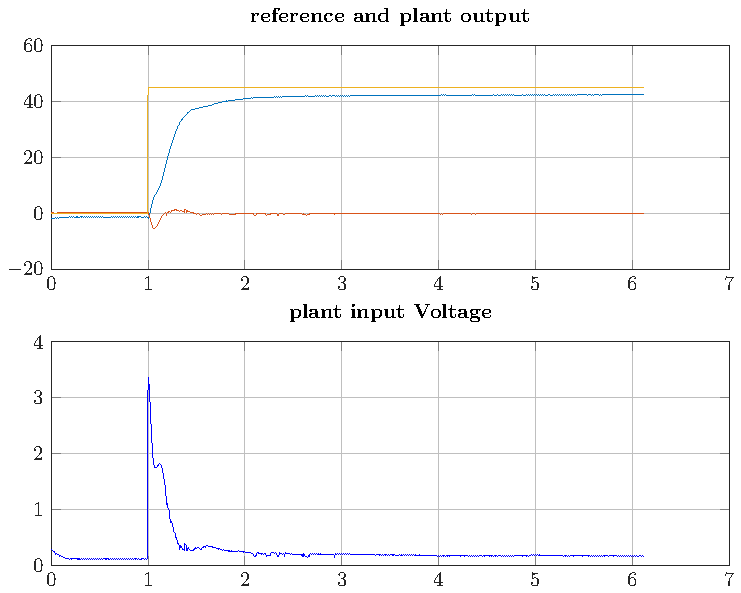
\includegraphics[scale = 0.46]{images/optimizedStepLab.pdf}
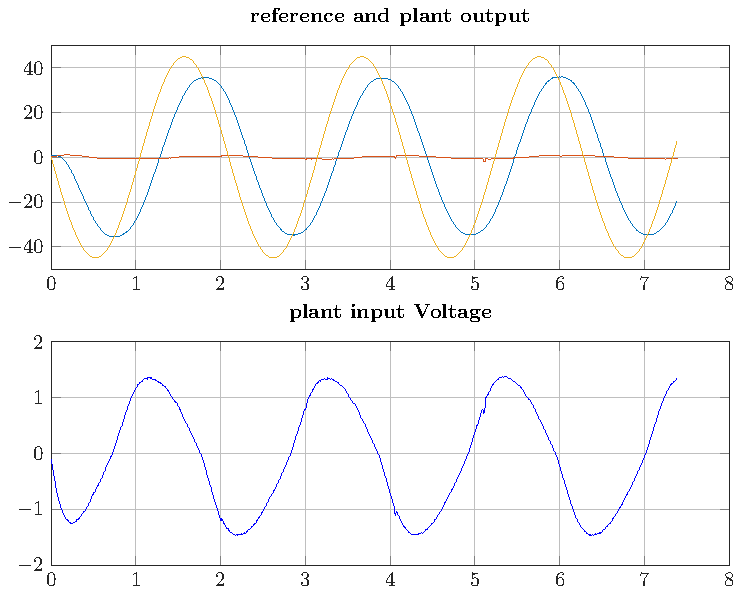
\includegraphics[scale = 0.46]{images/optimizedSineLab.pdf}
\caption{Setpoint tracking test results. References and plant outputs are given in degree [$\;^\circ$]. Plant input voltages are given in volts [V].}
\label{fig:setPoint}
\end{figure}
Using the controller we tuned during the simulation of our plant we started our experiments with some simple reference tracking experiments.\marginpar{Recall that we had the tuned controller: Q = diag([500 1000 3 10]) with R = 30.} The results are shown in figure~\ref{fig:setPoint}. In comparison to simulation~\ref{fig:allStates} results are as expected. The arm angle $\alpha$ oscillates a little less then expected. We observe a steady state offset that we did not see in our simulations, however this offset is within one or two degrees. Given that we have a small systematic error due to the potentiometer calibration that we did not fix completely this offset seems reasonable. We also applied a sinusoidal reference input. Tracking results are shown in figure\ref{fig:allStates} on the right side. In comparison to the reference sine, which has an amplitude of $45^\circ$ our system output is damped. However in the beginning we stated that apart from good tracking results we also want our controller to keep the arm angle $\alpha$ as close to zero as possible. Again we are facing a conflicting control objectives. We cannot perfectly track the hub angle $\theta$ and keep the arm angle $\alpha$ close to zero. In our experiment the arm angle $\alpha$ remained within $2$ and $-2$ degrees at all times. If we tuned more towards tracking we would loose performance here. So we are proposing this controller as a compromise. 


\end{document}
